\documentclass[twoside]{book}

% Packages required by doxygen
\usepackage{fixltx2e}
\usepackage{calc}
\usepackage{doxygen}
\usepackage{graphicx}
\usepackage[utf8]{inputenc}
\usepackage{makeidx}
\usepackage{multicol}
\usepackage{multirow}
\PassOptionsToPackage{warn}{textcomp}
\usepackage{textcomp}
\usepackage[nointegrals]{wasysym}
\usepackage[table]{xcolor}

% NLS support packages
\usepackage[french]{babel}

% Font selection
\usepackage[T1]{fontenc}
\usepackage{mathptmx}
\usepackage[scaled=.90]{helvet}
\usepackage{courier}
\usepackage{amssymb}
\usepackage{sectsty}
\renewcommand{\familydefault}{\sfdefault}
\allsectionsfont{%
  \fontseries{bc}\selectfont%
  \color{darkgray}%
}
\renewcommand{\DoxyLabelFont}{%
  \fontseries{bc}\selectfont%
  \color{darkgray}%
}
\newcommand{\+}{\discretionary{\mbox{\scriptsize$\hookleftarrow$}}{}{}}

% Page & text layout
\usepackage{geometry}
\geometry{%
  a4paper,%
  top=2.5cm,%
  bottom=2.5cm,%
  left=2.5cm,%
  right=2.5cm%
}
\tolerance=750
\hfuzz=15pt
\hbadness=750
\setlength{\emergencystretch}{15pt}
\setlength{\parindent}{0cm}
\setlength{\parskip}{0.2cm}
\makeatletter
\renewcommand{\paragraph}{%
  \@startsection{paragraph}{4}{0ex}{-1.0ex}{1.0ex}{%
    \normalfont\normalsize\bfseries\SS@parafont%
  }%
}
\renewcommand{\subparagraph}{%
  \@startsection{subparagraph}{5}{0ex}{-1.0ex}{1.0ex}{%
    \normalfont\normalsize\bfseries\SS@subparafont%
  }%
}
\makeatother

% Headers & footers
\usepackage{fancyhdr}
\pagestyle{fancyplain}
\fancyhead[LE]{\fancyplain{}{\bfseries\thepage}}
\fancyhead[CE]{\fancyplain{}{}}
\fancyhead[RE]{\fancyplain{}{\bfseries\leftmark}}
\fancyhead[LO]{\fancyplain{}{\bfseries\rightmark}}
\fancyhead[CO]{\fancyplain{}{}}
\fancyhead[RO]{\fancyplain{}{\bfseries\thepage}}
\fancyfoot[LE]{\fancyplain{}{}}
\fancyfoot[CE]{\fancyplain{}{}}
\fancyfoot[RE]{\fancyplain{}{\bfseries\scriptsize Généré le Mercredi 22 Avril 2015 21\+:36\+:00 pour Starlight par Doxygen }}
\fancyfoot[LO]{\fancyplain{}{\bfseries\scriptsize Généré le Mercredi 22 Avril 2015 21\+:36\+:00 pour Starlight par Doxygen }}
\fancyfoot[CO]{\fancyplain{}{}}
\fancyfoot[RO]{\fancyplain{}{}}
\renewcommand{\footrulewidth}{0.4pt}
\renewcommand{\chaptermark}[1]{%
  \markboth{#1}{}%
}
\renewcommand{\sectionmark}[1]{%
  \markright{\thesection\ #1}%
}

% Indices & bibliography
\usepackage{natbib}
\usepackage[titles]{tocloft}
\setcounter{tocdepth}{3}
\setcounter{secnumdepth}{5}
\makeindex

% Hyperlinks (required, but should be loaded last)
\usepackage{ifpdf}
\ifpdf
  \usepackage[pdftex,pagebackref=true]{hyperref}
\else
  \usepackage[ps2pdf,pagebackref=true]{hyperref}
\fi
\hypersetup{%
  colorlinks=true,%
  linkcolor=blue,%
  citecolor=blue,%
  unicode%
}

% Custom commands
\newcommand{\clearemptydoublepage}{%
  \newpage{\pagestyle{empty}\cleardoublepage}%
}


%===== C O N T E N T S =====

\begin{document}

% Titlepage & ToC
\hypersetup{pageanchor=false,
             bookmarks=true,
             bookmarksnumbered=true,
             pdfencoding=unicode
            }
\pagenumbering{roman}
\begin{titlepage}
\vspace*{7cm}
\begin{center}%
{\Large Starlight }\\
\vspace*{1cm}
{\large Généré par Doxygen 1.8.7}\\
\vspace*{0.5cm}
{\small Mercredi 22 Avril 2015 21:36:00}\\
\end{center}
\end{titlepage}
\clearemptydoublepage
\tableofcontents
\clearemptydoublepage
\pagenumbering{arabic}
\hypersetup{pageanchor=true}

%--- Begin generated contents ---
\chapter{Index hiérarchique}
\section{Hiérarchie des classes}
Cette liste d'héritage est classée approximativement par ordre alphabétique \+:\begin{DoxyCompactList}
\item \contentsline{section}{Element}{\pageref{d5/d3c/classElement}}{}
\begin{DoxyCompactList}
\item \contentsline{section}{Crystal}{\pageref{d6/d4f/classCrystal}}{}
\item \contentsline{section}{Dest}{\pageref{de/d97/classDest}}{}
\item \contentsline{section}{Lens}{\pageref{d6/d4b/classLens}}{}
\item \contentsline{section}{Mirror}{\pageref{de/dfd/classMirror}}{}
\item \contentsline{section}{Nuke}{\pageref{d0/ddf/classNuke}}{}
\item \contentsline{section}{Source}{\pageref{d6/d2e/classSource}}{}
\item \contentsline{section}{Wall}{\pageref{d7/dec/classWall}}{}
\end{DoxyCompactList}
\item \contentsline{section}{Ellipse}{\pageref{db/dc7/classEllipse}}{}
\item \contentsline{section}{Intersection}{\pageref{d6/d30/structIntersection}}{}
\item \contentsline{section}{Line}{\pageref{db/db6/classLine}}{}
\item \contentsline{section}{Line\+Segment}{\pageref{d1/d48/classLineSegment}}{}
\item \contentsline{section}{Map\+Reader}{\pageref{dd/d23/classMapReader}}{}
\item \contentsline{section}{Map\+Writer}{\pageref{de/d66/classMapWriter}}{}
\item \contentsline{section}{Observable}{\pageref{d9/db4/classObservable}}{}
\begin{DoxyCompactList}
\item \contentsline{section}{Crystal}{\pageref{d6/d4f/classCrystal}}{}
\item \contentsline{section}{Dest}{\pageref{de/d97/classDest}}{}
\item \contentsline{section}{Elements}{\pageref{d3/d48/classElements}}{}
\item \contentsline{section}{Lens}{\pageref{d6/d4b/classLens}}{}
\item \contentsline{section}{Level}{\pageref{d2/d9d/classLevel}}{}
\item \contentsline{section}{Map\+View}{\pageref{de/d8c/classMapView}}{}
\item \contentsline{section}{Mirror}{\pageref{de/dfd/classMirror}}{}
\item \contentsline{section}{Nuke}{\pageref{d0/ddf/classNuke}}{}
\item \contentsline{section}{Properties}{\pageref{d0/deb/classProperties}}{}
\item \contentsline{section}{Source}{\pageref{d6/d2e/classSource}}{}
\item \contentsline{section}{Wall}{\pageref{d7/dec/classWall}}{}
\end{DoxyCompactList}
\item \contentsline{section}{Observer\+Interface}{\pageref{dd/d62/classObserverInterface}}{}
\begin{DoxyCompactList}
\item \contentsline{section}{Crystal\+View}{\pageref{d3/d9b/classCrystalView}}{}
\item \contentsline{section}{Destination\+View}{\pageref{d7/d7d/classDestinationView}}{}
\item \contentsline{section}{Lens\+View}{\pageref{d6/da9/classLensView}}{}
\item \contentsline{section}{Level}{\pageref{d2/d9d/classLevel}}{}
\item \contentsline{section}{Main\+Editor}{\pageref{d3/db4/classMainEditor}}{}
\item \contentsline{section}{Map\+View}{\pageref{de/d8c/classMapView}}{}
\item \contentsline{section}{Mirror\+View}{\pageref{d6/d74/classMirrorView}}{}
\item \contentsline{section}{Nuke\+View}{\pageref{d1/dba/classNukeView}}{}
\item \contentsline{section}{Properties\+Interface}{\pageref{da/d7e/classPropertiesInterface}}{}
\begin{DoxyCompactList}
\item \contentsline{section}{Crystal\+Prop}{\pageref{d5/d35/classCrystalProp}}{}
\item \contentsline{section}{Dest\+Prop}{\pageref{dd/d85/classDestProp}}{}
\item \contentsline{section}{Lens\+Prop}{\pageref{dd/d8c/classLensProp}}{}
\item \contentsline{section}{Mirror\+Prop}{\pageref{d0/d2f/classMirrorProp}}{}
\item \contentsline{section}{Nuke\+Prop}{\pageref{df/d5e/classNukeProp}}{}
\item \contentsline{section}{Source\+Prop}{\pageref{d4/d36/classSourceProp}}{}
\item \contentsline{section}{Wall\+Prop}{\pageref{dd/dd1/classWallProp}}{}
\end{DoxyCompactList}
\item \contentsline{section}{Source\+View}{\pageref{d9/df7/classSourceView}}{}
\item \contentsline{section}{Wall\+View}{\pageref{d6/da2/classWallView}}{}
\end{DoxyCompactList}
\item \contentsline{section}{Point}{\pageref{dc/d4f/classPoint}}{}
\item Q\+Frame\begin{DoxyCompactList}
\item \contentsline{section}{Element\+View}{\pageref{d2/d81/classElementView}}{}
\begin{DoxyCompactList}
\item \contentsline{section}{Crystal\+View}{\pageref{d3/d9b/classCrystalView}}{}
\item \contentsline{section}{Destination\+View}{\pageref{d7/d7d/classDestinationView}}{}
\item \contentsline{section}{Lens\+View}{\pageref{d6/da9/classLensView}}{}
\item \contentsline{section}{Mirror\+View}{\pageref{d6/d74/classMirrorView}}{}
\item \contentsline{section}{Nuke\+View}{\pageref{d1/dba/classNukeView}}{}
\item \contentsline{section}{Source\+View}{\pageref{d9/df7/classSourceView}}{}
\item \contentsline{section}{Wall\+View}{\pageref{d6/da2/classWallView}}{}
\end{DoxyCompactList}
\end{DoxyCompactList}
\item Q\+Graphics\+Ellipse\+Item\begin{DoxyCompactList}
\item \contentsline{section}{Crystal\+View}{\pageref{d3/d9b/classCrystalView}}{}
\item \contentsline{section}{Lens\+View}{\pageref{d6/da9/classLensView}}{}
\item \contentsline{section}{Nuke\+View}{\pageref{d1/dba/classNukeView}}{}
\end{DoxyCompactList}
\item Q\+Graphics\+Line\+Item\begin{DoxyCompactList}
\item \contentsline{section}{Mirror\+View}{\pageref{d6/d74/classMirrorView}}{}
\item \contentsline{section}{Ray\+View}{\pageref{da/d1c/classRayView}}{}
\item \contentsline{section}{Wall\+View}{\pageref{d6/da2/classWallView}}{}
\end{DoxyCompactList}
\item Q\+Graphics\+Pixmap\+Item\begin{DoxyCompactList}
\item \contentsline{section}{Source\+View}{\pageref{d9/df7/classSourceView}}{}
\end{DoxyCompactList}
\item Q\+Graphics\+Rect\+Item\begin{DoxyCompactList}
\item \contentsline{section}{Button}{\pageref{d1/d19/classButton}}{}
\item \contentsline{section}{Destination\+View}{\pageref{d7/d7d/classDestinationView}}{}
\end{DoxyCompactList}
\item Q\+Graphics\+View\begin{DoxyCompactList}
\item \contentsline{section}{Main\+Menu}{\pageref{d9/d0a/classMainMenu}}{}
\item \contentsline{section}{Map\+View}{\pageref{de/d8c/classMapView}}{}
\end{DoxyCompactList}
\item Q\+Main\+Window\begin{DoxyCompactList}
\item \contentsline{section}{Main\+Editor}{\pageref{d3/db4/classMainEditor}}{}
\item \contentsline{section}{Main\+Window}{\pageref{d6/d1a/classMainWindow}}{}
\end{DoxyCompactList}
\item Q\+Object\begin{DoxyCompactList}
\item \contentsline{section}{Button}{\pageref{d1/d19/classButton}}{}
\end{DoxyCompactList}
\item Q\+Widget\begin{DoxyCompactList}
\item \contentsline{section}{Elements}{\pageref{d3/d48/classElements}}{}
\item \contentsline{section}{Properties}{\pageref{d0/deb/classProperties}}{}
\item \contentsline{section}{Properties\+Interface}{\pageref{da/d7e/classPropertiesInterface}}{}
\end{DoxyCompactList}
\item \contentsline{section}{Ray}{\pageref{d9/dce/classRay}}{}
\item \contentsline{section}{Rectangle}{\pageref{de/d00/classRectangle}}{}
\end{DoxyCompactList}

\chapter{Index des classes}
\section{Liste des classes}
Liste des classes, structures, unions et interfaces avec une brève description \+:\begin{DoxyCompactList}
\item\contentsline{section}{\hyperlink{classButton}{Button} \\*Classe représentant un bouton du menu principal }{\pageref{d1/d19/classButton}}{}
\item\contentsline{section}{\hyperlink{classCrystal}{Crystal} \\*Cette classe modélise les cristaux utilisés dans le jeu }{\pageref{d6/d4f/classCrystal}}{}
\item\contentsline{section}{\hyperlink{classCrystalProp}{Crystal\+Prop} \\*Panel permettant de modifier un cristal }{\pageref{d5/d35/classCrystalProp}}{}
\item\contentsline{section}{\hyperlink{classCrystalView}{Crystal\+View} \\*Modélisation visuelle d’un cristal }{\pageref{d3/d9b/classCrystalView}}{}
\item\contentsline{section}{\hyperlink{classDest}{Dest} \\*Cette classe modélise la destination utilisée dans le jeu }{\pageref{de/d97/classDest}}{}
\item\contentsline{section}{\hyperlink{classDestinationView}{Destination\+View} \\*Modélisation visuelle de la destination }{\pageref{d7/d7d/classDestinationView}}{}
\item\contentsline{section}{\hyperlink{classDestProp}{Dest\+Prop} \\*Panel permettant de modifier la destination }{\pageref{dd/d85/classDestProp}}{}
\item\contentsline{section}{\hyperlink{classElement}{Element} \\*Cette classe sert de super-\/classe à tous les éléments avec lesquels un rayon peut interagir }{\pageref{d5/d3c/classElement}}{}
\item\contentsline{section}{\hyperlink{classElements}{Elements} \\*Permet de créer un niveau et d’y ajouter des éléments (miroir, lensille, etc.) }{\pageref{d3/d48/classElements}}{}
\item\contentsline{section}{\hyperlink{classElementView}{Element\+View} \\*Cette classe sert de super-\/classe à tous les éléments visuels avec lesquels un rayon peut interagir }{\pageref{d2/d81/classElementView}}{}
\item\contentsline{section}{\hyperlink{classEllipse}{Ellipse} \\*Classe \hyperlink{classEllipse}{Ellipse} La position représente la position du centre de l'ellipse }{\pageref{db/dc7/classEllipse}}{}
\item\contentsline{section}{\hyperlink{structIntersection}{Intersection} \\*Structure intersection \+: Possède un élément et un point d'intersection }{\pageref{d6/d30/structIntersection}}{}
\item\contentsline{section}{\hyperlink{classLens}{Lens} \\*Cette classe modélise les lentilles utilisées dans le jeu }{\pageref{d6/d4b/classLens}}{}
\item\contentsline{section}{\hyperlink{classLensProp}{Lens\+Prop} \\*Modifie la lentille sélectionnée dans l’éditeur }{\pageref{dd/d8c/classLensProp}}{}
\item\contentsline{section}{\hyperlink{classLensView}{Lens\+View} \\*Modélisation visuelle de la lentille }{\pageref{d6/da9/classLensView}}{}
\item\contentsline{section}{\hyperlink{classLevel}{Level} \\*Modélise une carte telle qu'utilisée dans le jeu }{\pageref{d2/d9d/classLevel}}{}
\item\contentsline{section}{\hyperlink{classLine}{Line} \\*Cette classe représente une droite sous la forme ax + by + c = 0 }{\pageref{db/db6/classLine}}{}
\item\contentsline{section}{\hyperlink{classLineSegment}{Line\+Segment} \\*Modélise un segment de droite possédant un point de départ et un point d'arrivée }{\pageref{d1/d48/classLineSegment}}{}
\item\contentsline{section}{\hyperlink{classMainEditor}{Main\+Editor} \\*Fenêtre principale de l’éditeur }{\pageref{d3/db4/classMainEditor}}{}
\item\contentsline{section}{\hyperlink{classMainMenu}{Main\+Menu} \\*Représente le menu principal }{\pageref{d9/d0a/classMainMenu}}{}
\item\contentsline{section}{\hyperlink{classMainWindow}{Main\+Window} \\*Représente la fenêtre principale }{\pageref{d6/d1a/classMainWindow}}{}
\item\contentsline{section}{\hyperlink{classMapReader}{Map\+Reader} \\*Classe permettant de lire un fichier .lvl et d'instancier un niveau }{\pageref{dd/d23/classMapReader}}{}
\item\contentsline{section}{\hyperlink{classMapView}{Map\+View} \\*Modélisation visuelle d’un plateau de jeu }{\pageref{de/d8c/classMapView}}{}
\item\contentsline{section}{\hyperlink{classMapWriter}{Map\+Writer} \\*Classe permettant d'écrire un niveau dans un fichier .lvl }{\pageref{de/d66/classMapWriter}}{}
\item\contentsline{section}{\hyperlink{classMirror}{Mirror} \\*Cette classe modélise les miroirs utilisés dans le jeu }{\pageref{de/dfd/classMirror}}{}
\item\contentsline{section}{\hyperlink{classMirrorProp}{Mirror\+Prop} \\*Panel permettant de modifier un miroir }{\pageref{d0/d2f/classMirrorProp}}{}
\item\contentsline{section}{\hyperlink{classMirrorView}{Mirror\+View} \\*Modélisation visuelle d’un miroir }{\pageref{d6/d74/classMirrorView}}{}
\item\contentsline{section}{\hyperlink{classNuke}{Nuke} \\*Cette classe modélise les bombes utilisées dans le jeu }{\pageref{d0/ddf/classNuke}}{}
\item\contentsline{section}{\hyperlink{classNukeProp}{Nuke\+Prop} \\*Panel permettant de modifier une bombe }{\pageref{df/d5e/classNukeProp}}{}
\item\contentsline{section}{\hyperlink{classNukeView}{Nuke\+View} \\*Modélisation visuelle d’une bombe }{\pageref{d1/dba/classNukeView}}{}
\item\contentsline{section}{\hyperlink{classObservable}{Observable} }{\pageref{d9/db4/classObservable}}{}
\item\contentsline{section}{\hyperlink{classObserverInterface}{Observer\+Interface} }{\pageref{dd/d62/classObserverInterface}}{}
\item\contentsline{section}{\hyperlink{classPoint}{Point} \\*Cette classe modélise un simple point de coordonnées réelles utilisés pour modéliser les positions des objets dans le jeu }{\pageref{dc/d4f/classPoint}}{}
\item\contentsline{section}{\hyperlink{classProperties}{Properties} \\*Contient le widget permettant d’éditer l’élément sélectionné sur la carte et d’appliquer les changements ou de le supprimer }{\pageref{d0/deb/classProperties}}{}
\item\contentsline{section}{\hyperlink{classPropertiesInterface}{Properties\+Interface} \\*Interface représentant les propriétés d'un objet au travers d'un panel }{\pageref{da/d7e/classPropertiesInterface}}{}
\item\contentsline{section}{\hyperlink{classRay}{Ray} \\*Cette classe modélise les rayons lumineux, concept central du jeu }{\pageref{d9/dce/classRay}}{}
\item\contentsline{section}{\hyperlink{classRayView}{Ray\+View} \\*Modélisation visuelle d’un rayon de lumière }{\pageref{da/d1c/classRayView}}{}
\item\contentsline{section}{\hyperlink{classRectangle}{Rectangle} \\*Classe \hyperlink{classRectangle}{Rectangle} \+: représente un rectangle avec un point supérieur gauche, une longueur et une hauteur }{\pageref{de/d00/classRectangle}}{}
\item\contentsline{section}{\hyperlink{classSource}{Source} \\*Modélise la source lumineuse utilisée dans le jeu }{\pageref{d6/d2e/classSource}}{}
\item\contentsline{section}{\hyperlink{classSourceProp}{Source\+Prop} \\*Panel permettant de modifier la source }{\pageref{d4/d36/classSourceProp}}{}
\item\contentsline{section}{\hyperlink{classSourceView}{Source\+View} \\*Modélisation visuelle d’une source }{\pageref{d9/df7/classSourceView}}{}
\item\contentsline{section}{\hyperlink{classWall}{Wall} \\*Cette classe modélise les murs utilisés dans le jeu }{\pageref{d7/dec/classWall}}{}
\item\contentsline{section}{\hyperlink{classWallProp}{Wall\+Prop} \\*Panel permettant de modifier un mur }{\pageref{dd/dd1/classWallProp}}{}
\item\contentsline{section}{\hyperlink{classWallView}{Wall\+View} \\*Modélisation visuelle d’un mur (ne reflétant pas la lumière) }{\pageref{d6/da2/classWallView}}{}
\end{DoxyCompactList}

\chapter{Documentation des classes}
\hypertarget{classButton}{\section{Référence de la classe Button}
\label{classButton}\index{Button@{Button}}
}


Classe représentant un bouton du menu principal.  




{\ttfamily \#include $<$button.\+h$>$}



Graphe d'héritage de Button\+:\nopagebreak
\begin{figure}[H]
\begin{center}
\leavevmode
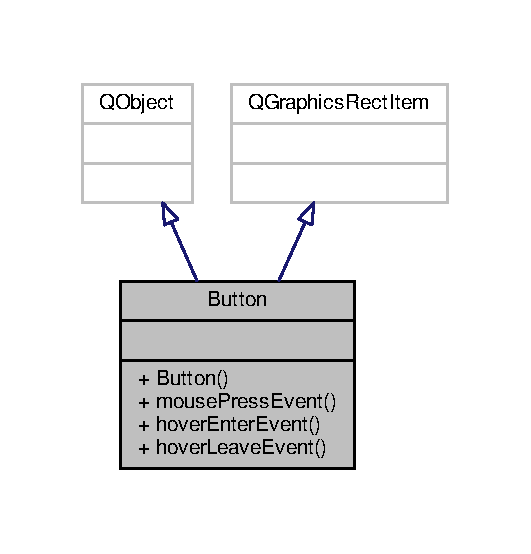
\includegraphics[width=255pt]{d5/dbb/classButton__inherit__graph}
\end{center}
\end{figure}


Graphe de collaboration de Button\+:\nopagebreak
\begin{figure}[H]
\begin{center}
\leavevmode
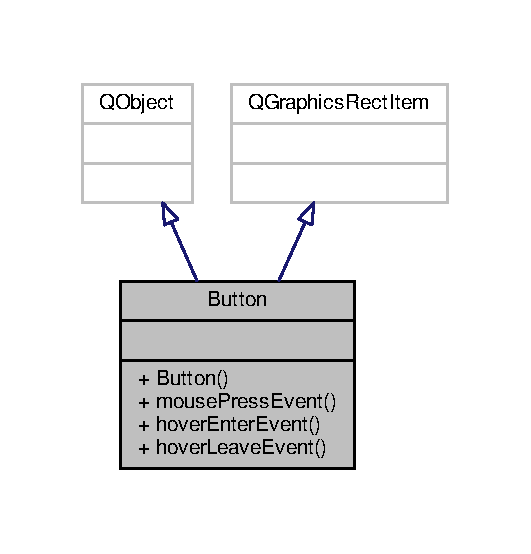
\includegraphics[width=255pt]{d6/dbf/classButton__coll__graph}
\end{center}
\end{figure}
\subsection*{Signaux}
\begin{DoxyCompactItemize}
\item 
\hypertarget{classButton_a9e7ab4152cb1e7e3beb7f2842f32670c}{void {\bfseries clicked} ()}\label{classButton_a9e7ab4152cb1e7e3beb7f2842f32670c}

\end{DoxyCompactItemize}
\subsection*{Fonctions membres publiques}
\begin{DoxyCompactItemize}
\item 
\hypertarget{classButton_a69976e5c00874a3807b642f249c1c776}{{\bfseries Button} (Q\+String name, Q\+Graphics\+Item $\ast$parent=N\+U\+L\+L)}\label{classButton_a69976e5c00874a3807b642f249c1c776}

\item 
\hypertarget{classButton_a17d8eb0c904605b223bbc00c75655315}{void {\bfseries mouse\+Press\+Event} (Q\+Graphics\+Scene\+Mouse\+Event $\ast$event)}\label{classButton_a17d8eb0c904605b223bbc00c75655315}

\item 
\hypertarget{classButton_a633a9684818bc5d300a622a00064f09c}{void {\bfseries hover\+Enter\+Event} (Q\+Graphics\+Scene\+Hover\+Event $\ast$event)}\label{classButton_a633a9684818bc5d300a622a00064f09c}

\item 
\hypertarget{classButton_a1689a97690d9469ce8350d24db0d7485}{void {\bfseries hover\+Leave\+Event} (Q\+Graphics\+Scene\+Hover\+Event $\ast$event)}\label{classButton_a1689a97690d9469ce8350d24db0d7485}

\end{DoxyCompactItemize}


\subsection{Description détaillée}
Classe représentant un bouton du menu principal. 

La documentation de cette classe a été générée à partir des fichiers suivants \+:\begin{DoxyCompactItemize}
\item 
view/button.\+h\item 
moc\+\_\+button.\+cpp\item 
view/button.\+cpp\end{DoxyCompactItemize}

\hypertarget{classCrystal}{\section{Référence de la classe Crystal}
\label{classCrystal}\index{Crystal@{Crystal}}
}


Cette classe modélise les cristaux utilisés dans le jeu.  




{\ttfamily \#include $<$crystal.\+h$>$}



Graphe d'héritage de Crystal\+:\nopagebreak
\begin{figure}[H]
\begin{center}
\leavevmode
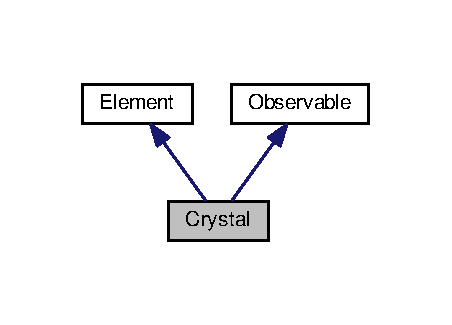
\includegraphics[width=186pt]{de/da2/classCrystal__inherit__graph}
\end{center}
\end{figure}


Graphe de collaboration de Crystal\+:\nopagebreak
\begin{figure}[H]
\begin{center}
\leavevmode
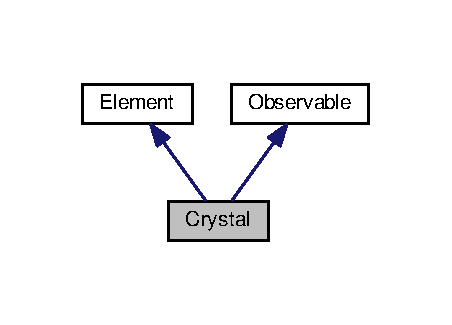
\includegraphics[width=186pt]{d4/db0/classCrystal__coll__graph}
\end{center}
\end{figure}
\subsection*{Fonctions membres publiques}
\begin{DoxyCompactItemize}
\item 
\hyperlink{classCrystal_a21597991198db73fdfe051ae1a4fec68}{Crystal} (const \hyperlink{classPoint}{Point} \&p, double r, int m)
\begin{DoxyCompactList}\small\item\em Instancie un cristal centré au point donné, d'un certain. \end{DoxyCompactList}\item 
\hyperlink{classCrystal_abcff7d0100d1f2baa0b6d993618f6a3d}{Crystal} (const \hyperlink{classCrystal}{Crystal} \&crystal)
\begin{DoxyCompactList}\small\item\em Constructeur de copie. \end{DoxyCompactList}\item 
const \hyperlink{classPoint}{Point} \& \hyperlink{classCrystal_a6c817c9e47ec46b632a02c8098373562}{center} () const 
\begin{DoxyCompactList}\small\item\em Retourne la coordonnée du centre du cristal. \end{DoxyCompactList}\item 
int \hyperlink{classCrystal_a227a44060d81139b167f1f8ed2b2e2a9}{modifier} () const 
\begin{DoxyCompactList}\small\item\em Retourne le modificateur de longueur d'onde du cristal. \end{DoxyCompactList}\item 
double \hyperlink{classCrystal_abad9d6b77ef64effbd692a445fb0fead}{radius} () const 
\begin{DoxyCompactList}\small\item\em Retourne le rayon du cristal. \end{DoxyCompactList}\item 
void \hyperlink{classCrystal_a3639d10c52b98d93bc81f21fb6e2e929}{set\+\_\+center} (const \hyperlink{classPoint}{Point} \&c)
\begin{DoxyCompactList}\small\item\em Modifie la coordonée du centre du cristal. \end{DoxyCompactList}\item 
void \hyperlink{classCrystal_a05a53bb4f4d519248d62990f8a62b786}{set\+\_\+radius} (const double rad)
\begin{DoxyCompactList}\small\item\em Modifie le rayon du cristal. \end{DoxyCompactList}\item 
void \hyperlink{classCrystal_a9aaadd11a8fc70932b998073f67df8fe}{set\+\_\+modifier} (const double mod)
\begin{DoxyCompactList}\small\item\em Modifie le modificateur de longueur d’onde du cristal. \end{DoxyCompactList}\item 
void \hyperlink{classCrystal_a1369f8ba73c1fbbc4df22cda83d9fe7c}{translate} (const double x, const double y)
\begin{DoxyCompactList}\small\item\em Déplace le cristal. \end{DoxyCompactList}\item 
\hyperlink{classEllipse}{Ellipse} \hyperlink{classCrystal_a57617a62778965048bcea6b22e9d6f48}{to\+\_\+ellipse} () const 
\begin{DoxyCompactList}\small\item\em Retourne l'ellipse correspondante au cristal. \end{DoxyCompactList}\item 
bool \hyperlink{classCrystal_a882bf87d3b3c0dd2c4fbecbbb9d1c066}{operator==} (const \hyperlink{classCrystal}{Crystal} \&c) const 
\begin{DoxyCompactList}\small\item\em Redéfinition de l'opérateur d'égalité, retourne vrai si les cristaux sont égaux. \end{DoxyCompactList}\end{DoxyCompactItemize}
\subsection*{Amis}
\begin{DoxyCompactItemize}
\item 
std\+::ostream \& \hyperlink{classCrystal_a45da91e3993e90a57a5f4fd5edda0adb}{operator$<$$<$} (std\+::ostream \&, const \hyperlink{classCrystal}{Crystal} \&)
\begin{DoxyCompactList}\small\item\em Surcharge l'opérateur de flux de sortie pour afficher. \end{DoxyCompactList}\end{DoxyCompactItemize}
\subsection*{Membres hérités additionnels}


\subsection{Description détaillée}
Cette classe modélise les cristaux utilisés dans le jeu. 

Un cristal est un objet circulaire centré en un point, et d'un certain rayon. 

Un rayon lumineux passant à travers un cristal modifie sa longueur d'onde (en l'augmentant ou en la diminuant d'une certaine valeur) mais pas sa trajectoire. 

\subsection{Documentation des constructeurs et destructeur}
\hypertarget{classCrystal_a21597991198db73fdfe051ae1a4fec68}{\index{Crystal@{Crystal}!Crystal@{Crystal}}
\index{Crystal@{Crystal}!Crystal@{Crystal}}
\subsubsection[{Crystal}]{\setlength{\rightskip}{0pt plus 5cm}Crystal\+::\+Crystal (
\begin{DoxyParamCaption}
\item[{const {\bf Point} \&}]{p, }
\item[{double}]{r, }
\item[{int}]{m}
\end{DoxyParamCaption}
)}}\label{classCrystal_a21597991198db73fdfe051ae1a4fec68}


Instancie un cristal centré au point donné, d'un certain. 

rayon et modifiant la longueur d'onde des rayons qui le traversent d'une valeur donnée. 
\begin{DoxyParams}{Paramètres}
{\em p} & le centre du cristal. \\
\hline
{\em r} & le rayon du cristal. \\
\hline
{\em m} & le modificateur de longueur d'onde du cristal. \\
\hline
\end{DoxyParams}
\hypertarget{classCrystal_abcff7d0100d1f2baa0b6d993618f6a3d}{\index{Crystal@{Crystal}!Crystal@{Crystal}}
\index{Crystal@{Crystal}!Crystal@{Crystal}}
\subsubsection[{Crystal}]{\setlength{\rightskip}{0pt plus 5cm}Crystal\+::\+Crystal (
\begin{DoxyParamCaption}
\item[{const {\bf Crystal} \&}]{crystal}
\end{DoxyParamCaption}
)}}\label{classCrystal_abcff7d0100d1f2baa0b6d993618f6a3d}


Constructeur de copie. 


\begin{DoxyParams}{Paramètres}
{\em crystal} & le cristal à copier. \\
\hline
\end{DoxyParams}


\subsection{Documentation des fonctions membres}
\hypertarget{classCrystal_a6c817c9e47ec46b632a02c8098373562}{\index{Crystal@{Crystal}!center@{center}}
\index{center@{center}!Crystal@{Crystal}}
\subsubsection[{center}]{\setlength{\rightskip}{0pt plus 5cm}const {\bf Point} \& Crystal\+::center (
\begin{DoxyParamCaption}
{}
\end{DoxyParamCaption}
) const\hspace{0.3cm}{\ttfamily [inline]}}}\label{classCrystal_a6c817c9e47ec46b632a02c8098373562}


Retourne la coordonnée du centre du cristal. 

\begin{DoxyReturn}{Renvoie}
la coordonnée du centre du cristal. 
\end{DoxyReturn}
\hypertarget{classCrystal_a227a44060d81139b167f1f8ed2b2e2a9}{\index{Crystal@{Crystal}!modifier@{modifier}}
\index{modifier@{modifier}!Crystal@{Crystal}}
\subsubsection[{modifier}]{\setlength{\rightskip}{0pt plus 5cm}int Crystal\+::modifier (
\begin{DoxyParamCaption}
{}
\end{DoxyParamCaption}
) const\hspace{0.3cm}{\ttfamily [inline]}}}\label{classCrystal_a227a44060d81139b167f1f8ed2b2e2a9}


Retourne le modificateur de longueur d'onde du cristal. 

\begin{DoxyReturn}{Renvoie}
le modificateur de longueur d'onde du cristal. 
\end{DoxyReturn}
\hypertarget{classCrystal_a882bf87d3b3c0dd2c4fbecbbb9d1c066}{\index{Crystal@{Crystal}!operator==@{operator==}}
\index{operator==@{operator==}!Crystal@{Crystal}}
\subsubsection[{operator==}]{\setlength{\rightskip}{0pt plus 5cm}bool Crystal\+::operator== (
\begin{DoxyParamCaption}
\item[{const {\bf Crystal} \&}]{c}
\end{DoxyParamCaption}
) const}}\label{classCrystal_a882bf87d3b3c0dd2c4fbecbbb9d1c066}


Redéfinition de l'opérateur d'égalité, retourne vrai si les cristaux sont égaux. 


\begin{DoxyParams}{Paramètres}
{\em c} & un cristal. \\
\hline
\end{DoxyParams}
\begin{DoxyReturn}{Renvoie}
vrai si les cristaux sont égaux, faux sinon. 
\end{DoxyReturn}
\hypertarget{classCrystal_abad9d6b77ef64effbd692a445fb0fead}{\index{Crystal@{Crystal}!radius@{radius}}
\index{radius@{radius}!Crystal@{Crystal}}
\subsubsection[{radius}]{\setlength{\rightskip}{0pt plus 5cm}double Crystal\+::radius (
\begin{DoxyParamCaption}
{}
\end{DoxyParamCaption}
) const\hspace{0.3cm}{\ttfamily [inline]}}}\label{classCrystal_abad9d6b77ef64effbd692a445fb0fead}


Retourne le rayon du cristal. 

\begin{DoxyReturn}{Renvoie}
le rayon du cristal. 
\end{DoxyReturn}
\hypertarget{classCrystal_a3639d10c52b98d93bc81f21fb6e2e929}{\index{Crystal@{Crystal}!set\+\_\+center@{set\+\_\+center}}
\index{set\+\_\+center@{set\+\_\+center}!Crystal@{Crystal}}
\subsubsection[{set\+\_\+center}]{\setlength{\rightskip}{0pt plus 5cm}void Crystal\+::set\+\_\+center (
\begin{DoxyParamCaption}
\item[{const {\bf Point} \&}]{c}
\end{DoxyParamCaption}
)\hspace{0.3cm}{\ttfamily [inline]}}}\label{classCrystal_a3639d10c52b98d93bc81f21fb6e2e929}


Modifie la coordonée du centre du cristal. 


\begin{DoxyParams}{Paramètres}
{\em c} & le nouveau centre du cristal. \\
\hline
\end{DoxyParams}
\hypertarget{classCrystal_a9aaadd11a8fc70932b998073f67df8fe}{\index{Crystal@{Crystal}!set\+\_\+modifier@{set\+\_\+modifier}}
\index{set\+\_\+modifier@{set\+\_\+modifier}!Crystal@{Crystal}}
\subsubsection[{set\+\_\+modifier}]{\setlength{\rightskip}{0pt plus 5cm}void Crystal\+::set\+\_\+modifier (
\begin{DoxyParamCaption}
\item[{const double}]{mod}
\end{DoxyParamCaption}
)\hspace{0.3cm}{\ttfamily [inline]}}}\label{classCrystal_a9aaadd11a8fc70932b998073f67df8fe}


Modifie le modificateur de longueur d’onde du cristal. 


\begin{DoxyParams}{Paramètres}
{\em mod} & le modificateur de longueur d’onde du cristal. \\
\hline
\end{DoxyParams}
\hypertarget{classCrystal_a05a53bb4f4d519248d62990f8a62b786}{\index{Crystal@{Crystal}!set\+\_\+radius@{set\+\_\+radius}}
\index{set\+\_\+radius@{set\+\_\+radius}!Crystal@{Crystal}}
\subsubsection[{set\+\_\+radius}]{\setlength{\rightskip}{0pt plus 5cm}void Crystal\+::set\+\_\+radius (
\begin{DoxyParamCaption}
\item[{const double}]{rad}
\end{DoxyParamCaption}
)\hspace{0.3cm}{\ttfamily [inline]}}}\label{classCrystal_a05a53bb4f4d519248d62990f8a62b786}


Modifie le rayon du cristal. 


\begin{DoxyParams}{Paramètres}
{\em rad} & le nouveau rayon du cristal. \\
\hline
\end{DoxyParams}
\hypertarget{classCrystal_a57617a62778965048bcea6b22e9d6f48}{\index{Crystal@{Crystal}!to\+\_\+ellipse@{to\+\_\+ellipse}}
\index{to\+\_\+ellipse@{to\+\_\+ellipse}!Crystal@{Crystal}}
\subsubsection[{to\+\_\+ellipse}]{\setlength{\rightskip}{0pt plus 5cm}{\bf Ellipse} Crystal\+::to\+\_\+ellipse (
\begin{DoxyParamCaption}
{}
\end{DoxyParamCaption}
) const}}\label{classCrystal_a57617a62778965048bcea6b22e9d6f48}


Retourne l'ellipse correspondante au cristal. 

\begin{DoxyReturn}{Renvoie}
l'ellipse correspondante au cristal. 
\end{DoxyReturn}
\hypertarget{classCrystal_a1369f8ba73c1fbbc4df22cda83d9fe7c}{\index{Crystal@{Crystal}!translate@{translate}}
\index{translate@{translate}!Crystal@{Crystal}}
\subsubsection[{translate}]{\setlength{\rightskip}{0pt plus 5cm}void Crystal\+::translate (
\begin{DoxyParamCaption}
\item[{const double}]{x, }
\item[{const double}]{y}
\end{DoxyParamCaption}
)}}\label{classCrystal_a1369f8ba73c1fbbc4df22cda83d9fe7c}


Déplace le cristal. 


\begin{DoxyParams}{Paramètres}
{\em x} & le déplacement sur l'axe x. \\
\hline
{\em y} & le déplacement sur l'axe y. \\
\hline
\end{DoxyParams}


\subsection{Documentation des fonctions amies et associées}
\hypertarget{classCrystal_a45da91e3993e90a57a5f4fd5edda0adb}{\index{Crystal@{Crystal}!operator$<$$<$@{operator$<$$<$}}
\index{operator$<$$<$@{operator$<$$<$}!Crystal@{Crystal}}
\subsubsection[{operator$<$$<$}]{\setlength{\rightskip}{0pt plus 5cm}std\+::ostream\& operator$<$$<$ (
\begin{DoxyParamCaption}
\item[{std\+::ostream \&}]{out, }
\item[{const {\bf Crystal} \&}]{c}
\end{DoxyParamCaption}
)\hspace{0.3cm}{\ttfamily [friend]}}}\label{classCrystal_a45da91e3993e90a57a5f4fd5edda0adb}


Surcharge l'opérateur de flux de sortie pour afficher. 

un récapitulatif des caractéristiques du cristal sous-\/jacent en console. \begin{DoxyReturn}{Renvoie}
le flux dans lequel le cristal a été imprimé. 
\end{DoxyReturn}


La documentation de cette classe a été générée à partir des fichiers suivants \+:\begin{DoxyCompactItemize}
\item 
model/crystal.\+h\item 
model/crystal.\+cpp\end{DoxyCompactItemize}

\hypertarget{classCrystalProp}{\section{Référence de la classe Crystal\+Prop}
\label{classCrystalProp}\index{Crystal\+Prop@{Crystal\+Prop}}
}


Panel permettant de modifier un cristal.  




{\ttfamily \#include $<$crystalprop.\+h$>$}



Graphe d'héritage de Crystal\+Prop\+:
\nopagebreak
\begin{figure}[H]
\begin{center}
\leavevmode
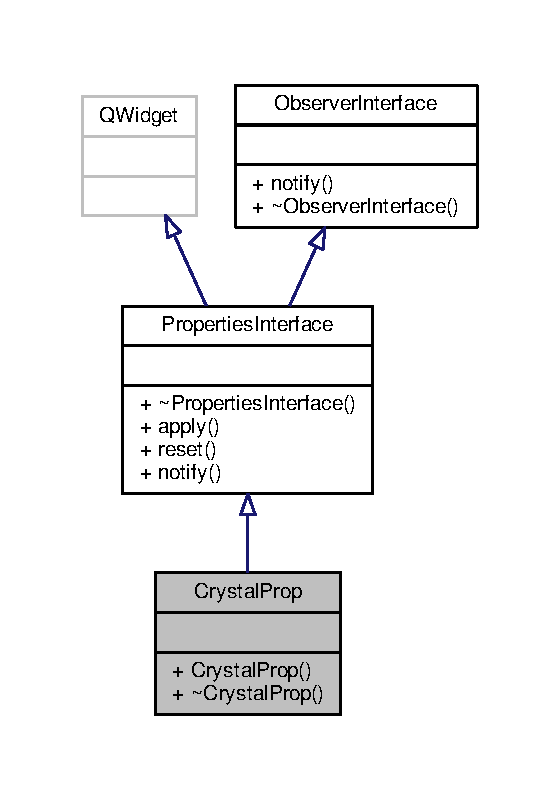
\includegraphics[width=269pt]{d8/d57/classCrystalProp__inherit__graph}
\end{center}
\end{figure}


Graphe de collaboration de Crystal\+Prop\+:
\nopagebreak
\begin{figure}[H]
\begin{center}
\leavevmode
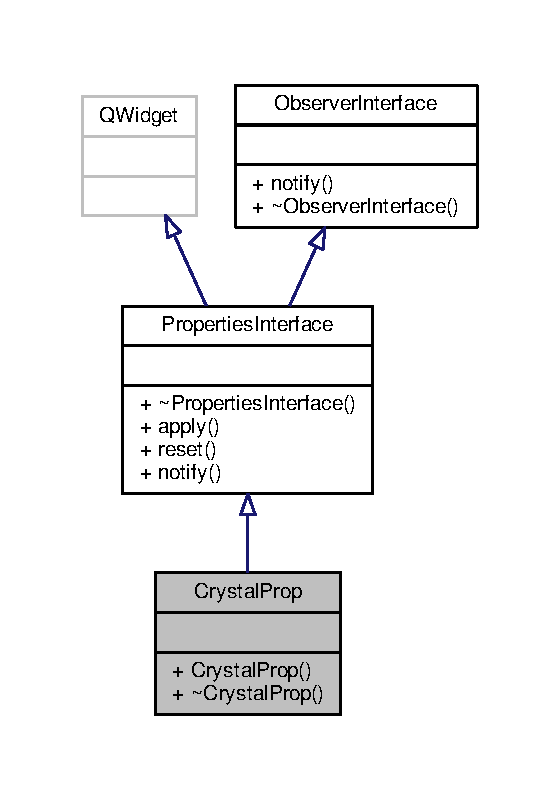
\includegraphics[width=269pt]{d0/d15/classCrystalProp__coll__graph}
\end{center}
\end{figure}
\subsection*{Fonctions membres publiques}
\begin{DoxyCompactItemize}
\item 
\hyperlink{classCrystalProp_a47068eadccacdada66efdec58235ce94}{Crystal\+Prop} (\hyperlink{classCrystal}{Crystal} $\ast$crystal, Q\+Widget $\ast$parent=0)
\begin{DoxyCompactList}\small\item\em Instancie un panel de propriétés pour un cristal. \end{DoxyCompactList}\end{DoxyCompactItemize}


\subsection{Description détaillée}
Panel permettant de modifier un cristal. 

\subsection{Documentation des constructeurs et destructeur}
\hypertarget{classCrystalProp_a47068eadccacdada66efdec58235ce94}{\index{Crystal\+Prop@{Crystal\+Prop}!Crystal\+Prop@{Crystal\+Prop}}
\index{Crystal\+Prop@{Crystal\+Prop}!Crystal\+Prop@{Crystal\+Prop}}
\subsubsection[{Crystal\+Prop}]{\setlength{\rightskip}{0pt plus 5cm}Crystal\+Prop\+::\+Crystal\+Prop (
\begin{DoxyParamCaption}
\item[{{\bf Crystal} $\ast$}]{crystal, }
\item[{Q\+Widget $\ast$}]{parent = {\ttfamily 0}}
\end{DoxyParamCaption}
)}}\label{classCrystalProp_a47068eadccacdada66efdec58235ce94}


Instancie un panel de propriétés pour un cristal. 

Modifie le cristal sélectionné dans l’éditeur.


\begin{DoxyParams}{Paramètres}
{\em crystal} & le cristal. \\
\hline
{\em parent} & le parent.\\
\hline
{\em crystal} & le cristal sélectionné. \\
\hline
{\em parent} & le widget parent. \\
\hline
\end{DoxyParams}


La documentation de cette classe a été générée à partir des fichiers suivants \+:\begin{DoxyCompactItemize}
\item 
editor/crystalprop.\+h\item 
editor/crystalprop.\+cpp\end{DoxyCompactItemize}

\hypertarget{classCrystalView}{\section{Référence de la classe Crystal\+View}
\label{classCrystalView}\index{Crystal\+View@{Crystal\+View}}
}


Modélisation visuelle d’un cristal.  




{\ttfamily \#include $<$crystalview.\+h$>$}



Graphe d'héritage de Crystal\+View\+:\nopagebreak
\begin{figure}[H]
\begin{center}
\leavevmode
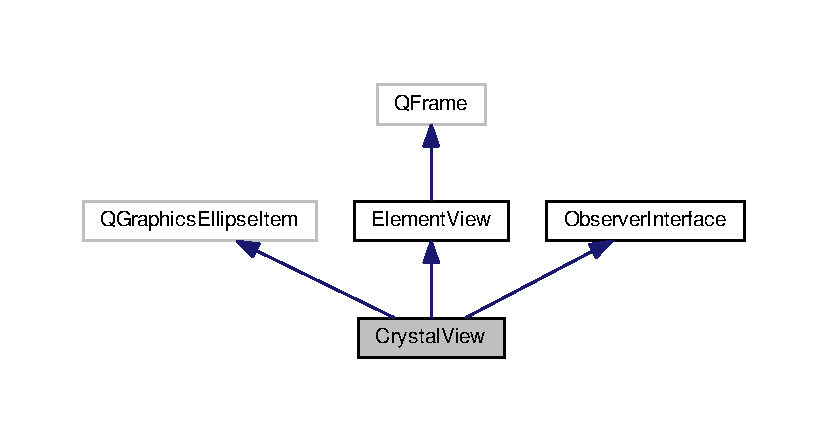
\includegraphics[width=350pt]{d8/d3c/classCrystalView__inherit__graph}
\end{center}
\end{figure}


Graphe de collaboration de Crystal\+View\+:\nopagebreak
\begin{figure}[H]
\begin{center}
\leavevmode
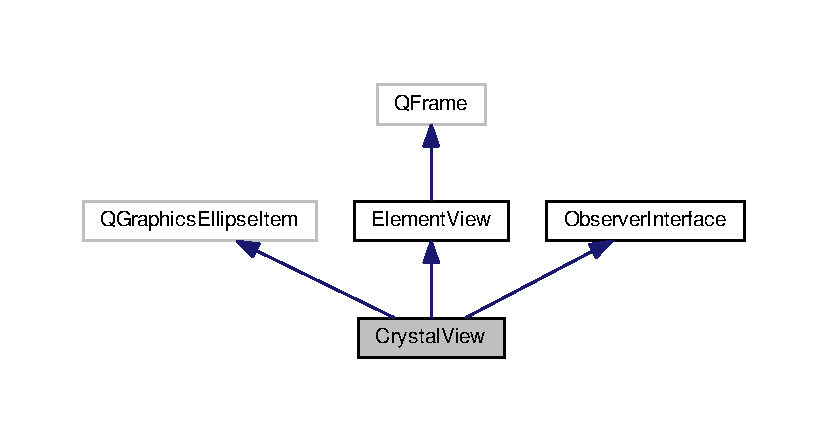
\includegraphics[width=350pt]{d0/d09/classCrystalView__coll__graph}
\end{center}
\end{figure}
\subsection*{Fonctions membres publiques}
\begin{DoxyCompactItemize}
\item 
\hypertarget{classCrystalView_a82ec82a190920476f9ae64aca5691ceb}{{\bfseries Crystal\+View} (const \hyperlink{classCrystal}{Crystal} \&crystal, bool selectable=false)}\label{classCrystalView_a82ec82a190920476f9ae64aca5691ceb}

\item 
\hypertarget{classCrystalView_a0168a3da89580fb0c5467f88c635ac9f}{\hyperlink{classCrystal}{Crystal} $\ast$ {\bfseries crystal} ()}\label{classCrystalView_a0168a3da89580fb0c5467f88c635ac9f}

\item 
\hypertarget{classCrystalView_a6fffe79b15c269a44f9c393ed163f205}{bool {\bfseries selectable} () const }\label{classCrystalView_a6fffe79b15c269a44f9c393ed163f205}

\item 
\hypertarget{classCrystalView_ab2a8ffda8203f9d645fa137ba8542ce4}{void {\bfseries set\+\_\+selectable} (bool value)}\label{classCrystalView_ab2a8ffda8203f9d645fa137ba8542ce4}

\item 
\hypertarget{classCrystalView_adc16471475cf13a0cd815f587ae0b012}{void {\bfseries translate} (double x=.\+0, double y=.\+0)}\label{classCrystalView_adc16471475cf13a0cd815f587ae0b012}

\item 
void \hyperlink{classCrystalView_a167f2bc5e7fd6e7daaca9fc39e475806}{notify} (\hyperlink{classObservable}{Observable} $\ast$sdo, std\+::string msg, const std\+::vector$<$ std\+::string $>$ \&args=std\+::vector$<$ std\+::string $>$())
\begin{DoxyCompactList}\small\item\em Notifie le jeu d'un évènement provenant d'un sujet d'observation (\hyperlink{classObservable}{Observable}). \end{DoxyCompactList}\end{DoxyCompactItemize}
\subsection*{Membres hérités additionnels}


\subsection{Description détaillée}
Modélisation visuelle d’un cristal. 

\subsection{Documentation des fonctions membres}
\hypertarget{classCrystalView_a167f2bc5e7fd6e7daaca9fc39e475806}{\index{Crystal\+View@{Crystal\+View}!notify@{notify}}
\index{notify@{notify}!Crystal\+View@{Crystal\+View}}
\subsubsection[{notify}]{\setlength{\rightskip}{0pt plus 5cm}void Crystal\+View\+::notify (
\begin{DoxyParamCaption}
\item[{{\bf Observable} $\ast$}]{sdo, }
\item[{std\+::string}]{msg, }
\item[{const std\+::vector$<$ std\+::string $>$ \&}]{args = {\ttfamily std\+:\+:vector$<$~std\+:\+:string~$>$()}}
\end{DoxyParamCaption}
)\hspace{0.3cm}{\ttfamily [virtual]}}}\label{classCrystalView_a167f2bc5e7fd6e7daaca9fc39e475806}


Notifie le jeu d'un évènement provenant d'un sujet d'observation (\hyperlink{classObservable}{Observable}). 


\begin{DoxyParams}{Paramètres}
{\em o} & l'observé. \\
\hline
{\em msg} & le message de notification. \\
\hline
{\em args} & des arguments. \\
\hline
\end{DoxyParams}


Implémente \hyperlink{classObserverInterface_a1bbd22519c2942d978804714db12c8b2}{Observer\+Interface}.



La documentation de cette classe a été générée à partir des fichiers suivants \+:\begin{DoxyCompactItemize}
\item 
view/crystalview.\+h\item 
view/crystalview.\+cpp\end{DoxyCompactItemize}

\hypertarget{classDest}{\section{Référence de la classe Dest}
\label{classDest}\index{Dest@{Dest}}
}


Cette classe modélise la destination utilisée dans le jeu.  




{\ttfamily \#include $<$dest.\+h$>$}



Graphe d'héritage de Dest\+:
\nopagebreak
\begin{figure}[H]
\begin{center}
\leavevmode
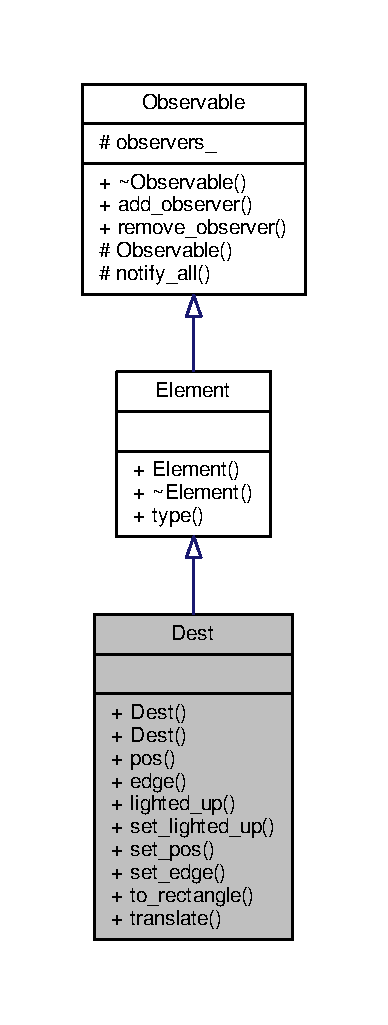
\includegraphics[width=186pt]{d9/d5c/classDest__inherit__graph}
\end{center}
\end{figure}


Graphe de collaboration de Dest\+:
\nopagebreak
\begin{figure}[H]
\begin{center}
\leavevmode
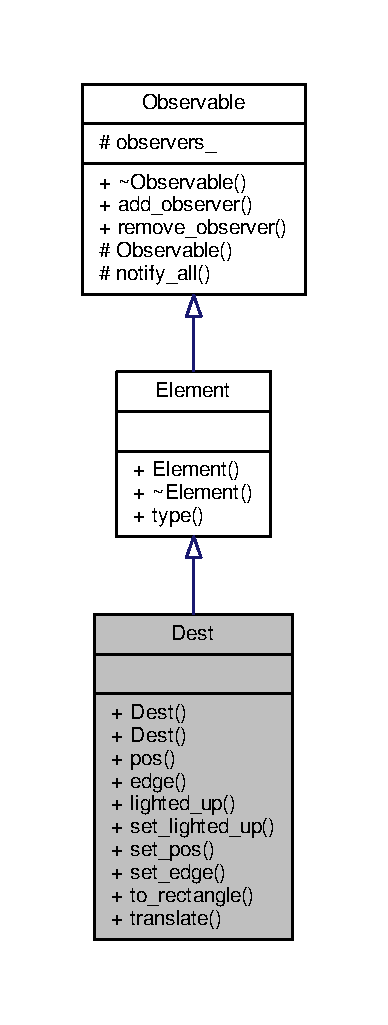
\includegraphics[width=186pt]{d4/d77/classDest__coll__graph}
\end{center}
\end{figure}
\subsection*{Fonctions membres publiques}
\begin{DoxyCompactItemize}
\item 
\hyperlink{classDest_ac4b55b2569af4d98a6b265becf8922a7}{Dest} (const \hyperlink{classPoint}{Point} \&p, double e)
\begin{DoxyCompactList}\small\item\em Intancie une destination de position et rayon donné. \end{DoxyCompactList}\item 
\hyperlink{classDest_ad5bc62f6c24692e9ca8116c0b43d8dbb}{Dest} (const \hyperlink{classDest}{Dest} \&dest)
\begin{DoxyCompactList}\small\item\em Constructeur de copie. \end{DoxyCompactList}\item 
const \hyperlink{classPoint}{Point} \& \hyperlink{classDest_a40eed96fe590c1ecc354239dfed73b5e}{pos} () const 
\begin{DoxyCompactList}\small\item\em Retourne la position du coin supérieur gauche du carré. \end{DoxyCompactList}\item 
double \hyperlink{classDest_a3a8acfcc4637300fe240c299881c5c61}{edge} () const 
\begin{DoxyCompactList}\small\item\em Retourne la longueur du côté du carré représentant la destination. \end{DoxyCompactList}\item 
bool \hyperlink{classDest_af549b51a5ddf4cbdab7e95e0e07ee5d4}{lighted\+\_\+up} () const 
\begin{DoxyCompactList}\small\item\em Retourne vrai si la destination est illuminée, faux sinon. \end{DoxyCompactList}\item 
void \hyperlink{classDest_a52ab303c379e3f541692effccf183329}{set\+\_\+lighted\+\_\+up} (const bool value)
\begin{DoxyCompactList}\small\item\em Illumine la destination ou non. \end{DoxyCompactList}\item 
void \hyperlink{classDest_acdf685e262d90814429717f3270e215f}{set\+\_\+pos} (const \hyperlink{classPoint}{Point} \&\hyperlink{classDest_a40eed96fe590c1ecc354239dfed73b5e}{pos})
\begin{DoxyCompactList}\small\item\em Modifie la position du coin supérieur gauche du carré. \end{DoxyCompactList}\item 
void \hyperlink{classDest_af6c4c76da5373925c8b605faabb187f9}{set\+\_\+edge} (const double \hyperlink{classDest_a3a8acfcc4637300fe240c299881c5c61}{edge})
\begin{DoxyCompactList}\small\item\em Modifie la longueur du côté du carré représentant la destination. \end{DoxyCompactList}\item 
\hyperlink{classRectangle}{Rectangle} \hyperlink{classDest_a5af0475a453bf4ae292907b0f65ecd76}{to\+\_\+rectangle} ()
\begin{DoxyCompactList}\small\item\em Retourne le rectangle correspondant à la destination. \end{DoxyCompactList}\item 
void \hyperlink{classDest_a5a45df42c8960e3bcf510338acc04c99}{translate} (const double x, const double y)
\begin{DoxyCompactList}\small\item\em Déplace la destination. \end{DoxyCompactList}\end{DoxyCompactItemize}
\subsection*{Amis}
\begin{DoxyCompactItemize}
\item 
std\+::ostream \& \hyperlink{classDest_a256a3d2bff5f10395424d5dc911a2b4e}{operator$<$$<$} (std\+::ostream \&out, const \hyperlink{classDest}{Dest} \&s)
\begin{DoxyCompactList}\small\item\em Surcharge l'opérateur de flux de sortie pour afficher. \end{DoxyCompactList}\end{DoxyCompactItemize}
\subsection*{Membres hérités additionnels}


\subsection{Description détaillée}
Cette classe modélise la destination utilisée dans le jeu. 

Une destination est un objet carré qui, quand traversé par un rayon lumineux, fait remporter la partie au joueur. 

\subsection{Documentation des constructeurs et destructeur}
\hypertarget{classDest_ac4b55b2569af4d98a6b265becf8922a7}{\index{Dest@{Dest}!Dest@{Dest}}
\index{Dest@{Dest}!Dest@{Dest}}
\subsubsection[{Dest}]{\setlength{\rightskip}{0pt plus 5cm}Dest\+::\+Dest (
\begin{DoxyParamCaption}
\item[{const {\bf Point} \&}]{p, }
\item[{double}]{e}
\end{DoxyParamCaption}
)}}\label{classDest_ac4b55b2569af4d98a6b265becf8922a7}


Intancie une destination de position et rayon donné. 


\begin{DoxyParams}{Paramètres}
{\em p} & le coin supérieur gauche du carré modélisant la destination. \\
\hline
{\em e} & la longueur du côté du carré. \\
\hline
\end{DoxyParams}
\hypertarget{classDest_ad5bc62f6c24692e9ca8116c0b43d8dbb}{\index{Dest@{Dest}!Dest@{Dest}}
\index{Dest@{Dest}!Dest@{Dest}}
\subsubsection[{Dest}]{\setlength{\rightskip}{0pt plus 5cm}Dest\+::\+Dest (
\begin{DoxyParamCaption}
\item[{const {\bf Dest} \&}]{dest}
\end{DoxyParamCaption}
)}}\label{classDest_ad5bc62f6c24692e9ca8116c0b43d8dbb}


Constructeur de copie. 


\begin{DoxyParams}{Paramètres}
{\em dest} & la destination à copier. \\
\hline
\end{DoxyParams}


\subsection{Documentation des fonctions membres}
\hypertarget{classDest_a3a8acfcc4637300fe240c299881c5c61}{\index{Dest@{Dest}!edge@{edge}}
\index{edge@{edge}!Dest@{Dest}}
\subsubsection[{edge}]{\setlength{\rightskip}{0pt plus 5cm}double Dest\+::edge (
\begin{DoxyParamCaption}
{}
\end{DoxyParamCaption}
) const\hspace{0.3cm}{\ttfamily [inline]}}}\label{classDest_a3a8acfcc4637300fe240c299881c5c61}


Retourne la longueur du côté du carré représentant la destination. 

\begin{DoxyReturn}{Renvoie}
la longueur du côté du carré représentant la destination. 
\end{DoxyReturn}
\hypertarget{classDest_af549b51a5ddf4cbdab7e95e0e07ee5d4}{\index{Dest@{Dest}!lighted\+\_\+up@{lighted\+\_\+up}}
\index{lighted\+\_\+up@{lighted\+\_\+up}!Dest@{Dest}}
\subsubsection[{lighted\+\_\+up}]{\setlength{\rightskip}{0pt plus 5cm}bool Dest\+::lighted\+\_\+up (
\begin{DoxyParamCaption}
{}
\end{DoxyParamCaption}
) const\hspace{0.3cm}{\ttfamily [inline]}}}\label{classDest_af549b51a5ddf4cbdab7e95e0e07ee5d4}


Retourne vrai si la destination est illuminée, faux sinon. 

\begin{DoxyReturn}{Renvoie}
vrai si la destination est illuminée, faux sinon. 
\end{DoxyReturn}
\hypertarget{classDest_a40eed96fe590c1ecc354239dfed73b5e}{\index{Dest@{Dest}!pos@{pos}}
\index{pos@{pos}!Dest@{Dest}}
\subsubsection[{pos}]{\setlength{\rightskip}{0pt plus 5cm}const {\bf Point} \& Dest\+::pos (
\begin{DoxyParamCaption}
{}
\end{DoxyParamCaption}
) const\hspace{0.3cm}{\ttfamily [inline]}}}\label{classDest_a40eed96fe590c1ecc354239dfed73b5e}


Retourne la position du coin supérieur gauche du carré. 

modélisant la destination. \begin{DoxyReturn}{Renvoie}
la position de la destination. 
\end{DoxyReturn}
\hypertarget{classDest_af6c4c76da5373925c8b605faabb187f9}{\index{Dest@{Dest}!set\+\_\+edge@{set\+\_\+edge}}
\index{set\+\_\+edge@{set\+\_\+edge}!Dest@{Dest}}
\subsubsection[{set\+\_\+edge}]{\setlength{\rightskip}{0pt plus 5cm}void Dest\+::set\+\_\+edge (
\begin{DoxyParamCaption}
\item[{const double}]{edge}
\end{DoxyParamCaption}
)\hspace{0.3cm}{\ttfamily [inline]}}}\label{classDest_af6c4c76da5373925c8b605faabb187f9}


Modifie la longueur du côté du carré représentant la destination. 


\begin{DoxyParams}{Paramètres}
{\em edge} & la nouvelle longueur du côté de la destination. \\
\hline
\end{DoxyParams}
\hypertarget{classDest_a52ab303c379e3f541692effccf183329}{\index{Dest@{Dest}!set\+\_\+lighted\+\_\+up@{set\+\_\+lighted\+\_\+up}}
\index{set\+\_\+lighted\+\_\+up@{set\+\_\+lighted\+\_\+up}!Dest@{Dest}}
\subsubsection[{set\+\_\+lighted\+\_\+up}]{\setlength{\rightskip}{0pt plus 5cm}void Dest\+::set\+\_\+lighted\+\_\+up (
\begin{DoxyParamCaption}
\item[{const bool}]{value}
\end{DoxyParamCaption}
)\hspace{0.3cm}{\ttfamily [inline]}}}\label{classDest_a52ab303c379e3f541692effccf183329}


Illumine la destination ou non. 


\begin{DoxyParams}{Paramètres}
{\em value} & vrai si la destination doit être illuminée, faux sinon. \\
\hline
\end{DoxyParams}
\hypertarget{classDest_acdf685e262d90814429717f3270e215f}{\index{Dest@{Dest}!set\+\_\+pos@{set\+\_\+pos}}
\index{set\+\_\+pos@{set\+\_\+pos}!Dest@{Dest}}
\subsubsection[{set\+\_\+pos}]{\setlength{\rightskip}{0pt plus 5cm}void Dest\+::set\+\_\+pos (
\begin{DoxyParamCaption}
\item[{const {\bf Point} \&}]{pos}
\end{DoxyParamCaption}
)\hspace{0.3cm}{\ttfamily [inline]}}}\label{classDest_acdf685e262d90814429717f3270e215f}


Modifie la position du coin supérieur gauche du carré. 


\begin{DoxyParams}{Paramètres}
{\em pos} & la nouvelle position du coin supérieur gauche de la destination. \\
\hline
\end{DoxyParams}
\hypertarget{classDest_a5af0475a453bf4ae292907b0f65ecd76}{\index{Dest@{Dest}!to\+\_\+rectangle@{to\+\_\+rectangle}}
\index{to\+\_\+rectangle@{to\+\_\+rectangle}!Dest@{Dest}}
\subsubsection[{to\+\_\+rectangle}]{\setlength{\rightskip}{0pt plus 5cm}{\bf Rectangle} Dest\+::to\+\_\+rectangle (
\begin{DoxyParamCaption}
{}
\end{DoxyParamCaption}
)}}\label{classDest_a5af0475a453bf4ae292907b0f65ecd76}


Retourne le rectangle correspondant à la destination. 

\begin{DoxyReturn}{Renvoie}
le rectangle correspondant à la destination. 
\end{DoxyReturn}
\hypertarget{classDest_a5a45df42c8960e3bcf510338acc04c99}{\index{Dest@{Dest}!translate@{translate}}
\index{translate@{translate}!Dest@{Dest}}
\subsubsection[{translate}]{\setlength{\rightskip}{0pt plus 5cm}void Dest\+::translate (
\begin{DoxyParamCaption}
\item[{const double}]{x, }
\item[{const double}]{y}
\end{DoxyParamCaption}
)}}\label{classDest_a5a45df42c8960e3bcf510338acc04c99}


Déplace la destination. 


\begin{DoxyParams}{Paramètres}
{\em x} & le déplacement sur l'axe x. \\
\hline
{\em y} & le déplacement sur l'axe y. \\
\hline
\end{DoxyParams}


\subsection{Documentation des fonctions amies et associées}
\hypertarget{classDest_a256a3d2bff5f10395424d5dc911a2b4e}{\index{Dest@{Dest}!operator$<$$<$@{operator$<$$<$}}
\index{operator$<$$<$@{operator$<$$<$}!Dest@{Dest}}
\subsubsection[{operator$<$$<$}]{\setlength{\rightskip}{0pt plus 5cm}std\+::ostream\& operator$<$$<$ (
\begin{DoxyParamCaption}
\item[{std\+::ostream \&}]{out, }
\item[{const {\bf Dest} \&}]{s}
\end{DoxyParamCaption}
)\hspace{0.3cm}{\ttfamily [friend]}}}\label{classDest_a256a3d2bff5f10395424d5dc911a2b4e}


Surcharge l'opérateur de flux de sortie pour afficher. 

un récapitulatif des caractéristiques de la destination sous-\/jacente en console. \begin{DoxyReturn}{Renvoie}
le flux dans lequel la destination a été imprimée. 
\end{DoxyReturn}


La documentation de cette classe a été générée à partir des fichiers suivants \+:\begin{DoxyCompactItemize}
\item 
model/dest.\+h\item 
model/dest.\+cpp\end{DoxyCompactItemize}

\hypertarget{classDestinationView}{\section{Référence de la classe Destination\+View}
\label{classDestinationView}\index{Destination\+View@{Destination\+View}}
}


Modélisation visuelle de la destination.  




{\ttfamily \#include $<$destinationview.\+h$>$}



Graphe d'héritage de Destination\+View\+:
\nopagebreak
\begin{figure}[H]
\begin{center}
\leavevmode
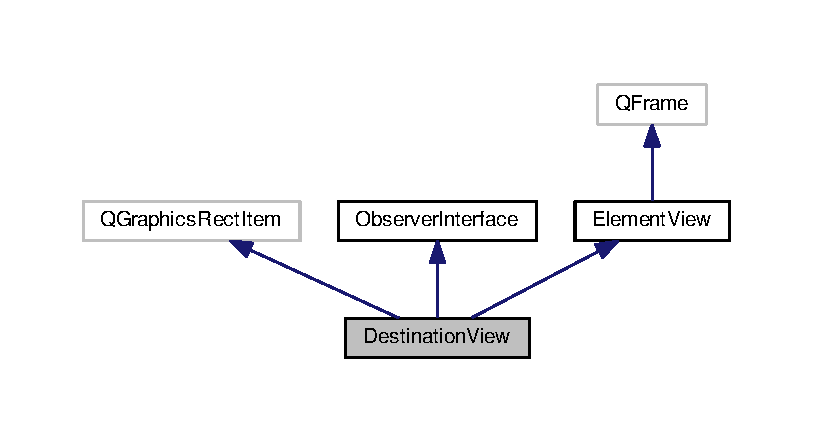
\includegraphics[width=350pt]{d6/d79/classDestinationView__inherit__graph}
\end{center}
\end{figure}


Graphe de collaboration de Destination\+View\+:
\nopagebreak
\begin{figure}[H]
\begin{center}
\leavevmode
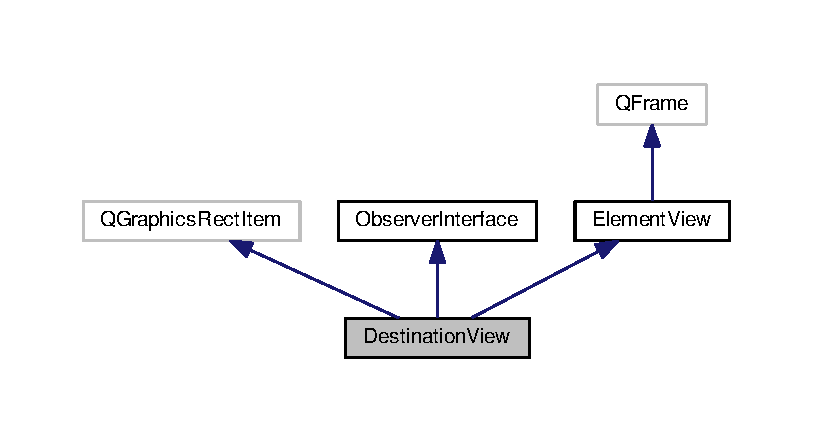
\includegraphics[width=350pt]{d0/d46/classDestinationView__coll__graph}
\end{center}
\end{figure}
\subsection*{Fonctions membres publiques}
\begin{DoxyCompactItemize}
\item 
\hyperlink{classDestinationView_ade423541028697f01a4892830471881d}{Destination\+View} (const \hyperlink{classDest}{Dest} \&dest, bool selectable=false)
\begin{DoxyCompactList}\small\item\em Construit une destination carrée. \end{DoxyCompactList}\item 
\hypertarget{classDestinationView_ae8afc4d5eceb09a0d8ff478b20f1fa1d}{\hyperlink{classDest}{Dest} $\ast$ {\bfseries dest} ()}\label{classDestinationView_ae8afc4d5eceb09a0d8ff478b20f1fa1d}

\item 
\hypertarget{classDestinationView_a2193a64a9d58d0faa80fa5c0541af638}{bool {\bfseries selectable} () const }\label{classDestinationView_a2193a64a9d58d0faa80fa5c0541af638}

\item 
\hypertarget{classDestinationView_a8e3dd1c269161b43a4b903092550ba5d}{void {\bfseries set\+\_\+selectable} (bool value)}\label{classDestinationView_a8e3dd1c269161b43a4b903092550ba5d}

\item 
\hypertarget{classDestinationView_aa3efb1f232a1e459b270ce047bc94796}{void {\bfseries translate} (double x=.\+0, double y=.\+0)}\label{classDestinationView_aa3efb1f232a1e459b270ce047bc94796}

\item 
void \hyperlink{classDestinationView_a2db4a98a3103b3b8aeaf6ae5a56847a7}{notify} (\hyperlink{classObservable}{Observable} $\ast$sdo, std\+::string msg, const std\+::vector$<$ std\+::string $>$ \&args=std\+::vector$<$ std\+::string $>$())
\begin{DoxyCompactList}\small\item\em Notifie le jeu d'un évènement provenant d'un sujet d'observation (\hyperlink{classObservable}{Observable}). \end{DoxyCompactList}\end{DoxyCompactItemize}
\subsection*{Membres hérités additionnels}


\subsection{Description détaillée}
Modélisation visuelle de la destination. 

\subsection{Documentation des constructeurs et destructeur}
\hypertarget{classDestinationView_ade423541028697f01a4892830471881d}{\index{Destination\+View@{Destination\+View}!Destination\+View@{Destination\+View}}
\index{Destination\+View@{Destination\+View}!Destination\+View@{Destination\+View}}
\subsubsection[{Destination\+View}]{\setlength{\rightskip}{0pt plus 5cm}Destination\+View\+::\+Destination\+View (
\begin{DoxyParamCaption}
\item[{const {\bf Dest} \&}]{dest, }
\item[{bool}]{selectable = {\ttfamily false}}
\end{DoxyParamCaption}
)}}\label{classDestinationView_ade423541028697f01a4892830471881d}


Construit une destination carrée. 


\begin{DoxyParams}{Paramètres}
{\em pos\+X} & abscisse du point supérieur gauche. \\
\hline
{\em pos\+Y} & ordonnée du point supérieur gauche. \\
\hline
{\em width} & longueur de la destination. \\
\hline
{\em height} & hauteur de la destination. \\
\hline
\end{DoxyParams}


\subsection{Documentation des fonctions membres}
\hypertarget{classDestinationView_a2db4a98a3103b3b8aeaf6ae5a56847a7}{\index{Destination\+View@{Destination\+View}!notify@{notify}}
\index{notify@{notify}!Destination\+View@{Destination\+View}}
\subsubsection[{notify}]{\setlength{\rightskip}{0pt plus 5cm}void Destination\+View\+::notify (
\begin{DoxyParamCaption}
\item[{{\bf Observable} $\ast$}]{sdo, }
\item[{std\+::string}]{msg, }
\item[{const std\+::vector$<$ std\+::string $>$ \&}]{args = {\ttfamily std\+:\+:vector$<$~std\+:\+:string~$>$()}}
\end{DoxyParamCaption}
)\hspace{0.3cm}{\ttfamily [virtual]}}}\label{classDestinationView_a2db4a98a3103b3b8aeaf6ae5a56847a7}


Notifie le jeu d'un évènement provenant d'un sujet d'observation (\hyperlink{classObservable}{Observable}). 


\begin{DoxyParams}{Paramètres}
{\em o} & l'observé. \\
\hline
{\em msg} & le message de notification. \\
\hline
{\em args} & des arguments. \\
\hline
\end{DoxyParams}


Implémente \hyperlink{classObserverInterface_a1bbd22519c2942d978804714db12c8b2}{Observer\+Interface}.



La documentation de cette classe a été générée à partir des fichiers suivants \+:\begin{DoxyCompactItemize}
\item 
view/destinationview.\+h\item 
view/destinationview.\+cpp\end{DoxyCompactItemize}

\hypertarget{classDestProp}{\section{Référence de la classe Dest\+Prop}
\label{classDestProp}\index{Dest\+Prop@{Dest\+Prop}}
}


Panel permettant de modifier la destination.  




{\ttfamily \#include $<$destprop.\+h$>$}



Graphe d'héritage de Dest\+Prop\+:\nopagebreak
\begin{figure}[H]
\begin{center}
\leavevmode
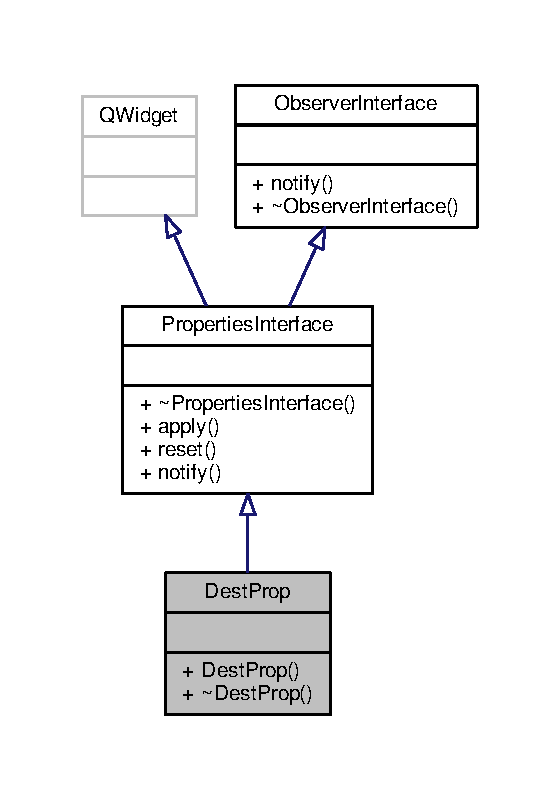
\includegraphics[width=269pt]{d4/d2d/classDestProp__inherit__graph}
\end{center}
\end{figure}


Graphe de collaboration de Dest\+Prop\+:\nopagebreak
\begin{figure}[H]
\begin{center}
\leavevmode
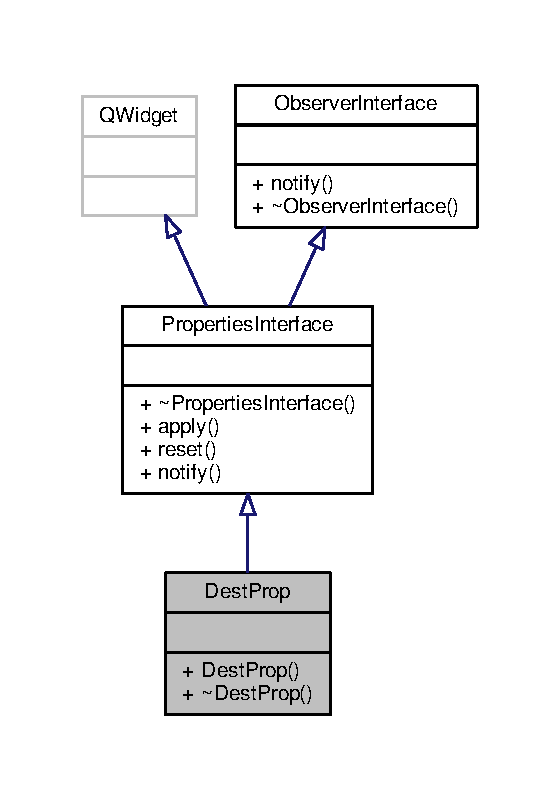
\includegraphics[width=269pt]{d4/d2b/classDestProp__coll__graph}
\end{center}
\end{figure}
\subsection*{Fonctions membres publiques}
\begin{DoxyCompactItemize}
\item 
\hypertarget{classDestProp_accf41a3f4a376030696fca6daff74cff}{{\bfseries Dest\+Prop} (\hyperlink{classDest}{Dest} $\ast$dest, Q\+Widget $\ast$parent=0)}\label{classDestProp_accf41a3f4a376030696fca6daff74cff}

\end{DoxyCompactItemize}


\subsection{Description détaillée}
Panel permettant de modifier la destination. 

La documentation de cette classe a été générée à partir des fichiers suivants \+:\begin{DoxyCompactItemize}
\item 
editor/destprop.\+h\item 
editor/destprop.\+cpp\end{DoxyCompactItemize}

\hypertarget{classElement}{\section{Référence de la classe Element}
\label{classElement}\index{Element@{Element}}
}


Cette classe sert de super-\/classe à tous les éléments avec lesquels un rayon peut interagir.  




{\ttfamily \#include $<$element.\+h$>$}



Graphe d'héritage de Element\+:\nopagebreak
\begin{figure}[H]
\begin{center}
\leavevmode
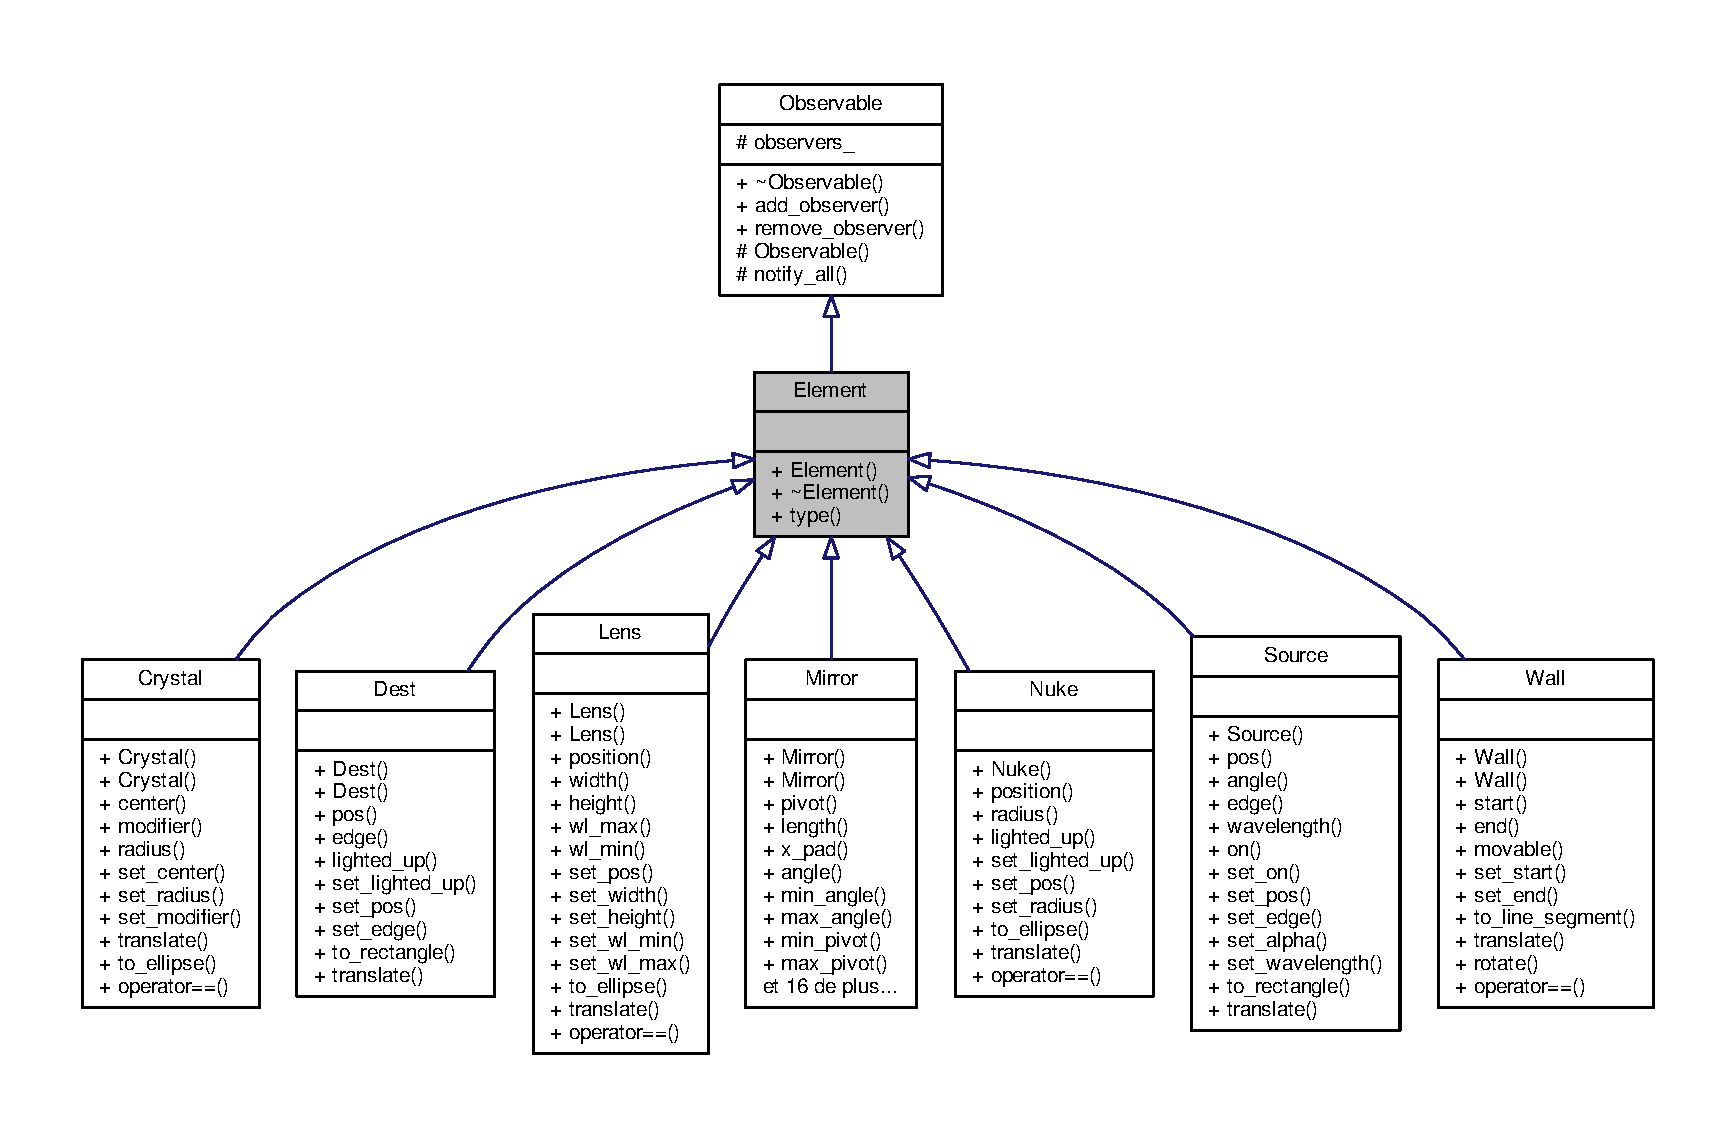
\includegraphics[width=350pt]{d8/dd6/classElement__inherit__graph}
\end{center}
\end{figure}


Graphe de collaboration de Element\+:\nopagebreak
\begin{figure}[H]
\begin{center}
\leavevmode
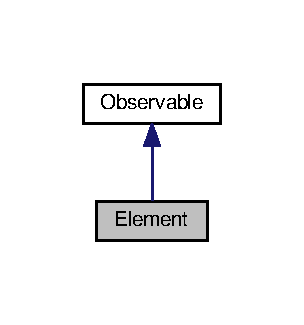
\includegraphics[width=146pt]{d4/dd1/classElement__coll__graph}
\end{center}
\end{figure}
\subsection*{Types publics}
\begin{DoxyCompactItemize}
\item 
\hypertarget{classElement_a009a3be4c3a037a72e292b2464c9cbc5}{enum {\bfseries Type} \{ \\*
{\bfseries M\+I\+R\+R\+O\+R}, 
{\bfseries C\+R\+Y\+S\+T\+A\+L}, 
{\bfseries L\+E\+N\+S}, 
{\bfseries D\+E\+S\+T}, 
\\*
{\bfseries S\+O\+U\+R\+C\+E}, 
{\bfseries N\+U\+K\+E}, 
{\bfseries W\+A\+L\+L}
 \}}\label{classElement_a009a3be4c3a037a72e292b2464c9cbc5}

\end{DoxyCompactItemize}
\subsection*{Fonctions membres publiques}
\begin{DoxyCompactItemize}
\item 
\hypertarget{classElement_a0715913621e7695aba3b04d4d5fd140d}{\hyperlink{classElement_a0715913621e7695aba3b04d4d5fd140d}{Element} (Element\+::\+Type \hyperlink{classElement_a4c4d133a897618ffc6fe397b18593bc2}{type})}\label{classElement_a0715913621e7695aba3b04d4d5fd140d}

\begin{DoxyCompactList}\small\item\em Construit un élément avec un type permettant de connaître le type de l'élément à tout moment. \end{DoxyCompactList}\item 
const Type \& \hyperlink{classElement_a4c4d133a897618ffc6fe397b18593bc2}{type} () const 
\begin{DoxyCompactList}\small\item\em Retourne le type de l'élément. \end{DoxyCompactList}\end{DoxyCompactItemize}
\subsection*{Attributs publics}
\begin{DoxyCompactItemize}
\item 
\hypertarget{classElement_a3a623be6c6790403d4e585c587b813e2}{Type {\bfseries type\+\_\+}}\label{classElement_a3a623be6c6790403d4e585c587b813e2}

\end{DoxyCompactItemize}
\subsection*{Membres hérités additionnels}


\subsection{Description détaillée}
Cette classe sert de super-\/classe à tous les éléments avec lesquels un rayon peut interagir. 

Il s'agit plus d'une classe \char`\"{}\+T\+A\+G\char`\"{} pour retrouver le type d'un élément. 

\subsection{Documentation des fonctions membres}
\hypertarget{classElement_a4c4d133a897618ffc6fe397b18593bc2}{\index{Element@{Element}!type@{type}}
\index{type@{type}!Element@{Element}}
\subsubsection[{type}]{\setlength{\rightskip}{0pt plus 5cm}const Element\+::\+Type \& Element\+::type (
\begin{DoxyParamCaption}
{}
\end{DoxyParamCaption}
) const\hspace{0.3cm}{\ttfamily [inline]}}}\label{classElement_a4c4d133a897618ffc6fe397b18593bc2}


Retourne le type de l'élément. 

\begin{DoxyReturn}{Renvoie}
le type de l'élément. 
\end{DoxyReturn}


La documentation de cette classe a été générée à partir du fichier suivant \+:\begin{DoxyCompactItemize}
\item 
model/element.\+h\end{DoxyCompactItemize}

\hypertarget{classElements}{\section{Référence de la classe Elements}
\label{classElements}\index{Elements@{Elements}}
}


Permet de créer un niveau et d’y ajouter des éléments (miroir, lensille, etc.).  




{\ttfamily \#include $<$elements.\+h$>$}



Graphe d'héritage de Elements\+:\nopagebreak
\begin{figure}[H]
\begin{center}
\leavevmode
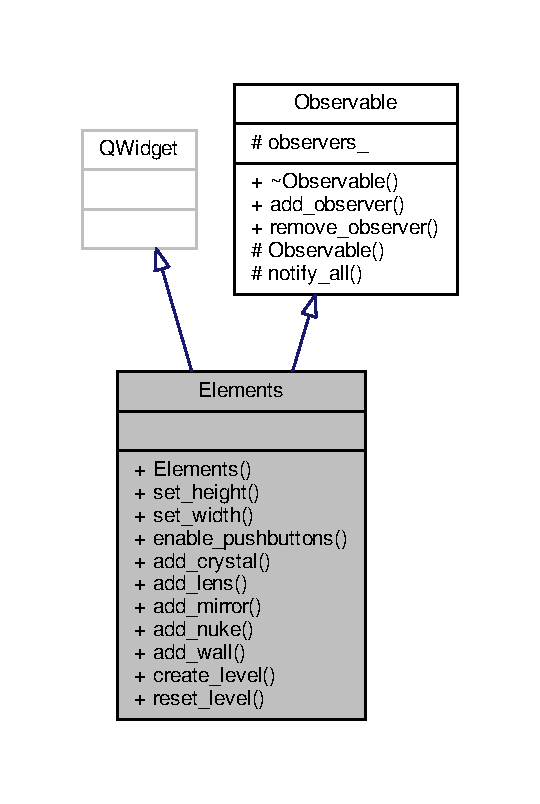
\includegraphics[width=259pt]{da/d2c/classElements__inherit__graph}
\end{center}
\end{figure}


Graphe de collaboration de Elements\+:\nopagebreak
\begin{figure}[H]
\begin{center}
\leavevmode
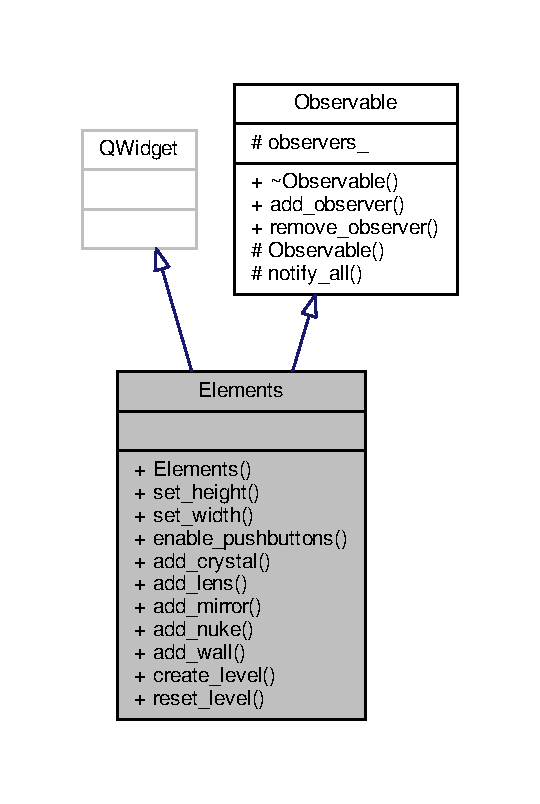
\includegraphics[width=259pt]{d3/d60/classElements__coll__graph}
\end{center}
\end{figure}
\subsection*{Connecteurs publics}
\begin{DoxyCompactItemize}
\item 
void \hyperlink{classElements_a964576c05a5b9ec733a663474f8fd978}{add\+\_\+crystal} ()
\begin{DoxyCompactList}\small\item\em Ajoute un cristal au niveau. \end{DoxyCompactList}\item 
void \hyperlink{classElements_a8093eca3330566813da371aecc96530c}{add\+\_\+lens} ()
\begin{DoxyCompactList}\small\item\em Ajoute une lentille au niveau. \end{DoxyCompactList}\item 
void \hyperlink{classElements_a8d7a4e7ff0c84f105f0f0116425293a7}{add\+\_\+mirror} ()
\begin{DoxyCompactList}\small\item\em Ajoute un miroir au niveau. \end{DoxyCompactList}\item 
void \hyperlink{classElements_aa0884faf781bb26d6ca4dd8751b0eb32}{add\+\_\+nuke} ()
\begin{DoxyCompactList}\small\item\em Ajoute une bombe au niveau. \end{DoxyCompactList}\item 
void \hyperlink{classElements_ad4b05e8a07d9f6867035243c5e3f7572}{add\+\_\+wall} ()
\begin{DoxyCompactList}\small\item\em Ajoute un mur au niveau. \end{DoxyCompactList}\item 
\hypertarget{classElements_ad4bfaa4ea43fffd8653224165b5bbc29}{void \hyperlink{classElements_ad4bfaa4ea43fffd8653224165b5bbc29}{create\+\_\+level} ()}\label{classElements_ad4bfaa4ea43fffd8653224165b5bbc29}

\begin{DoxyCompactList}\small\item\em Crée un nouveau niveau avec les dimensions précisées. \end{DoxyCompactList}\item 
\hypertarget{classElements_a938cdaf6c97d1c9e5db80280b6379176}{void \hyperlink{classElements_a938cdaf6c97d1c9e5db80280b6379176}{reset\+\_\+level} ()}\label{classElements_a938cdaf6c97d1c9e5db80280b6379176}

\begin{DoxyCompactList}\small\item\em Supprime le niveau actuel. \end{DoxyCompactList}\end{DoxyCompactItemize}
\subsection*{Fonctions membres publiques}
\begin{DoxyCompactItemize}
\item 
\hypertarget{classElements_a2b73500c747cc879fe708d35aba45532}{{\bfseries Elements} (Q\+Widget $\ast$parent=0)}\label{classElements_a2b73500c747cc879fe708d35aba45532}

\item 
\hyperlink{classLevel}{Level} $\ast$ \hyperlink{classElements_add91eac75df596342176acac4eb8b1a1}{level} ()
\begin{DoxyCompactList}\small\item\em Retourne le niveau. \end{DoxyCompactList}\item 
void \hyperlink{classElements_a077b89b923b450bda172001121825e03}{set\+\_\+height} (int h)
\begin{DoxyCompactList}\small\item\em Modifie la taille du niveau. \end{DoxyCompactList}\item 
void \hyperlink{classElements_af6c7af0c40d3840296224453352fc534}{set\+\_\+width} (int w)
\begin{DoxyCompactList}\small\item\em Modifie la largeur du niveau. \end{DoxyCompactList}\item 
\hypertarget{classElements_ac8411c290c41dcb1777cb649155d3c04}{void {\bfseries enable\+\_\+pushbuttons} (bool b)}\label{classElements_ac8411c290c41dcb1777cb649155d3c04}

\end{DoxyCompactItemize}
\subsection*{Membres hérités additionnels}


\subsection{Description détaillée}
Permet de créer un niveau et d’y ajouter des éléments (miroir, lensille, etc.). 

\subsection{Documentation des fonctions membres}
\hypertarget{classElements_a964576c05a5b9ec733a663474f8fd978}{\index{Elements@{Elements}!add\+\_\+crystal@{add\+\_\+crystal}}
\index{add\+\_\+crystal@{add\+\_\+crystal}!Elements@{Elements}}
\subsubsection[{add\+\_\+crystal}]{\setlength{\rightskip}{0pt plus 5cm}void Elements\+::add\+\_\+crystal (
\begin{DoxyParamCaption}
{}
\end{DoxyParamCaption}
)\hspace{0.3cm}{\ttfamily [slot]}}}\label{classElements_a964576c05a5b9ec733a663474f8fd978}


Ajoute un cristal au niveau. 

Indique à tous les observateurs qu’un cristal a été ajouté. \hypertarget{classElements_a8093eca3330566813da371aecc96530c}{\index{Elements@{Elements}!add\+\_\+lens@{add\+\_\+lens}}
\index{add\+\_\+lens@{add\+\_\+lens}!Elements@{Elements}}
\subsubsection[{add\+\_\+lens}]{\setlength{\rightskip}{0pt plus 5cm}void Elements\+::add\+\_\+lens (
\begin{DoxyParamCaption}
{}
\end{DoxyParamCaption}
)\hspace{0.3cm}{\ttfamily [slot]}}}\label{classElements_a8093eca3330566813da371aecc96530c}


Ajoute une lentille au niveau. 

Indique à tous les observateurs qu’une lentille a été ajoutée. \hypertarget{classElements_a8d7a4e7ff0c84f105f0f0116425293a7}{\index{Elements@{Elements}!add\+\_\+mirror@{add\+\_\+mirror}}
\index{add\+\_\+mirror@{add\+\_\+mirror}!Elements@{Elements}}
\subsubsection[{add\+\_\+mirror}]{\setlength{\rightskip}{0pt plus 5cm}void Elements\+::add\+\_\+mirror (
\begin{DoxyParamCaption}
{}
\end{DoxyParamCaption}
)\hspace{0.3cm}{\ttfamily [slot]}}}\label{classElements_a8d7a4e7ff0c84f105f0f0116425293a7}


Ajoute un miroir au niveau. 

Indique à tous les observateurs qu’un miroir a été ajouté. \hypertarget{classElements_aa0884faf781bb26d6ca4dd8751b0eb32}{\index{Elements@{Elements}!add\+\_\+nuke@{add\+\_\+nuke}}
\index{add\+\_\+nuke@{add\+\_\+nuke}!Elements@{Elements}}
\subsubsection[{add\+\_\+nuke}]{\setlength{\rightskip}{0pt plus 5cm}void Elements\+::add\+\_\+nuke (
\begin{DoxyParamCaption}
{}
\end{DoxyParamCaption}
)\hspace{0.3cm}{\ttfamily [slot]}}}\label{classElements_aa0884faf781bb26d6ca4dd8751b0eb32}


Ajoute une bombe au niveau. 

Indique à tous les observateurs qu’une bombe a été ajoutée. \hypertarget{classElements_ad4b05e8a07d9f6867035243c5e3f7572}{\index{Elements@{Elements}!add\+\_\+wall@{add\+\_\+wall}}
\index{add\+\_\+wall@{add\+\_\+wall}!Elements@{Elements}}
\subsubsection[{add\+\_\+wall}]{\setlength{\rightskip}{0pt plus 5cm}void Elements\+::add\+\_\+wall (
\begin{DoxyParamCaption}
{}
\end{DoxyParamCaption}
)\hspace{0.3cm}{\ttfamily [slot]}}}\label{classElements_ad4b05e8a07d9f6867035243c5e3f7572}


Ajoute un mur au niveau. 

Indique à tous les observateurs qu’un mur a été ajouté. \hypertarget{classElements_add91eac75df596342176acac4eb8b1a1}{\index{Elements@{Elements}!level@{level}}
\index{level@{level}!Elements@{Elements}}
\subsubsection[{level}]{\setlength{\rightskip}{0pt plus 5cm}{\bf Level} $\ast$ Elements\+::level (
\begin{DoxyParamCaption}
{}
\end{DoxyParamCaption}
)}}\label{classElements_add91eac75df596342176acac4eb8b1a1}


Retourne le niveau. 

\begin{DoxyReturn}{Renvoie}
le niveau. 
\end{DoxyReturn}
\hypertarget{classElements_a077b89b923b450bda172001121825e03}{\index{Elements@{Elements}!set\+\_\+height@{set\+\_\+height}}
\index{set\+\_\+height@{set\+\_\+height}!Elements@{Elements}}
\subsubsection[{set\+\_\+height}]{\setlength{\rightskip}{0pt plus 5cm}void Elements\+::set\+\_\+height (
\begin{DoxyParamCaption}
\item[{int}]{h}
\end{DoxyParamCaption}
)}}\label{classElements_a077b89b923b450bda172001121825e03}


Modifie la taille du niveau. 


\begin{DoxyParams}{Paramètres}
{\em h} & la hauteur de la carte du niveau. \\
\hline
\end{DoxyParams}
\hypertarget{classElements_af6c7af0c40d3840296224453352fc534}{\index{Elements@{Elements}!set\+\_\+width@{set\+\_\+width}}
\index{set\+\_\+width@{set\+\_\+width}!Elements@{Elements}}
\subsubsection[{set\+\_\+width}]{\setlength{\rightskip}{0pt plus 5cm}void Elements\+::set\+\_\+width (
\begin{DoxyParamCaption}
\item[{int}]{w}
\end{DoxyParamCaption}
)}}\label{classElements_af6c7af0c40d3840296224453352fc534}


Modifie la largeur du niveau. 


\begin{DoxyParams}{Paramètres}
{\em w} & la largeur de la carte du niveau. \\
\hline
\end{DoxyParams}


La documentation de cette classe a été générée à partir des fichiers suivants \+:\begin{DoxyCompactItemize}
\item 
editor/elements.\+h\item 
editor/elements.\+cpp\end{DoxyCompactItemize}

\hypertarget{classElementView}{\section{Référence de la classe Element\+View}
\label{classElementView}\index{Element\+View@{Element\+View}}
}


Cette classe sert de super-\/classe à tous les éléments visuels avec lesquels un rayon peut interagir.  




{\ttfamily \#include $<$elementview.\+h$>$}



Graphe d'héritage de Element\+View\+:\nopagebreak
\begin{figure}[H]
\begin{center}
\leavevmode
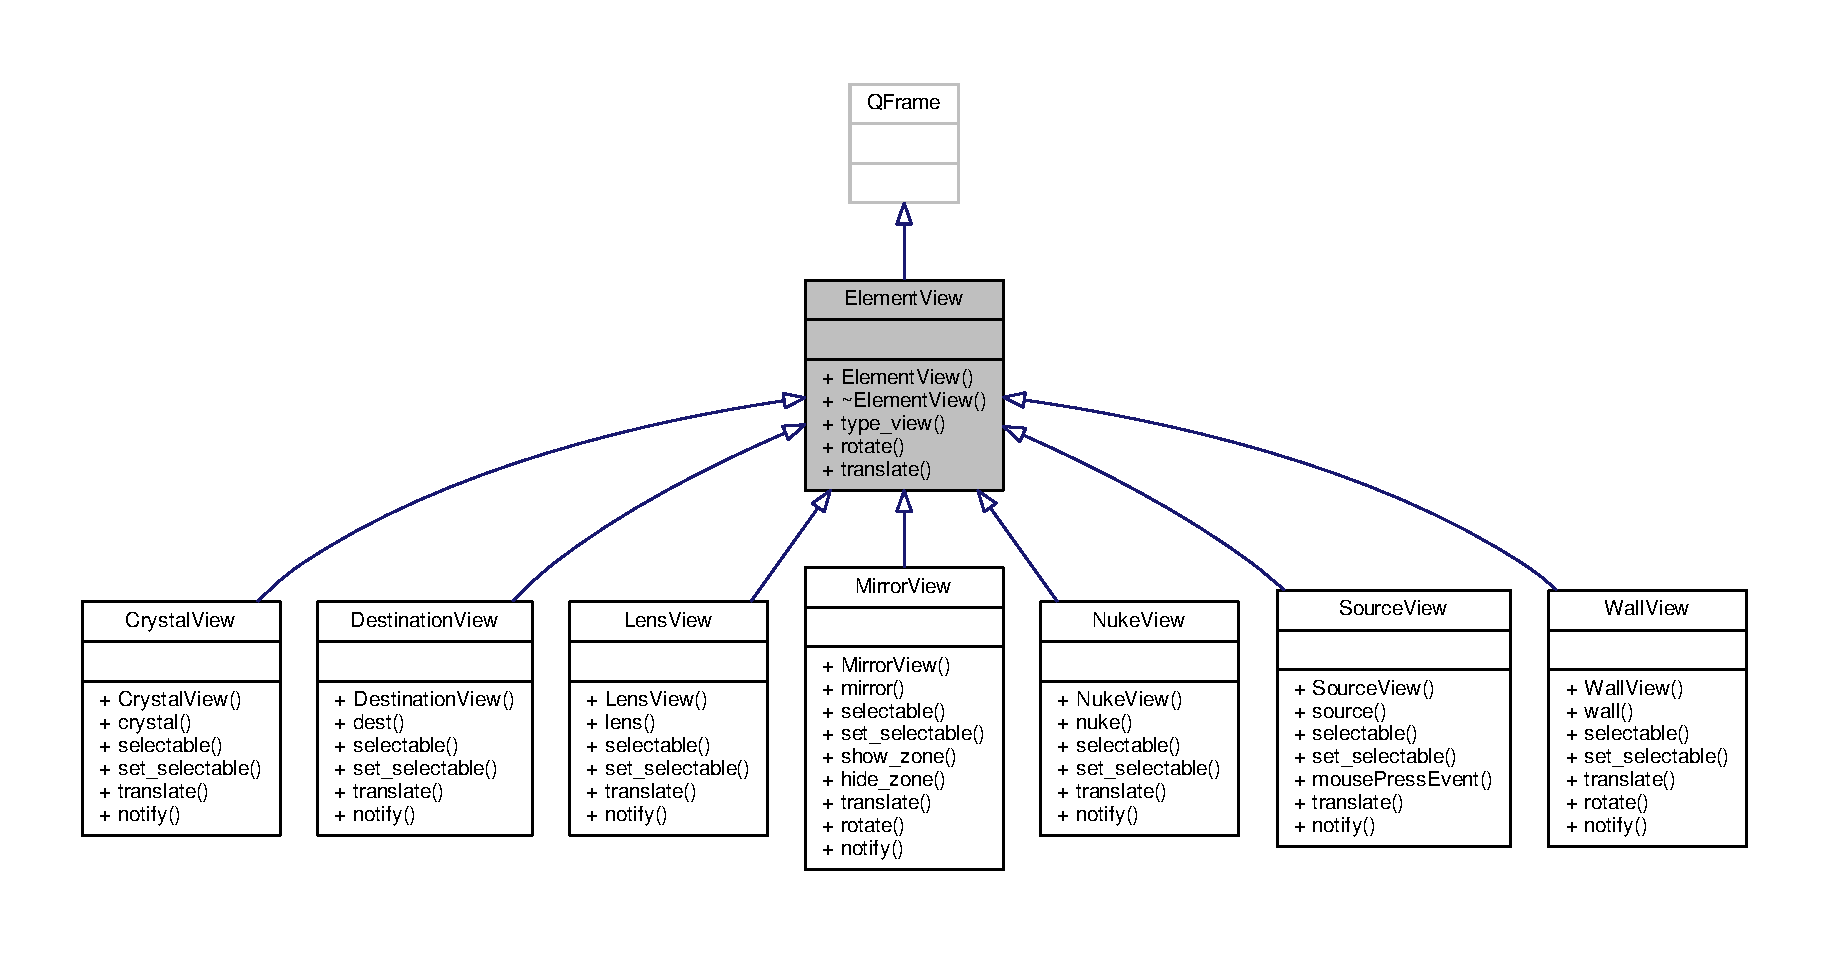
\includegraphics[width=350pt]{d8/d16/classElementView__inherit__graph}
\end{center}
\end{figure}


Graphe de collaboration de Element\+View\+:\nopagebreak
\begin{figure}[H]
\begin{center}
\leavevmode
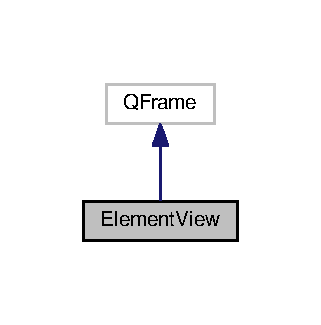
\includegraphics[width=154pt]{d3/d60/classElementView__coll__graph}
\end{center}
\end{figure}
\subsection*{Types publics}
\begin{DoxyCompactItemize}
\item 
\hypertarget{classElementView_ae8b9890c6c8501a7a759896cae9ab7a6}{enum {\bfseries Type\+View} \{ \\*
{\bfseries C\+R\+Y\+S\+T\+A\+L\+V\+I\+E\+W}, 
{\bfseries D\+E\+S\+T\+V\+I\+E\+W}, 
{\bfseries L\+E\+N\+S\+V\+I\+E\+W}, 
{\bfseries M\+I\+R\+R\+O\+R\+V\+I\+E\+W}, 
\\*
{\bfseries N\+U\+K\+E\+V\+I\+E\+W}, 
{\bfseries S\+O\+U\+R\+C\+E\+V\+I\+E\+W}, 
{\bfseries W\+A\+L\+L\+V\+I\+E\+W}
 \}}\label{classElementView_ae8b9890c6c8501a7a759896cae9ab7a6}

\end{DoxyCompactItemize}
\subsection*{Fonctions membres publiques}
\begin{DoxyCompactItemize}
\item 
\hypertarget{classElementView_adb918caf5a5fcc4bd945cd3cd2596f8c}{\hyperlink{classElementView_adb918caf5a5fcc4bd945cd3cd2596f8c}{Element\+View} (Element\+View\+::\+Type\+View)}\label{classElementView_adb918caf5a5fcc4bd945cd3cd2596f8c}

\begin{DoxyCompactList}\small\item\em Construit un élément avec un type permettant de connaître le type de l'élément à tout moment. \end{DoxyCompactList}\item 
const Type\+View \& \hyperlink{classElementView_a30b7a26b428be68dcc4d8f72a0f9cd0b}{type\+\_\+view} () const 
\begin{DoxyCompactList}\small\item\em Retourne le type de l'élément. \end{DoxyCompactList}\item 
virtual void \hyperlink{classElementView_a18589409290f23edffdaeccdd7acb015}{rotate} (const double r)
\begin{DoxyCompactList}\small\item\em Effectue une rotation d’un objet à l’aide d’un angle en radians. \end{DoxyCompactList}\item 
virtual void \hyperlink{classElementView_a69a525cb674a36e33be6a8b7a6e4b83c}{translate} (const double x, const double y)
\begin{DoxyCompactList}\small\item\em Effectue une translation de l’objet sur l’axe des abscisses et des ordonnées. \end{DoxyCompactList}\end{DoxyCompactItemize}


\subsection{Description détaillée}
Cette classe sert de super-\/classe à tous les éléments visuels avec lesquels un rayon peut interagir. 

Il s'agit plus d'une classe \char`\"{}\+T\+A\+G\char`\"{} pour retrouver le type d'un élément visuel. \begin{DoxySeeAlso}{Voir également}
\hyperlink{element_8h_source}{model/element.\+h} pour son équivalent modèle. 
\end{DoxySeeAlso}


\subsection{Documentation des fonctions membres}
\hypertarget{classElementView_a18589409290f23edffdaeccdd7acb015}{\index{Element\+View@{Element\+View}!rotate@{rotate}}
\index{rotate@{rotate}!Element\+View@{Element\+View}}
\subsubsection[{rotate}]{\setlength{\rightskip}{0pt plus 5cm}void Element\+View\+::rotate (
\begin{DoxyParamCaption}
\item[{const double}]{r}
\end{DoxyParamCaption}
)\hspace{0.3cm}{\ttfamily [virtual]}}}\label{classElementView_a18589409290f23edffdaeccdd7acb015}


Effectue une rotation d’un objet à l’aide d’un angle en radians. 


\begin{DoxyParams}{Paramètres}
{\em r} & angle en radian dont il faut faire pivoter l’objet. \\
\hline
\end{DoxyParams}


Réimplémentée dans \hyperlink{classMirrorView_aade5e65f7f7b4e0941bcaea616a60ac8}{Mirror\+View}, et \hyperlink{classWallView_a418bfa06482ecd61cd07533de32be0f1}{Wall\+View}.

\hypertarget{classElementView_a69a525cb674a36e33be6a8b7a6e4b83c}{\index{Element\+View@{Element\+View}!translate@{translate}}
\index{translate@{translate}!Element\+View@{Element\+View}}
\subsubsection[{translate}]{\setlength{\rightskip}{0pt plus 5cm}void Element\+View\+::translate (
\begin{DoxyParamCaption}
\item[{const double}]{x, }
\item[{const double}]{y}
\end{DoxyParamCaption}
)\hspace{0.3cm}{\ttfamily [virtual]}}}\label{classElementView_a69a525cb674a36e33be6a8b7a6e4b83c}


Effectue une translation de l’objet sur l’axe des abscisses et des ordonnées. 


\begin{DoxyParams}{Paramètres}
{\em x} & la translation sur l’axe des abscisses. \\
\hline
{\em y} & la translation sur l’axe des ordonnées. \\
\hline
\end{DoxyParams}


Réimplémentée dans \hyperlink{classCrystalView_a68f3f631351dce437a2c3ff86385e064}{Crystal\+View}, \hyperlink{classDestinationView_afd76d91b06a337ff123ad34af4fb25dd}{Destination\+View}, \hyperlink{classLensView_a9475ad917b91f93c23742f403ff152fc}{Lens\+View}, \hyperlink{classMirrorView_a4800c0c0ac2e7f7bfb3558f0f0dc25c2}{Mirror\+View}, \hyperlink{classSourceView_a96144eb5f08c6dc6b378fa604bb626a2}{Source\+View}, \hyperlink{classWallView_addb0495d120d6dfccd37cc0d65f32660}{Wall\+View}, et \hyperlink{classNukeView_ab5743729fc4659e2cd670d42800c9856}{Nuke\+View}.

\hypertarget{classElementView_a30b7a26b428be68dcc4d8f72a0f9cd0b}{\index{Element\+View@{Element\+View}!type\+\_\+view@{type\+\_\+view}}
\index{type\+\_\+view@{type\+\_\+view}!Element\+View@{Element\+View}}
\subsubsection[{type\+\_\+view}]{\setlength{\rightskip}{0pt plus 5cm}const Element\+View\+::\+Type\+View \& Element\+View\+::type\+\_\+view (
\begin{DoxyParamCaption}
{}
\end{DoxyParamCaption}
) const\hspace{0.3cm}{\ttfamily [inline]}}}\label{classElementView_a30b7a26b428be68dcc4d8f72a0f9cd0b}


Retourne le type de l'élément. 

\begin{DoxyReturn}{Renvoie}
le type de l'élément. 
\end{DoxyReturn}


La documentation de cette classe a été générée à partir des fichiers suivants \+:\begin{DoxyCompactItemize}
\item 
view/elementview.\+h\item 
view/elementview.\+cpp\end{DoxyCompactItemize}

\hypertarget{classEllipse}{\section{Référence de la classe Ellipse}
\label{classEllipse}\index{Ellipse@{Ellipse}}
}


Classe \hyperlink{classEllipse}{Ellipse} La position représente la position du centre de l'ellipse.  




{\ttfamily \#include $<$ellipse.\+h$>$}

\subsection*{Fonctions membres publiques}
\begin{DoxyCompactItemize}
\item 
\hyperlink{classEllipse_ad24260e249e5a78b67a779826e8e75d6}{Ellipse} (const \hyperlink{classPoint}{Point} \&p, double \hyperlink{classEllipse_a717ec722ed3528386b610b5ef6d560af}{x\+\_\+rad}, double \hyperlink{classEllipse_affc33b7f55133f772c94c8ae890fb5a0}{y\+\_\+rad})
\begin{DoxyCompactList}\small\item\em Crée une nouvelle ellipse. \end{DoxyCompactList}\item 
const \hyperlink{classPoint}{Point} \& \hyperlink{classEllipse_aab7c65b75ef01d20ec48f1e2b9308ebf}{center} () const 
\begin{DoxyCompactList}\small\item\em Retourne le point central de l'ellipse. \end{DoxyCompactList}\item 
double \hyperlink{classEllipse_a717ec722ed3528386b610b5ef6d560af}{x\+\_\+rad} () const 
\begin{DoxyCompactList}\small\item\em Retourne le rayon sur l'axe X. \end{DoxyCompactList}\item 
double \hyperlink{classEllipse_affc33b7f55133f772c94c8ae890fb5a0}{y\+\_\+rad} () const 
\begin{DoxyCompactList}\small\item\em Retourne le rayon sur l'axe Y. \end{DoxyCompactList}\end{DoxyCompactItemize}


\subsection{Description détaillée}
Classe \hyperlink{classEllipse}{Ellipse} La position représente la position du centre de l'ellipse. 

du rectangle entourant l'ellipse. Le x\+\_\+rad\+\_\+ correspond au rayon sur l'axe des X. Le y\+\_\+rad\+\_\+ correspond au rayon sur l'axe des Y. 

\subsection{Documentation des constructeurs et destructeur}
\hypertarget{classEllipse_ad24260e249e5a78b67a779826e8e75d6}{\index{Ellipse@{Ellipse}!Ellipse@{Ellipse}}
\index{Ellipse@{Ellipse}!Ellipse@{Ellipse}}
\subsubsection[{Ellipse}]{\setlength{\rightskip}{0pt plus 5cm}Ellipse\+::\+Ellipse (
\begin{DoxyParamCaption}
\item[{const {\bf Point} \&}]{p, }
\item[{double}]{x\+\_\+rad, }
\item[{double}]{y\+\_\+rad}
\end{DoxyParamCaption}
)}}\label{classEllipse_ad24260e249e5a78b67a779826e8e75d6}


Crée une nouvelle ellipse. 


\begin{DoxyParams}{Paramètres}
{\em p} & le coin supérieur gauche du rectangle entourant l'ellipse. \\
\hline
{\em x\+\_\+rad} & le rayon sur l'axe des X. \\
\hline
{\em y\+\_\+rad} & le rayon sur l'axe des Y. \\
\hline
\end{DoxyParams}


\subsection{Documentation des fonctions membres}
\hypertarget{classEllipse_aab7c65b75ef01d20ec48f1e2b9308ebf}{\index{Ellipse@{Ellipse}!center@{center}}
\index{center@{center}!Ellipse@{Ellipse}}
\subsubsection[{center}]{\setlength{\rightskip}{0pt plus 5cm}const {\bf Point} \& Ellipse\+::center (
\begin{DoxyParamCaption}
{}
\end{DoxyParamCaption}
) const\hspace{0.3cm}{\ttfamily [inline]}}}\label{classEllipse_aab7c65b75ef01d20ec48f1e2b9308ebf}


Retourne le point central de l'ellipse. 

\begin{DoxyReturn}{Renvoie}
le centre de l'ellipse. 
\end{DoxyReturn}
\hypertarget{classEllipse_a717ec722ed3528386b610b5ef6d560af}{\index{Ellipse@{Ellipse}!x\+\_\+rad@{x\+\_\+rad}}
\index{x\+\_\+rad@{x\+\_\+rad}!Ellipse@{Ellipse}}
\subsubsection[{x\+\_\+rad}]{\setlength{\rightskip}{0pt plus 5cm}double Ellipse\+::x\+\_\+rad (
\begin{DoxyParamCaption}
{}
\end{DoxyParamCaption}
) const\hspace{0.3cm}{\ttfamily [inline]}}}\label{classEllipse_a717ec722ed3528386b610b5ef6d560af}


Retourne le rayon sur l'axe X. 

\begin{DoxyReturn}{Renvoie}
le rayon sur l'axe X. 
\end{DoxyReturn}
\hypertarget{classEllipse_affc33b7f55133f772c94c8ae890fb5a0}{\index{Ellipse@{Ellipse}!y\+\_\+rad@{y\+\_\+rad}}
\index{y\+\_\+rad@{y\+\_\+rad}!Ellipse@{Ellipse}}
\subsubsection[{y\+\_\+rad}]{\setlength{\rightskip}{0pt plus 5cm}double Ellipse\+::y\+\_\+rad (
\begin{DoxyParamCaption}
{}
\end{DoxyParamCaption}
) const\hspace{0.3cm}{\ttfamily [inline]}}}\label{classEllipse_affc33b7f55133f772c94c8ae890fb5a0}


Retourne le rayon sur l'axe Y. 

\begin{DoxyReturn}{Renvoie}
le rayon sur l'axe Y. 
\end{DoxyReturn}


La documentation de cette classe a été générée à partir des fichiers suivants \+:\begin{DoxyCompactItemize}
\item 
model/ellipse.\+h\item 
model/ellipse.\+cpp\end{DoxyCompactItemize}

\hypertarget{structIntersection}{\section{Référence de la structure Intersection}
\label{structIntersection}\index{Intersection@{Intersection}}
}


Structure intersection \+: Possède un élément et un point d'intersection.  




{\ttfamily \#include $<$level.\+h$>$}



Graphe de collaboration de Intersection\+:\nopagebreak
\begin{figure}[H]
\begin{center}
\leavevmode
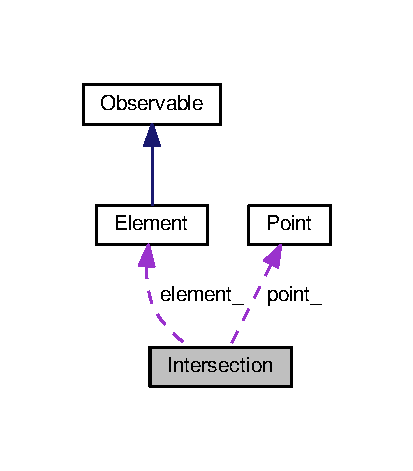
\includegraphics[width=198pt]{d9/d8e/structIntersection__coll__graph}
\end{center}
\end{figure}
\subsection*{Fonctions membres publiques}
\begin{DoxyCompactItemize}
\item 
\hyperlink{structIntersection_a44d7ebd733fe15894a44f14a63c3d328}{Intersection} (\hyperlink{classPoint}{Point} $\ast$p, \hyperlink{classElement}{Element} $\ast$e)
\begin{DoxyCompactList}\small\item\em Crée une nouvelle intersection. \end{DoxyCompactList}\end{DoxyCompactItemize}
\subsection*{Attributs publics}
\begin{DoxyCompactItemize}
\item 
\hypertarget{structIntersection_ac914f236feced83128e4f542d21327b2}{\hyperlink{classPoint}{Point} $\ast$ {\bfseries point\+\_\+}}\label{structIntersection_ac914f236feced83128e4f542d21327b2}

\item 
\hypertarget{structIntersection_aae28864f0cb6a95503384a73c33ad4cd}{\hyperlink{classElement}{Element} $\ast$ {\bfseries element\+\_\+}}\label{structIntersection_aae28864f0cb6a95503384a73c33ad4cd}

\end{DoxyCompactItemize}


\subsection{Description détaillée}
Structure intersection \+: Possède un élément et un point d'intersection. 

\subsection{Documentation des constructeurs et destructeur}
\hypertarget{structIntersection_a44d7ebd733fe15894a44f14a63c3d328}{\index{Intersection@{Intersection}!Intersection@{Intersection}}
\index{Intersection@{Intersection}!Intersection@{Intersection}}
\subsubsection[{Intersection}]{\setlength{\rightskip}{0pt plus 5cm}Intersection\+::\+Intersection (
\begin{DoxyParamCaption}
\item[{{\bf Point} $\ast$}]{p, }
\item[{{\bf Element} $\ast$}]{e}
\end{DoxyParamCaption}
)\hspace{0.3cm}{\ttfamily [inline]}}}\label{structIntersection_a44d7ebd733fe15894a44f14a63c3d328}


Crée une nouvelle intersection. 


\begin{DoxyParams}{Paramètres}
{\em p} & le point d'intersection. \\
\hline
{\em e} & l'élément de l'intersection. \\
\hline
\end{DoxyParams}


La documentation de cette structure a été générée à partir du fichier suivant \+:\begin{DoxyCompactItemize}
\item 
model/level.\+h\end{DoxyCompactItemize}

\hypertarget{classLens}{\section{Référence de la classe Lens}
\label{classLens}\index{Lens@{Lens}}
}


Cette classe modélise les lentilles utilisées dans le jeu.  




{\ttfamily \#include $<$lens.\+h$>$}



Graphe d'héritage de Lens\+:
\nopagebreak
\begin{figure}[H]
\begin{center}
\leavevmode
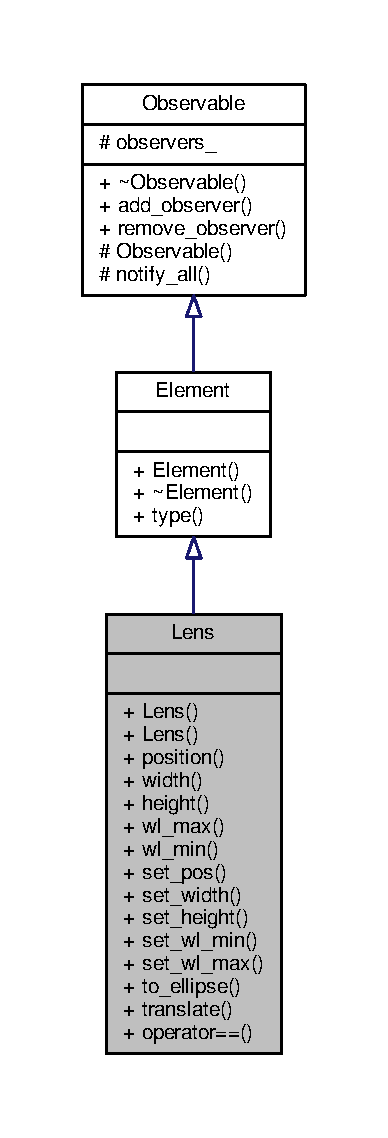
\includegraphics[width=186pt]{d4/def/classLens__inherit__graph}
\end{center}
\end{figure}


Graphe de collaboration de Lens\+:
\nopagebreak
\begin{figure}[H]
\begin{center}
\leavevmode
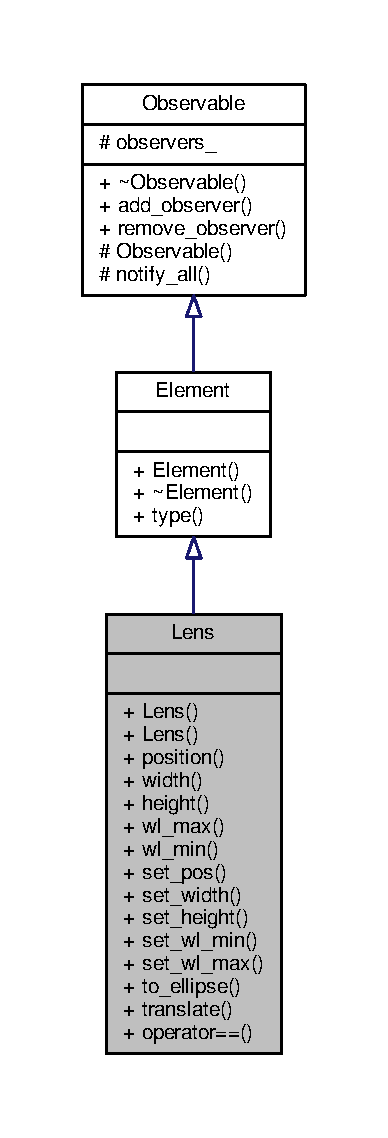
\includegraphics[width=186pt]{d8/df0/classLens__coll__graph}
\end{center}
\end{figure}
\subsection*{Fonctions membres publiques}
\begin{DoxyCompactItemize}
\item 
\hyperlink{classLens_a314445802fc5ed95bdd6b715282f6825}{Lens} (const \hyperlink{classPoint}{Point} \&p, double w, double h, int \hyperlink{classLens_aee260137e02f65dd1e3daf3ce21a85c2}{wl\+\_\+min}, int \hyperlink{classLens_a0ffa3d4a046dd6d31ddc549bd91bc25d}{wl\+\_\+max})
\begin{DoxyCompactList}\small\item\em Instancie une lentille à l'aide de toutes ses caractéristiques. \end{DoxyCompactList}\item 
\hyperlink{classLens_a3912f09431d56887039ae7feaf1fa169}{Lens} (const \hyperlink{classLens}{Lens} \&lens)
\begin{DoxyCompactList}\small\item\em Constructeur de copie. \end{DoxyCompactList}\item 
const \hyperlink{classPoint}{Point} \& \hyperlink{classLens_a162d1b06824dbbac8c221ebfec0e0816}{position} () const 
\begin{DoxyCompactList}\small\item\em Retourne la position du coin supérieur gauche du rectangle modélisant la lentille. \end{DoxyCompactList}\item 
double \hyperlink{classLens_afcccf7e103a81ae4fbe5e14c9dc4e0a6}{width} () const 
\begin{DoxyCompactList}\small\item\em Retourne la largeur de la lentille. \end{DoxyCompactList}\item 
double \hyperlink{classLens_a827d7ce14d1dfbd66b46e94cb1d6a794}{height} () const 
\begin{DoxyCompactList}\small\item\em Retourne la hauteur de la lentille. \end{DoxyCompactList}\item 
int \hyperlink{classLens_a0ffa3d4a046dd6d31ddc549bd91bc25d}{wl\+\_\+max} () const 
\begin{DoxyCompactList}\small\item\em Retourne la longueur d'onde minimale des rayons autorisés à franchir la lentille. \end{DoxyCompactList}\item 
int \hyperlink{classLens_aee260137e02f65dd1e3daf3ce21a85c2}{wl\+\_\+min} () const 
\begin{DoxyCompactList}\small\item\em Retourne la longueur d'onde maximale des rayons autorisés à franchir la lentille. \end{DoxyCompactList}\item 
void \hyperlink{classLens_a3bf3faa62c56d0282e46c2f0baa3b531}{set\+\_\+pos} (const \hyperlink{classPoint}{Point} \&pos)
\begin{DoxyCompactList}\small\item\em Modifie la position de la lentille. \end{DoxyCompactList}\item 
void \hyperlink{classLens_a7667bda90f872998cb19a027d1c4f3db}{set\+\_\+width} (const double w)
\begin{DoxyCompactList}\small\item\em Modifie la largeur de la lentille. \end{DoxyCompactList}\item 
void \hyperlink{classLens_a8242b785736433197468c6ef17fb37ee}{set\+\_\+height} (const double h)
\begin{DoxyCompactList}\small\item\em Modifie la hauteur de la lentille. \end{DoxyCompactList}\item 
void \hyperlink{classLens_a0fedf88bbe8eb0bdb4a5d20561f1344c}{set\+\_\+wl\+\_\+min} (const double \hyperlink{classLens_aee260137e02f65dd1e3daf3ce21a85c2}{wl\+\_\+min})
\begin{DoxyCompactList}\small\item\em Modifie la longueur d’onde minimale de la lentille. \end{DoxyCompactList}\item 
void \hyperlink{classLens_a7c0492c65283b7f51f54aef6c706d311}{set\+\_\+wl\+\_\+max} (const double \hyperlink{classLens_a0ffa3d4a046dd6d31ddc549bd91bc25d}{wl\+\_\+max})
\begin{DoxyCompactList}\small\item\em Modifie la longueur d’onde maximale de la lentille. \end{DoxyCompactList}\item 
\hyperlink{classEllipse}{Ellipse} \hyperlink{classLens_a32c53f8267002b2fa510c656f91600b9}{to\+\_\+ellipse} ()
\begin{DoxyCompactList}\small\item\em Retourne une ellipse correspondante à la lentille. \end{DoxyCompactList}\item 
void \hyperlink{classLens_acfdbf14808b0c555e21405aacd7d9cb2}{translate} (const double x, const double y)
\begin{DoxyCompactList}\small\item\em Déplace la lentille. \end{DoxyCompactList}\item 
bool \hyperlink{classLens_a53256728d15126197e0f66a595822948}{operator==} (const \hyperlink{classLens}{Lens} \&l) const 
\begin{DoxyCompactList}\small\item\em Redéfinition de l'opérateur d'égalité, retourne vrai si les lentilles sont égales. \end{DoxyCompactList}\end{DoxyCompactItemize}
\subsection*{Amis}
\begin{DoxyCompactItemize}
\item 
std\+::ostream \& \hyperlink{classLens_ad6aeaa87264bd2229fef327ef4c64699}{operator$<$$<$} (std\+::ostream \&out, const \hyperlink{classLens}{Lens} \&m)
\begin{DoxyCompactList}\small\item\em Surcharge l'opérateur de flux de sortie pour afficher un récapitulatif des caractéristiques de la lentille sous-\/jacente en console. \end{DoxyCompactList}\end{DoxyCompactItemize}
\subsection*{Membres hérités additionnels}


\subsection{Description détaillée}
Cette classe modélise les lentilles utilisées dans le jeu. 

Une lentille est un objet rectangulaire qui ne laisse passer les rayons lumineux que dans un certain intervalle de longueur d'onde. Si un rayon lumineux se trouve dans l'intervalle de longueur d'onde autorisé, il traverse la lentille sans subir aucune modification. Sinon, la lentille se comporte comme un mur. 

\subsection{Documentation des constructeurs et destructeur}
\hypertarget{classLens_a314445802fc5ed95bdd6b715282f6825}{\index{Lens@{Lens}!Lens@{Lens}}
\index{Lens@{Lens}!Lens@{Lens}}
\subsubsection[{Lens}]{\setlength{\rightskip}{0pt plus 5cm}Lens\+::\+Lens (
\begin{DoxyParamCaption}
\item[{const {\bf Point} \&}]{p, }
\item[{double}]{w, }
\item[{double}]{h, }
\item[{int}]{wl\+\_\+min, }
\item[{int}]{wl\+\_\+max}
\end{DoxyParamCaption}
)}}\label{classLens_a314445802fc5ed95bdd6b715282f6825}


Instancie une lentille à l'aide de toutes ses caractéristiques. 


\begin{DoxyParams}{Paramètres}
{\em p} & la position du coin supérieur gauche du rectangle modélisant la lentille. \\
\hline
{\em w} & la largeur de la lentille. \\
\hline
{\em h} & la hauteur de la lentille. \\
\hline
{\em wl\+\_\+min} & la longueur d'onde minimale des rayons autorisés à franchir la lentille. \\
\hline
{\em wl\+\_\+max} & la longueur d'onde maximale des rayons autorisés à franchir la lentille. \\
\hline
\end{DoxyParams}
\hypertarget{classLens_a3912f09431d56887039ae7feaf1fa169}{\index{Lens@{Lens}!Lens@{Lens}}
\index{Lens@{Lens}!Lens@{Lens}}
\subsubsection[{Lens}]{\setlength{\rightskip}{0pt plus 5cm}Lens\+::\+Lens (
\begin{DoxyParamCaption}
\item[{const {\bf Lens} \&}]{lens}
\end{DoxyParamCaption}
)}}\label{classLens_a3912f09431d56887039ae7feaf1fa169}


Constructeur de copie. 


\begin{DoxyParams}{Paramètres}
{\em lens} & la lentille à copier. \\
\hline
\end{DoxyParams}


\subsection{Documentation des fonctions membres}
\hypertarget{classLens_a827d7ce14d1dfbd66b46e94cb1d6a794}{\index{Lens@{Lens}!height@{height}}
\index{height@{height}!Lens@{Lens}}
\subsubsection[{height}]{\setlength{\rightskip}{0pt plus 5cm}double Lens\+::height (
\begin{DoxyParamCaption}
{}
\end{DoxyParamCaption}
) const\hspace{0.3cm}{\ttfamily [inline]}}}\label{classLens_a827d7ce14d1dfbd66b46e94cb1d6a794}


Retourne la hauteur de la lentille. 

\begin{DoxyReturn}{Renvoie}
la hauteur de la lentille. 
\end{DoxyReturn}
\hypertarget{classLens_a53256728d15126197e0f66a595822948}{\index{Lens@{Lens}!operator==@{operator==}}
\index{operator==@{operator==}!Lens@{Lens}}
\subsubsection[{operator==}]{\setlength{\rightskip}{0pt plus 5cm}bool Lens\+::operator== (
\begin{DoxyParamCaption}
\item[{const {\bf Lens} \&}]{l}
\end{DoxyParamCaption}
) const}}\label{classLens_a53256728d15126197e0f66a595822948}


Redéfinition de l'opérateur d'égalité, retourne vrai si les lentilles sont égales. 


\begin{DoxyParams}{Paramètres}
{\em l} & une lentille. \\
\hline
\end{DoxyParams}
\begin{DoxyReturn}{Renvoie}
vrai si les lentilles sont égales, faux sinon. 
\end{DoxyReturn}
\hypertarget{classLens_a162d1b06824dbbac8c221ebfec0e0816}{\index{Lens@{Lens}!position@{position}}
\index{position@{position}!Lens@{Lens}}
\subsubsection[{position}]{\setlength{\rightskip}{0pt plus 5cm}const {\bf Point} \& Lens\+::position (
\begin{DoxyParamCaption}
{}
\end{DoxyParamCaption}
) const\hspace{0.3cm}{\ttfamily [inline]}}}\label{classLens_a162d1b06824dbbac8c221ebfec0e0816}


Retourne la position du coin supérieur gauche du rectangle modélisant la lentille. 

\begin{DoxyReturn}{Renvoie}
la position du coin supérieur gauche du rectangle modélisant la lentille 
\end{DoxyReturn}
\hypertarget{classLens_a8242b785736433197468c6ef17fb37ee}{\index{Lens@{Lens}!set\+\_\+height@{set\+\_\+height}}
\index{set\+\_\+height@{set\+\_\+height}!Lens@{Lens}}
\subsubsection[{set\+\_\+height}]{\setlength{\rightskip}{0pt plus 5cm}void Lens\+::set\+\_\+height (
\begin{DoxyParamCaption}
\item[{const double}]{h}
\end{DoxyParamCaption}
)\hspace{0.3cm}{\ttfamily [inline]}}}\label{classLens_a8242b785736433197468c6ef17fb37ee}


Modifie la hauteur de la lentille. 


\begin{DoxyParams}{Paramètres}
{\em h} & la nouvelle hauteur de la lentille. \\
\hline
\end{DoxyParams}
\hypertarget{classLens_a3bf3faa62c56d0282e46c2f0baa3b531}{\index{Lens@{Lens}!set\+\_\+pos@{set\+\_\+pos}}
\index{set\+\_\+pos@{set\+\_\+pos}!Lens@{Lens}}
\subsubsection[{set\+\_\+pos}]{\setlength{\rightskip}{0pt plus 5cm}void Lens\+::set\+\_\+pos (
\begin{DoxyParamCaption}
\item[{const {\bf Point} \&}]{pos}
\end{DoxyParamCaption}
)\hspace{0.3cm}{\ttfamily [inline]}}}\label{classLens_a3bf3faa62c56d0282e46c2f0baa3b531}


Modifie la position de la lentille. 


\begin{DoxyParams}{Paramètres}
{\em pos} & la nouvelle position de la lentille. \\
\hline
\end{DoxyParams}
\hypertarget{classLens_a7667bda90f872998cb19a027d1c4f3db}{\index{Lens@{Lens}!set\+\_\+width@{set\+\_\+width}}
\index{set\+\_\+width@{set\+\_\+width}!Lens@{Lens}}
\subsubsection[{set\+\_\+width}]{\setlength{\rightskip}{0pt plus 5cm}void Lens\+::set\+\_\+width (
\begin{DoxyParamCaption}
\item[{const double}]{w}
\end{DoxyParamCaption}
)\hspace{0.3cm}{\ttfamily [inline]}}}\label{classLens_a7667bda90f872998cb19a027d1c4f3db}


Modifie la largeur de la lentille. 


\begin{DoxyParams}{Paramètres}
{\em w} & la nouvelle largeur de la lentille. \\
\hline
\end{DoxyParams}
\hypertarget{classLens_a7c0492c65283b7f51f54aef6c706d311}{\index{Lens@{Lens}!set\+\_\+wl\+\_\+max@{set\+\_\+wl\+\_\+max}}
\index{set\+\_\+wl\+\_\+max@{set\+\_\+wl\+\_\+max}!Lens@{Lens}}
\subsubsection[{set\+\_\+wl\+\_\+max}]{\setlength{\rightskip}{0pt plus 5cm}void Lens\+::set\+\_\+wl\+\_\+max (
\begin{DoxyParamCaption}
\item[{const double}]{wl\+\_\+max}
\end{DoxyParamCaption}
)\hspace{0.3cm}{\ttfamily [inline]}}}\label{classLens_a7c0492c65283b7f51f54aef6c706d311}


Modifie la longueur d’onde maximale de la lentille. 


\begin{DoxyParams}{Paramètres}
{\em wl\+\_\+max} & la nouvelle longueur d’onde maximale. \\
\hline
\end{DoxyParams}
\hypertarget{classLens_a0fedf88bbe8eb0bdb4a5d20561f1344c}{\index{Lens@{Lens}!set\+\_\+wl\+\_\+min@{set\+\_\+wl\+\_\+min}}
\index{set\+\_\+wl\+\_\+min@{set\+\_\+wl\+\_\+min}!Lens@{Lens}}
\subsubsection[{set\+\_\+wl\+\_\+min}]{\setlength{\rightskip}{0pt plus 5cm}void Lens\+::set\+\_\+wl\+\_\+min (
\begin{DoxyParamCaption}
\item[{const double}]{wl\+\_\+min}
\end{DoxyParamCaption}
)\hspace{0.3cm}{\ttfamily [inline]}}}\label{classLens_a0fedf88bbe8eb0bdb4a5d20561f1344c}


Modifie la longueur d’onde minimale de la lentille. 


\begin{DoxyParams}{Paramètres}
{\em wl\+\_\+min} & la nouvelle longueur d’onde minimale. \\
\hline
\end{DoxyParams}
\hypertarget{classLens_a32c53f8267002b2fa510c656f91600b9}{\index{Lens@{Lens}!to\+\_\+ellipse@{to\+\_\+ellipse}}
\index{to\+\_\+ellipse@{to\+\_\+ellipse}!Lens@{Lens}}
\subsubsection[{to\+\_\+ellipse}]{\setlength{\rightskip}{0pt plus 5cm}{\bf Ellipse} Lens\+::to\+\_\+ellipse (
\begin{DoxyParamCaption}
{}
\end{DoxyParamCaption}
)}}\label{classLens_a32c53f8267002b2fa510c656f91600b9}


Retourne une ellipse correspondante à la lentille. 

\begin{DoxyReturn}{Renvoie}
l'ellipse correspondante à la lentille. 
\end{DoxyReturn}
\hypertarget{classLens_acfdbf14808b0c555e21405aacd7d9cb2}{\index{Lens@{Lens}!translate@{translate}}
\index{translate@{translate}!Lens@{Lens}}
\subsubsection[{translate}]{\setlength{\rightskip}{0pt plus 5cm}void Lens\+::translate (
\begin{DoxyParamCaption}
\item[{const double}]{x, }
\item[{const double}]{y}
\end{DoxyParamCaption}
)}}\label{classLens_acfdbf14808b0c555e21405aacd7d9cb2}


Déplace la lentille. 


\begin{DoxyParams}{Paramètres}
{\em x} & le déplacement sur l'axe x. \\
\hline
{\em y} & le déplacement sur l'axe y. \\
\hline
\end{DoxyParams}
\hypertarget{classLens_afcccf7e103a81ae4fbe5e14c9dc4e0a6}{\index{Lens@{Lens}!width@{width}}
\index{width@{width}!Lens@{Lens}}
\subsubsection[{width}]{\setlength{\rightskip}{0pt plus 5cm}double Lens\+::width (
\begin{DoxyParamCaption}
{}
\end{DoxyParamCaption}
) const\hspace{0.3cm}{\ttfamily [inline]}}}\label{classLens_afcccf7e103a81ae4fbe5e14c9dc4e0a6}


Retourne la largeur de la lentille. 

\begin{DoxyReturn}{Renvoie}
la largeur de la lentille. 
\end{DoxyReturn}
\hypertarget{classLens_a0ffa3d4a046dd6d31ddc549bd91bc25d}{\index{Lens@{Lens}!wl\+\_\+max@{wl\+\_\+max}}
\index{wl\+\_\+max@{wl\+\_\+max}!Lens@{Lens}}
\subsubsection[{wl\+\_\+max}]{\setlength{\rightskip}{0pt plus 5cm}int Lens\+::wl\+\_\+max (
\begin{DoxyParamCaption}
{}
\end{DoxyParamCaption}
) const\hspace{0.3cm}{\ttfamily [inline]}}}\label{classLens_a0ffa3d4a046dd6d31ddc549bd91bc25d}


Retourne la longueur d'onde minimale des rayons autorisés à franchir la lentille. 

\begin{DoxyReturn}{Renvoie}
la longueur d'onde minimale des rayons autorisés à franchir la lentille. 
\end{DoxyReturn}
\hypertarget{classLens_aee260137e02f65dd1e3daf3ce21a85c2}{\index{Lens@{Lens}!wl\+\_\+min@{wl\+\_\+min}}
\index{wl\+\_\+min@{wl\+\_\+min}!Lens@{Lens}}
\subsubsection[{wl\+\_\+min}]{\setlength{\rightskip}{0pt plus 5cm}int Lens\+::wl\+\_\+min (
\begin{DoxyParamCaption}
{}
\end{DoxyParamCaption}
) const\hspace{0.3cm}{\ttfamily [inline]}}}\label{classLens_aee260137e02f65dd1e3daf3ce21a85c2}


Retourne la longueur d'onde maximale des rayons autorisés à franchir la lentille. 

\begin{DoxyReturn}{Renvoie}
la longueur d'onde maximale des rayons autorisés à franchir la lentille. 
\end{DoxyReturn}


\subsection{Documentation des fonctions amies et associées}
\hypertarget{classLens_ad6aeaa87264bd2229fef327ef4c64699}{\index{Lens@{Lens}!operator$<$$<$@{operator$<$$<$}}
\index{operator$<$$<$@{operator$<$$<$}!Lens@{Lens}}
\subsubsection[{operator$<$$<$}]{\setlength{\rightskip}{0pt plus 5cm}std\+::ostream\& operator$<$$<$ (
\begin{DoxyParamCaption}
\item[{std\+::ostream \&}]{out, }
\item[{const {\bf Lens} \&}]{m}
\end{DoxyParamCaption}
)\hspace{0.3cm}{\ttfamily [friend]}}}\label{classLens_ad6aeaa87264bd2229fef327ef4c64699}


Surcharge l'opérateur de flux de sortie pour afficher un récapitulatif des caractéristiques de la lentille sous-\/jacente en console. 

\begin{DoxyReturn}{Renvoie}
le flux dans lequel la lentille a été imprimée. 
\end{DoxyReturn}


La documentation de cette classe a été générée à partir des fichiers suivants \+:\begin{DoxyCompactItemize}
\item 
model/lens.\+h\item 
model/lens.\+cpp\end{DoxyCompactItemize}

\hypertarget{classLensProp}{\section{Référence de la classe Lens\+Prop}
\label{classLensProp}\index{Lens\+Prop@{Lens\+Prop}}
}


Graphe d'héritage de Lens\+Prop\+:
\nopagebreak
\begin{figure}[H]
\begin{center}
\leavevmode
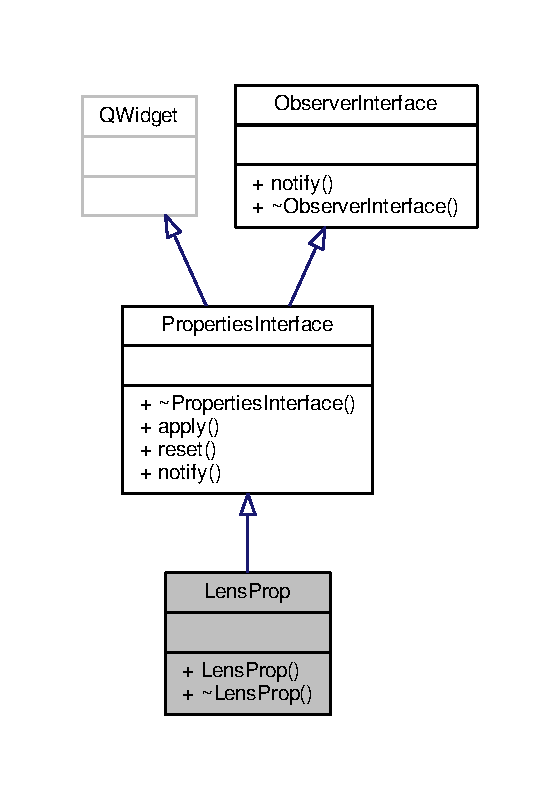
\includegraphics[width=247pt]{d8/d9c/classLensProp__inherit__graph}
\end{center}
\end{figure}


Graphe de collaboration de Lens\+Prop\+:
\nopagebreak
\begin{figure}[H]
\begin{center}
\leavevmode
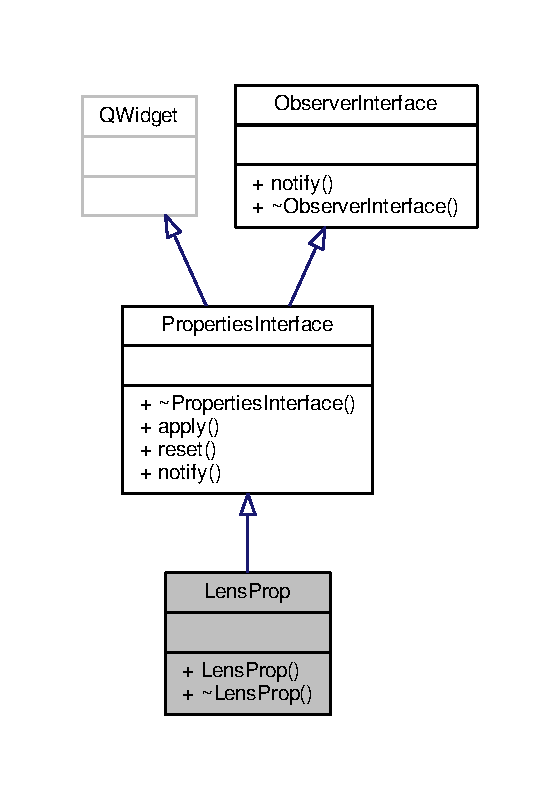
\includegraphics[width=247pt]{de/d14/classLensProp__coll__graph}
\end{center}
\end{figure}
\subsection*{Fonctions membres publiques}
\begin{DoxyCompactItemize}
\item 
\hypertarget{classLensProp_a2a9f54d768d72f8ad69e1572259d2a85}{{\bfseries Lens\+Prop} (\hyperlink{classLens}{Lens} $\ast$lens, Q\+Widget $\ast$parent=0)}\label{classLensProp_a2a9f54d768d72f8ad69e1572259d2a85}

\item 
\hypertarget{classLensProp_a4b21de75fded3126b60dd75e17811e97}{void {\bfseries setup\+Ui} ()}\label{classLensProp_a4b21de75fded3126b60dd75e17811e97}

\end{DoxyCompactItemize}


La documentation de cette classe a été générée à partir des fichiers suivants \+:\begin{DoxyCompactItemize}
\item 
editor/lensprop.\+h\item 
editor/lensprop.\+cpp\end{DoxyCompactItemize}

\hypertarget{classLensView}{\section{Référence de la classe Lens\+View}
\label{classLensView}\index{Lens\+View@{Lens\+View}}
}


Graphe d'héritage de Lens\+View\+:\nopagebreak
\begin{figure}[H]
\begin{center}
\leavevmode
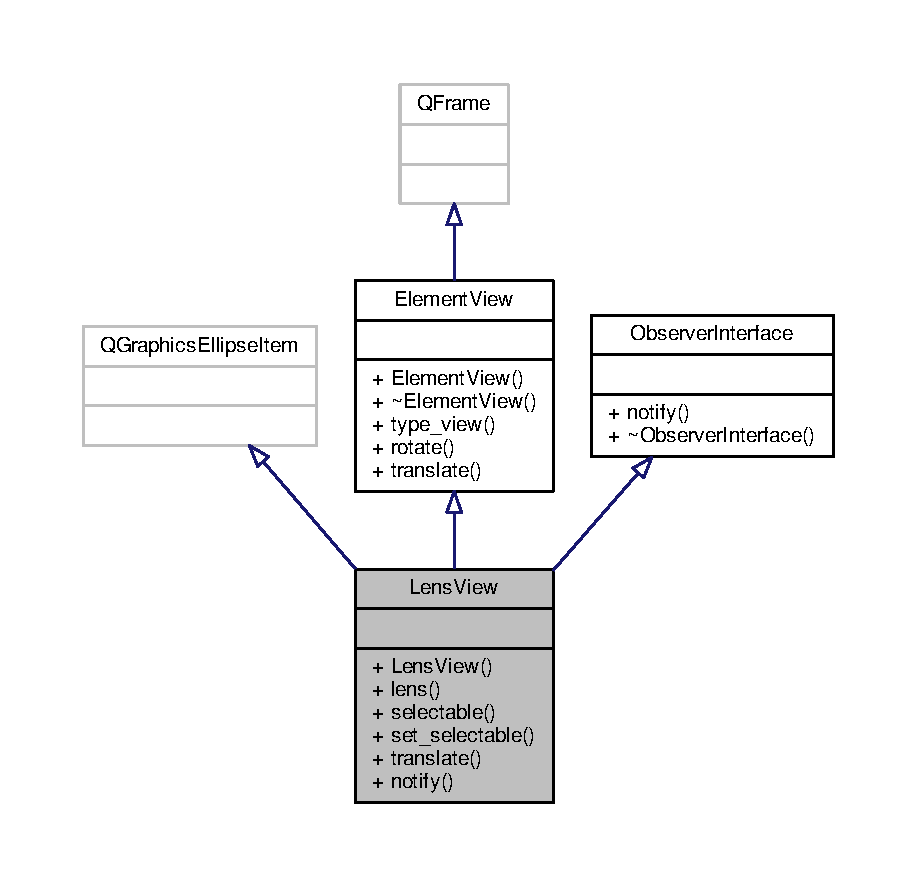
\includegraphics[width=350pt]{d3/d0e/classLensView__inherit__graph}
\end{center}
\end{figure}


Graphe de collaboration de Lens\+View\+:\nopagebreak
\begin{figure}[H]
\begin{center}
\leavevmode
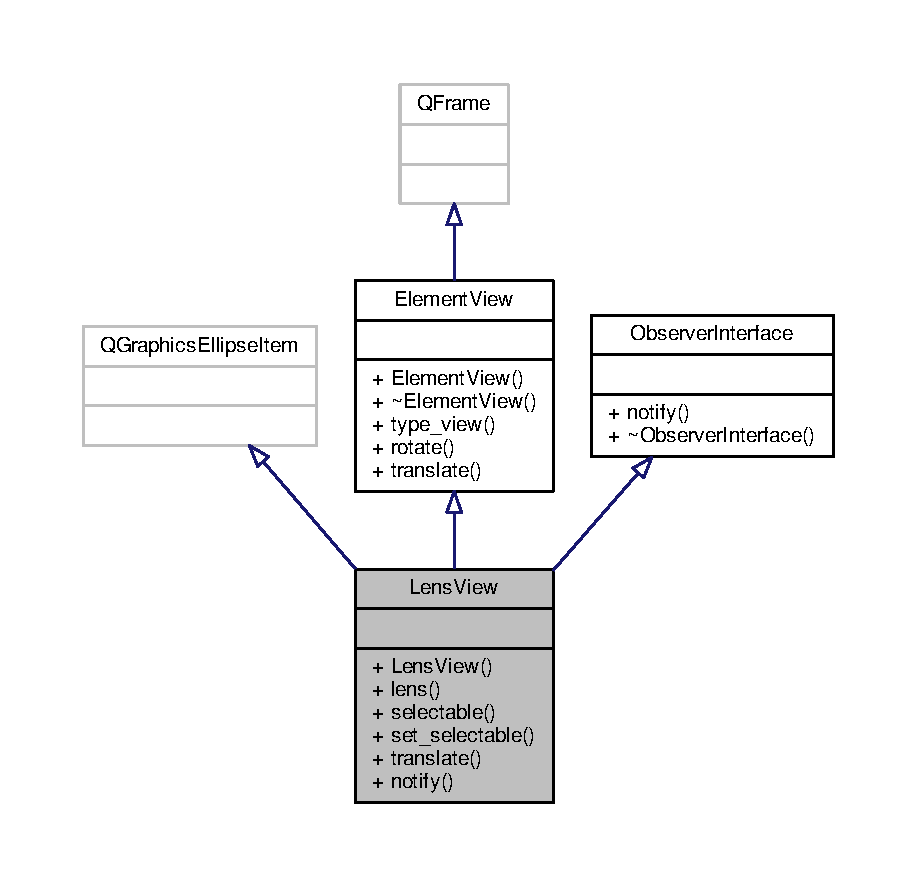
\includegraphics[width=350pt]{d3/d32/classLensView__coll__graph}
\end{center}
\end{figure}
\subsection*{Fonctions membres publiques}
\begin{DoxyCompactItemize}
\item 
\hypertarget{classLensView_a678ca25c84417e53af04258d27e5979a}{{\bfseries Lens\+View} (const \hyperlink{classLens}{Lens} \&lens, bool selectable=false)}\label{classLensView_a678ca25c84417e53af04258d27e5979a}

\item 
\hypertarget{classLensView_a9af15abae80b9588e61de5a0d929101f}{\hyperlink{classLens}{Lens} $\ast$ {\bfseries lens} ()}\label{classLensView_a9af15abae80b9588e61de5a0d929101f}

\item 
\hypertarget{classLensView_abcf4b929c4008fe2d0d464e1ec113037}{bool {\bfseries selectable} () const }\label{classLensView_abcf4b929c4008fe2d0d464e1ec113037}

\item 
\hypertarget{classLensView_a3a35c1e61503da599b1d9c93c176dffd}{void {\bfseries set\+\_\+selectable} (bool value)}\label{classLensView_a3a35c1e61503da599b1d9c93c176dffd}

\item 
\hypertarget{classLensView_a60a6a9fa6212d8d5997c77f8ee63b38d}{void {\bfseries translate} (double x=.\+0, double y=.\+0)}\label{classLensView_a60a6a9fa6212d8d5997c77f8ee63b38d}

\item 
void \hyperlink{classLensView_a55574a71ccc10e389b155b4029f74d5a}{notify} (\hyperlink{classObservable}{Observable} $\ast$sdo, std\+::string msg, const std\+::vector$<$ std\+::string $>$ \&args=std\+::vector$<$ std\+::string $>$())
\begin{DoxyCompactList}\small\item\em Notifie le jeu d'un évènement provenant d'un sujet d'observation (\hyperlink{classObservable}{Observable}). \end{DoxyCompactList}\end{DoxyCompactItemize}
\subsection*{Membres hérités additionnels}


\subsection{Documentation des fonctions membres}
\hypertarget{classLensView_a55574a71ccc10e389b155b4029f74d5a}{\index{Lens\+View@{Lens\+View}!notify@{notify}}
\index{notify@{notify}!Lens\+View@{Lens\+View}}
\subsubsection[{notify}]{\setlength{\rightskip}{0pt plus 5cm}void Lens\+View\+::notify (
\begin{DoxyParamCaption}
\item[{{\bf Observable} $\ast$}]{sdo, }
\item[{std\+::string}]{msg, }
\item[{const std\+::vector$<$ std\+::string $>$ \&}]{args = {\ttfamily std\+:\+:vector$<$~std\+:\+:string~$>$()}}
\end{DoxyParamCaption}
)\hspace{0.3cm}{\ttfamily [virtual]}}}\label{classLensView_a55574a71ccc10e389b155b4029f74d5a}


Notifie le jeu d'un évènement provenant d'un sujet d'observation (\hyperlink{classObservable}{Observable}). 


\begin{DoxyParams}{Paramètres}
{\em o} & l'observé. \\
\hline
{\em msg} & le message de notification. \\
\hline
{\em args} & des arguments. \\
\hline
\end{DoxyParams}


Implémente \hyperlink{classObserverInterface_a1bbd22519c2942d978804714db12c8b2}{Observer\+Interface}.



La documentation de cette classe a été générée à partir des fichiers suivants \+:\begin{DoxyCompactItemize}
\item 
view/lensview.\+h\item 
view/lensview.\+cpp\end{DoxyCompactItemize}

\hypertarget{classLevel}{\section{Référence de la classe Level}
\label{classLevel}\index{Level@{Level}}
}


Modélise une carte telle qu'utilisée dans le jeu.  




{\ttfamily \#include $<$level.\+h$>$}



Graphe d'héritage de Level\+:
\nopagebreak
\begin{figure}[H]
\begin{center}
\leavevmode
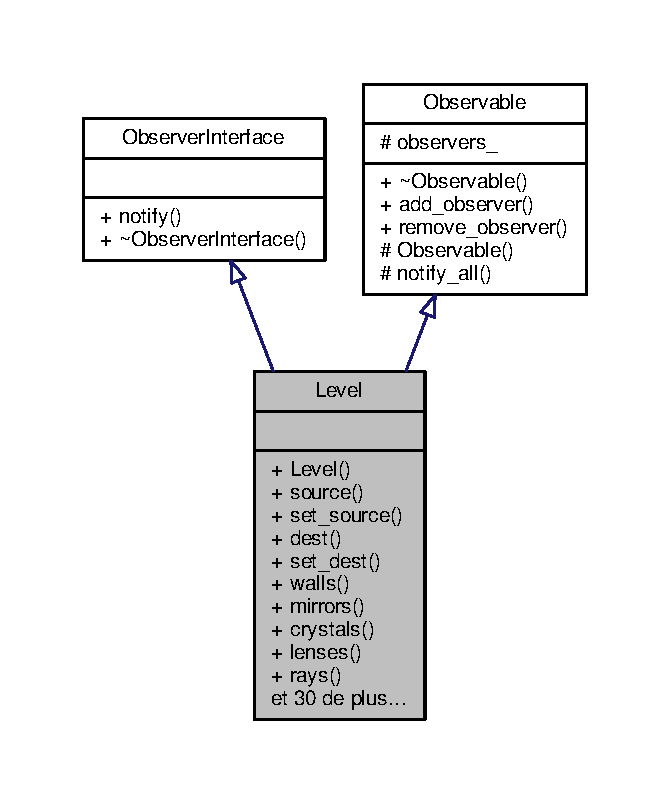
\includegraphics[width=259pt]{dd/d9f/classLevel__inherit__graph}
\end{center}
\end{figure}


Graphe de collaboration de Level\+:
\nopagebreak
\begin{figure}[H]
\begin{center}
\leavevmode
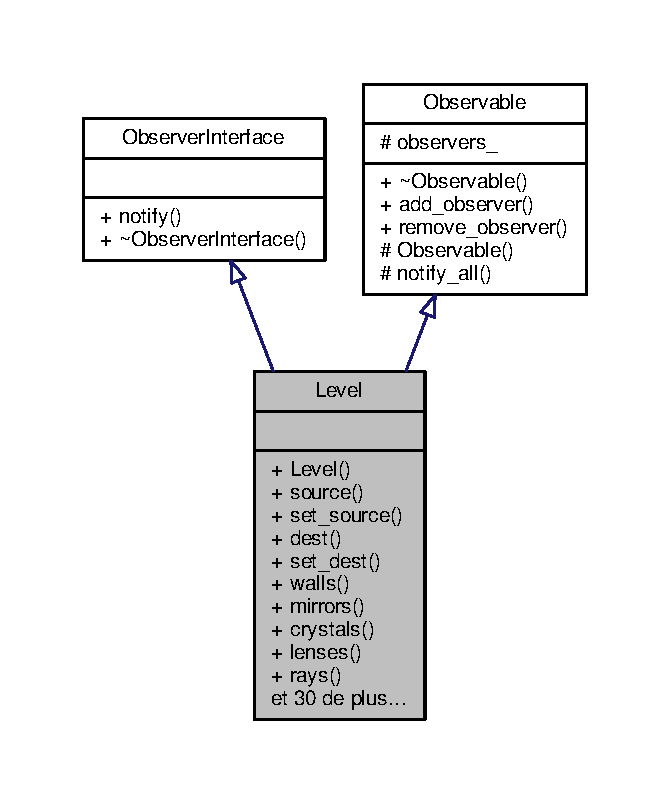
\includegraphics[width=259pt]{df/dee/classLevel__coll__graph}
\end{center}
\end{figure}
\subsection*{Fonctions membres publiques}
\begin{DoxyCompactItemize}
\item 
\hyperlink{classLevel_a36092f5c2dc5d1cace19cbdea946b1a4}{Level} (double w, double h)
\begin{DoxyCompactList}\small\item\em Instancie une carte de largeur et hauteur donnée. \end{DoxyCompactList}\item 
const \hyperlink{classSource}{Source} \& \hyperlink{classLevel_a4f7eb7f4859a1bcc436e51f9e31c64b7}{source} () const 
\begin{DoxyCompactList}\small\item\em Retourne la source de la carte. \end{DoxyCompactList}\item 
void \hyperlink{classLevel_af6c587419e5fac477e4ba530ac9ca327}{set\+\_\+source} (const \hyperlink{classSource}{Source} \&value)
\begin{DoxyCompactList}\small\item\em Change la source de la carte. \end{DoxyCompactList}\item 
const \hyperlink{classDest}{Dest} \& \hyperlink{classLevel_a2d068b34ef9af207645054336e5e19d7}{dest} () const 
\begin{DoxyCompactList}\small\item\em Retourne la desination de la carte. \end{DoxyCompactList}\item 
void \hyperlink{classLevel_a86a9a5ad741890af1501e4ede4022d1a}{set\+\_\+dest} (const \hyperlink{classDest}{Dest} \&value)
\begin{DoxyCompactList}\small\item\em Change la destination de la carte. \end{DoxyCompactList}\item 
const std\+::vector$<$ \hyperlink{classWall}{Wall} $>$ \& \hyperlink{classLevel_add82438c31441eaf067b3c4c290c34bc}{walls} () const 
\begin{DoxyCompactList}\small\item\em Retourne l'ensemble des murs de la carte. \end{DoxyCompactList}\item 
const std\+::vector$<$ \hyperlink{classMirror}{Mirror} $>$ \& \hyperlink{classLevel_aa135dbdea931709337ffcb2fd1ac6b68}{mirrors} () const 
\begin{DoxyCompactList}\small\item\em Retourne l'ensemble des miroirs de la carte. \end{DoxyCompactList}\item 
const std\+::vector$<$ \hyperlink{classCrystal}{Crystal} $>$ \& \hyperlink{classLevel_a5371b5d3d021f9b9cbb3ba4701746ae2}{crystals} () const 
\begin{DoxyCompactList}\small\item\em Retourne l'ensemble des cristaux de la carte. \end{DoxyCompactList}\item 
const std\+::vector$<$ \hyperlink{classLens}{Lens} $>$ \& \hyperlink{classLevel_aca6b1af0d4c00c50922bcc1af73f102b}{lenses} () const 
\begin{DoxyCompactList}\small\item\em Retourne l'ensemble des lentilles de la carte. \end{DoxyCompactList}\item 
const std\+::vector$<$ \hyperlink{classRay}{Ray} $>$ \& \hyperlink{classLevel_acf3ca670d2e2c3c0652dcc66f254cdb6}{rays} () const 
\begin{DoxyCompactList}\small\item\em Retourne l'ensemble des rayons de la carte. \end{DoxyCompactList}\item 
const std\+::vector$<$ \hyperlink{classNuke}{Nuke} $>$ \& \hyperlink{classLevel_acd20c7d517d45796dd33bf9846469cd5}{nukes} () const 
\begin{DoxyCompactList}\small\item\em Retourne l'ensemble des bombes de la carte. \end{DoxyCompactList}\item 
void \hyperlink{classLevel_a55b2185003fbd176c342f4ff014919d0}{set\+\_\+rays} (const std\+::vector$<$ \hyperlink{classRay}{Ray} $>$ \&\hyperlink{classLevel_acf3ca670d2e2c3c0652dcc66f254cdb6}{rays})
\begin{DoxyCompactList}\small\item\em Change l'ensemble des rayons de la carte. \end{DoxyCompactList}\item 
void \hyperlink{classLevel_a35671c58a119ab9c7e6fb4650b8e8fb9}{set\+\_\+walls} (const std\+::vector$<$ \hyperlink{classWall}{Wall} $>$ \&\hyperlink{classLevel_add82438c31441eaf067b3c4c290c34bc}{walls})
\begin{DoxyCompactList}\small\item\em Change l'ensemble des murs de la carte. \end{DoxyCompactList}\item 
void \hyperlink{classLevel_ab1c04c615e4cd6ab36269c8c4a877d06}{set\+\_\+crystals} (const std\+::vector$<$ \hyperlink{classCrystal}{Crystal} $>$ \&\hyperlink{classLevel_a5371b5d3d021f9b9cbb3ba4701746ae2}{crystals})
\begin{DoxyCompactList}\small\item\em Change l'ensemble des cristaux de la carte. \end{DoxyCompactList}\item 
void \hyperlink{classLevel_a83067f34c93b767859ee94c3d1921a42}{set\+\_\+nukes} (const std\+::vector$<$ \hyperlink{classNuke}{Nuke} $>$ \&\hyperlink{classLevel_acd20c7d517d45796dd33bf9846469cd5}{nukes})
\begin{DoxyCompactList}\small\item\em Change l'ensemble des bombes de la carte. \end{DoxyCompactList}\item 
void \hyperlink{classLevel_a94b1dd81fc9d646b5ccd3b52d7702aa4}{set\+\_\+lenses} (const std\+::vector$<$ \hyperlink{classLens}{Lens} $>$ \&\hyperlink{classLevel_aca6b1af0d4c00c50922bcc1af73f102b}{lenses})
\begin{DoxyCompactList}\small\item\em Change l'ensemble des lentilles de la carte. \end{DoxyCompactList}\item 
void \hyperlink{classLevel_a1c18d7c9c016439a995d6d21a03a9470}{set\+\_\+mirrors} (const std\+::vector$<$ \hyperlink{classMirror}{Mirror} $>$ \&\hyperlink{classLevel_aa135dbdea931709337ffcb2fd1ac6b68}{mirrors})
\begin{DoxyCompactList}\small\item\em Change l'ensemble des mirroirs de la carte. \end{DoxyCompactList}\item 
int \hyperlink{classLevel_ac45aad2aa6f8d83f3a619a70f6543ecc}{height} () const 
\begin{DoxyCompactList}\small\item\em Retourne la taille de la carte. \end{DoxyCompactList}\item 
int \hyperlink{classLevel_ad24f669bee981e8d8e688f5d7fad1cc2}{width} () const 
\begin{DoxyCompactList}\small\item\em Retourne la longueur de la carte. \end{DoxyCompactList}\item 
void \hyperlink{classLevel_a731133a250f6ee38179716b3c7492636}{compute\+\_\+rays} ()
\begin{DoxyCompactList}\small\item\em Calcule les rayons lumineux de la carte. \end{DoxyCompactList}\item 
void \hyperlink{classLevel_ac3fe5b4a3cbf3853bbfbd5def8da181b}{add\+\_\+mirror} (const \hyperlink{classMirror}{Mirror} \&m)
\begin{DoxyCompactList}\small\item\em Ajoute un nouveau miroir à la carte. \end{DoxyCompactList}\item 
void \hyperlink{classLevel_a23e8bee1248893bbaeafc551d12982dc}{add\+\_\+nuke} (const \hyperlink{classNuke}{Nuke} \&n)
\begin{DoxyCompactList}\small\item\em Ajoute une nouvelle bombe à la carte. \end{DoxyCompactList}\item 
void \hyperlink{classLevel_a3de8f6b316f8b76aec53ac65ee52e418}{add\+\_\+wall} (const \hyperlink{classWall}{Wall} \&w)
\begin{DoxyCompactList}\small\item\em Ajoute un nouveau mur à la carte. \end{DoxyCompactList}\item 
void \hyperlink{classLevel_a2e9fbec678c73af65ee2500e70241239}{add\+\_\+crystal} (const \hyperlink{classCrystal}{Crystal} \&c)
\begin{DoxyCompactList}\small\item\em Ajoute un nouveau cristal à la carte. \end{DoxyCompactList}\item 
void \hyperlink{classLevel_ac8ace9b9f500c703e376c8f938cad6fe}{add\+\_\+lens} (const \hyperlink{classLens}{Lens} \&l)
\begin{DoxyCompactList}\small\item\em Ajoute une nouvelle lentille à la carte. \end{DoxyCompactList}\item 
void \hyperlink{classLevel_a596a53b1da4d70ce8e0f702e030861cc}{add\+\_\+ray} (const \hyperlink{classRay}{Ray} \&r)
\begin{DoxyCompactList}\small\item\em Ajoute un nouveau rayon à la carte. \end{DoxyCompactList}\item 
bool \hyperlink{classLevel_ad59e370eb6cd2612958208415f90b3ea}{won} () const 
\begin{DoxyCompactList}\small\item\em Retourne vrai si la partie est gagnée. \end{DoxyCompactList}\item 
bool \hyperlink{classLevel_ae6ba86e3567237e12f02f0cd86fc9eeb}{lost} () const 
\begin{DoxyCompactList}\small\item\em Retourne vrai si la partie est perdue. \end{DoxyCompactList}\item 
bool \hyperlink{classLevel_a0271a3a3e893573fa8f1095288def522}{handle\+\_\+nukes} () const 
\begin{DoxyCompactList}\small\item\em Retourne vrai si les nukes sont activées. \end{DoxyCompactList}\item 
bool \hyperlink{classLevel_afcf1375baa8203db70938a45edf701dd}{handle\+\_\+dest} () const 
\begin{DoxyCompactList}\small\item\em Retourne vrai si la destination est activée. \end{DoxyCompactList}\item 
bool \hyperlink{classLevel_a508860af696c5ebd84ec770e3c5d8eac}{check\+\_\+collisions} () const 
\begin{DoxyCompactList}\small\item\em Retourne vrai si les collisions entre les miroirs et les élements de la carte sont gérées. \end{DoxyCompactList}\item 
void \hyperlink{classLevel_a60d687f486e7c2517527b039feeafaae}{set\+\_\+check\+\_\+collisions} (bool value)
\begin{DoxyCompactList}\small\item\em Modifie la vérification des collisions entre miroirs et élements de la carte. \end{DoxyCompactList}\item 
void \hyperlink{classLevel_a27b98ccf50326ca83802de21ab4ea988}{set\+\_\+handle\+\_\+nukes} (bool value)
\begin{DoxyCompactList}\small\item\em Modifie le comportement des nukes de la carte. \end{DoxyCompactList}\item 
void \hyperlink{classLevel_a8334748aff161979d9184fa9dcd93062}{set\+\_\+handle\+\_\+dest} (bool value)
\begin{DoxyCompactList}\small\item\em Modifie le comportement de la destination sur la carte. \end{DoxyCompactList}\item 
void \hyperlink{classLevel_a764f18515935d4b707fd00c8889147fc}{remove\+\_\+crystal} (const \hyperlink{classCrystal}{Crystal} \&c)
\begin{DoxyCompactList}\small\item\em Supprime un crystal. \end{DoxyCompactList}\item 
void \hyperlink{classLevel_acbde0a8bba52e8f7410fc8def32d29e5}{remove\+\_\+lens} (const \hyperlink{classLens}{Lens} \&l)
\begin{DoxyCompactList}\small\item\em Supprime une lentille. \end{DoxyCompactList}\item 
void \hyperlink{classLevel_a32f71b8f1a06fc1be2fec511c47e5aec}{remove\+\_\+mirror} (const \hyperlink{classMirror}{Mirror} \&m)
\begin{DoxyCompactList}\small\item\em Supprime un mirroir. \end{DoxyCompactList}\item 
void \hyperlink{classLevel_ab88f940133cdc4c052ef48b36269e069}{remove\+\_\+nuke} (const \hyperlink{classNuke}{Nuke} \&n)
\begin{DoxyCompactList}\small\item\em Supprime une bombe. \end{DoxyCompactList}\item 
void \hyperlink{classLevel_a0ee86d08a44f0dfca782e7203f830fd1}{remove\+\_\+wall} (const \hyperlink{classWall}{Wall} \&w)
\begin{DoxyCompactList}\small\item\em Supprime un mur. \end{DoxyCompactList}\item 
void \hyperlink{classLevel_adad9e9736501636ce719b5df3725a51f}{notify} (\hyperlink{classObservable}{Observable} $\ast$o, std\+::string msg, const std\+::vector$<$ std\+::string $>$ \&args=std\+::vector$<$ std\+::string $>$())
\begin{DoxyCompactList}\small\item\em Notifie le jeu d'un évènement provenant d'un sujet d'observation (\hyperlink{classObservable}{Observable}). \end{DoxyCompactList}\end{DoxyCompactItemize}
\subsection*{Membres hérités additionnels}


\subsection{Description détaillée}
Modélise une carte telle qu'utilisée dans le jeu. 

Une carte est un ensemble de composants tels que des murs, des miroirs, etc. 

\subsection{Documentation des constructeurs et destructeur}
\hypertarget{classLevel_a36092f5c2dc5d1cace19cbdea946b1a4}{\index{Level@{Level}!Level@{Level}}
\index{Level@{Level}!Level@{Level}}
\subsubsection[{Level}]{\setlength{\rightskip}{0pt plus 5cm}Level\+::\+Level (
\begin{DoxyParamCaption}
\item[{double}]{w, }
\item[{double}]{h}
\end{DoxyParamCaption}
)}}\label{classLevel_a36092f5c2dc5d1cace19cbdea946b1a4}


Instancie une carte de largeur et hauteur donnée. 

Quand une carte est créée, quatre murs dénotant ses bords sont automatiquement ajoutés à la carte. 

La source et la destination sont initialisées à des valeurs par défaut inutilisables. Vous devez manuellement initialiser la source et la destination via les fonctions appropriées. 
\begin{DoxyParams}{Paramètres}
{\em w} & la largeur de la carte. \\
\hline
{\em h} & la hauteur de la carte. \\
\hline
\end{DoxyParams}


\subsection{Documentation des fonctions membres}
\hypertarget{classLevel_a2e9fbec678c73af65ee2500e70241239}{\index{Level@{Level}!add\+\_\+crystal@{add\+\_\+crystal}}
\index{add\+\_\+crystal@{add\+\_\+crystal}!Level@{Level}}
\subsubsection[{add\+\_\+crystal}]{\setlength{\rightskip}{0pt plus 5cm}void Level\+::add\+\_\+crystal (
\begin{DoxyParamCaption}
\item[{const {\bf Crystal} \&}]{c}
\end{DoxyParamCaption}
)\hspace{0.3cm}{\ttfamily [inline]}}}\label{classLevel_a2e9fbec678c73af65ee2500e70241239}


Ajoute un nouveau cristal à la carte. 


\begin{DoxyParams}{Paramètres}
{\em c} & le nouveau cristal. \\
\hline
\end{DoxyParams}
\hypertarget{classLevel_ac8ace9b9f500c703e376c8f938cad6fe}{\index{Level@{Level}!add\+\_\+lens@{add\+\_\+lens}}
\index{add\+\_\+lens@{add\+\_\+lens}!Level@{Level}}
\subsubsection[{add\+\_\+lens}]{\setlength{\rightskip}{0pt plus 5cm}void Level\+::add\+\_\+lens (
\begin{DoxyParamCaption}
\item[{const {\bf Lens} \&}]{l}
\end{DoxyParamCaption}
)\hspace{0.3cm}{\ttfamily [inline]}}}\label{classLevel_ac8ace9b9f500c703e376c8f938cad6fe}


Ajoute une nouvelle lentille à la carte. 


\begin{DoxyParams}{Paramètres}
{\em l} & la nouvelle lentille. \\
\hline
\end{DoxyParams}
\hypertarget{classLevel_ac3fe5b4a3cbf3853bbfbd5def8da181b}{\index{Level@{Level}!add\+\_\+mirror@{add\+\_\+mirror}}
\index{add\+\_\+mirror@{add\+\_\+mirror}!Level@{Level}}
\subsubsection[{add\+\_\+mirror}]{\setlength{\rightskip}{0pt plus 5cm}void Level\+::add\+\_\+mirror (
\begin{DoxyParamCaption}
\item[{const {\bf Mirror} \&}]{m}
\end{DoxyParamCaption}
)\hspace{0.3cm}{\ttfamily [inline]}}}\label{classLevel_ac3fe5b4a3cbf3853bbfbd5def8da181b}


Ajoute un nouveau miroir à la carte. 


\begin{DoxyParams}{Paramètres}
{\em m} & le nouveau miroir. \\
\hline
\end{DoxyParams}
\hypertarget{classLevel_a23e8bee1248893bbaeafc551d12982dc}{\index{Level@{Level}!add\+\_\+nuke@{add\+\_\+nuke}}
\index{add\+\_\+nuke@{add\+\_\+nuke}!Level@{Level}}
\subsubsection[{add\+\_\+nuke}]{\setlength{\rightskip}{0pt plus 5cm}void Level\+::add\+\_\+nuke (
\begin{DoxyParamCaption}
\item[{const {\bf Nuke} \&}]{n}
\end{DoxyParamCaption}
)\hspace{0.3cm}{\ttfamily [inline]}}}\label{classLevel_a23e8bee1248893bbaeafc551d12982dc}


Ajoute une nouvelle bombe à la carte. 


\begin{DoxyParams}{Paramètres}
{\em n} & la nouvelle bombe. \\
\hline
\end{DoxyParams}
\hypertarget{classLevel_a596a53b1da4d70ce8e0f702e030861cc}{\index{Level@{Level}!add\+\_\+ray@{add\+\_\+ray}}
\index{add\+\_\+ray@{add\+\_\+ray}!Level@{Level}}
\subsubsection[{add\+\_\+ray}]{\setlength{\rightskip}{0pt plus 5cm}void Level\+::add\+\_\+ray (
\begin{DoxyParamCaption}
\item[{const {\bf Ray} \&}]{r}
\end{DoxyParamCaption}
)\hspace{0.3cm}{\ttfamily [inline]}}}\label{classLevel_a596a53b1da4d70ce8e0f702e030861cc}


Ajoute un nouveau rayon à la carte. 


\begin{DoxyParams}{Paramètres}
{\em r} & le nouveau rayon. \\
\hline
\end{DoxyParams}
\hypertarget{classLevel_a3de8f6b316f8b76aec53ac65ee52e418}{\index{Level@{Level}!add\+\_\+wall@{add\+\_\+wall}}
\index{add\+\_\+wall@{add\+\_\+wall}!Level@{Level}}
\subsubsection[{add\+\_\+wall}]{\setlength{\rightskip}{0pt plus 5cm}void Level\+::add\+\_\+wall (
\begin{DoxyParamCaption}
\item[{const {\bf Wall} \&}]{w}
\end{DoxyParamCaption}
)\hspace{0.3cm}{\ttfamily [inline]}}}\label{classLevel_a3de8f6b316f8b76aec53ac65ee52e418}


Ajoute un nouveau mur à la carte. 


\begin{DoxyParams}{Paramètres}
{\em w} & le nouveau mur. \\
\hline
\end{DoxyParams}
\hypertarget{classLevel_a508860af696c5ebd84ec770e3c5d8eac}{\index{Level@{Level}!check\+\_\+collisions@{check\+\_\+collisions}}
\index{check\+\_\+collisions@{check\+\_\+collisions}!Level@{Level}}
\subsubsection[{check\+\_\+collisions}]{\setlength{\rightskip}{0pt plus 5cm}bool Level\+::check\+\_\+collisions (
\begin{DoxyParamCaption}
{}
\end{DoxyParamCaption}
) const\hspace{0.3cm}{\ttfamily [inline]}}}\label{classLevel_a508860af696c5ebd84ec770e3c5d8eac}


Retourne vrai si les collisions entre les miroirs et les élements de la carte sont gérées. 

\begin{DoxyReturn}{Renvoie}
vrai si les collisions sont gérées, faux sinon. 
\end{DoxyReturn}
\hypertarget{classLevel_a731133a250f6ee38179716b3c7492636}{\index{Level@{Level}!compute\+\_\+rays@{compute\+\_\+rays}}
\index{compute\+\_\+rays@{compute\+\_\+rays}!Level@{Level}}
\subsubsection[{compute\+\_\+rays}]{\setlength{\rightskip}{0pt plus 5cm}void Level\+::compute\+\_\+rays (
\begin{DoxyParamCaption}
{}
\end{DoxyParamCaption}
)}}\label{classLevel_a731133a250f6ee38179716b3c7492636}


Calcule les rayons lumineux de la carte. 

Cette fonction doit être surchargée obligatoirement. \hypertarget{classLevel_a5371b5d3d021f9b9cbb3ba4701746ae2}{\index{Level@{Level}!crystals@{crystals}}
\index{crystals@{crystals}!Level@{Level}}
\subsubsection[{crystals}]{\setlength{\rightskip}{0pt plus 5cm}const std\+::vector$<$ {\bf Crystal} $>$ \& Level\+::crystals (
\begin{DoxyParamCaption}
{}
\end{DoxyParamCaption}
) const\hspace{0.3cm}{\ttfamily [inline]}}}\label{classLevel_a5371b5d3d021f9b9cbb3ba4701746ae2}


Retourne l'ensemble des cristaux de la carte. 

\begin{DoxyReturn}{Renvoie}
l'ensemble des cristaux de la carte. 
\end{DoxyReturn}
\hypertarget{classLevel_a2d068b34ef9af207645054336e5e19d7}{\index{Level@{Level}!dest@{dest}}
\index{dest@{dest}!Level@{Level}}
\subsubsection[{dest}]{\setlength{\rightskip}{0pt plus 5cm}const {\bf Dest} \& Level\+::dest (
\begin{DoxyParamCaption}
{}
\end{DoxyParamCaption}
) const\hspace{0.3cm}{\ttfamily [inline]}}}\label{classLevel_a2d068b34ef9af207645054336e5e19d7}


Retourne la desination de la carte. 

\begin{DoxyReturn}{Renvoie}
la destination de la carte. 
\end{DoxyReturn}
\hypertarget{classLevel_afcf1375baa8203db70938a45edf701dd}{\index{Level@{Level}!handle\+\_\+dest@{handle\+\_\+dest}}
\index{handle\+\_\+dest@{handle\+\_\+dest}!Level@{Level}}
\subsubsection[{handle\+\_\+dest}]{\setlength{\rightskip}{0pt plus 5cm}bool Level\+::handle\+\_\+dest (
\begin{DoxyParamCaption}
{}
\end{DoxyParamCaption}
) const\hspace{0.3cm}{\ttfamily [inline]}}}\label{classLevel_afcf1375baa8203db70938a45edf701dd}


Retourne vrai si la destination est activée. 

\begin{DoxyReturn}{Renvoie}
vrai si la destination est activée, faux sinon. 
\end{DoxyReturn}
\hypertarget{classLevel_a0271a3a3e893573fa8f1095288def522}{\index{Level@{Level}!handle\+\_\+nukes@{handle\+\_\+nukes}}
\index{handle\+\_\+nukes@{handle\+\_\+nukes}!Level@{Level}}
\subsubsection[{handle\+\_\+nukes}]{\setlength{\rightskip}{0pt plus 5cm}bool Level\+::handle\+\_\+nukes (
\begin{DoxyParamCaption}
{}
\end{DoxyParamCaption}
) const\hspace{0.3cm}{\ttfamily [inline]}}}\label{classLevel_a0271a3a3e893573fa8f1095288def522}


Retourne vrai si les nukes sont activées. 

\begin{DoxyReturn}{Renvoie}
vrai si les nukes sont activées, faux sinon. 
\end{DoxyReturn}
\hypertarget{classLevel_ac45aad2aa6f8d83f3a619a70f6543ecc}{\index{Level@{Level}!height@{height}}
\index{height@{height}!Level@{Level}}
\subsubsection[{height}]{\setlength{\rightskip}{0pt plus 5cm}int Level\+::height (
\begin{DoxyParamCaption}
{}
\end{DoxyParamCaption}
) const\hspace{0.3cm}{\ttfamily [inline]}}}\label{classLevel_ac45aad2aa6f8d83f3a619a70f6543ecc}


Retourne la taille de la carte. 

\begin{DoxyReturn}{Renvoie}
la taille de la carte. 
\end{DoxyReturn}
\hypertarget{classLevel_aca6b1af0d4c00c50922bcc1af73f102b}{\index{Level@{Level}!lenses@{lenses}}
\index{lenses@{lenses}!Level@{Level}}
\subsubsection[{lenses}]{\setlength{\rightskip}{0pt plus 5cm}const std\+::vector$<$ {\bf Lens} $>$ \& Level\+::lenses (
\begin{DoxyParamCaption}
{}
\end{DoxyParamCaption}
) const\hspace{0.3cm}{\ttfamily [inline]}}}\label{classLevel_aca6b1af0d4c00c50922bcc1af73f102b}


Retourne l'ensemble des lentilles de la carte. 

\begin{DoxyReturn}{Renvoie}
l'ensemble des lentilles de la carte. 
\end{DoxyReturn}
\hypertarget{classLevel_ae6ba86e3567237e12f02f0cd86fc9eeb}{\index{Level@{Level}!lost@{lost}}
\index{lost@{lost}!Level@{Level}}
\subsubsection[{lost}]{\setlength{\rightskip}{0pt plus 5cm}bool Level\+::lost (
\begin{DoxyParamCaption}
{}
\end{DoxyParamCaption}
) const\hspace{0.3cm}{\ttfamily [inline]}}}\label{classLevel_ae6ba86e3567237e12f02f0cd86fc9eeb}


Retourne vrai si la partie est perdue. 

\begin{DoxyReturn}{Renvoie}
vrai si la partie est perdue, faux sinon. 
\end{DoxyReturn}
\hypertarget{classLevel_aa135dbdea931709337ffcb2fd1ac6b68}{\index{Level@{Level}!mirrors@{mirrors}}
\index{mirrors@{mirrors}!Level@{Level}}
\subsubsection[{mirrors}]{\setlength{\rightskip}{0pt plus 5cm}const std\+::vector$<$ {\bf Mirror} $>$ \& Level\+::mirrors (
\begin{DoxyParamCaption}
{}
\end{DoxyParamCaption}
) const\hspace{0.3cm}{\ttfamily [inline]}}}\label{classLevel_aa135dbdea931709337ffcb2fd1ac6b68}


Retourne l'ensemble des miroirs de la carte. 

\begin{DoxyReturn}{Renvoie}
l'ensemble des miroirs de la carte. 
\end{DoxyReturn}
\hypertarget{classLevel_adad9e9736501636ce719b5df3725a51f}{\index{Level@{Level}!notify@{notify}}
\index{notify@{notify}!Level@{Level}}
\subsubsection[{notify}]{\setlength{\rightskip}{0pt plus 5cm}void Level\+::notify (
\begin{DoxyParamCaption}
\item[{{\bf Observable} $\ast$}]{sdo, }
\item[{std\+::string}]{msg, }
\item[{const std\+::vector$<$ std\+::string $>$ \&}]{args = {\ttfamily std\+:\+:vector$<$~std\+:\+:string~$>$()}}
\end{DoxyParamCaption}
)\hspace{0.3cm}{\ttfamily [virtual]}}}\label{classLevel_adad9e9736501636ce719b5df3725a51f}


Notifie le jeu d'un évènement provenant d'un sujet d'observation (\hyperlink{classObservable}{Observable}). 


\begin{DoxyParams}{Paramètres}
{\em o} & l'observé. \\
\hline
{\em msg} & le message de notification. \\
\hline
{\em args} & des arguments. \\
\hline
\end{DoxyParams}


Implémente \hyperlink{classObserverInterface_a1bbd22519c2942d978804714db12c8b2}{Observer\+Interface}.

\hypertarget{classLevel_acd20c7d517d45796dd33bf9846469cd5}{\index{Level@{Level}!nukes@{nukes}}
\index{nukes@{nukes}!Level@{Level}}
\subsubsection[{nukes}]{\setlength{\rightskip}{0pt plus 5cm}const std\+::vector$<$ {\bf Nuke} $>$ \& Level\+::nukes (
\begin{DoxyParamCaption}
{}
\end{DoxyParamCaption}
) const\hspace{0.3cm}{\ttfamily [inline]}}}\label{classLevel_acd20c7d517d45796dd33bf9846469cd5}


Retourne l'ensemble des bombes de la carte. 

\begin{DoxyReturn}{Renvoie}
l'ensemble des bombes de la carte. 
\end{DoxyReturn}
\hypertarget{classLevel_acf3ca670d2e2c3c0652dcc66f254cdb6}{\index{Level@{Level}!rays@{rays}}
\index{rays@{rays}!Level@{Level}}
\subsubsection[{rays}]{\setlength{\rightskip}{0pt plus 5cm}const std\+::vector$<$ {\bf Ray} $>$ \& Level\+::rays (
\begin{DoxyParamCaption}
{}
\end{DoxyParamCaption}
) const\hspace{0.3cm}{\ttfamily [inline]}}}\label{classLevel_acf3ca670d2e2c3c0652dcc66f254cdb6}


Retourne l'ensemble des rayons de la carte. 

\begin{DoxyReturn}{Renvoie}
l'ensemble des rayons de la carte. 
\end{DoxyReturn}
\hypertarget{classLevel_a764f18515935d4b707fd00c8889147fc}{\index{Level@{Level}!remove\+\_\+crystal@{remove\+\_\+crystal}}
\index{remove\+\_\+crystal@{remove\+\_\+crystal}!Level@{Level}}
\subsubsection[{remove\+\_\+crystal}]{\setlength{\rightskip}{0pt plus 5cm}void Level\+::remove\+\_\+crystal (
\begin{DoxyParamCaption}
\item[{const {\bf Crystal} \&}]{c}
\end{DoxyParamCaption}
)\hspace{0.3cm}{\ttfamily [inline]}}}\label{classLevel_a764f18515935d4b707fd00c8889147fc}


Supprime un crystal. 


\begin{DoxyParams}{Paramètres}
{\em c} & le crystal à supprimer. \\
\hline
\end{DoxyParams}
\hypertarget{classLevel_acbde0a8bba52e8f7410fc8def32d29e5}{\index{Level@{Level}!remove\+\_\+lens@{remove\+\_\+lens}}
\index{remove\+\_\+lens@{remove\+\_\+lens}!Level@{Level}}
\subsubsection[{remove\+\_\+lens}]{\setlength{\rightskip}{0pt plus 5cm}void Level\+::remove\+\_\+lens (
\begin{DoxyParamCaption}
\item[{const {\bf Lens} \&}]{l}
\end{DoxyParamCaption}
)\hspace{0.3cm}{\ttfamily [inline]}}}\label{classLevel_acbde0a8bba52e8f7410fc8def32d29e5}


Supprime une lentille. 


\begin{DoxyParams}{Paramètres}
{\em l} & la lentille à supprimer. \\
\hline
\end{DoxyParams}
\hypertarget{classLevel_a32f71b8f1a06fc1be2fec511c47e5aec}{\index{Level@{Level}!remove\+\_\+mirror@{remove\+\_\+mirror}}
\index{remove\+\_\+mirror@{remove\+\_\+mirror}!Level@{Level}}
\subsubsection[{remove\+\_\+mirror}]{\setlength{\rightskip}{0pt plus 5cm}void Level\+::remove\+\_\+mirror (
\begin{DoxyParamCaption}
\item[{const {\bf Mirror} \&}]{m}
\end{DoxyParamCaption}
)\hspace{0.3cm}{\ttfamily [inline]}}}\label{classLevel_a32f71b8f1a06fc1be2fec511c47e5aec}


Supprime un mirroir. 


\begin{DoxyParams}{Paramètres}
{\em m} & le mirroir à supprimer. \\
\hline
\end{DoxyParams}
\hypertarget{classLevel_ab88f940133cdc4c052ef48b36269e069}{\index{Level@{Level}!remove\+\_\+nuke@{remove\+\_\+nuke}}
\index{remove\+\_\+nuke@{remove\+\_\+nuke}!Level@{Level}}
\subsubsection[{remove\+\_\+nuke}]{\setlength{\rightskip}{0pt plus 5cm}void Level\+::remove\+\_\+nuke (
\begin{DoxyParamCaption}
\item[{const {\bf Nuke} \&}]{n}
\end{DoxyParamCaption}
)\hspace{0.3cm}{\ttfamily [inline]}}}\label{classLevel_ab88f940133cdc4c052ef48b36269e069}


Supprime une bombe. 


\begin{DoxyParams}{Paramètres}
{\em n} & la bombe à supprimer. \\
\hline
\end{DoxyParams}
\hypertarget{classLevel_a0ee86d08a44f0dfca782e7203f830fd1}{\index{Level@{Level}!remove\+\_\+wall@{remove\+\_\+wall}}
\index{remove\+\_\+wall@{remove\+\_\+wall}!Level@{Level}}
\subsubsection[{remove\+\_\+wall}]{\setlength{\rightskip}{0pt plus 5cm}void Level\+::remove\+\_\+wall (
\begin{DoxyParamCaption}
\item[{const {\bf Wall} \&}]{w}
\end{DoxyParamCaption}
)\hspace{0.3cm}{\ttfamily [inline]}}}\label{classLevel_a0ee86d08a44f0dfca782e7203f830fd1}


Supprime un mur. 


\begin{DoxyParams}{Paramètres}
{\em w} & le mur à supprimer. \\
\hline
\end{DoxyParams}
\hypertarget{classLevel_a60d687f486e7c2517527b039feeafaae}{\index{Level@{Level}!set\+\_\+check\+\_\+collisions@{set\+\_\+check\+\_\+collisions}}
\index{set\+\_\+check\+\_\+collisions@{set\+\_\+check\+\_\+collisions}!Level@{Level}}
\subsubsection[{set\+\_\+check\+\_\+collisions}]{\setlength{\rightskip}{0pt plus 5cm}void Level\+::set\+\_\+check\+\_\+collisions (
\begin{DoxyParamCaption}
\item[{bool}]{value}
\end{DoxyParamCaption}
)\hspace{0.3cm}{\ttfamily [inline]}}}\label{classLevel_a60d687f486e7c2517527b039feeafaae}


Modifie la vérification des collisions entre miroirs et élements de la carte. 


\begin{DoxyParams}{Paramètres}
{\em value} & vrai si les collisions sont gérées, faux sinon. \\
\hline
\end{DoxyParams}
\hypertarget{classLevel_ab1c04c615e4cd6ab36269c8c4a877d06}{\index{Level@{Level}!set\+\_\+crystals@{set\+\_\+crystals}}
\index{set\+\_\+crystals@{set\+\_\+crystals}!Level@{Level}}
\subsubsection[{set\+\_\+crystals}]{\setlength{\rightskip}{0pt plus 5cm}void Level\+::set\+\_\+crystals (
\begin{DoxyParamCaption}
\item[{const std\+::vector$<$ {\bf Crystal} $>$ \&}]{crystals}
\end{DoxyParamCaption}
)\hspace{0.3cm}{\ttfamily [inline]}}}\label{classLevel_ab1c04c615e4cd6ab36269c8c4a877d06}


Change l'ensemble des cristaux de la carte. 


\begin{DoxyParams}{Paramètres}
{\em crystals} & le nouvel ensemble des cristaux de la carte. \\
\hline
\end{DoxyParams}
\hypertarget{classLevel_a86a9a5ad741890af1501e4ede4022d1a}{\index{Level@{Level}!set\+\_\+dest@{set\+\_\+dest}}
\index{set\+\_\+dest@{set\+\_\+dest}!Level@{Level}}
\subsubsection[{set\+\_\+dest}]{\setlength{\rightskip}{0pt plus 5cm}void Level\+::set\+\_\+dest (
\begin{DoxyParamCaption}
\item[{const {\bf Dest} \&}]{value}
\end{DoxyParamCaption}
)\hspace{0.3cm}{\ttfamily [inline]}}}\label{classLevel_a86a9a5ad741890af1501e4ede4022d1a}


Change la destination de la carte. 


\begin{DoxyParams}{Paramètres}
{\em value} & la destination de la carte. \\
\hline
\end{DoxyParams}
\hypertarget{classLevel_a8334748aff161979d9184fa9dcd93062}{\index{Level@{Level}!set\+\_\+handle\+\_\+dest@{set\+\_\+handle\+\_\+dest}}
\index{set\+\_\+handle\+\_\+dest@{set\+\_\+handle\+\_\+dest}!Level@{Level}}
\subsubsection[{set\+\_\+handle\+\_\+dest}]{\setlength{\rightskip}{0pt plus 5cm}void Level\+::set\+\_\+handle\+\_\+dest (
\begin{DoxyParamCaption}
\item[{bool}]{value}
\end{DoxyParamCaption}
)\hspace{0.3cm}{\ttfamily [inline]}}}\label{classLevel_a8334748aff161979d9184fa9dcd93062}


Modifie le comportement de la destination sur la carte. 


\begin{DoxyParams}{Paramètres}
{\em value} & vrai si la destination est activée, faux sinon. \\
\hline
\end{DoxyParams}
\hypertarget{classLevel_a27b98ccf50326ca83802de21ab4ea988}{\index{Level@{Level}!set\+\_\+handle\+\_\+nukes@{set\+\_\+handle\+\_\+nukes}}
\index{set\+\_\+handle\+\_\+nukes@{set\+\_\+handle\+\_\+nukes}!Level@{Level}}
\subsubsection[{set\+\_\+handle\+\_\+nukes}]{\setlength{\rightskip}{0pt plus 5cm}void Level\+::set\+\_\+handle\+\_\+nukes (
\begin{DoxyParamCaption}
\item[{bool}]{value}
\end{DoxyParamCaption}
)\hspace{0.3cm}{\ttfamily [inline]}}}\label{classLevel_a27b98ccf50326ca83802de21ab4ea988}


Modifie le comportement des nukes de la carte. 


\begin{DoxyParams}{Paramètres}
{\em value} & vrai si les nukes sont activées, faux sinon. \\
\hline
\end{DoxyParams}
\hypertarget{classLevel_a94b1dd81fc9d646b5ccd3b52d7702aa4}{\index{Level@{Level}!set\+\_\+lenses@{set\+\_\+lenses}}
\index{set\+\_\+lenses@{set\+\_\+lenses}!Level@{Level}}
\subsubsection[{set\+\_\+lenses}]{\setlength{\rightskip}{0pt plus 5cm}void Level\+::set\+\_\+lenses (
\begin{DoxyParamCaption}
\item[{const std\+::vector$<$ {\bf Lens} $>$ \&}]{lenses}
\end{DoxyParamCaption}
)\hspace{0.3cm}{\ttfamily [inline]}}}\label{classLevel_a94b1dd81fc9d646b5ccd3b52d7702aa4}


Change l'ensemble des lentilles de la carte. 


\begin{DoxyParams}{Paramètres}
{\em lenses} & le nouvel ensemble des lentilles de la carte. \\
\hline
\end{DoxyParams}
\hypertarget{classLevel_a1c18d7c9c016439a995d6d21a03a9470}{\index{Level@{Level}!set\+\_\+mirrors@{set\+\_\+mirrors}}
\index{set\+\_\+mirrors@{set\+\_\+mirrors}!Level@{Level}}
\subsubsection[{set\+\_\+mirrors}]{\setlength{\rightskip}{0pt plus 5cm}void Level\+::set\+\_\+mirrors (
\begin{DoxyParamCaption}
\item[{const std\+::vector$<$ {\bf Mirror} $>$ \&}]{mirrors}
\end{DoxyParamCaption}
)\hspace{0.3cm}{\ttfamily [inline]}}}\label{classLevel_a1c18d7c9c016439a995d6d21a03a9470}


Change l'ensemble des mirroirs de la carte. 


\begin{DoxyParams}{Paramètres}
{\em mirrors} & le nouvel ensemble des mirroirs de la carte. \\
\hline
\end{DoxyParams}
\hypertarget{classLevel_a83067f34c93b767859ee94c3d1921a42}{\index{Level@{Level}!set\+\_\+nukes@{set\+\_\+nukes}}
\index{set\+\_\+nukes@{set\+\_\+nukes}!Level@{Level}}
\subsubsection[{set\+\_\+nukes}]{\setlength{\rightskip}{0pt plus 5cm}void Level\+::set\+\_\+nukes (
\begin{DoxyParamCaption}
\item[{const std\+::vector$<$ {\bf Nuke} $>$ \&}]{nukes}
\end{DoxyParamCaption}
)\hspace{0.3cm}{\ttfamily [inline]}}}\label{classLevel_a83067f34c93b767859ee94c3d1921a42}


Change l'ensemble des bombes de la carte. 


\begin{DoxyParams}{Paramètres}
{\em nukes} & le nouvel ensemble des bombes de la carte. \\
\hline
\end{DoxyParams}
\hypertarget{classLevel_a55b2185003fbd176c342f4ff014919d0}{\index{Level@{Level}!set\+\_\+rays@{set\+\_\+rays}}
\index{set\+\_\+rays@{set\+\_\+rays}!Level@{Level}}
\subsubsection[{set\+\_\+rays}]{\setlength{\rightskip}{0pt plus 5cm}void Level\+::set\+\_\+rays (
\begin{DoxyParamCaption}
\item[{const std\+::vector$<$ {\bf Ray} $>$ \&}]{rays}
\end{DoxyParamCaption}
)\hspace{0.3cm}{\ttfamily [inline]}}}\label{classLevel_a55b2185003fbd176c342f4ff014919d0}


Change l'ensemble des rayons de la carte. 


\begin{DoxyParams}{Paramètres}
{\em rays} & le nouvel ensemble de rayons de la carte. \\
\hline
\end{DoxyParams}
\hypertarget{classLevel_af6c587419e5fac477e4ba530ac9ca327}{\index{Level@{Level}!set\+\_\+source@{set\+\_\+source}}
\index{set\+\_\+source@{set\+\_\+source}!Level@{Level}}
\subsubsection[{set\+\_\+source}]{\setlength{\rightskip}{0pt plus 5cm}void Level\+::set\+\_\+source (
\begin{DoxyParamCaption}
\item[{const {\bf Source} \&}]{value}
\end{DoxyParamCaption}
)\hspace{0.3cm}{\ttfamily [inline]}}}\label{classLevel_af6c587419e5fac477e4ba530ac9ca327}


Change la source de la carte. 


\begin{DoxyParams}{Paramètres}
{\em value} & la nouvelle source. \\
\hline
\end{DoxyParams}
\hypertarget{classLevel_a35671c58a119ab9c7e6fb4650b8e8fb9}{\index{Level@{Level}!set\+\_\+walls@{set\+\_\+walls}}
\index{set\+\_\+walls@{set\+\_\+walls}!Level@{Level}}
\subsubsection[{set\+\_\+walls}]{\setlength{\rightskip}{0pt plus 5cm}void Level\+::set\+\_\+walls (
\begin{DoxyParamCaption}
\item[{const std\+::vector$<$ {\bf Wall} $>$ \&}]{walls}
\end{DoxyParamCaption}
)\hspace{0.3cm}{\ttfamily [inline]}}}\label{classLevel_a35671c58a119ab9c7e6fb4650b8e8fb9}


Change l'ensemble des murs de la carte. 


\begin{DoxyParams}{Paramètres}
{\em walls} & le nouvel ensemble de murs de la carte. \\
\hline
\end{DoxyParams}
\hypertarget{classLevel_a4f7eb7f4859a1bcc436e51f9e31c64b7}{\index{Level@{Level}!source@{source}}
\index{source@{source}!Level@{Level}}
\subsubsection[{source}]{\setlength{\rightskip}{0pt plus 5cm}const {\bf Source} \& Level\+::source (
\begin{DoxyParamCaption}
{}
\end{DoxyParamCaption}
) const\hspace{0.3cm}{\ttfamily [inline]}}}\label{classLevel_a4f7eb7f4859a1bcc436e51f9e31c64b7}


Retourne la source de la carte. 

\begin{DoxyReturn}{Renvoie}
la source de la carte. 
\end{DoxyReturn}
\hypertarget{classLevel_add82438c31441eaf067b3c4c290c34bc}{\index{Level@{Level}!walls@{walls}}
\index{walls@{walls}!Level@{Level}}
\subsubsection[{walls}]{\setlength{\rightskip}{0pt plus 5cm}const std\+::vector$<$ {\bf Wall} $>$ \& Level\+::walls (
\begin{DoxyParamCaption}
{}
\end{DoxyParamCaption}
) const\hspace{0.3cm}{\ttfamily [inline]}}}\label{classLevel_add82438c31441eaf067b3c4c290c34bc}


Retourne l'ensemble des murs de la carte. 

\begin{DoxyReturn}{Renvoie}
l'ensemble des murs de la carte. 
\end{DoxyReturn}
\hypertarget{classLevel_ad24f669bee981e8d8e688f5d7fad1cc2}{\index{Level@{Level}!width@{width}}
\index{width@{width}!Level@{Level}}
\subsubsection[{width}]{\setlength{\rightskip}{0pt plus 5cm}int Level\+::width (
\begin{DoxyParamCaption}
{}
\end{DoxyParamCaption}
) const\hspace{0.3cm}{\ttfamily [inline]}}}\label{classLevel_ad24f669bee981e8d8e688f5d7fad1cc2}


Retourne la longueur de la carte. 

\begin{DoxyReturn}{Renvoie}
la longueur de la carte. 
\end{DoxyReturn}
\hypertarget{classLevel_ad59e370eb6cd2612958208415f90b3ea}{\index{Level@{Level}!won@{won}}
\index{won@{won}!Level@{Level}}
\subsubsection[{won}]{\setlength{\rightskip}{0pt plus 5cm}bool Level\+::won (
\begin{DoxyParamCaption}
{}
\end{DoxyParamCaption}
) const\hspace{0.3cm}{\ttfamily [inline]}}}\label{classLevel_ad59e370eb6cd2612958208415f90b3ea}


Retourne vrai si la partie est gagnée. 

\begin{DoxyReturn}{Renvoie}
vrai si la partie est gagnée, faux sinon. 
\end{DoxyReturn}


La documentation de cette classe a été générée à partir des fichiers suivants \+:\begin{DoxyCompactItemize}
\item 
model/level.\+h\item 
model/level.\+cpp\end{DoxyCompactItemize}

\hypertarget{classLine}{\section{Référence de la classe Line}
\label{classLine}\index{Line@{Line}}
}


Cette classe représente une droite sous la forme ax + by + c = 0.  




{\ttfamily \#include $<$line.\+h$>$}

\subsection*{Fonctions membres publiques}
\begin{DoxyCompactItemize}
\item 
\hyperlink{classLine_aba5e77c92e5e6932e90d0c083e6509e5}{Line} (double \hyperlink{classLine_a47fbf6abd88d639659beb7a5c7a22a86}{a}, double \hyperlink{classLine_a3fbf3dbd1b40db13b2624d69ab5cca27}{b}, double \hyperlink{classLine_a178f0e9f733556ef03ba94e5aac96005}{c})
\begin{DoxyCompactList}\small\item\em Instancie une nouvelle droite avec les trois paramètres a, b et c donnés. \end{DoxyCompactList}\item 
\hyperlink{classLine_a0ec34f80a43014768ec228bfa87fd15f}{Line} (const \hyperlink{classPoint}{Point} \&\hyperlink{classLine_a47fbf6abd88d639659beb7a5c7a22a86}{a}, const \hyperlink{classPoint}{Point} \&\hyperlink{classLine_a3fbf3dbd1b40db13b2624d69ab5cca27}{b})
\begin{DoxyCompactList}\small\item\em Instancie une nouvelle droite avec deux points donnés. \end{DoxyCompactList}\item 
\hyperlink{classLine_a30f99e975efe2a498c2d8ad7c9d1cdf2}{Line} (const \hyperlink{classPoint}{Point} \&p, double \hyperlink{classLine_afe0a0abb45c0adccaedfaded8645600f}{alpha})
\begin{DoxyCompactList}\small\item\em Instancie une nouvelle droite avec un point donné et un angle donné. \end{DoxyCompactList}\item 
double \hyperlink{classLine_a47fbf6abd88d639659beb7a5c7a22a86}{a} () const 
\begin{DoxyCompactList}\small\item\em Retourne a. \end{DoxyCompactList}\item 
double \hyperlink{classLine_a3fbf3dbd1b40db13b2624d69ab5cca27}{b} () const 
\begin{DoxyCompactList}\small\item\em Retourne b. \end{DoxyCompactList}\item 
double \hyperlink{classLine_a178f0e9f733556ef03ba94e5aac96005}{c} () const 
\begin{DoxyCompactList}\small\item\em Retourne c. \end{DoxyCompactList}\item 
double \hyperlink{classLine_afe0a0abb45c0adccaedfaded8645600f}{alpha} () const 
\begin{DoxyCompactList}\small\item\em Retourne l'angle produit par la pente de la droite. \end{DoxyCompactList}\item 
double \hyperlink{classLine_a582597e85fc78ba06ccdddf6c270ed71}{slope} () const 
\begin{DoxyCompactList}\small\item\em Retourne la pente de la droite. \end{DoxyCompactList}\item 
double \hyperlink{classLine_a786bca726aa14177ebedbfeddc4bb8e5}{inde\+\_\+param} () const 
\begin{DoxyCompactList}\small\item\em Retourne l'ordonnée à l'origine. \end{DoxyCompactList}\item 
double \hyperlink{classLine_a53605544b400dda2164802a374f25b92}{get\+\_\+x} (const double y) const 
\begin{DoxyCompactList}\small\item\em Retourne le x d'un y donné. \end{DoxyCompactList}\item 
double \hyperlink{classLine_abe48fc1d77385ea5a80dc0a314127cff}{get\+\_\+y} (const double x) const 
\begin{DoxyCompactList}\small\item\em Retourne le y d'un x donné. \end{DoxyCompactList}\item 
bool \hyperlink{classLine_a8774606646298fb27a6e158af5e84590}{vertical} () const 
\begin{DoxyCompactList}\small\item\em Retourne vrai si la droite est verticale. \end{DoxyCompactList}\item 
bool \hyperlink{classLine_a1be7d198aeee493e6fba56f09057b4a6}{horizontal} () const 
\begin{DoxyCompactList}\small\item\em Retourne vrai si la droite est horizontale. \end{DoxyCompactList}\item 
bool \hyperlink{classLine_a3655584ad1c2958e4ab9c3ee9a3e6eed}{parallel} (const \hyperlink{classLine}{Line} \&l) const 
\begin{DoxyCompactList}\small\item\em Retourne vrai si une droite est parallèle ou confondu à la droite. \end{DoxyCompactList}\item 
bool \hyperlink{classLine_a208642b69677aba26b05bf6f29ebff19}{perpendicular} (const \hyperlink{classLine}{Line} \&l) const 
\begin{DoxyCompactList}\small\item\em Retourne vrai si une droite est perpendiculaire à la droite. \end{DoxyCompactList}\item 
bool \hyperlink{classLine_a80ee8a6411242e1c29d57c4f5adf4bfb}{operator==} (const \hyperlink{classLine}{Line} \&l) const 
\begin{DoxyCompactList}\small\item\em Redéfinition de l'opérateur d'égalité. \end{DoxyCompactList}\end{DoxyCompactItemize}


\subsection{Description détaillée}
Cette classe représente une droite sous la forme ax + by + c = 0. 

Elle possède également un attribut alpha\+\_\+ pour préciser l'angle réel de la droite. Si on veut travailler avec des angles négatifs par exemple. 

\subsection{Documentation des constructeurs et destructeur}
\hypertarget{classLine_aba5e77c92e5e6932e90d0c083e6509e5}{\index{Line@{Line}!Line@{Line}}
\index{Line@{Line}!Line@{Line}}
\subsubsection[{Line}]{\setlength{\rightskip}{0pt plus 5cm}Line\+::\+Line (
\begin{DoxyParamCaption}
\item[{double}]{a, }
\item[{double}]{b, }
\item[{double}]{c}
\end{DoxyParamCaption}
)}}\label{classLine_aba5e77c92e5e6932e90d0c083e6509e5}


Instancie une nouvelle droite avec les trois paramètres a, b et c donnés. 


\begin{DoxyParams}{Paramètres}
{\em a} & a \\
\hline
{\em b} & b \\
\hline
{\em c} & c \\
\hline
\end{DoxyParams}
\hypertarget{classLine_a0ec34f80a43014768ec228bfa87fd15f}{\index{Line@{Line}!Line@{Line}}
\index{Line@{Line}!Line@{Line}}
\subsubsection[{Line}]{\setlength{\rightskip}{0pt plus 5cm}Line\+::\+Line (
\begin{DoxyParamCaption}
\item[{const {\bf Point} \&}]{a, }
\item[{const {\bf Point} \&}]{b}
\end{DoxyParamCaption}
)}}\label{classLine_a0ec34f80a43014768ec228bfa87fd15f}


Instancie une nouvelle droite avec deux points donnés. 


\begin{DoxyParams}{Paramètres}
{\em a} & le premier point. \\
\hline
{\em b} & le deuxième point. \\
\hline
\end{DoxyParams}
\hypertarget{classLine_a30f99e975efe2a498c2d8ad7c9d1cdf2}{\index{Line@{Line}!Line@{Line}}
\index{Line@{Line}!Line@{Line}}
\subsubsection[{Line}]{\setlength{\rightskip}{0pt plus 5cm}Line\+::\+Line (
\begin{DoxyParamCaption}
\item[{const {\bf Point} \&}]{p, }
\item[{double}]{alpha}
\end{DoxyParamCaption}
)}}\label{classLine_a30f99e975efe2a498c2d8ad7c9d1cdf2}


Instancie une nouvelle droite avec un point donné et un angle donné. 


\begin{DoxyParams}{Paramètres}
{\em p} & le point de la droite \\
\hline
{\em alpha} & l'angle de la droite \\
\hline
\end{DoxyParams}


\subsection{Documentation des fonctions membres}
\hypertarget{classLine_a47fbf6abd88d639659beb7a5c7a22a86}{\index{Line@{Line}!a@{a}}
\index{a@{a}!Line@{Line}}
\subsubsection[{a}]{\setlength{\rightskip}{0pt plus 5cm}double Line\+::a (
\begin{DoxyParamCaption}
{}
\end{DoxyParamCaption}
) const\hspace{0.3cm}{\ttfamily [inline]}}}\label{classLine_a47fbf6abd88d639659beb7a5c7a22a86}


Retourne a. 

\begin{DoxyReturn}{Renvoie}
a. 
\end{DoxyReturn}
\hypertarget{classLine_afe0a0abb45c0adccaedfaded8645600f}{\index{Line@{Line}!alpha@{alpha}}
\index{alpha@{alpha}!Line@{Line}}
\subsubsection[{alpha}]{\setlength{\rightskip}{0pt plus 5cm}double Line\+::alpha (
\begin{DoxyParamCaption}
{}
\end{DoxyParamCaption}
) const\hspace{0.3cm}{\ttfamily [inline]}}}\label{classLine_afe0a0abb45c0adccaedfaded8645600f}


Retourne l'angle produit par la pente de la droite. 

\begin{DoxyReturn}{Renvoie}
l'angle produit par la pente de la droite. 
\end{DoxyReturn}
\hypertarget{classLine_a3fbf3dbd1b40db13b2624d69ab5cca27}{\index{Line@{Line}!b@{b}}
\index{b@{b}!Line@{Line}}
\subsubsection[{b}]{\setlength{\rightskip}{0pt plus 5cm}double Line\+::b (
\begin{DoxyParamCaption}
{}
\end{DoxyParamCaption}
) const\hspace{0.3cm}{\ttfamily [inline]}}}\label{classLine_a3fbf3dbd1b40db13b2624d69ab5cca27}


Retourne b. 

\begin{DoxyReturn}{Renvoie}
b. 
\end{DoxyReturn}
\hypertarget{classLine_a178f0e9f733556ef03ba94e5aac96005}{\index{Line@{Line}!c@{c}}
\index{c@{c}!Line@{Line}}
\subsubsection[{c}]{\setlength{\rightskip}{0pt plus 5cm}double Line\+::c (
\begin{DoxyParamCaption}
{}
\end{DoxyParamCaption}
) const\hspace{0.3cm}{\ttfamily [inline]}}}\label{classLine_a178f0e9f733556ef03ba94e5aac96005}


Retourne c. 

\begin{DoxyReturn}{Renvoie}
c. 
\end{DoxyReturn}
\hypertarget{classLine_a53605544b400dda2164802a374f25b92}{\index{Line@{Line}!get\+\_\+x@{get\+\_\+x}}
\index{get\+\_\+x@{get\+\_\+x}!Line@{Line}}
\subsubsection[{get\+\_\+x}]{\setlength{\rightskip}{0pt plus 5cm}double Line\+::get\+\_\+x (
\begin{DoxyParamCaption}
\item[{const double}]{y}
\end{DoxyParamCaption}
) const\hspace{0.3cm}{\ttfamily [inline]}}}\label{classLine_a53605544b400dda2164802a374f25b92}


Retourne le x d'un y donné. 

Retourne I\+N\+F (infini) si la droite est horizontale (a = 0) et met is\+\_\+horizontal à true. \begin{DoxyReturn}{Renvoie}
x si la droite n'est pas horizontale, I\+N\+F sinon. 
\end{DoxyReturn}
\hypertarget{classLine_abe48fc1d77385ea5a80dc0a314127cff}{\index{Line@{Line}!get\+\_\+y@{get\+\_\+y}}
\index{get\+\_\+y@{get\+\_\+y}!Line@{Line}}
\subsubsection[{get\+\_\+y}]{\setlength{\rightskip}{0pt plus 5cm}double Line\+::get\+\_\+y (
\begin{DoxyParamCaption}
\item[{const double}]{x}
\end{DoxyParamCaption}
) const\hspace{0.3cm}{\ttfamily [inline]}}}\label{classLine_abe48fc1d77385ea5a80dc0a314127cff}


Retourne le y d'un x donné. 

Retourne I\+N\+F (infini) si la droite est verticale (b = 0) et met is\+\_\+vertical à true. \begin{DoxyReturn}{Renvoie}
y si la droite n'est pas verticale, I\+N\+F sinon. 
\end{DoxyReturn}
\hypertarget{classLine_a1be7d198aeee493e6fba56f09057b4a6}{\index{Line@{Line}!horizontal@{horizontal}}
\index{horizontal@{horizontal}!Line@{Line}}
\subsubsection[{horizontal}]{\setlength{\rightskip}{0pt plus 5cm}bool Line\+::horizontal (
\begin{DoxyParamCaption}
{}
\end{DoxyParamCaption}
) const\hspace{0.3cm}{\ttfamily [inline]}}}\label{classLine_a1be7d198aeee493e6fba56f09057b4a6}


Retourne vrai si la droite est horizontale. 

\begin{DoxyReturn}{Renvoie}
vrai si la droite est horizontale, faux sinon. 
\end{DoxyReturn}
\hypertarget{classLine_a786bca726aa14177ebedbfeddc4bb8e5}{\index{Line@{Line}!inde\+\_\+param@{inde\+\_\+param}}
\index{inde\+\_\+param@{inde\+\_\+param}!Line@{Line}}
\subsubsection[{inde\+\_\+param}]{\setlength{\rightskip}{0pt plus 5cm}double Line\+::inde\+\_\+param (
\begin{DoxyParamCaption}
{}
\end{DoxyParamCaption}
) const\hspace{0.3cm}{\ttfamily [inline]}}}\label{classLine_a786bca726aa14177ebedbfeddc4bb8e5}


Retourne l'ordonnée à l'origine. 

Retourne I\+N\+F si la droite est verticale. \begin{DoxyReturn}{Renvoie}
l'ordonnée à l'origine. 
\end{DoxyReturn}
\hypertarget{classLine_a80ee8a6411242e1c29d57c4f5adf4bfb}{\index{Line@{Line}!operator==@{operator==}}
\index{operator==@{operator==}!Line@{Line}}
\subsubsection[{operator==}]{\setlength{\rightskip}{0pt plus 5cm}bool Line\+::operator== (
\begin{DoxyParamCaption}
\item[{const {\bf Line} \&}]{l}
\end{DoxyParamCaption}
) const\hspace{0.3cm}{\ttfamily [inline]}}}\label{classLine_a80ee8a6411242e1c29d57c4f5adf4bfb}


Redéfinition de l'opérateur d'égalité. 

Retourne vrai si la droite est confondu à une autre droite. \begin{DoxyReturn}{Renvoie}
vrai si la droite est confondu à une autre droite. 
\end{DoxyReturn}
\hypertarget{classLine_a3655584ad1c2958e4ab9c3ee9a3e6eed}{\index{Line@{Line}!parallel@{parallel}}
\index{parallel@{parallel}!Line@{Line}}
\subsubsection[{parallel}]{\setlength{\rightskip}{0pt plus 5cm}bool Line\+::parallel (
\begin{DoxyParamCaption}
\item[{const {\bf Line} \&}]{l}
\end{DoxyParamCaption}
) const\hspace{0.3cm}{\ttfamily [inline]}}}\label{classLine_a3655584ad1c2958e4ab9c3ee9a3e6eed}


Retourne vrai si une droite est parallèle ou confondu à la droite. 

\begin{DoxyReturn}{Renvoie}
vrai si une droite est parallèle ou confondu à la droite, faux sinon. 
\end{DoxyReturn}
\hypertarget{classLine_a208642b69677aba26b05bf6f29ebff19}{\index{Line@{Line}!perpendicular@{perpendicular}}
\index{perpendicular@{perpendicular}!Line@{Line}}
\subsubsection[{perpendicular}]{\setlength{\rightskip}{0pt plus 5cm}bool Line\+::perpendicular (
\begin{DoxyParamCaption}
\item[{const {\bf Line} \&}]{l}
\end{DoxyParamCaption}
) const\hspace{0.3cm}{\ttfamily [inline]}}}\label{classLine_a208642b69677aba26b05bf6f29ebff19}


Retourne vrai si une droite est perpendiculaire à la droite. 

\begin{DoxyReturn}{Renvoie}
vrai si une droite est perpendiculaire à la droite, faux sinon. 
\end{DoxyReturn}
\hypertarget{classLine_a582597e85fc78ba06ccdddf6c270ed71}{\index{Line@{Line}!slope@{slope}}
\index{slope@{slope}!Line@{Line}}
\subsubsection[{slope}]{\setlength{\rightskip}{0pt plus 5cm}double Line\+::slope (
\begin{DoxyParamCaption}
{}
\end{DoxyParamCaption}
) const\hspace{0.3cm}{\ttfamily [inline]}}}\label{classLine_a582597e85fc78ba06ccdddf6c270ed71}


Retourne la pente de la droite. 

Retourne I\+N\+F si la droite est verticale. \begin{DoxyReturn}{Renvoie}
la pente de la droite. 
\end{DoxyReturn}
\hypertarget{classLine_a8774606646298fb27a6e158af5e84590}{\index{Line@{Line}!vertical@{vertical}}
\index{vertical@{vertical}!Line@{Line}}
\subsubsection[{vertical}]{\setlength{\rightskip}{0pt plus 5cm}bool Line\+::vertical (
\begin{DoxyParamCaption}
{}
\end{DoxyParamCaption}
) const\hspace{0.3cm}{\ttfamily [inline]}}}\label{classLine_a8774606646298fb27a6e158af5e84590}


Retourne vrai si la droite est verticale. 

\begin{DoxyReturn}{Renvoie}
vrai si la droite est verticale, faux sinon. 
\end{DoxyReturn}


La documentation de cette classe a été générée à partir des fichiers suivants \+:\begin{DoxyCompactItemize}
\item 
model/line.\+h\item 
model/line.\+cpp\end{DoxyCompactItemize}

\hypertarget{classLineSegment}{\section{Référence de la classe Line\+Segment}
\label{classLineSegment}\index{Line\+Segment@{Line\+Segment}}
}


Modélise un segment de droite possédant un point de départ et un point d'arrivée.  




{\ttfamily \#include $<$linesegment.\+h$>$}

\subsection*{Fonctions membres publiques}
\begin{DoxyCompactItemize}
\item 
\hyperlink{classLineSegment_a3873183b7bae15250c6d616247cd099b}{Line\+Segment} (const \hyperlink{classPoint}{Point} \&\hyperlink{classLineSegment_af9a830ffa92f1b2e8c6138e023efbf1e}{start}, const \hyperlink{classPoint}{Point} \&\hyperlink{classLineSegment_a0852438c18570f230b6c6be1571b9460}{end})
\begin{DoxyCompactList}\small\item\em Instancie un segment de droite sur base de 2 points. \end{DoxyCompactList}\item 
const \hyperlink{classPoint}{Point} \& \hyperlink{classLineSegment_af9a830ffa92f1b2e8c6138e023efbf1e}{start} () const 
\begin{DoxyCompactList}\small\item\em Retourne la première extrémité du segment. \end{DoxyCompactList}\item 
const \hyperlink{classPoint}{Point} \& \hyperlink{classLineSegment_a0852438c18570f230b6c6be1571b9460}{end} () const 
\begin{DoxyCompactList}\small\item\em Retourne la seconde extrémité du segment. \end{DoxyCompactList}\item 
void \hyperlink{classLineSegment_adb965beb1d587a3aa16714bcf0d1dbad}{set\+\_\+start} (const \hyperlink{classPoint}{Point} \&\hyperlink{classLineSegment_af9a830ffa92f1b2e8c6138e023efbf1e}{start})
\begin{DoxyCompactList}\small\item\em Modifie le point de début du segment. \end{DoxyCompactList}\item 
void \hyperlink{classLineSegment_a8c001c5c898d912a9c6ecaba79a2cca3}{set\+\_\+end} (const \hyperlink{classPoint}{Point} \&\hyperlink{classLineSegment_a0852438c18570f230b6c6be1571b9460}{end})
\begin{DoxyCompactList}\small\item\em Modifie le point de fin du segment. \end{DoxyCompactList}\item 
bool \hyperlink{classLineSegment_a372c33eaea8eabc2e0a3e4f909f986dd}{contains} (const \hyperlink{classPoint}{Point} \&point) const 
\begin{DoxyCompactList}\small\item\em Vérifie si un point est sur un segment. \end{DoxyCompactList}\item 
\hyperlink{classLine}{Line} \hyperlink{classLineSegment_a0ca1dd12099a8629a67d5398f02e2529}{to\+\_\+line} () const 
\begin{DoxyCompactList}\small\item\em Transforme le segment en droite. \end{DoxyCompactList}\item 
void \hyperlink{classLineSegment_aedbd77b1d455613ea243fccfcdcf05fe}{translate} (const double x, const double y)
\begin{DoxyCompactList}\small\item\em Déplace le segment. \end{DoxyCompactList}\item 
void \hyperlink{classLineSegment_adf66b05ee5a1b034d8172848f9425943}{rotate} (const \hyperlink{classPoint}{Point} \&pivot, double rotation)
\begin{DoxyCompactList}\small\item\em Effectue une rotation sur le segment selon un point de pivot situé sur ce dernier. \end{DoxyCompactList}\item 
bool \hyperlink{classLineSegment_a74ef8c6e8a6c3c32250ae56cb76b23fe}{operator==} (const \hyperlink{classLineSegment}{Line\+Segment} \&ls) const 
\begin{DoxyCompactList}\small\item\em Redéfinition de l'opérateur d'égalité. \end{DoxyCompactList}\item 
\hypertarget{classLineSegment_a8c10acc2f581a9c118069446bc37a56e}{void {\bfseries set\+\_\+positions} (const \hyperlink{classPoint}{Point} \&p1, const \hyperlink{classPoint}{Point} \&p2)}\label{classLineSegment_a8c10acc2f581a9c118069446bc37a56e}

\end{DoxyCompactItemize}


\subsection{Description détaillée}
Modélise un segment de droite possédant un point de départ et un point d'arrivée. 

\subsection{Documentation des constructeurs et destructeur}
\hypertarget{classLineSegment_a3873183b7bae15250c6d616247cd099b}{\index{Line\+Segment@{Line\+Segment}!Line\+Segment@{Line\+Segment}}
\index{Line\+Segment@{Line\+Segment}!Line\+Segment@{Line\+Segment}}
\subsubsection[{Line\+Segment}]{\setlength{\rightskip}{0pt plus 5cm}Line\+Segment\+::\+Line\+Segment (
\begin{DoxyParamCaption}
\item[{const {\bf Point} \&}]{start, }
\item[{const {\bf Point} \&}]{end}
\end{DoxyParamCaption}
)}}\label{classLineSegment_a3873183b7bae15250c6d616247cd099b}


Instancie un segment de droite sur base de 2 points. 


\begin{DoxyParams}{Paramètres}
{\em start} & une extrémité du segment. \\
\hline
{\em end} & la seconde extrémité du segment. \\
\hline
\end{DoxyParams}


\subsection{Documentation des fonctions membres}
\hypertarget{classLineSegment_a372c33eaea8eabc2e0a3e4f909f986dd}{\index{Line\+Segment@{Line\+Segment}!contains@{contains}}
\index{contains@{contains}!Line\+Segment@{Line\+Segment}}
\subsubsection[{contains}]{\setlength{\rightskip}{0pt plus 5cm}bool Line\+Segment\+::contains (
\begin{DoxyParamCaption}
\item[{const {\bf Point} \&}]{point}
\end{DoxyParamCaption}
) const}}\label{classLineSegment_a372c33eaea8eabc2e0a3e4f909f986dd}


Vérifie si un point est sur un segment. 


\begin{DoxyParams}{Paramètres}
{\em p} & le point à vérifier. \\
\hline
{\em ls} & le segment sur lequel vérifier. \\
\hline
\end{DoxyParams}
\begin{DoxyReturn}{Renvoie}
vrai si le point est sur le segment, faux sinon. 
\end{DoxyReturn}
\hypertarget{classLineSegment_a0852438c18570f230b6c6be1571b9460}{\index{Line\+Segment@{Line\+Segment}!end@{end}}
\index{end@{end}!Line\+Segment@{Line\+Segment}}
\subsubsection[{end}]{\setlength{\rightskip}{0pt plus 5cm}const {\bf Point} \& Line\+Segment\+::end (
\begin{DoxyParamCaption}
{}
\end{DoxyParamCaption}
) const\hspace{0.3cm}{\ttfamily [inline]}}}\label{classLineSegment_a0852438c18570f230b6c6be1571b9460}


Retourne la seconde extrémité du segment. 

\begin{DoxyReturn}{Renvoie}
la seconde extrémité du segment. 
\end{DoxyReturn}
\hypertarget{classLineSegment_a74ef8c6e8a6c3c32250ae56cb76b23fe}{\index{Line\+Segment@{Line\+Segment}!operator==@{operator==}}
\index{operator==@{operator==}!Line\+Segment@{Line\+Segment}}
\subsubsection[{operator==}]{\setlength{\rightskip}{0pt plus 5cm}bool Line\+Segment\+::operator== (
\begin{DoxyParamCaption}
\item[{const {\bf Line\+Segment} \&}]{ls}
\end{DoxyParamCaption}
) const}}\label{classLineSegment_a74ef8c6e8a6c3c32250ae56cb76b23fe}


Redéfinition de l'opérateur d'égalité. 

Retourne vrai si les segments sont égaux. Les segments sont agaux si les extrémités sont égales peu importe le sens. 
\begin{DoxyParams}{Paramètres}
{\em ls} & un segment. \\
\hline
\end{DoxyParams}
\begin{DoxyReturn}{Renvoie}
vrai si les segments sont égaux, faux sinon. 
\end{DoxyReturn}
\hypertarget{classLineSegment_adf66b05ee5a1b034d8172848f9425943}{\index{Line\+Segment@{Line\+Segment}!rotate@{rotate}}
\index{rotate@{rotate}!Line\+Segment@{Line\+Segment}}
\subsubsection[{rotate}]{\setlength{\rightskip}{0pt plus 5cm}void Line\+Segment\+::rotate (
\begin{DoxyParamCaption}
\item[{const {\bf Point} \&}]{pivot, }
\item[{double}]{rotation}
\end{DoxyParamCaption}
)}}\label{classLineSegment_adf66b05ee5a1b034d8172848f9425943}


Effectue une rotation sur le segment selon un point de pivot situé sur ce dernier. 


\begin{DoxyParams}{Paramètres}
{\em pivot} & le point de rotation. \\
\hline
{\em rotation} & l'angle de rotation. \\
\hline
\end{DoxyParams}
\hypertarget{classLineSegment_a8c001c5c898d912a9c6ecaba79a2cca3}{\index{Line\+Segment@{Line\+Segment}!set\+\_\+end@{set\+\_\+end}}
\index{set\+\_\+end@{set\+\_\+end}!Line\+Segment@{Line\+Segment}}
\subsubsection[{set\+\_\+end}]{\setlength{\rightskip}{0pt plus 5cm}void Line\+Segment\+::set\+\_\+end (
\begin{DoxyParamCaption}
\item[{const {\bf Point} \&}]{end}
\end{DoxyParamCaption}
)\hspace{0.3cm}{\ttfamily [inline]}}}\label{classLineSegment_a8c001c5c898d912a9c6ecaba79a2cca3}


Modifie le point de fin du segment. 


\begin{DoxyParams}{Paramètres}
{\em end} & le nouveau point de fin du segment. \\
\hline
\end{DoxyParams}
\hypertarget{classLineSegment_adb965beb1d587a3aa16714bcf0d1dbad}{\index{Line\+Segment@{Line\+Segment}!set\+\_\+start@{set\+\_\+start}}
\index{set\+\_\+start@{set\+\_\+start}!Line\+Segment@{Line\+Segment}}
\subsubsection[{set\+\_\+start}]{\setlength{\rightskip}{0pt plus 5cm}void Line\+Segment\+::set\+\_\+start (
\begin{DoxyParamCaption}
\item[{const {\bf Point} \&}]{start}
\end{DoxyParamCaption}
)\hspace{0.3cm}{\ttfamily [inline]}}}\label{classLineSegment_adb965beb1d587a3aa16714bcf0d1dbad}


Modifie le point de début du segment. 


\begin{DoxyParams}{Paramètres}
{\em start} & le nouveau point de début du segment. \\
\hline
\end{DoxyParams}
\hypertarget{classLineSegment_af9a830ffa92f1b2e8c6138e023efbf1e}{\index{Line\+Segment@{Line\+Segment}!start@{start}}
\index{start@{start}!Line\+Segment@{Line\+Segment}}
\subsubsection[{start}]{\setlength{\rightskip}{0pt plus 5cm}const {\bf Point} \& Line\+Segment\+::start (
\begin{DoxyParamCaption}
{}
\end{DoxyParamCaption}
) const\hspace{0.3cm}{\ttfamily [inline]}}}\label{classLineSegment_af9a830ffa92f1b2e8c6138e023efbf1e}


Retourne la première extrémité du segment. 

\begin{DoxyReturn}{Renvoie}
la première extrémité du segment. 
\end{DoxyReturn}
\hypertarget{classLineSegment_a0ca1dd12099a8629a67d5398f02e2529}{\index{Line\+Segment@{Line\+Segment}!to\+\_\+line@{to\+\_\+line}}
\index{to\+\_\+line@{to\+\_\+line}!Line\+Segment@{Line\+Segment}}
\subsubsection[{to\+\_\+line}]{\setlength{\rightskip}{0pt plus 5cm}{\bf Line} Line\+Segment\+::to\+\_\+line (
\begin{DoxyParamCaption}
{}
\end{DoxyParamCaption}
) const}}\label{classLineSegment_a0ca1dd12099a8629a67d5398f02e2529}


Transforme le segment en droite. 

\begin{DoxyReturn}{Renvoie}
la droite correspondante au segment. 
\end{DoxyReturn}
\hypertarget{classLineSegment_aedbd77b1d455613ea243fccfcdcf05fe}{\index{Line\+Segment@{Line\+Segment}!translate@{translate}}
\index{translate@{translate}!Line\+Segment@{Line\+Segment}}
\subsubsection[{translate}]{\setlength{\rightskip}{0pt plus 5cm}void Line\+Segment\+::translate (
\begin{DoxyParamCaption}
\item[{const double}]{x, }
\item[{const double}]{y}
\end{DoxyParamCaption}
)}}\label{classLineSegment_aedbd77b1d455613ea243fccfcdcf05fe}


Déplace le segment. 


\begin{DoxyParams}{Paramètres}
{\em x} & le déplacement sur l'axe x. \\
\hline
{\em y} & le déplacement sur l'axe y. \\
\hline
\end{DoxyParams}


La documentation de cette classe a été générée à partir des fichiers suivants \+:\begin{DoxyCompactItemize}
\item 
model/linesegment.\+h\item 
model/linesegment.\+cpp\end{DoxyCompactItemize}

\hypertarget{classMainEditor}{\section{Référence de la classe Main\+Editor}
\label{classMainEditor}\index{Main\+Editor@{Main\+Editor}}
}


Fenêtre principale de l’éditeur.  




{\ttfamily \#include $<$maineditor.\+h$>$}



Graphe d'héritage de Main\+Editor\+:\nopagebreak
\begin{figure}[H]
\begin{center}
\leavevmode
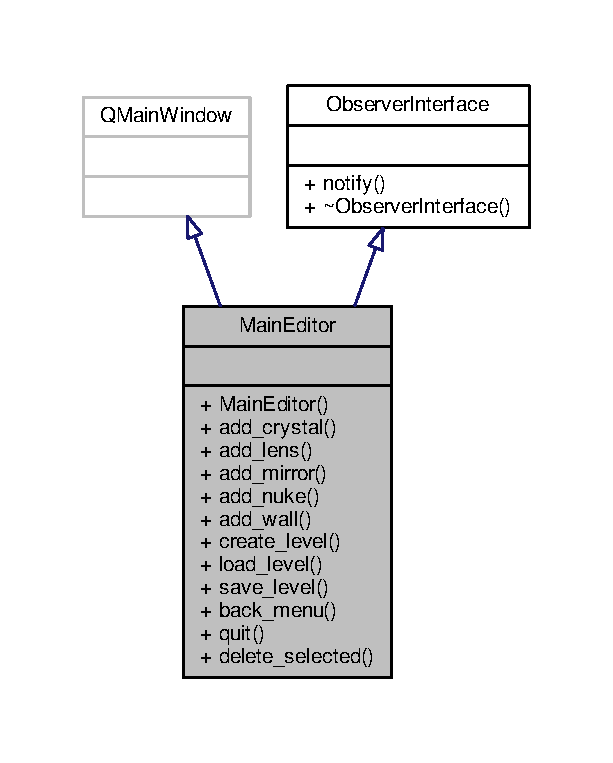
\includegraphics[width=273pt]{d1/d27/classMainEditor__inherit__graph}
\end{center}
\end{figure}


Graphe de collaboration de Main\+Editor\+:\nopagebreak
\begin{figure}[H]
\begin{center}
\leavevmode
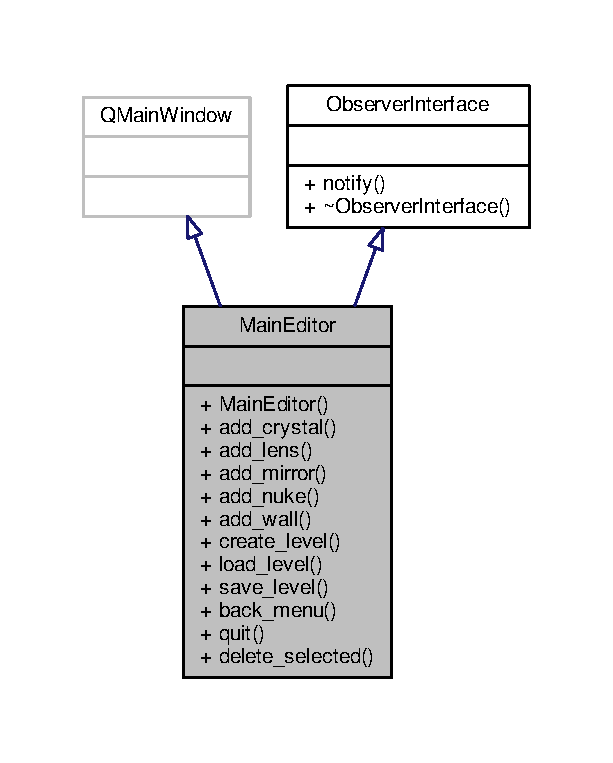
\includegraphics[width=273pt]{db/d11/classMainEditor__coll__graph}
\end{center}
\end{figure}
\subsection*{Connecteurs publics}
\begin{DoxyCompactItemize}
\item 
\hypertarget{classMainEditor_a11c01691ed4e4385c40ded07b2a4044e}{void {\bfseries add\+\_\+crystal} ()}\label{classMainEditor_a11c01691ed4e4385c40ded07b2a4044e}

\item 
\hypertarget{classMainEditor_a9cc5457b86afb73a672f12d8915082c7}{void {\bfseries add\+\_\+lens} ()}\label{classMainEditor_a9cc5457b86afb73a672f12d8915082c7}

\item 
\hypertarget{classMainEditor_a3ea0d26648a2a91f4c51fd78d06c4bd7}{void {\bfseries add\+\_\+mirror} ()}\label{classMainEditor_a3ea0d26648a2a91f4c51fd78d06c4bd7}

\item 
\hypertarget{classMainEditor_ac1563d2cb8788295cea11a3d4f668f1e}{void {\bfseries add\+\_\+nuke} ()}\label{classMainEditor_ac1563d2cb8788295cea11a3d4f668f1e}

\item 
\hypertarget{classMainEditor_a2212ba27b33fa70c0b45e3d58d784c1e}{void {\bfseries add\+\_\+wall} ()}\label{classMainEditor_a2212ba27b33fa70c0b45e3d58d784c1e}

\item 
\hypertarget{classMainEditor_a53ba9857e08e47f075487fff2c07f88e}{void {\bfseries create\+\_\+level} ()}\label{classMainEditor_a53ba9857e08e47f075487fff2c07f88e}

\item 
\hypertarget{classMainEditor_a84fe185f03ff8984471380206607e2a1}{void {\bfseries load\+\_\+level} ()}\label{classMainEditor_a84fe185f03ff8984471380206607e2a1}

\item 
\hypertarget{classMainEditor_a21dcf035be9044cd0e4677761f778505}{void {\bfseries save\+\_\+level} ()}\label{classMainEditor_a21dcf035be9044cd0e4677761f778505}

\item 
\hypertarget{classMainEditor_a41d9558029b00e6af70b67b2ef6b2abd}{void {\bfseries back\+\_\+menu} ()}\label{classMainEditor_a41d9558029b00e6af70b67b2ef6b2abd}

\item 
\hypertarget{classMainEditor_a2ad5e523c18fb96ce38616145b1b050e}{void {\bfseries quit} ()}\label{classMainEditor_a2ad5e523c18fb96ce38616145b1b050e}

\item 
\hypertarget{classMainEditor_a171515374a86a6bb81af0f34a4857cb3}{void {\bfseries delete\+\_\+selected} ()}\label{classMainEditor_a171515374a86a6bb81af0f34a4857cb3}

\end{DoxyCompactItemize}
\subsection*{Fonctions membres publiques}
\begin{DoxyCompactItemize}
\item 
\hypertarget{classMainEditor_a58a308ba8043e53ea5525e87540b0a71}{{\bfseries Main\+Editor} (Q\+Widget $\ast$parent=0)}\label{classMainEditor_a58a308ba8043e53ea5525e87540b0a71}

\end{DoxyCompactItemize}


\subsection{Description détaillée}
Fenêtre principale de l’éditeur. 

La documentation de cette classe a été générée à partir des fichiers suivants \+:\begin{DoxyCompactItemize}
\item 
editor/maineditor.\+h\item 
editor/maineditor.\+cpp\end{DoxyCompactItemize}

\hypertarget{classMainMenu}{\section{Référence de la classe Main\+Menu}
\label{classMainMenu}\index{Main\+Menu@{Main\+Menu}}
}


Graphe d'héritage de Main\+Menu\+:
\nopagebreak
\begin{figure}[H]
\begin{center}
\leavevmode
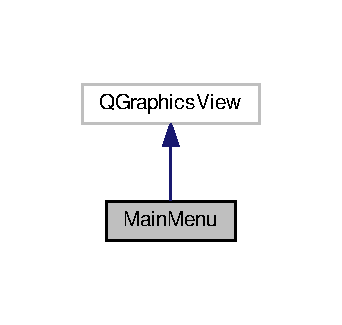
\includegraphics[width=164pt]{db/d55/classMainMenu__inherit__graph}
\end{center}
\end{figure}


Graphe de collaboration de Main\+Menu\+:
\nopagebreak
\begin{figure}[H]
\begin{center}
\leavevmode
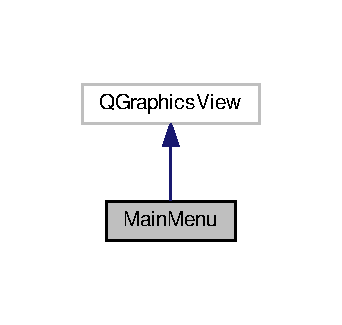
\includegraphics[width=164pt]{d8/d60/classMainMenu__coll__graph}
\end{center}
\end{figure}
\subsection*{Connecteurs publics}
\begin{DoxyCompactItemize}
\item 
\hypertarget{classMainMenu_af13a5defbd470cb18edc59d14668aaf4}{void {\bfseries start} ()}\label{classMainMenu_af13a5defbd470cb18edc59d14668aaf4}

\item 
\hypertarget{classMainMenu_aea2e199d621268d691f1aebb7a8f2e31}{void {\bfseries help} ()}\label{classMainMenu_aea2e199d621268d691f1aebb7a8f2e31}

\item 
\hypertarget{classMainMenu_adbce95d3c2192a684d25e6bf2417f073}{void {\bfseries editor} ()}\label{classMainMenu_adbce95d3c2192a684d25e6bf2417f073}

\end{DoxyCompactItemize}
\subsection*{Fonctions membres publiques}
\begin{DoxyCompactItemize}
\item 
\hypertarget{classMainMenu_a15507d68640fd9651dae4a6e3cf9b870}{{\bfseries Main\+Menu} (Q\+Widget $\ast$parent=N\+U\+L\+L)}\label{classMainMenu_a15507d68640fd9651dae4a6e3cf9b870}

\item 
\hypertarget{classMainMenu_a4b83847fe6109626f6dd4404c8afe4b2}{void {\bfseries display\+Main\+Menu} ()}\label{classMainMenu_a4b83847fe6109626f6dd4404c8afe4b2}

\end{DoxyCompactItemize}


La documentation de cette classe a été générée à partir des fichiers suivants \+:\begin{DoxyCompactItemize}
\item 
view/mainmenu.\+h\item 
view/mainmenu.\+cpp\end{DoxyCompactItemize}

\hypertarget{classMainWindow}{\section{Référence de la classe Main\+Window}
\label{classMainWindow}\index{Main\+Window@{Main\+Window}}
}


Représente la fenêtre principale.  




{\ttfamily \#include $<$mainwindow.\+h$>$}



Graphe d'héritage de Main\+Window\+:\nopagebreak
\begin{figure}[H]
\begin{center}
\leavevmode
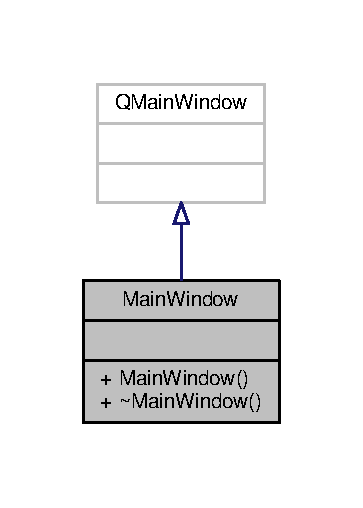
\includegraphics[width=160pt]{d1/d96/classMainWindow__inherit__graph}
\end{center}
\end{figure}


Graphe de collaboration de Main\+Window\+:\nopagebreak
\begin{figure}[H]
\begin{center}
\leavevmode
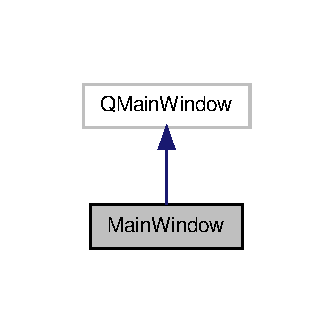
\includegraphics[width=160pt]{d2/d38/classMainWindow__coll__graph}
\end{center}
\end{figure}
\subsection*{Fonctions membres publiques}
\begin{DoxyCompactItemize}
\item 
\hypertarget{classMainWindow_a8b244be8b7b7db1b08de2a2acb9409db}{{\bfseries Main\+Window} (Q\+Widget $\ast$parent=0)}\label{classMainWindow_a8b244be8b7b7db1b08de2a2acb9409db}

\end{DoxyCompactItemize}


\subsection{Description détaillée}
Représente la fenêtre principale. 

La documentation de cette classe a été générée à partir des fichiers suivants \+:\begin{DoxyCompactItemize}
\item 
view/mainwindow.\+h\item 
view/mainwindow.\+cpp\end{DoxyCompactItemize}

\hypertarget{classMapReader}{\section{Référence de la classe Map\+Reader}
\label{classMapReader}\index{Map\+Reader@{Map\+Reader}}
}


Classe permettant de lire un fichier .lvl et d'instancier un niveau.  




{\ttfamily \#include $<$mapreader.\+h$>$}

\subsection*{Fonctions membres publiques statiques}
\begin{DoxyCompactItemize}
\item 
static \hyperlink{classLevel}{Level} $\ast$ \hyperlink{classMapReader_ac46cce595afc102320f6e73bb0748761}{level} (std\+::string path)
\begin{DoxyCompactList}\small\item\em Retourne le niveau correspondant au fichier. \end{DoxyCompactList}\item 
\hypertarget{classMapReader_afd2685d46bd9a935bf2c80a0c651898e}{static void \hyperlink{classMapReader_afd2685d46bd9a935bf2c80a0c651898e}{end\+\_\+level} ()}\label{classMapReader_afd2685d46bd9a935bf2c80a0c651898e}

\begin{DoxyCompactList}\small\item\em Supprime le niveau correspondant au fichier lu précédemment. \end{DoxyCompactList}\end{DoxyCompactItemize}


\subsection{Description détaillée}
Classe permettant de lire un fichier .lvl et d'instancier un niveau. 

\subsection{Documentation des fonctions membres}
\hypertarget{classMapReader_ac46cce595afc102320f6e73bb0748761}{\index{Map\+Reader@{Map\+Reader}!level@{level}}
\index{level@{level}!Map\+Reader@{Map\+Reader}}
\subsubsection[{level}]{\setlength{\rightskip}{0pt plus 5cm}{\bf Level} $\ast$ Map\+Reader\+::level (
\begin{DoxyParamCaption}
\item[{std\+::string}]{path}
\end{DoxyParamCaption}
)\hspace{0.3cm}{\ttfamily [static]}}}\label{classMapReader_ac46cce595afc102320f6e73bb0748761}


Retourne le niveau correspondant au fichier. 


\begin{DoxyParams}{Paramètres}
{\em path} & le chemin et nom du fichier. \\
\hline
\end{DoxyParams}
\begin{DoxyReturn}{Renvoie}
le niveau correspondant. 
\end{DoxyReturn}


La documentation de cette classe a été générée à partir des fichiers suivants \+:\begin{DoxyCompactItemize}
\item 
utils/mapreader.\+h\item 
utils/mapreader.\+cpp\end{DoxyCompactItemize}

\hypertarget{classMapView}{\section{Référence de la classe Map\+View}
\label{classMapView}\index{Map\+View@{Map\+View}}
}


Modélisation visuelle d’un plateau de jeu.  




{\ttfamily \#include $<$mapview.\+h$>$}



Graphe d'héritage de Map\+View\+:\nopagebreak
\begin{figure}[H]
\begin{center}
\leavevmode
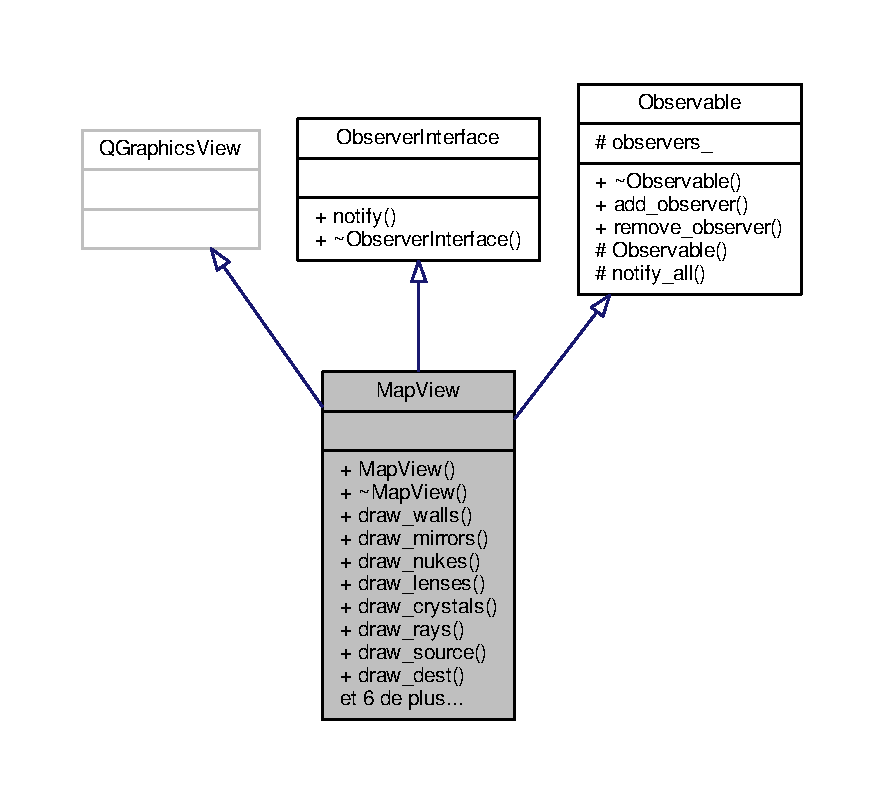
\includegraphics[width=350pt]{d6/d58/classMapView__inherit__graph}
\end{center}
\end{figure}


Graphe de collaboration de Map\+View\+:\nopagebreak
\begin{figure}[H]
\begin{center}
\leavevmode
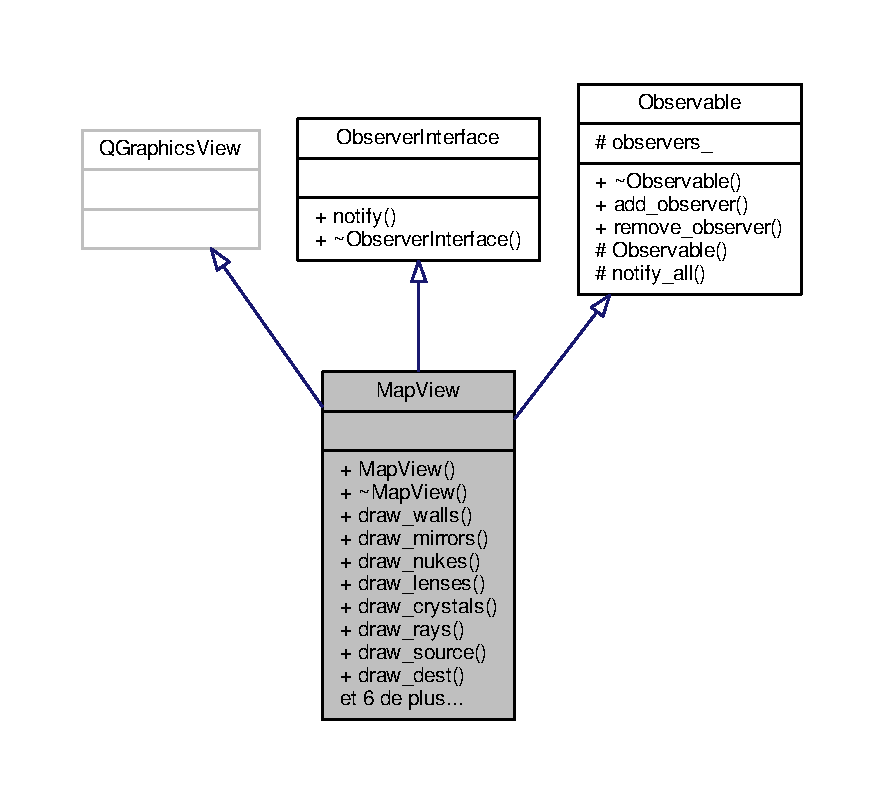
\includegraphics[width=350pt]{d1/d7b/classMapView__coll__graph}
\end{center}
\end{figure}
\subsection*{Fonctions membres publiques}
\begin{DoxyCompactItemize}
\item 
\hypertarget{classMapView_af0587bbc403c323417ea227d247c02c6}{{\bfseries Map\+View} (\hyperlink{classLevel}{Level} $\ast$level\+\_\+, bool selectable=false)}\label{classMapView_af0587bbc403c323417ea227d247c02c6}

\item 
\hypertarget{classMapView_a9243e834166e90fd20bba175fa56a4cc}{void {\bfseries draw\+\_\+walls} ()}\label{classMapView_a9243e834166e90fd20bba175fa56a4cc}

\item 
\hypertarget{classMapView_abb3bba1e54932fc2b64406995881c4ad}{void {\bfseries draw\+\_\+mirrors} ()}\label{classMapView_abb3bba1e54932fc2b64406995881c4ad}

\item 
\hypertarget{classMapView_aafe3dc35cb0938ae7e778b3ddbaf0d87}{void {\bfseries draw\+\_\+nukes} ()}\label{classMapView_aafe3dc35cb0938ae7e778b3ddbaf0d87}

\item 
\hypertarget{classMapView_a636b68282c90dab40dba5984acae2605}{void {\bfseries draw\+\_\+lenses} ()}\label{classMapView_a636b68282c90dab40dba5984acae2605}

\item 
\hypertarget{classMapView_a69e182926c3faeccd627740329451091}{void {\bfseries draw\+\_\+crystals} ()}\label{classMapView_a69e182926c3faeccd627740329451091}

\item 
\hypertarget{classMapView_a47460ba6134d7b9b0f696de8f4f6aa8a}{void {\bfseries draw\+\_\+rays} ()}\label{classMapView_a47460ba6134d7b9b0f696de8f4f6aa8a}

\item 
\hypertarget{classMapView_a7673cc6dc5da8a4312d4588bc3d8b8d0}{void {\bfseries draw\+\_\+source} ()}\label{classMapView_a7673cc6dc5da8a4312d4588bc3d8b8d0}

\item 
\hypertarget{classMapView_afffa3910baaace753c00ce187fd7115a}{void {\bfseries draw\+\_\+dest} ()}\label{classMapView_afffa3910baaace753c00ce187fd7115a}

\item 
\hypertarget{classMapView_a7e354e304c2f0135103a8773a8a8e0d4}{void {\bfseries repaint} ()}\label{classMapView_a7e354e304c2f0135103a8773a8a8e0d4}

\item 
\hypertarget{classMapView_a1c41de9351ee9f91008be7a201a3a99c}{void {\bfseries clear} ()}\label{classMapView_a1c41de9351ee9f91008be7a201a3a99c}

\item 
\hypertarget{classMapView_ab1af933413ea299a5f6d735561623471}{\hyperlink{classElementView}{Element\+View} $\ast$ {\bfseries selected} ()}\label{classMapView_ab1af933413ea299a5f6d735561623471}

\item 
\hypertarget{classMapView_aba384cd40d1f62de22ca5b3af9218656}{void {\bfseries mouse\+Press\+Event} (Q\+Mouse\+Event $\ast$event)}\label{classMapView_aba384cd40d1f62de22ca5b3af9218656}

\item 
\hypertarget{classMapView_aab858f1281826a9b9b992ecd1809127a}{void {\bfseries key\+Press\+Event} (Q\+Key\+Event $\ast$event)}\label{classMapView_aab858f1281826a9b9b992ecd1809127a}

\item 
void \hyperlink{classMapView_ac350f8c6a05f696934268a3584b53a44}{notify} (\hyperlink{classObservable}{Observable} $\ast$sdo, std\+::string msg, const std\+::vector$<$ std\+::string $>$ \&args=std\+::vector$<$ std\+::string $>$())
\begin{DoxyCompactList}\small\item\em Notifie le jeu d'un évènement provenant d'un sujet d'observation (\hyperlink{classObservable}{Observable}). \end{DoxyCompactList}\end{DoxyCompactItemize}
\subsection*{Membres hérités additionnels}


\subsection{Description détaillée}
Modélisation visuelle d’un plateau de jeu. 

\subsection{Documentation des fonctions membres}
\hypertarget{classMapView_ac350f8c6a05f696934268a3584b53a44}{\index{Map\+View@{Map\+View}!notify@{notify}}
\index{notify@{notify}!Map\+View@{Map\+View}}
\subsubsection[{notify}]{\setlength{\rightskip}{0pt plus 5cm}void Map\+View\+::notify (
\begin{DoxyParamCaption}
\item[{{\bf Observable} $\ast$}]{sdo, }
\item[{std\+::string}]{msg, }
\item[{const std\+::vector$<$ std\+::string $>$ \&}]{args = {\ttfamily std\+:\+:vector$<$~std\+:\+:string~$>$()}}
\end{DoxyParamCaption}
)\hspace{0.3cm}{\ttfamily [virtual]}}}\label{classMapView_ac350f8c6a05f696934268a3584b53a44}


Notifie le jeu d'un évènement provenant d'un sujet d'observation (\hyperlink{classObservable}{Observable}). 


\begin{DoxyParams}{Paramètres}
{\em o} & l'observé. \\
\hline
{\em msg} & le message de notification. \\
\hline
{\em args} & des arguments. \\
\hline
\end{DoxyParams}


Implémente \hyperlink{classObserverInterface_a1bbd22519c2942d978804714db12c8b2}{Observer\+Interface}.



La documentation de cette classe a été générée à partir des fichiers suivants \+:\begin{DoxyCompactItemize}
\item 
view/mapview.\+h\item 
view/mapview.\+cpp\end{DoxyCompactItemize}

\hypertarget{classMapWriter}{\section{Référence de la classe Map\+Writer}
\label{classMapWriter}\index{Map\+Writer@{Map\+Writer}}
}


Classe permettant d'écrire un niveau dans un fichier .lvl.  




{\ttfamily \#include $<$mapwriter.\+h$>$}



Graphe de collaboration de Map\+Writer\+:\nopagebreak
\begin{figure}[H]
\begin{center}
\leavevmode
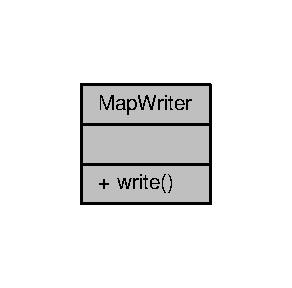
\includegraphics[width=140pt]{df/d0c/classMapWriter__coll__graph}
\end{center}
\end{figure}
\subsection*{Fonctions membres publiques statiques}
\begin{DoxyCompactItemize}
\item 
static void \hyperlink{classMapWriter_a39b4a6bb724070674f8dc2014b2f165a}{write} (const \hyperlink{classLevel}{Level} $\ast$level, const std\+::string \&path)
\begin{DoxyCompactList}\small\item\em Crée / écrit dans un fichier toutes les caractéristiques d'un niveau. \end{DoxyCompactList}\end{DoxyCompactItemize}


\subsection{Description détaillée}
Classe permettant d'écrire un niveau dans un fichier .lvl. 

\subsection{Documentation des fonctions membres}
\hypertarget{classMapWriter_a39b4a6bb724070674f8dc2014b2f165a}{\index{Map\+Writer@{Map\+Writer}!write@{write}}
\index{write@{write}!Map\+Writer@{Map\+Writer}}
\subsubsection[{write}]{\setlength{\rightskip}{0pt plus 5cm}void Map\+Writer\+::write (
\begin{DoxyParamCaption}
\item[{const {\bf Level} $\ast$}]{level, }
\item[{const std\+::string \&}]{path}
\end{DoxyParamCaption}
)\hspace{0.3cm}{\ttfamily [static]}}}\label{classMapWriter_a39b4a6bb724070674f8dc2014b2f165a}


Crée / écrit dans un fichier toutes les caractéristiques d'un niveau. 


\begin{DoxyParams}{Paramètres}
{\em level} & le niveau. \\
\hline
{\em path} & le chemin et nom du fichier à écrire. \\
\hline
\end{DoxyParams}


La documentation de cette classe a été générée à partir des fichiers suivants \+:\begin{DoxyCompactItemize}
\item 
utils/mapwriter.\+h\item 
utils/mapwriter.\+cpp\end{DoxyCompactItemize}

\hypertarget{classMirror}{\section{Référence de la classe Mirror}
\label{classMirror}\index{Mirror@{Mirror}}
}


Cette classe modélise les miroirs utilisés dans le jeu.  




{\ttfamily \#include $<$mirror.\+h$>$}



Graphe d'héritage de Mirror\+:\nopagebreak
\begin{figure}[H]
\begin{center}
\leavevmode
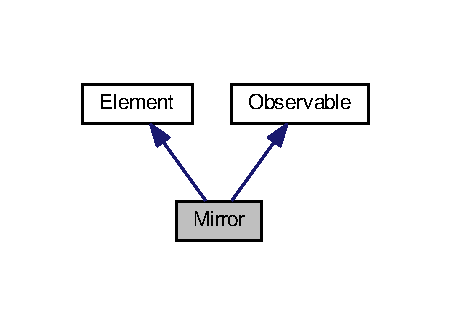
\includegraphics[width=217pt]{d8/d7d/classMirror__inherit__graph}
\end{center}
\end{figure}


Graphe de collaboration de Mirror\+:\nopagebreak
\begin{figure}[H]
\begin{center}
\leavevmode
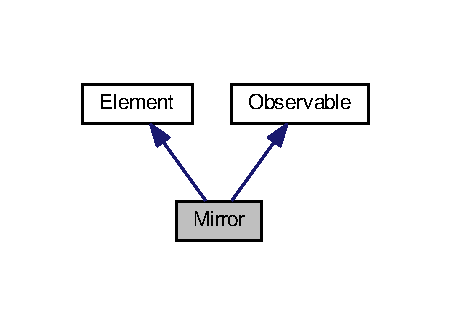
\includegraphics[width=217pt]{dc/d9b/classMirror__coll__graph}
\end{center}
\end{figure}
\subsection*{Fonctions membres publiques}
\begin{DoxyCompactItemize}
\item 
\hyperlink{classMirror_a3f32fd1e7fb4f1a3dbad8aba00d1267b}{Mirror} (const \hyperlink{classPoint}{Point} \&p, double xpad, double len, double alpha)
\begin{DoxyCompactList}\small\item\em Instancie un miroir en une position donnée, d'une certaine longueur et orienté d'un certain angle. \end{DoxyCompactList}\item 
\hyperlink{classMirror_a675db929cb6f6555163dbc2a089fe026}{Mirror} (const \hyperlink{classPoint}{Point} \&p, double xpad, double len, double alpha, const \hyperlink{classPoint}{Point} \&min, const \hyperlink{classPoint}{Point} \&max, double alpha\+\_\+min, double alpha\+\_\+max)
\begin{DoxyCompactList}\small\item\em Instancie un miroir en une position donnée, d'une certaine longueur et orienté d'un certain angle. \end{DoxyCompactList}\item 
const \hyperlink{classPoint}{Point} \& \hyperlink{classMirror_ad68e2946b5267e738663ffdf4b8841f5}{pivot} () const 
\begin{DoxyCompactList}\small\item\em Retourne la position (et le pivot) du miroir. \end{DoxyCompactList}\item 
double \hyperlink{classMirror_a9fae8ef086cb8598d689f29c68379106}{length} () const 
\begin{DoxyCompactList}\small\item\em Retourne la longueur du miroir. \end{DoxyCompactList}\item 
double \hyperlink{classMirror_aa3ec313ce158d894e084065c2eaa8cb8}{x\+\_\+pad} () const 
\begin{DoxyCompactList}\small\item\em Retourne le décalage du pivot par rapport au bord gauche du miroir. \end{DoxyCompactList}\item 
double \hyperlink{classMirror_a70b7d41a7df7213da8f8c4ac4c873739}{angle} () const 
\begin{DoxyCompactList}\small\item\em Retourne l'inclinaison du miroir. \end{DoxyCompactList}\item 
double \hyperlink{classMirror_a84dc065cb7ca7b928b83df2169021673}{min\+\_\+angle} () const 
\begin{DoxyCompactList}\small\item\em Retourne l'inclinaison minimum du miroir. \end{DoxyCompactList}\item 
double \hyperlink{classMirror_ab06cd44bc9fa2fbd942c2e021439dc1c}{max\+\_\+angle} () const 
\begin{DoxyCompactList}\small\item\em Retourne l'inclinaison maximum du miroir. \end{DoxyCompactList}\item 
\hyperlink{classPoint}{Point} \hyperlink{classMirror_ac57f542afd7fe0fd02f5b028f22821d9}{min\+\_\+pivot} () const 
\begin{DoxyCompactList}\small\item\em Retourne la position minimum du miroir. \end{DoxyCompactList}\item 
\hyperlink{classPoint}{Point} \hyperlink{classMirror_a5c7aee32ae68bcc817b996859139e909}{max\+\_\+pivot} () const 
\begin{DoxyCompactList}\small\item\em Retourne la position maximum du miroir. \end{DoxyCompactList}\item 
bool \hyperlink{classMirror_a86285a234fb321578939d3f7597bfe6d}{set\+\_\+pivot} (const \hyperlink{classPoint}{Point} \&\hyperlink{classMirror_ad68e2946b5267e738663ffdf4b8841f5}{pivot})
\begin{DoxyCompactList}\small\item\em Déplace le miroir en la position donnée, si c'est autorisé. \end{DoxyCompactList}\item 
void \hyperlink{classMirror_a5abdb9ac393b5c4e78399567bd44fc1f}{set\+\_\+xpad} (const double x)
\begin{DoxyCompactList}\small\item\em Modifie le décalage du pivot par rapport au bord gauche du miroir. \end{DoxyCompactList}\item 
void \hyperlink{classMirror_a07555306d244772a41b160e905e14af4}{set\+\_\+len} (const double len)
\begin{DoxyCompactList}\small\item\em Modifie la longueur du miroir. \end{DoxyCompactList}\item 
void \hyperlink{classMirror_a6abbc2665d17f8959191ec5b867f4d65}{set\+\_\+min} (const \hyperlink{classPoint}{Point} \&min)
\begin{DoxyCompactList}\small\item\em Modifie la position minimale du miroir. \end{DoxyCompactList}\item 
void \hyperlink{classMirror_a667e427c4d466d0a40715f5584977b53}{set\+\_\+max} (const \hyperlink{classPoint}{Point} \&max)
\begin{DoxyCompactList}\small\item\em Modifie la position maximale du miroir. \end{DoxyCompactList}\item 
void \hyperlink{classMirror_aa00abc76e86867b93f114e7cef6e07c0}{set\+\_\+alpha\+\_\+min} (const double min)
\begin{DoxyCompactList}\small\item\em Modifie l’angle d’inclinaison minimum du miroir. \end{DoxyCompactList}\item 
void \hyperlink{classMirror_a2ca09d04d47d75a7e67398563b94b6e3}{set\+\_\+alpha\+\_\+max} (const double max)
\begin{DoxyCompactList}\small\item\em Modifie l’angle d’inclinaison maximum du miroir. \end{DoxyCompactList}\item 
bool \hyperlink{classMirror_a86f8901b0db8666b98251b32ca946b5e}{set\+\_\+angle} (const double \hyperlink{classMirror_a70b7d41a7df7213da8f8c4ac4c873739}{angle})
\begin{DoxyCompactList}\small\item\em Pivote le miroir sur un angle donné, si c'est autorisé. \end{DoxyCompactList}\item 
void \hyperlink{classMirror_ae092fb48cbf523d50fa97c6b7fe149da}{set\+\_\+movable} (const bool value)
\begin{DoxyCompactList}\small\item\em Modifie le comportement du miroir. \end{DoxyCompactList}\item 
bool \hyperlink{classMirror_adb9bc206e3a5334909a70529ebdf6d09}{movable} () const 
\begin{DoxyCompactList}\small\item\em Retourne vrai si le miroir peut être déplacé ou tourné. \end{DoxyCompactList}\item 
bool \hyperlink{classMirror_a0d963145ff485dfb375d75f7f3e5bed5}{check\+\_\+angle\+\_\+range} (double \hyperlink{classMirror_a70b7d41a7df7213da8f8c4ac4c873739}{angle}) const 
\begin{DoxyCompactList}\small\item\em Retoune vrai si le miroir peut être pivoté sur l'angle donné, retourne faux sinon. \end{DoxyCompactList}\item 
bool \hyperlink{classMirror_a06a94bd486bbd4e5ed9856c0d7fb5383}{check\+\_\+pivot\+\_\+range} (const \hyperlink{classPoint}{Point} \&\hyperlink{classMirror_ad68e2946b5267e738663ffdf4b8841f5}{pivot}) const 
\begin{DoxyCompactList}\small\item\em Retoune vrai si le miroir peut être déplacé en la position donnée, retourne faux sinon. \end{DoxyCompactList}\item 
void \hyperlink{classMirror_acd55e5dae638546039a72fc3191c192c}{rotate} (double \hyperlink{classMirror_a70b7d41a7df7213da8f8c4ac4c873739}{angle})
\begin{DoxyCompactList}\small\item\em Modifie l'inclinaison de l'angle. \end{DoxyCompactList}\item 
void \hyperlink{classMirror_a6d2968b4e4baed86fa28c353feeb1a6b}{translate} (const double x, const double y)
\begin{DoxyCompactList}\small\item\em Déplace le pivot par rapport à une ordonnée et une abscisse. \end{DoxyCompactList}\item 
\hyperlink{classLineSegment}{Line\+Segment} \hyperlink{classMirror_a12183555b25eb6768af659a11054beec}{to\+\_\+line\+\_\+segment} () const 
\begin{DoxyCompactList}\small\item\em Renvoie le segment correspondant au miroir. \end{DoxyCompactList}\item 
bool \hyperlink{classMirror_a3a649dee176eabb38fb3ef4b86a94130}{operator==} (const \hyperlink{classMirror}{Mirror} \&m) const 
\begin{DoxyCompactList}\small\item\em Redéfinition de l'opérateur d'égalité. \end{DoxyCompactList}\end{DoxyCompactItemize}
\subsection*{Amis}
\begin{DoxyCompactItemize}
\item 
std\+::ostream \& \hyperlink{classMirror_a18a9b61e5b925d085bd1560fcf289b0c}{operator$<$$<$} (std\+::ostream \&out, const \hyperlink{classMirror}{Mirror} \&m)
\begin{DoxyCompactList}\small\item\em Surcharge l'opérateur de flux de sortie pour afficher un récapitulatif des caractéristiques du miroir sous-\/jacent en console. \end{DoxyCompactList}\end{DoxyCompactItemize}
\subsection*{Membres hérités additionnels}


\subsection{Description détaillée}
Cette classe modélise les miroirs utilisés dans le jeu. 

Un miroir est un segment de droite dont la propriété est de réfléchir la lumière d'un seul côté uniquement. Si un rayon lumineux touche un miroir du côté non réfléchissant, le miroir se comporte comme un mur. 

Les miroirs sont capables d'être déplacés et pivotés dans une certaine limite. 

\subsection{Documentation des constructeurs et destructeur}
\hypertarget{classMirror_a3f32fd1e7fb4f1a3dbad8aba00d1267b}{\index{Mirror@{Mirror}!Mirror@{Mirror}}
\index{Mirror@{Mirror}!Mirror@{Mirror}}
\subsubsection[{Mirror}]{\setlength{\rightskip}{0pt plus 5cm}Mirror\+::\+Mirror (
\begin{DoxyParamCaption}
\item[{const {\bf Point} \&}]{p, }
\item[{double}]{xpad, }
\item[{double}]{len, }
\item[{double}]{alpha}
\end{DoxyParamCaption}
)}}\label{classMirror_a3f32fd1e7fb4f1a3dbad8aba00d1267b}


Instancie un miroir en une position donnée, d'une certaine longueur et orienté d'un certain angle. 

Comme dans ce constructeur les limites de déplacement et de rotation du miroir ne sont pas définies, ce miroir peut se déplacer et pivoter librement. 
\begin{DoxyParams}{Paramètres}
{\em p} & la position (et le point de pivot) du miroir. \\
\hline
{\em len} & la longueur du miroir. \\
\hline
{\em x} & le décalage du pivot par rapport au bord gauche du miroir. \\
\hline
{\em a} & l'angle d'inclinaison du miroir. \\
\hline
\end{DoxyParams}
\hypertarget{classMirror_a675db929cb6f6555163dbc2a089fe026}{\index{Mirror@{Mirror}!Mirror@{Mirror}}
\index{Mirror@{Mirror}!Mirror@{Mirror}}
\subsubsection[{Mirror}]{\setlength{\rightskip}{0pt plus 5cm}Mirror\+::\+Mirror (
\begin{DoxyParamCaption}
\item[{const {\bf Point} \&}]{p, }
\item[{double}]{xpad, }
\item[{double}]{len, }
\item[{double}]{alpha, }
\item[{const {\bf Point} \&}]{min, }
\item[{const {\bf Point} \&}]{max, }
\item[{double}]{alpha\+\_\+min, }
\item[{double}]{alpha\+\_\+max}
\end{DoxyParamCaption}
)}}\label{classMirror_a675db929cb6f6555163dbc2a089fe026}


Instancie un miroir en une position donnée, d'une certaine longueur et orienté d'un certain angle. 

Ce constructeur permet également aux miroirs de pivoter dans une certaine limite. 

Si l'intervalle de limite de déplacement (e.\+g., sur les abscisses) \mbox{[}a,b\mbox{]} est tel que a = b, le miroir ne peut être déplacé sur l'axe considéré. 

Si l'intervalle de limite d'inclinaison \mbox{[}a,b\mbox{]} est tel que a $<$ b, le miroir pivote dans le sens horloger, si a = b le miroir ne peut pas pivoter, si a $>$ b, le miroir pivote dans le sens anti-\/horloger. 
\begin{DoxyParams}{Paramètres}
{\em p} & la position (et le point de pivot) du miroir. \\
\hline
{\em len} & la longueur du miroir. \\
\hline
{\em x} & le décalage du pivot par rapport au bord gauche du miroir. \\
\hline
{\em a} & l'angle d'inclinaison du miroir. \\
\hline
{\em min} & l'abscisse et l'ordonnée minimum du miroir. \\
\hline
{\em max} & l'abscisse et l'ordonnée maximum du miroir. \\
\hline
{\em amin} & l'angle d'inclinaison minimum du miroir. \\
\hline
{\em amax} & l'angle d'inclinaison maximum du miroir. \\
\hline
\end{DoxyParams}


\subsection{Documentation des fonctions membres}
\hypertarget{classMirror_a70b7d41a7df7213da8f8c4ac4c873739}{\index{Mirror@{Mirror}!angle@{angle}}
\index{angle@{angle}!Mirror@{Mirror}}
\subsubsection[{angle}]{\setlength{\rightskip}{0pt plus 5cm}double Mirror\+::angle (
\begin{DoxyParamCaption}
{}
\end{DoxyParamCaption}
) const\hspace{0.3cm}{\ttfamily [inline]}}}\label{classMirror_a70b7d41a7df7213da8f8c4ac4c873739}


Retourne l'inclinaison du miroir. 

\begin{DoxyReturn}{Renvoie}
l'inclinaison du miroir. 
\end{DoxyReturn}
\hypertarget{classMirror_a0d963145ff485dfb375d75f7f3e5bed5}{\index{Mirror@{Mirror}!check\+\_\+angle\+\_\+range@{check\+\_\+angle\+\_\+range}}
\index{check\+\_\+angle\+\_\+range@{check\+\_\+angle\+\_\+range}!Mirror@{Mirror}}
\subsubsection[{check\+\_\+angle\+\_\+range}]{\setlength{\rightskip}{0pt plus 5cm}bool Mirror\+::check\+\_\+angle\+\_\+range (
\begin{DoxyParamCaption}
\item[{double}]{angle}
\end{DoxyParamCaption}
) const}}\label{classMirror_a0d963145ff485dfb375d75f7f3e5bed5}


Retoune vrai si le miroir peut être pivoté sur l'angle donné, retourne faux sinon. 

\begin{DoxyReturn}{Renvoie}
vrai si le miroir peut être pivoté sur l'angle donné, retourne faux sinon. 
\end{DoxyReturn}
\begin{DoxySeeAlso}{Voir également}
Mirror\+::get\+Angle() 
\end{DoxySeeAlso}
\hypertarget{classMirror_a06a94bd486bbd4e5ed9856c0d7fb5383}{\index{Mirror@{Mirror}!check\+\_\+pivot\+\_\+range@{check\+\_\+pivot\+\_\+range}}
\index{check\+\_\+pivot\+\_\+range@{check\+\_\+pivot\+\_\+range}!Mirror@{Mirror}}
\subsubsection[{check\+\_\+pivot\+\_\+range}]{\setlength{\rightskip}{0pt plus 5cm}bool Mirror\+::check\+\_\+pivot\+\_\+range (
\begin{DoxyParamCaption}
\item[{const {\bf Point} \&}]{pivot}
\end{DoxyParamCaption}
) const}}\label{classMirror_a06a94bd486bbd4e5ed9856c0d7fb5383}


Retoune vrai si le miroir peut être déplacé en la position donnée, retourne faux sinon. 

\begin{DoxyReturn}{Renvoie}
vrai si le miroir peut être déplacé en la position donnée, retourne faux sinon. 
\end{DoxyReturn}
\begin{DoxySeeAlso}{Voir également}
Mirror\+::get\+Pivot() 
\end{DoxySeeAlso}
\hypertarget{classMirror_a9fae8ef086cb8598d689f29c68379106}{\index{Mirror@{Mirror}!length@{length}}
\index{length@{length}!Mirror@{Mirror}}
\subsubsection[{length}]{\setlength{\rightskip}{0pt plus 5cm}double Mirror\+::length (
\begin{DoxyParamCaption}
{}
\end{DoxyParamCaption}
) const\hspace{0.3cm}{\ttfamily [inline]}}}\label{classMirror_a9fae8ef086cb8598d689f29c68379106}


Retourne la longueur du miroir. 

\begin{DoxyReturn}{Renvoie}
la longueur du miroir 
\end{DoxyReturn}
\hypertarget{classMirror_ab06cd44bc9fa2fbd942c2e021439dc1c}{\index{Mirror@{Mirror}!max\+\_\+angle@{max\+\_\+angle}}
\index{max\+\_\+angle@{max\+\_\+angle}!Mirror@{Mirror}}
\subsubsection[{max\+\_\+angle}]{\setlength{\rightskip}{0pt plus 5cm}double Mirror\+::max\+\_\+angle (
\begin{DoxyParamCaption}
{}
\end{DoxyParamCaption}
) const\hspace{0.3cm}{\ttfamily [inline]}}}\label{classMirror_ab06cd44bc9fa2fbd942c2e021439dc1c}


Retourne l'inclinaison maximum du miroir. 

Si l'intervalle de limite d'inclinaison \mbox{[}a,b\mbox{]} est tel que a $<$ b, le miroir pivote dans le sens horloger, si a = b le miroir ne peut pas pivoter, si a $>$ b, le miroir pivote dans le sens anti-\/horloger. Si a = b = 0, le miroir peut être pialpha\+Max\+\_\+voté librement. \begin{DoxyReturn}{Renvoie}
l'inclinaison minimum du miroir. 
\end{DoxyReturn}
\hypertarget{classMirror_a5c7aee32ae68bcc817b996859139e909}{\index{Mirror@{Mirror}!max\+\_\+pivot@{max\+\_\+pivot}}
\index{max\+\_\+pivot@{max\+\_\+pivot}!Mirror@{Mirror}}
\subsubsection[{max\+\_\+pivot}]{\setlength{\rightskip}{0pt plus 5cm}{\bf Point} Mirror\+::max\+\_\+pivot (
\begin{DoxyParamCaption}
{}
\end{DoxyParamCaption}
) const\hspace{0.3cm}{\ttfamily [inline]}}}\label{classMirror_a5c7aee32ae68bcc817b996859139e909}


Retourne la position maximum du miroir. 

Si l'intervalle de limite de déplacement (e.\+g., sur les abscisses) \mbox{[}a,b\mbox{]} est tel que a = b, le miroir ne peut être déplacé sur l'axe considéré. Si a = b = 0, le miroir peut être déplacé librement. \begin{DoxyReturn}{Renvoie}
la position maximum du miroir. 
\end{DoxyReturn}
\hypertarget{classMirror_a84dc065cb7ca7b928b83df2169021673}{\index{Mirror@{Mirror}!min\+\_\+angle@{min\+\_\+angle}}
\index{min\+\_\+angle@{min\+\_\+angle}!Mirror@{Mirror}}
\subsubsection[{min\+\_\+angle}]{\setlength{\rightskip}{0pt plus 5cm}double Mirror\+::min\+\_\+angle (
\begin{DoxyParamCaption}
{}
\end{DoxyParamCaption}
) const\hspace{0.3cm}{\ttfamily [inline]}}}\label{classMirror_a84dc065cb7ca7b928b83df2169021673}


Retourne l'inclinaison minimum du miroir. 

Si l'intervalle de limite d'inclinaison \mbox{[}a,b\mbox{]} est tel que a $<$ b, le miroir pivote dans le sens horloger, si a = b le miroir ne peut pas pivoter, si a $>$ b, le miroir pivote dans le sens anti-\/horloger. Si a = b = 0, le miroir peut être pivoté librement. \begin{DoxyReturn}{Renvoie}
l'inclinaison minimum du miroir. 
\end{DoxyReturn}
\hypertarget{classMirror_ac57f542afd7fe0fd02f5b028f22821d9}{\index{Mirror@{Mirror}!min\+\_\+pivot@{min\+\_\+pivot}}
\index{min\+\_\+pivot@{min\+\_\+pivot}!Mirror@{Mirror}}
\subsubsection[{min\+\_\+pivot}]{\setlength{\rightskip}{0pt plus 5cm}{\bf Point} Mirror\+::min\+\_\+pivot (
\begin{DoxyParamCaption}
{}
\end{DoxyParamCaption}
) const\hspace{0.3cm}{\ttfamily [inline]}}}\label{classMirror_ac57f542afd7fe0fd02f5b028f22821d9}


Retourne la position minimum du miroir. 

Si l'intervalle de limite de déplacement (e.\+g., sur les abscisses) \mbox{[}a,b\mbox{]} est tel que a = b, le miroir ne peut être déplacé sur l'axe considéré. Si a = b = 0, le miroir peut être déplacé librement. \begin{DoxyReturn}{Renvoie}
la position minimum du miroir. 
\end{DoxyReturn}
\hypertarget{classMirror_adb9bc206e3a5334909a70529ebdf6d09}{\index{Mirror@{Mirror}!movable@{movable}}
\index{movable@{movable}!Mirror@{Mirror}}
\subsubsection[{movable}]{\setlength{\rightskip}{0pt plus 5cm}bool Mirror\+::movable (
\begin{DoxyParamCaption}
{}
\end{DoxyParamCaption}
) const\hspace{0.3cm}{\ttfamily [inline]}}}\label{classMirror_adb9bc206e3a5334909a70529ebdf6d09}


Retourne vrai si le miroir peut être déplacé ou tourné. 

\begin{DoxyReturn}{Renvoie}
vrai si le miroir peut être déplacé ou tourné. 
\end{DoxyReturn}
\hypertarget{classMirror_a3a649dee176eabb38fb3ef4b86a94130}{\index{Mirror@{Mirror}!operator==@{operator==}}
\index{operator==@{operator==}!Mirror@{Mirror}}
\subsubsection[{operator==}]{\setlength{\rightskip}{0pt plus 5cm}bool Mirror\+::operator== (
\begin{DoxyParamCaption}
\item[{const {\bf Mirror} \&}]{m}
\end{DoxyParamCaption}
) const}}\label{classMirror_a3a649dee176eabb38fb3ef4b86a94130}


Redéfinition de l'opérateur d'égalité. 

Retourne vrai si les mirroirs sont égaux. 
\begin{DoxyParams}{Paramètres}
{\em m} & un mirroir. \\
\hline
\end{DoxyParams}
\begin{DoxyReturn}{Renvoie}
vrai si les mirroirs sont égaux, faux sinon. 
\end{DoxyReturn}
\hypertarget{classMirror_ad68e2946b5267e738663ffdf4b8841f5}{\index{Mirror@{Mirror}!pivot@{pivot}}
\index{pivot@{pivot}!Mirror@{Mirror}}
\subsubsection[{pivot}]{\setlength{\rightskip}{0pt plus 5cm}const {\bf Point} \& Mirror\+::pivot (
\begin{DoxyParamCaption}
{}
\end{DoxyParamCaption}
) const\hspace{0.3cm}{\ttfamily [inline]}}}\label{classMirror_ad68e2946b5267e738663ffdf4b8841f5}


Retourne la position (et le pivot) du miroir. 

\begin{DoxyReturn}{Renvoie}
la position (et le pivot) du miroir. 
\end{DoxyReturn}
\hypertarget{classMirror_acd55e5dae638546039a72fc3191c192c}{\index{Mirror@{Mirror}!rotate@{rotate}}
\index{rotate@{rotate}!Mirror@{Mirror}}
\subsubsection[{rotate}]{\setlength{\rightskip}{0pt plus 5cm}void Mirror\+::rotate (
\begin{DoxyParamCaption}
\item[{double}]{angle}
\end{DoxyParamCaption}
)}}\label{classMirror_acd55e5dae638546039a72fc3191c192c}


Modifie l'inclinaison de l'angle. 


\begin{DoxyParams}{Paramètres}
{\em l'inclinaison} & à ajouter. \\
\hline
\end{DoxyParams}
\hypertarget{classMirror_a2ca09d04d47d75a7e67398563b94b6e3}{\index{Mirror@{Mirror}!set\+\_\+alpha\+\_\+max@{set\+\_\+alpha\+\_\+max}}
\index{set\+\_\+alpha\+\_\+max@{set\+\_\+alpha\+\_\+max}!Mirror@{Mirror}}
\subsubsection[{set\+\_\+alpha\+\_\+max}]{\setlength{\rightskip}{0pt plus 5cm}void Mirror\+::set\+\_\+alpha\+\_\+max (
\begin{DoxyParamCaption}
\item[{const double}]{max}
\end{DoxyParamCaption}
)\hspace{0.3cm}{\ttfamily [inline]}}}\label{classMirror_a2ca09d04d47d75a7e67398563b94b6e3}


Modifie l’angle d’inclinaison maximum du miroir. 


\begin{DoxyParams}{Paramètres}
{\em amax} & le nouvel angle d’inclinaison maximal. \\
\hline
\end{DoxyParams}
\hypertarget{classMirror_aa00abc76e86867b93f114e7cef6e07c0}{\index{Mirror@{Mirror}!set\+\_\+alpha\+\_\+min@{set\+\_\+alpha\+\_\+min}}
\index{set\+\_\+alpha\+\_\+min@{set\+\_\+alpha\+\_\+min}!Mirror@{Mirror}}
\subsubsection[{set\+\_\+alpha\+\_\+min}]{\setlength{\rightskip}{0pt plus 5cm}void Mirror\+::set\+\_\+alpha\+\_\+min (
\begin{DoxyParamCaption}
\item[{const double}]{min}
\end{DoxyParamCaption}
)\hspace{0.3cm}{\ttfamily [inline]}}}\label{classMirror_aa00abc76e86867b93f114e7cef6e07c0}


Modifie l’angle d’inclinaison minimum du miroir. 


\begin{DoxyParams}{Paramètres}
{\em amin} & le nouvel angle d’inclinaison minimal. \\
\hline
\end{DoxyParams}
\hypertarget{classMirror_a86f8901b0db8666b98251b32ca946b5e}{\index{Mirror@{Mirror}!set\+\_\+angle@{set\+\_\+angle}}
\index{set\+\_\+angle@{set\+\_\+angle}!Mirror@{Mirror}}
\subsubsection[{set\+\_\+angle}]{\setlength{\rightskip}{0pt plus 5cm}bool Mirror\+::set\+\_\+angle (
\begin{DoxyParamCaption}
\item[{const double}]{angle}
\end{DoxyParamCaption}
)\hspace{0.3cm}{\ttfamily [inline]}}}\label{classMirror_a86f8901b0db8666b98251b32ca946b5e}


Pivote le miroir sur un angle donné, si c'est autorisé. 

Retourne vrai si la rotation a été effectuée correctement, retourne faux sinon. \begin{DoxyReturn}{Renvoie}
vrai si la rotation a été effectuée correctement, retourne faux sinon. 
\end{DoxyReturn}
\begin{DoxySeeAlso}{Voir également}
Mirror\+::get\+Angle() 
\end{DoxySeeAlso}
\hypertarget{classMirror_a07555306d244772a41b160e905e14af4}{\index{Mirror@{Mirror}!set\+\_\+len@{set\+\_\+len}}
\index{set\+\_\+len@{set\+\_\+len}!Mirror@{Mirror}}
\subsubsection[{set\+\_\+len}]{\setlength{\rightskip}{0pt plus 5cm}void Mirror\+::set\+\_\+len (
\begin{DoxyParamCaption}
\item[{const double}]{len}
\end{DoxyParamCaption}
)\hspace{0.3cm}{\ttfamily [inline]}}}\label{classMirror_a07555306d244772a41b160e905e14af4}


Modifie la longueur du miroir. 


\begin{DoxyParams}{Paramètres}
{\em len} & la nouvelle longueur du miroir. \\
\hline
\end{DoxyParams}
\hypertarget{classMirror_a667e427c4d466d0a40715f5584977b53}{\index{Mirror@{Mirror}!set\+\_\+max@{set\+\_\+max}}
\index{set\+\_\+max@{set\+\_\+max}!Mirror@{Mirror}}
\subsubsection[{set\+\_\+max}]{\setlength{\rightskip}{0pt plus 5cm}void Mirror\+::set\+\_\+max (
\begin{DoxyParamCaption}
\item[{const {\bf Point} \&}]{max}
\end{DoxyParamCaption}
)\hspace{0.3cm}{\ttfamily [inline]}}}\label{classMirror_a667e427c4d466d0a40715f5584977b53}


Modifie la position maximale du miroir. 


\begin{DoxyParams}{Paramètres}
{\em x} & abscisse maximale du miroir. \\
\hline
{\em y} & ordonnée maximale du miroir. \\
\hline
\end{DoxyParams}
\hypertarget{classMirror_a6abbc2665d17f8959191ec5b867f4d65}{\index{Mirror@{Mirror}!set\+\_\+min@{set\+\_\+min}}
\index{set\+\_\+min@{set\+\_\+min}!Mirror@{Mirror}}
\subsubsection[{set\+\_\+min}]{\setlength{\rightskip}{0pt plus 5cm}void Mirror\+::set\+\_\+min (
\begin{DoxyParamCaption}
\item[{const {\bf Point} \&}]{min}
\end{DoxyParamCaption}
)\hspace{0.3cm}{\ttfamily [inline]}}}\label{classMirror_a6abbc2665d17f8959191ec5b867f4d65}


Modifie la position minimale du miroir. 


\begin{DoxyParams}{Paramètres}
{\em x} & abscisse minimale du miroir. \\
\hline
{\em y} & ordonnée minimale du miroir. \\
\hline
\end{DoxyParams}
\hypertarget{classMirror_ae092fb48cbf523d50fa97c6b7fe149da}{\index{Mirror@{Mirror}!set\+\_\+movable@{set\+\_\+movable}}
\index{set\+\_\+movable@{set\+\_\+movable}!Mirror@{Mirror}}
\subsubsection[{set\+\_\+movable}]{\setlength{\rightskip}{0pt plus 5cm}void Mirror\+::set\+\_\+movable (
\begin{DoxyParamCaption}
\item[{const bool}]{value}
\end{DoxyParamCaption}
)\hspace{0.3cm}{\ttfamily [inline]}}}\label{classMirror_ae092fb48cbf523d50fa97c6b7fe149da}


Modifie le comportement du miroir. 


\begin{DoxyParams}{Paramètres}
{\em value} & vrai si le miroir peut être déplacé ou tourné, faux sinon. \\
\hline
\end{DoxyParams}
\hypertarget{classMirror_a86285a234fb321578939d3f7597bfe6d}{\index{Mirror@{Mirror}!set\+\_\+pivot@{set\+\_\+pivot}}
\index{set\+\_\+pivot@{set\+\_\+pivot}!Mirror@{Mirror}}
\subsubsection[{set\+\_\+pivot}]{\setlength{\rightskip}{0pt plus 5cm}bool Mirror\+::set\+\_\+pivot (
\begin{DoxyParamCaption}
\item[{const {\bf Point} \&}]{pivot}
\end{DoxyParamCaption}
)\hspace{0.3cm}{\ttfamily [inline]}}}\label{classMirror_a86285a234fb321578939d3f7597bfe6d}


Déplace le miroir en la position donnée, si c'est autorisé. 

Retourne vrai si le déplacement a été effectué correctement, retourne faux sinon. \begin{DoxyReturn}{Renvoie}
vrai si le déplacement a été effectué correctement, retourne faux sinon. 
\end{DoxyReturn}
\begin{DoxySeeAlso}{Voir également}
Mirror\+::get\+Pivot() 
\end{DoxySeeAlso}
\hypertarget{classMirror_a5abdb9ac393b5c4e78399567bd44fc1f}{\index{Mirror@{Mirror}!set\+\_\+xpad@{set\+\_\+xpad}}
\index{set\+\_\+xpad@{set\+\_\+xpad}!Mirror@{Mirror}}
\subsubsection[{set\+\_\+xpad}]{\setlength{\rightskip}{0pt plus 5cm}void Mirror\+::set\+\_\+xpad (
\begin{DoxyParamCaption}
\item[{const double}]{x}
\end{DoxyParamCaption}
)\hspace{0.3cm}{\ttfamily [inline]}}}\label{classMirror_a5abdb9ac393b5c4e78399567bd44fc1f}


Modifie le décalage du pivot par rapport au bord gauche du miroir. 


\begin{DoxyParams}{Paramètres}
{\em x} & le nouveau décalage. \\
\hline
\end{DoxyParams}
\hypertarget{classMirror_a12183555b25eb6768af659a11054beec}{\index{Mirror@{Mirror}!to\+\_\+line\+\_\+segment@{to\+\_\+line\+\_\+segment}}
\index{to\+\_\+line\+\_\+segment@{to\+\_\+line\+\_\+segment}!Mirror@{Mirror}}
\subsubsection[{to\+\_\+line\+\_\+segment}]{\setlength{\rightskip}{0pt plus 5cm}{\bf Line\+Segment} Mirror\+::to\+\_\+line\+\_\+segment (
\begin{DoxyParamCaption}
{}
\end{DoxyParamCaption}
) const}}\label{classMirror_a12183555b25eb6768af659a11054beec}


Renvoie le segment correspondant au miroir. 

\begin{DoxyReturn}{Renvoie}
le segment correspondant au miroir. 
\end{DoxyReturn}
\hypertarget{classMirror_a6d2968b4e4baed86fa28c353feeb1a6b}{\index{Mirror@{Mirror}!translate@{translate}}
\index{translate@{translate}!Mirror@{Mirror}}
\subsubsection[{translate}]{\setlength{\rightskip}{0pt plus 5cm}void Mirror\+::translate (
\begin{DoxyParamCaption}
\item[{const double}]{x, }
\item[{const double}]{y}
\end{DoxyParamCaption}
)}}\label{classMirror_a6d2968b4e4baed86fa28c353feeb1a6b}


Déplace le pivot par rapport à une ordonnée et une abscisse. 


\begin{DoxyParams}{Paramètres}
{\em x} & l'abscisse. \\
\hline
{\em y} & l'ordonnée. \\
\hline
\end{DoxyParams}
\hypertarget{classMirror_aa3ec313ce158d894e084065c2eaa8cb8}{\index{Mirror@{Mirror}!x\+\_\+pad@{x\+\_\+pad}}
\index{x\+\_\+pad@{x\+\_\+pad}!Mirror@{Mirror}}
\subsubsection[{x\+\_\+pad}]{\setlength{\rightskip}{0pt plus 5cm}double Mirror\+::x\+\_\+pad (
\begin{DoxyParamCaption}
{}
\end{DoxyParamCaption}
) const\hspace{0.3cm}{\ttfamily [inline]}}}\label{classMirror_aa3ec313ce158d894e084065c2eaa8cb8}


Retourne le décalage du pivot par rapport au bord gauche du miroir. 

\begin{DoxyReturn}{Renvoie}
le décalage du pivot par rapport au bord gauche du miroir. 
\end{DoxyReturn}


\subsection{Documentation des fonctions amies et associées}
\hypertarget{classMirror_a18a9b61e5b925d085bd1560fcf289b0c}{\index{Mirror@{Mirror}!operator$<$$<$@{operator$<$$<$}}
\index{operator$<$$<$@{operator$<$$<$}!Mirror@{Mirror}}
\subsubsection[{operator$<$$<$}]{\setlength{\rightskip}{0pt plus 5cm}std\+::ostream\& operator$<$$<$ (
\begin{DoxyParamCaption}
\item[{std\+::ostream \&}]{out, }
\item[{const {\bf Mirror} \&}]{m}
\end{DoxyParamCaption}
)\hspace{0.3cm}{\ttfamily [friend]}}}\label{classMirror_a18a9b61e5b925d085bd1560fcf289b0c}


Surcharge l'opérateur de flux de sortie pour afficher un récapitulatif des caractéristiques du miroir sous-\/jacent en console. 

\begin{DoxyReturn}{Renvoie}
le flux dans lequel le miroir a été imprimé 
\end{DoxyReturn}


La documentation de cette classe a été générée à partir des fichiers suivants \+:\begin{DoxyCompactItemize}
\item 
model/mirror.\+h\item 
model/mirror.\+cpp\end{DoxyCompactItemize}

\hypertarget{classMirrorProp}{\section{Référence de la classe Mirror\+Prop}
\label{classMirrorProp}\index{Mirror\+Prop@{Mirror\+Prop}}
}


Panel permettant de modifier un miroir.  




{\ttfamily \#include $<$mirrorprop.\+h$>$}



Graphe d'héritage de Mirror\+Prop\+:
\nopagebreak
\begin{figure}[H]
\begin{center}
\leavevmode
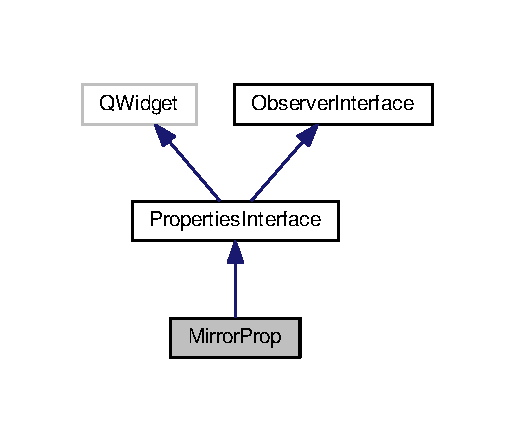
\includegraphics[width=269pt]{dc/d36/classMirrorProp__inherit__graph}
\end{center}
\end{figure}


Graphe de collaboration de Mirror\+Prop\+:
\nopagebreak
\begin{figure}[H]
\begin{center}
\leavevmode
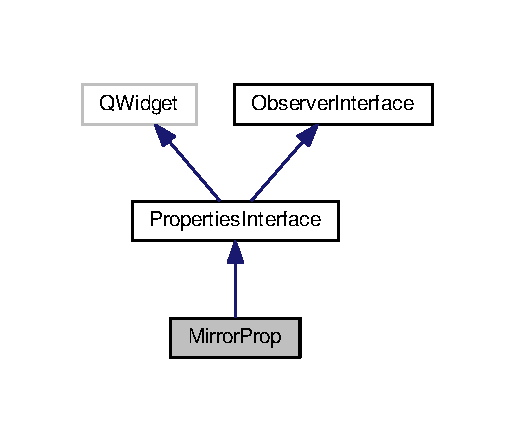
\includegraphics[width=269pt]{d3/d3c/classMirrorProp__coll__graph}
\end{center}
\end{figure}
\subsection*{Fonctions membres publiques}
\begin{DoxyCompactItemize}
\item 
\hyperlink{classMirrorProp_a66f3827e136a4de797881f58e3b2c2f5}{Mirror\+Prop} (\hyperlink{classMirror}{Mirror} $\ast$mirror, Q\+Widget $\ast$parent=0)
\begin{DoxyCompactList}\small\item\em Constructeur du widget permettant de modifier un miroir. \end{DoxyCompactList}\end{DoxyCompactItemize}


\subsection{Description détaillée}
Panel permettant de modifier un miroir. 

\subsection{Documentation des constructeurs et destructeur}
\hypertarget{classMirrorProp_a66f3827e136a4de797881f58e3b2c2f5}{\index{Mirror\+Prop@{Mirror\+Prop}!Mirror\+Prop@{Mirror\+Prop}}
\index{Mirror\+Prop@{Mirror\+Prop}!Mirror\+Prop@{Mirror\+Prop}}
\subsubsection[{Mirror\+Prop}]{\setlength{\rightskip}{0pt plus 5cm}Mirror\+Prop\+::\+Mirror\+Prop (
\begin{DoxyParamCaption}
\item[{{\bf Mirror} $\ast$}]{mirror, }
\item[{Q\+Widget $\ast$}]{parent = {\ttfamily 0}}
\end{DoxyParamCaption}
)}}\label{classMirrorProp_a66f3827e136a4de797881f58e3b2c2f5}


Constructeur du widget permettant de modifier un miroir. 


\begin{DoxyParams}{Paramètres}
{\em mirror} & le miroir à modifier. \\
\hline
{\em parent} & le widget parent. \\
\hline
\end{DoxyParams}


La documentation de cette classe a été générée à partir des fichiers suivants \+:\begin{DoxyCompactItemize}
\item 
editor/mirrorprop.\+h\item 
editor/mirrorprop.\+cpp\end{DoxyCompactItemize}

\hypertarget{classMirrorView}{\section{Référence de la classe Mirror\+View}
\label{classMirrorView}\index{Mirror\+View@{Mirror\+View}}
}


Modélisation visuelle d’un miroir.  




{\ttfamily \#include $<$mirrorview.\+h$>$}



Graphe d'héritage de Mirror\+View\+:\nopagebreak
\begin{figure}[H]
\begin{center}
\leavevmode
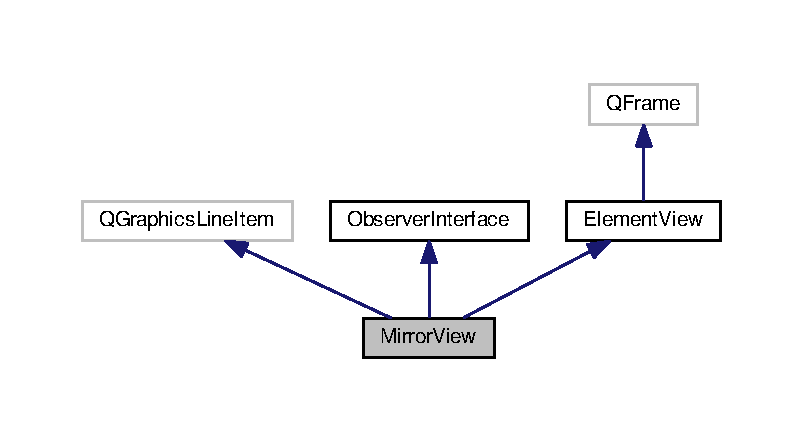
\includegraphics[width=350pt]{d2/d7b/classMirrorView__inherit__graph}
\end{center}
\end{figure}


Graphe de collaboration de Mirror\+View\+:\nopagebreak
\begin{figure}[H]
\begin{center}
\leavevmode
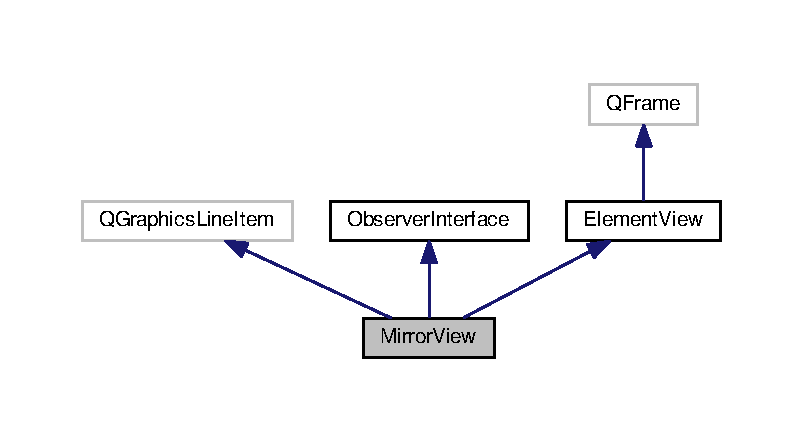
\includegraphics[width=350pt]{d1/de7/classMirrorView__coll__graph}
\end{center}
\end{figure}
\subsection*{Fonctions membres publiques}
\begin{DoxyCompactItemize}
\item 
\hyperlink{classMirrorView_a04dab41c29196186c918e60a1b2487b2}{Mirror\+View} (const \hyperlink{classMirror}{Mirror} \&\hyperlink{classMirrorView_a61c25961d7e140d5a8ff38aeb5ce8da2}{mirror}, bool selectable=false)
\begin{DoxyCompactList}\small\item\em Construit un miroir capable de refléter la lumière du rayon émis depuis la source. \end{DoxyCompactList}\item 
\hyperlink{classMirror}{Mirror} $\ast$ \hyperlink{classMirrorView_a61c25961d7e140d5a8ff38aeb5ce8da2}{mirror} ()
\begin{DoxyCompactList}\small\item\em Retourne le miroir représenté par cet objet. \end{DoxyCompactList}\item 
\hypertarget{classMirrorView_ad52e5d438a1b61b135c2ca56cadcd090}{bool {\bfseries selectable} () const }\label{classMirrorView_ad52e5d438a1b61b135c2ca56cadcd090}

\item 
\hypertarget{classMirrorView_a67fc521e337191818dba7c1abfbb6e84}{void {\bfseries set\+\_\+selectable} (bool value)}\label{classMirrorView_a67fc521e337191818dba7c1abfbb6e84}

\item 
\hypertarget{classMirrorView_ac9a758db6d2c5c99e1f5923a6248d296}{void {\bfseries show\+\_\+zone} ()}\label{classMirrorView_ac9a758db6d2c5c99e1f5923a6248d296}

\item 
\hypertarget{classMirrorView_a64fbd2447cb892fd6ffebf14a525c806}{void {\bfseries hide\+\_\+zone} ()}\label{classMirrorView_a64fbd2447cb892fd6ffebf14a525c806}

\item 
\hypertarget{classMirrorView_aaff1fd052baf4a65b6c99e75889f3705}{void {\bfseries translate} (double x=.\+0, double y=.\+0)}\label{classMirrorView_aaff1fd052baf4a65b6c99e75889f3705}

\item 
\hypertarget{classMirrorView_aaf32c32a640e6a13e92efe3f91292ad6}{void {\bfseries rotate} (double angle)}\label{classMirrorView_aaf32c32a640e6a13e92efe3f91292ad6}

\item 
void \hyperlink{classMirrorView_a5a44e12f257cb45a9f1fcc2104c08499}{notify} (\hyperlink{classObservable}{Observable} $\ast$obs, std\+::string msg, const std\+::vector$<$ std\+::string $>$ \&args=std\+::vector$<$ std\+::string $>$())
\begin{DoxyCompactList}\small\item\em Notifie le jeu d'un évènement provenant d'un sujet d'observation (\hyperlink{classObservable}{Observable}). \end{DoxyCompactList}\end{DoxyCompactItemize}
\subsection*{Membres hérités additionnels}


\subsection{Description détaillée}
Modélisation visuelle d’un miroir. 

\subsection{Documentation des constructeurs et destructeur}
\hypertarget{classMirrorView_a04dab41c29196186c918e60a1b2487b2}{\index{Mirror\+View@{Mirror\+View}!Mirror\+View@{Mirror\+View}}
\index{Mirror\+View@{Mirror\+View}!Mirror\+View@{Mirror\+View}}
\subsubsection[{Mirror\+View}]{\setlength{\rightskip}{0pt plus 5cm}Mirror\+View\+::\+Mirror\+View (
\begin{DoxyParamCaption}
\item[{const {\bf Mirror} \&}]{mirror, }
\item[{bool}]{selectable = {\ttfamily false}}
\end{DoxyParamCaption}
)}}\label{classMirrorView_a04dab41c29196186c918e60a1b2487b2}


Construit un miroir capable de refléter la lumière du rayon émis depuis la source. 


\begin{DoxyParams}{Paramètres}
{\em pivot\+X} & abscisse du pivot du miroir. \\
\hline
{\em pivot\+Y} & ordonnée du pivot du miroir. \\
\hline
{\em xpad} & distance entre le pivot et l’extrémité gauche du miroir. \\
\hline
{\em len} & longueur totale du miroir. \\
\hline
{\em angle} & angle d’inclinaison du miroir. \\
\hline
\end{DoxyParams}


\subsection{Documentation des fonctions membres}
\hypertarget{classMirrorView_a61c25961d7e140d5a8ff38aeb5ce8da2}{\index{Mirror\+View@{Mirror\+View}!mirror@{mirror}}
\index{mirror@{mirror}!Mirror\+View@{Mirror\+View}}
\subsubsection[{mirror}]{\setlength{\rightskip}{0pt plus 5cm}{\bf Mirror} $\ast$ Mirror\+View\+::mirror (
\begin{DoxyParamCaption}
{}
\end{DoxyParamCaption}
)\hspace{0.3cm}{\ttfamily [inline]}}}\label{classMirrorView_a61c25961d7e140d5a8ff38aeb5ce8da2}


Retourne le miroir représenté par cet objet. 

\begin{DoxyReturn}{Renvoie}
le miroir représenté par cet objet. 
\end{DoxyReturn}
\hypertarget{classMirrorView_a5a44e12f257cb45a9f1fcc2104c08499}{\index{Mirror\+View@{Mirror\+View}!notify@{notify}}
\index{notify@{notify}!Mirror\+View@{Mirror\+View}}
\subsubsection[{notify}]{\setlength{\rightskip}{0pt plus 5cm}void Mirror\+View\+::notify (
\begin{DoxyParamCaption}
\item[{{\bf Observable} $\ast$}]{sdo, }
\item[{std\+::string}]{msg, }
\item[{const std\+::vector$<$ std\+::string $>$ \&}]{args = {\ttfamily std\+:\+:vector$<$~std\+:\+:string~$>$()}}
\end{DoxyParamCaption}
)\hspace{0.3cm}{\ttfamily [virtual]}}}\label{classMirrorView_a5a44e12f257cb45a9f1fcc2104c08499}


Notifie le jeu d'un évènement provenant d'un sujet d'observation (\hyperlink{classObservable}{Observable}). 


\begin{DoxyParams}{Paramètres}
{\em o} & l'observé. \\
\hline
{\em msg} & le message de notification. \\
\hline
{\em args} & des arguments. \\
\hline
\end{DoxyParams}


Implémente \hyperlink{classObserverInterface_a1bbd22519c2942d978804714db12c8b2}{Observer\+Interface}.



La documentation de cette classe a été générée à partir des fichiers suivants \+:\begin{DoxyCompactItemize}
\item 
view/mirrorview.\+h\item 
view/mirrorview.\+cpp\end{DoxyCompactItemize}

\hypertarget{classNuke}{\section{Référence de la classe Nuke}
\label{classNuke}\index{Nuke@{Nuke}}
}


Cette classe modélise les bombes utilisées dans le jeu.  




{\ttfamily \#include $<$nuke.\+h$>$}



Graphe d'héritage de Nuke\+:\nopagebreak
\begin{figure}[H]
\begin{center}
\leavevmode
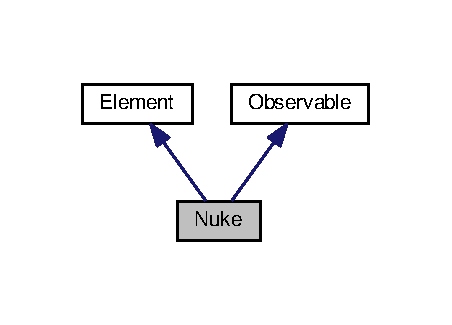
\includegraphics[width=217pt]{d7/d17/classNuke__inherit__graph}
\end{center}
\end{figure}


Graphe de collaboration de Nuke\+:\nopagebreak
\begin{figure}[H]
\begin{center}
\leavevmode
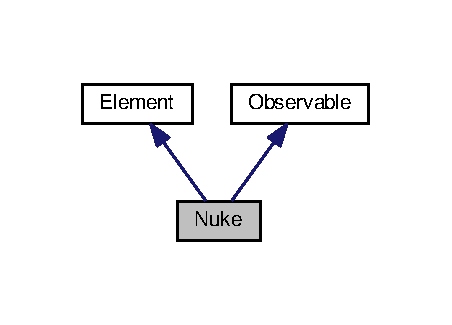
\includegraphics[width=217pt]{dc/d8c/classNuke__coll__graph}
\end{center}
\end{figure}
\subsection*{Fonctions membres publiques}
\begin{DoxyCompactItemize}
\item 
\hyperlink{classNuke_aaa149002891655e65eb870a681d1e94b}{Nuke} (const \hyperlink{classPoint}{Point} \&p, double r)
\begin{DoxyCompactList}\small\item\em Instancie une bombe en une position donnée avec un rayon déterminé. \end{DoxyCompactList}\item 
const \hyperlink{classPoint}{Point} \& \hyperlink{classNuke_a34bb8174851ffa14d5d0f9d891d59dbb}{position} () const 
\begin{DoxyCompactList}\small\item\em Retourne la position de la bombe. \end{DoxyCompactList}\item 
double \hyperlink{classNuke_af3ca35e705178487be9005d5586892b2}{radius} () const 
\begin{DoxyCompactList}\small\item\em Retourne le rayon de la bombe. \end{DoxyCompactList}\item 
bool \hyperlink{classNuke_a27bece8a254df670b90755f42a8d9bb4}{lighted\+\_\+up} () const 
\begin{DoxyCompactList}\small\item\em Retourne vrai si la bombe est illuminée, faux sinon. \end{DoxyCompactList}\item 
void \hyperlink{classNuke_a06abcff72700c24168c5779ed8b2cede}{set\+\_\+lighted\+\_\+up} (bool q)
\begin{DoxyCompactList}\small\item\em Illumine la bombe ou non. \end{DoxyCompactList}\item 
void \hyperlink{classNuke_acc486ad0d5b1f348ee1146291c2ed72e}{set\+\_\+pos} (\hyperlink{classPoint}{Point} p)
\begin{DoxyCompactList}\small\item\em Modifie la position de la bombe. \end{DoxyCompactList}\item 
void \hyperlink{classNuke_a5dbc3fbb7327fefced855e7accbf71b9}{set\+\_\+radius} (double r)
\begin{DoxyCompactList}\small\item\em Modifie le rayon de la bombe. \end{DoxyCompactList}\item 
\hyperlink{classEllipse}{Ellipse} \hyperlink{classNuke_a69f5d44f026c6643a1e1460d2d3af685}{to\+\_\+ellipse} ()
\begin{DoxyCompactList}\small\item\em Renvoie l'ellipse correspondante à la bombe. \end{DoxyCompactList}\item 
void \hyperlink{classNuke_a9ee6013c36c9f905b562f5fc38b08cbe}{translate} (double x, double y)
\begin{DoxyCompactList}\small\item\em Déplace la bombe. \end{DoxyCompactList}\item 
bool \hyperlink{classNuke_a2fcd4953abc59fd87c641f6091579eab}{operator==} (const \hyperlink{classNuke}{Nuke} \&n) const 
\begin{DoxyCompactList}\small\item\em Redéfinition de l'opérateur d'égalité. \end{DoxyCompactList}\end{DoxyCompactItemize}
\subsection*{Amis}
\begin{DoxyCompactItemize}
\item 
std\+::ostream \& \hyperlink{classNuke_a9de8a2a72db7974fd22deac7ea5728a4}{operator$<$$<$} (std\+::ostream \&out, const \hyperlink{classNuke}{Nuke} \&s)
\begin{DoxyCompactList}\small\item\em Surcharge l'opérateur de flux de sortie pour afficher un récapitulatif des caractéristiques de la bombe. \end{DoxyCompactList}\end{DoxyCompactItemize}
\subsection*{Membres hérités additionnels}


\subsection{Description détaillée}
Cette classe modélise les bombes utilisées dans le jeu. 

Une bombe est un objet circulaire qui, si illuminé par un rayon, fait perdre la partie au joueur. 

\subsection{Documentation des constructeurs et destructeur}
\hypertarget{classNuke_aaa149002891655e65eb870a681d1e94b}{\index{Nuke@{Nuke}!Nuke@{Nuke}}
\index{Nuke@{Nuke}!Nuke@{Nuke}}
\subsubsection[{Nuke}]{\setlength{\rightskip}{0pt plus 5cm}Nuke\+::\+Nuke (
\begin{DoxyParamCaption}
\item[{const {\bf Point} \&}]{p, }
\item[{double}]{r}
\end{DoxyParamCaption}
)}}\label{classNuke_aaa149002891655e65eb870a681d1e94b}


Instancie une bombe en une position donnée avec un rayon déterminé. 


\begin{DoxyParams}{Paramètres}
{\em p} & la position de la bombe. \\
\hline
{\em r} & le rayon de la bombe. \\
\hline
\end{DoxyParams}


\subsection{Documentation des fonctions membres}
\hypertarget{classNuke_a27bece8a254df670b90755f42a8d9bb4}{\index{Nuke@{Nuke}!lighted\+\_\+up@{lighted\+\_\+up}}
\index{lighted\+\_\+up@{lighted\+\_\+up}!Nuke@{Nuke}}
\subsubsection[{lighted\+\_\+up}]{\setlength{\rightskip}{0pt plus 5cm}bool Nuke\+::lighted\+\_\+up (
\begin{DoxyParamCaption}
{}
\end{DoxyParamCaption}
) const\hspace{0.3cm}{\ttfamily [inline]}}}\label{classNuke_a27bece8a254df670b90755f42a8d9bb4}


Retourne vrai si la bombe est illuminée, faux sinon. 

\begin{DoxyReturn}{Renvoie}
vrai si la bombe est illuminée, faux sinon. 
\end{DoxyReturn}
\hypertarget{classNuke_a2fcd4953abc59fd87c641f6091579eab}{\index{Nuke@{Nuke}!operator==@{operator==}}
\index{operator==@{operator==}!Nuke@{Nuke}}
\subsubsection[{operator==}]{\setlength{\rightskip}{0pt plus 5cm}bool Nuke\+::operator== (
\begin{DoxyParamCaption}
\item[{const {\bf Nuke} \&}]{n}
\end{DoxyParamCaption}
) const}}\label{classNuke_a2fcd4953abc59fd87c641f6091579eab}


Redéfinition de l'opérateur d'égalité. 

Retourne vrai si les bombes sont égales, faux sinon. 
\begin{DoxyParams}{Paramètres}
{\em n} & une autre bombe. \\
\hline
\end{DoxyParams}
\begin{DoxyReturn}{Renvoie}
vrai si les bombes sont égales, faux sinon. 
\end{DoxyReturn}
\hypertarget{classNuke_a34bb8174851ffa14d5d0f9d891d59dbb}{\index{Nuke@{Nuke}!position@{position}}
\index{position@{position}!Nuke@{Nuke}}
\subsubsection[{position}]{\setlength{\rightskip}{0pt plus 5cm}const {\bf Point} \& Nuke\+::position (
\begin{DoxyParamCaption}
{}
\end{DoxyParamCaption}
) const\hspace{0.3cm}{\ttfamily [inline]}}}\label{classNuke_a34bb8174851ffa14d5d0f9d891d59dbb}


Retourne la position de la bombe. 

\begin{DoxyReturn}{Renvoie}
la position de la bombe. 
\end{DoxyReturn}
\hypertarget{classNuke_af3ca35e705178487be9005d5586892b2}{\index{Nuke@{Nuke}!radius@{radius}}
\index{radius@{radius}!Nuke@{Nuke}}
\subsubsection[{radius}]{\setlength{\rightskip}{0pt plus 5cm}double Nuke\+::radius (
\begin{DoxyParamCaption}
{}
\end{DoxyParamCaption}
) const\hspace{0.3cm}{\ttfamily [inline]}}}\label{classNuke_af3ca35e705178487be9005d5586892b2}


Retourne le rayon de la bombe. 

\begin{DoxyReturn}{Renvoie}
le rayon de la bombe. 
\end{DoxyReturn}
\hypertarget{classNuke_a06abcff72700c24168c5779ed8b2cede}{\index{Nuke@{Nuke}!set\+\_\+lighted\+\_\+up@{set\+\_\+lighted\+\_\+up}}
\index{set\+\_\+lighted\+\_\+up@{set\+\_\+lighted\+\_\+up}!Nuke@{Nuke}}
\subsubsection[{set\+\_\+lighted\+\_\+up}]{\setlength{\rightskip}{0pt plus 5cm}void Nuke\+::set\+\_\+lighted\+\_\+up (
\begin{DoxyParamCaption}
\item[{bool}]{q}
\end{DoxyParamCaption}
)\hspace{0.3cm}{\ttfamily [inline]}}}\label{classNuke_a06abcff72700c24168c5779ed8b2cede}


Illumine la bombe ou non. 


\begin{DoxyParams}{Paramètres}
{\em q} & vrai pour illuminer la bombe, faux sinon. \\
\hline
\end{DoxyParams}
\hypertarget{classNuke_acc486ad0d5b1f348ee1146291c2ed72e}{\index{Nuke@{Nuke}!set\+\_\+pos@{set\+\_\+pos}}
\index{set\+\_\+pos@{set\+\_\+pos}!Nuke@{Nuke}}
\subsubsection[{set\+\_\+pos}]{\setlength{\rightskip}{0pt plus 5cm}void Nuke\+::set\+\_\+pos (
\begin{DoxyParamCaption}
\item[{{\bf Point}}]{p}
\end{DoxyParamCaption}
)\hspace{0.3cm}{\ttfamily [inline]}}}\label{classNuke_acc486ad0d5b1f348ee1146291c2ed72e}


Modifie la position de la bombe. 


\begin{DoxyParams}{Paramètres}
{\em p} & la nouvelle position de la bombe. \\
\hline
\end{DoxyParams}
\hypertarget{classNuke_a5dbc3fbb7327fefced855e7accbf71b9}{\index{Nuke@{Nuke}!set\+\_\+radius@{set\+\_\+radius}}
\index{set\+\_\+radius@{set\+\_\+radius}!Nuke@{Nuke}}
\subsubsection[{set\+\_\+radius}]{\setlength{\rightskip}{0pt plus 5cm}void Nuke\+::set\+\_\+radius (
\begin{DoxyParamCaption}
\item[{double}]{r}
\end{DoxyParamCaption}
)\hspace{0.3cm}{\ttfamily [inline]}}}\label{classNuke_a5dbc3fbb7327fefced855e7accbf71b9}


Modifie le rayon de la bombe. 


\begin{DoxyParams}{Paramètres}
{\em r} & le nouveau rayon de la bombe. \\
\hline
\end{DoxyParams}
\hypertarget{classNuke_a69f5d44f026c6643a1e1460d2d3af685}{\index{Nuke@{Nuke}!to\+\_\+ellipse@{to\+\_\+ellipse}}
\index{to\+\_\+ellipse@{to\+\_\+ellipse}!Nuke@{Nuke}}
\subsubsection[{to\+\_\+ellipse}]{\setlength{\rightskip}{0pt plus 5cm}{\bf Ellipse} Nuke\+::to\+\_\+ellipse (
\begin{DoxyParamCaption}
{}
\end{DoxyParamCaption}
)}}\label{classNuke_a69f5d44f026c6643a1e1460d2d3af685}


Renvoie l'ellipse correspondante à la bombe. 

\begin{DoxyReturn}{Renvoie}
l'ellipse correspondante à la bombe. 
\end{DoxyReturn}
\hypertarget{classNuke_a9ee6013c36c9f905b562f5fc38b08cbe}{\index{Nuke@{Nuke}!translate@{translate}}
\index{translate@{translate}!Nuke@{Nuke}}
\subsubsection[{translate}]{\setlength{\rightskip}{0pt plus 5cm}void Nuke\+::translate (
\begin{DoxyParamCaption}
\item[{double}]{x, }
\item[{double}]{y}
\end{DoxyParamCaption}
)}}\label{classNuke_a9ee6013c36c9f905b562f5fc38b08cbe}


Déplace la bombe. 


\begin{DoxyParams}{Paramètres}
{\em x} & le déplacement sur l'axe des x. \\
\hline
{\em y} & le déplacement sur l'axe des y. \\
\hline
\end{DoxyParams}


\subsection{Documentation des fonctions amies et associées}
\hypertarget{classNuke_a9de8a2a72db7974fd22deac7ea5728a4}{\index{Nuke@{Nuke}!operator$<$$<$@{operator$<$$<$}}
\index{operator$<$$<$@{operator$<$$<$}!Nuke@{Nuke}}
\subsubsection[{operator$<$$<$}]{\setlength{\rightskip}{0pt plus 5cm}std\+::ostream\& operator$<$$<$ (
\begin{DoxyParamCaption}
\item[{std\+::ostream \&}]{out, }
\item[{const {\bf Nuke} \&}]{s}
\end{DoxyParamCaption}
)\hspace{0.3cm}{\ttfamily [friend]}}}\label{classNuke_a9de8a2a72db7974fd22deac7ea5728a4}


Surcharge l'opérateur de flux de sortie pour afficher un récapitulatif des caractéristiques de la bombe. 

sous-\/jacente en console. \begin{DoxyReturn}{Renvoie}
le flux dans lequel la bombe a été imprimée. 
\end{DoxyReturn}


La documentation de cette classe a été générée à partir des fichiers suivants \+:\begin{DoxyCompactItemize}
\item 
model/nuke.\+h\item 
model/nuke.\+cpp\end{DoxyCompactItemize}

\hypertarget{classNukeProp}{\section{Référence de la classe Nuke\+Prop}
\label{classNukeProp}\index{Nuke\+Prop@{Nuke\+Prop}}
}


Panel permettant de modifier une bombe.  




{\ttfamily \#include $<$nukeprop.\+h$>$}



Graphe d'héritage de Nuke\+Prop\+:\nopagebreak
\begin{figure}[H]
\begin{center}
\leavevmode
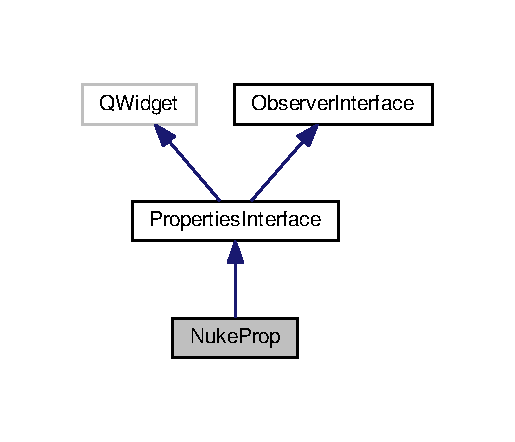
\includegraphics[width=269pt]{dc/d49/classNukeProp__inherit__graph}
\end{center}
\end{figure}


Graphe de collaboration de Nuke\+Prop\+:\nopagebreak
\begin{figure}[H]
\begin{center}
\leavevmode
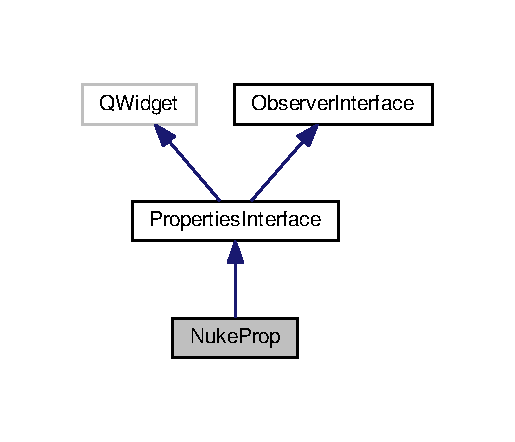
\includegraphics[width=269pt]{d0/db8/classNukeProp__coll__graph}
\end{center}
\end{figure}
\subsection*{Fonctions membres publiques}
\begin{DoxyCompactItemize}
\item 
\hypertarget{classNukeProp_a2e11beb43353c8ccbdfe1d8ba7eb61a6}{{\bfseries Nuke\+Prop} (\hyperlink{classNuke}{Nuke} $\ast$nuke, Q\+Widget $\ast$parent=0)}\label{classNukeProp_a2e11beb43353c8ccbdfe1d8ba7eb61a6}

\end{DoxyCompactItemize}


\subsection{Description détaillée}
Panel permettant de modifier une bombe. 

La documentation de cette classe a été générée à partir des fichiers suivants \+:\begin{DoxyCompactItemize}
\item 
editor/nukeprop.\+h\item 
editor/nukeprop.\+cpp\end{DoxyCompactItemize}

\hypertarget{classNukeView}{\section{Référence de la classe Nuke\+View}
\label{classNukeView}\index{Nuke\+View@{Nuke\+View}}
}


Modélisation visuelle d’une bombe.  




{\ttfamily \#include $<$nukeview.\+h$>$}



Graphe d'héritage de Nuke\+View\+:\nopagebreak
\begin{figure}[H]
\begin{center}
\leavevmode
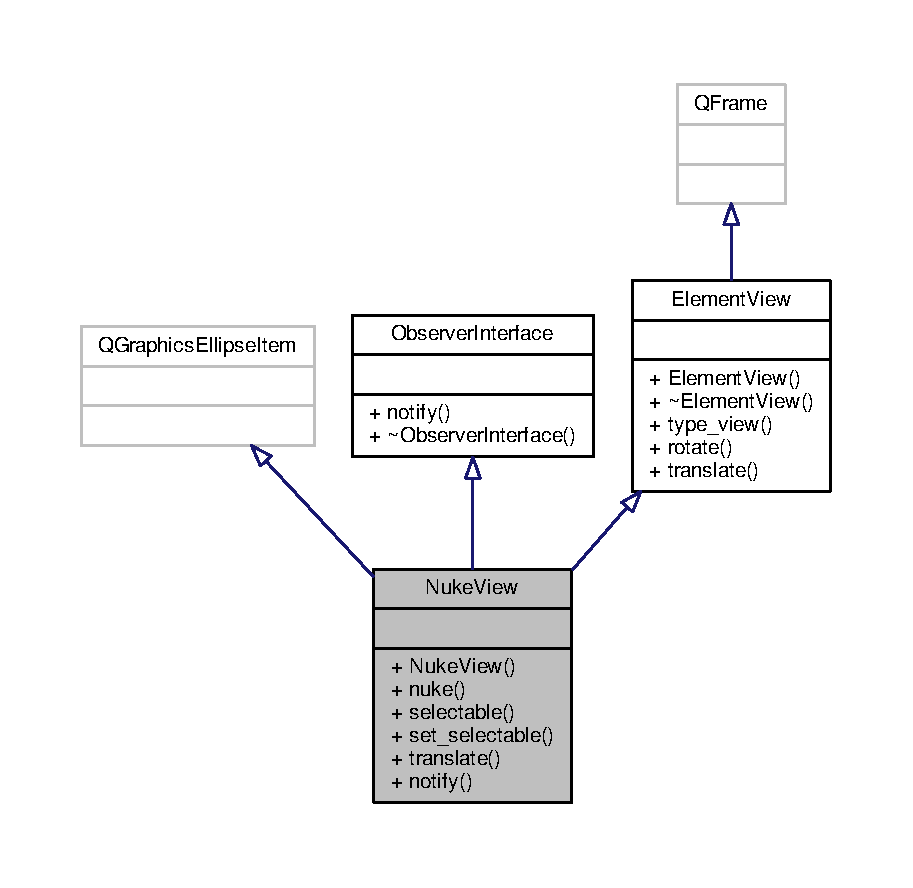
\includegraphics[width=350pt]{da/d21/classNukeView__inherit__graph}
\end{center}
\end{figure}


Graphe de collaboration de Nuke\+View\+:\nopagebreak
\begin{figure}[H]
\begin{center}
\leavevmode
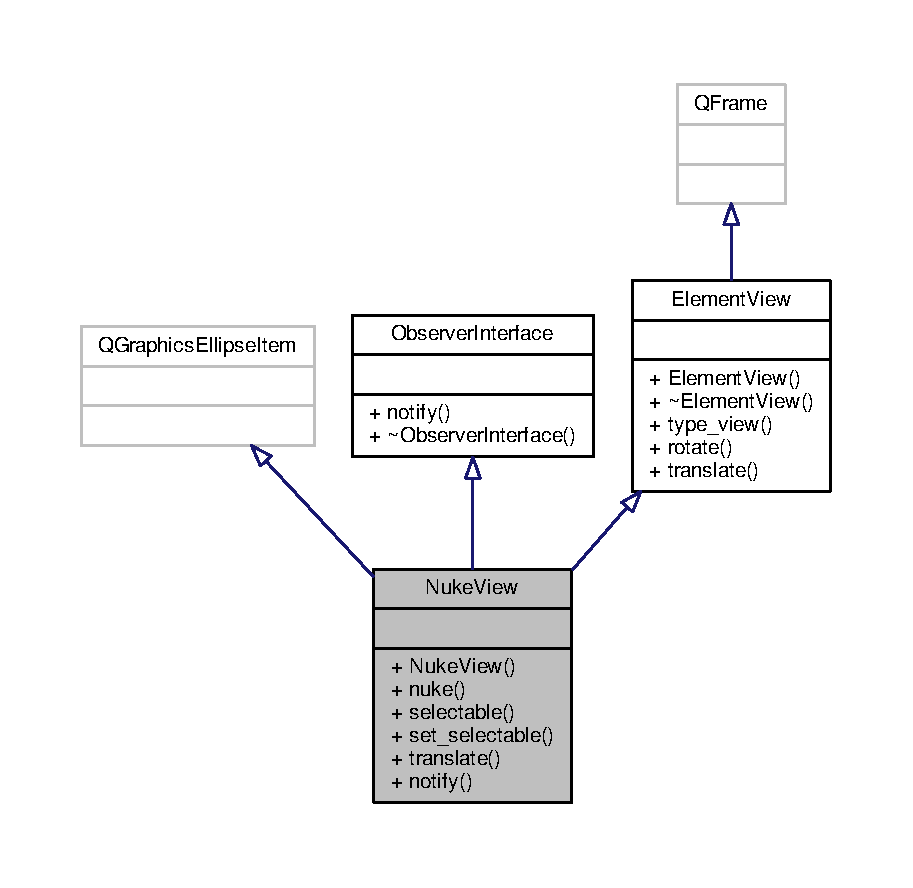
\includegraphics[width=350pt]{db/d47/classNukeView__coll__graph}
\end{center}
\end{figure}
\subsection*{Fonctions membres publiques}
\begin{DoxyCompactItemize}
\item 
\hypertarget{classNukeView_a9bb87e648efa96308058a68748e53a41}{{\bfseries Nuke\+View} (const \hyperlink{classNuke}{Nuke} \&nuke, bool selectable=false)}\label{classNukeView_a9bb87e648efa96308058a68748e53a41}

\item 
\hypertarget{classNukeView_a8bf8e524e5627138ed6c028cb4b87d2b}{\hyperlink{classNuke}{Nuke} $\ast$ {\bfseries nuke} ()}\label{classNukeView_a8bf8e524e5627138ed6c028cb4b87d2b}

\item 
\hypertarget{classNukeView_a70589619df5713cadcc47f399fae6e00}{bool {\bfseries selectable} () const }\label{classNukeView_a70589619df5713cadcc47f399fae6e00}

\item 
\hypertarget{classNukeView_ab3761858ebbe1f6dcde7813c4118bfd0}{void {\bfseries set\+\_\+selectable} (bool value)}\label{classNukeView_ab3761858ebbe1f6dcde7813c4118bfd0}

\item 
void \hyperlink{classNukeView_ab5743729fc4659e2cd670d42800c9856}{translate} (const double x=.\+0, const double y=.\+0) override
\begin{DoxyCompactList}\small\item\em Effectue une translation de l’objet sur l’axe des abscisses et des ordonnées. \end{DoxyCompactList}\item 
void \hyperlink{classNukeView_af45ef374496a0ef5b3d595ab1e5fba20}{notify} (\hyperlink{classObservable}{Observable} $\ast$o, const std\+::string \&msg, const std\+::vector$<$ std\+::string $>$ \&args) override
\begin{DoxyCompactList}\small\item\em Notifie le jeu d'un évènement provenant d'un sujet d'observation (\hyperlink{classObservable}{Observable}). \end{DoxyCompactList}\end{DoxyCompactItemize}
\subsection*{Membres hérités additionnels}


\subsection{Description détaillée}
Modélisation visuelle d’une bombe. 

\subsection{Documentation des fonctions membres}
\hypertarget{classNukeView_af45ef374496a0ef5b3d595ab1e5fba20}{\index{Nuke\+View@{Nuke\+View}!notify@{notify}}
\index{notify@{notify}!Nuke\+View@{Nuke\+View}}
\subsubsection[{notify}]{\setlength{\rightskip}{0pt plus 5cm}void Nuke\+View\+::notify (
\begin{DoxyParamCaption}
\item[{{\bf Observable} $\ast$}]{o, }
\item[{const std\+::string \&}]{msg, }
\item[{const std\+::vector$<$ std\+::string $>$ \&}]{args}
\end{DoxyParamCaption}
)\hspace{0.3cm}{\ttfamily [override]}, {\ttfamily [virtual]}}}\label{classNukeView_af45ef374496a0ef5b3d595ab1e5fba20}


Notifie le jeu d'un évènement provenant d'un sujet d'observation (\hyperlink{classObservable}{Observable}). 


\begin{DoxyParams}{Paramètres}
{\em o} & l'observé. \\
\hline
{\em msg} & le message de notification. \\
\hline
{\em args} & des arguments. \\
\hline
\end{DoxyParams}


Implémente \hyperlink{classObserverInterface_a3083639e706557f950f62af8ab283150}{Observer\+Interface}.

\hypertarget{classNukeView_ab5743729fc4659e2cd670d42800c9856}{\index{Nuke\+View@{Nuke\+View}!translate@{translate}}
\index{translate@{translate}!Nuke\+View@{Nuke\+View}}
\subsubsection[{translate}]{\setlength{\rightskip}{0pt plus 5cm}void Nuke\+View\+::translate (
\begin{DoxyParamCaption}
\item[{const double}]{x = {\ttfamily .0}, }
\item[{const double}]{y = {\ttfamily .0}}
\end{DoxyParamCaption}
)\hspace{0.3cm}{\ttfamily [override]}, {\ttfamily [virtual]}}}\label{classNukeView_ab5743729fc4659e2cd670d42800c9856}


Effectue une translation de l’objet sur l’axe des abscisses et des ordonnées. 


\begin{DoxyParams}{Paramètres}
{\em x} & la translation sur l’axe des abscisses. \\
\hline
{\em y} & la translation sur l’axe des ordonnées. \\
\hline
\end{DoxyParams}


Réimplémentée à partir de \hyperlink{classElementView_a69a525cb674a36e33be6a8b7a6e4b83c}{Element\+View}.



La documentation de cette classe a été générée à partir des fichiers suivants \+:\begin{DoxyCompactItemize}
\item 
view/nukeview.\+h\item 
view/nukeview.\+cpp\end{DoxyCompactItemize}

\hypertarget{classObservable}{\section{Référence de la classe Observable}
\label{classObservable}\index{Observable@{Observable}}
}


{\ttfamily \#include $<$observable.\+h$>$}



Graphe d'héritage de Observable\+:
\nopagebreak
\begin{figure}[H]
\begin{center}
\leavevmode
\includegraphics[width=350pt]{d7/d7e/classObservable__inherit__graph}
\end{center}
\end{figure}
\subsection*{Fonctions membres publiques}
\begin{DoxyCompactItemize}
\item 
\hypertarget{classObservable_a058acb5a674eba2b96648c66a27440d8}{virtual \hyperlink{classObservable_a058acb5a674eba2b96648c66a27440d8}{$\sim$\+Observable} ()=default}\label{classObservable_a058acb5a674eba2b96648c66a27440d8}

\begin{DoxyCompactList}\small\item\em Destructeur par défaut. \end{DoxyCompactList}\item 
virtual void \hyperlink{classObservable_a4d816915e134f1585a3f4151c6d74b1f}{add\+\_\+observer} (\hyperlink{classObserverInterface}{Observer\+Interface} $\ast$obs)
\begin{DoxyCompactList}\small\item\em Méthode permettant à un observateur de s'enregistrer comme écouteur du sujet d'observation. \end{DoxyCompactList}\item 
virtual void \hyperlink{classObservable_a79bdffc61fbea9b16d00d5bc6a2289ad}{remove\+\_\+observer} (\hyperlink{classObserverInterface}{Observer\+Interface} $\ast$obs)
\begin{DoxyCompactList}\small\item\em Méthode permettant à un observateur de se retirer de la liste des écouteurs patentés du sujet d'observation. \end{DoxyCompactList}\end{DoxyCompactItemize}
\subsection*{Fonctions membres protégées}
\begin{DoxyCompactItemize}
\item 
\hypertarget{classObservable_ab3559b2daa90b06b123089508b3d193d}{\hyperlink{classObservable_ab3559b2daa90b06b123089508b3d193d}{Observable} ()=default}\label{classObservable_ab3559b2daa90b06b123089508b3d193d}

\begin{DoxyCompactList}\small\item\em Constructeur protégé pour éviter l'instanciation. \end{DoxyCompactList}\item 
\hypertarget{classObservable_a0ea369066b16b465fa95c975cd69615a}{virtual void \hyperlink{classObservable_a0ea369066b16b465fa95c975cd69615a}{notify\+\_\+all} (std\+::string msg, const std\+::vector$<$ std\+::string $>$ \&args=std\+::vector$<$ std\+::string $>$())}\label{classObservable_a0ea369066b16b465fa95c975cd69615a}

\begin{DoxyCompactList}\small\item\em Notifie tous les observateurs enregistrés d'un changement d'état. \end{DoxyCompactList}\end{DoxyCompactItemize}
\subsection*{Attributs protégés}
\begin{DoxyCompactItemize}
\item 
\hypertarget{classObservable_aadd5f7cdec9b55bfb230771dfb77a7f3}{std\+::set$<$ \hyperlink{classObserverInterface}{Observer\+Interface} $\ast$ $>$ \hyperlink{classObservable_aadd5f7cdec9b55bfb230771dfb77a7f3}{observers\+\_\+}}\label{classObservable_aadd5f7cdec9b55bfb230771dfb77a7f3}

\begin{DoxyCompactList}\small\item\em Les observateurs enregistrés. \end{DoxyCompactList}\end{DoxyCompactItemize}


\subsection{Description détaillée}
Classe représentant un élément observable pouvant notifié des observateurs. 

\subsection{Documentation des fonctions membres}
\hypertarget{classObservable_a4d816915e134f1585a3f4151c6d74b1f}{\index{Observable@{Observable}!add\+\_\+observer@{add\+\_\+observer}}
\index{add\+\_\+observer@{add\+\_\+observer}!Observable@{Observable}}
\subsubsection[{add\+\_\+observer}]{\setlength{\rightskip}{0pt plus 5cm}void Observable\+::add\+\_\+observer (
\begin{DoxyParamCaption}
\item[{{\bf Observer\+Interface} $\ast$}]{obs}
\end{DoxyParamCaption}
)\hspace{0.3cm}{\ttfamily [virtual]}}}\label{classObservable_a4d816915e134f1585a3f4151c6d74b1f}


Méthode permettant à un observateur de s'enregistrer comme écouteur du sujet d'observation. 


\begin{DoxyParams}{Paramètres}
{\em obs} & un pointeur vers un observateur à ajouter. \\
\hline
\end{DoxyParams}
\hypertarget{classObservable_a79bdffc61fbea9b16d00d5bc6a2289ad}{\index{Observable@{Observable}!remove\+\_\+observer@{remove\+\_\+observer}}
\index{remove\+\_\+observer@{remove\+\_\+observer}!Observable@{Observable}}
\subsubsection[{remove\+\_\+observer}]{\setlength{\rightskip}{0pt plus 5cm}void Observable\+::remove\+\_\+observer (
\begin{DoxyParamCaption}
\item[{{\bf Observer\+Interface} $\ast$}]{obs}
\end{DoxyParamCaption}
)\hspace{0.3cm}{\ttfamily [virtual]}}}\label{classObservable_a79bdffc61fbea9b16d00d5bc6a2289ad}


Méthode permettant à un observateur de se retirer de la liste des écouteurs patentés du sujet d'observation. 


\begin{DoxyParams}{Paramètres}
{\em obs} & l'adresse de l'observateur à supprimer. \\
\hline
\end{DoxyParams}


La documentation de cette classe a été générée à partir des fichiers suivants \+:\begin{DoxyCompactItemize}
\item 
obs/observable.\+h\item 
obs/observable.\+cpp\end{DoxyCompactItemize}

\hypertarget{classObserverInterface}{\section{Référence de la classe Observer\+Interface}
\label{classObserverInterface}\index{Observer\+Interface@{Observer\+Interface}}
}


Interface représentant un observateur.  




{\ttfamily \#include $<$observerinterface.\+h$>$}



Graphe d'héritage de Observer\+Interface\+:
\nopagebreak
\begin{figure}[H]
\begin{center}
\leavevmode
\includegraphics[width=350pt]{d7/d5b/classObserverInterface__inherit__graph}
\end{center}
\end{figure}


Graphe de collaboration de Observer\+Interface\+:\nopagebreak
\begin{figure}[H]
\begin{center}
\leavevmode
\includegraphics[width=194pt]{d9/d44/classObserverInterface__coll__graph}
\end{center}
\end{figure}
\subsection*{Fonctions membres publiques}
\begin{DoxyCompactItemize}
\item 
virtual void \hyperlink{classObserverInterface_a3083639e706557f950f62af8ab283150}{notify} (\hyperlink{classObservable}{Observable} $\ast$o, const std\+::string \&msg, const std\+::vector$<$ std\+::string $>$ \&args=std\+::vector$<$ std\+::string $>$())=0
\begin{DoxyCompactList}\small\item\em Notifie le jeu d'un évènement provenant d'un sujet d'observation (\hyperlink{classObservable}{Observable}). \end{DoxyCompactList}\end{DoxyCompactItemize}


\subsection{Description détaillée}
Interface représentant un observateur. 

Toutes classes héritant de cette interface doit redéfinir la méthode notify. Un observateur reçoit des notifications d'une classe héritant d'\hyperlink{classObservable}{Observable}. 

\subsection{Documentation des fonctions membres}
\hypertarget{classObserverInterface_a3083639e706557f950f62af8ab283150}{\index{Observer\+Interface@{Observer\+Interface}!notify@{notify}}
\index{notify@{notify}!Observer\+Interface@{Observer\+Interface}}
\subsubsection[{notify}]{\setlength{\rightskip}{0pt plus 5cm}virtual void Observer\+Interface\+::notify (
\begin{DoxyParamCaption}
\item[{{\bf Observable} $\ast$}]{o, }
\item[{const std\+::string \&}]{msg, }
\item[{const std\+::vector$<$ std\+::string $>$ \&}]{args = {\ttfamily std\+:\+:vector$<$~std\+:\+:string~$>$()}}
\end{DoxyParamCaption}
)\hspace{0.3cm}{\ttfamily [pure virtual]}}}\label{classObserverInterface_a3083639e706557f950f62af8ab283150}


Notifie le jeu d'un évènement provenant d'un sujet d'observation (\hyperlink{classObservable}{Observable}). 


\begin{DoxyParams}{Paramètres}
{\em o} & l'observé. \\
\hline
{\em msg} & le message de notification. \\
\hline
{\em args} & des arguments. \\
\hline
\end{DoxyParams}


Implémenté dans \hyperlink{classLevel_a02cd551cc86ee390aa3559f9f2479a26}{Level}, \hyperlink{classMapView_af57740f402cad958653bdba417f87fe0}{Map\+View}, \hyperlink{classMirrorView_a20d9601e53e0b6f30a845e8ba50c96c2}{Mirror\+View}, \hyperlink{classSourceView_a615ac7a3f10992488cccf60fd89044b0}{Source\+View}, \hyperlink{classDestinationView_ad200371afdce766b4208e45d83d1ba25}{Destination\+View}, \hyperlink{classCrystalView_a6dbe86bec06d3b63182804f4f5860054}{Crystal\+View}, \hyperlink{classWallView_a68050e9027589cc7d1ab592e1cd8003c}{Wall\+View}, \hyperlink{classNukeView_af45ef374496a0ef5b3d595ab1e5fba20}{Nuke\+View}, \hyperlink{classLensView_a09506e0da9265c47140ded3e6eb35a7f}{Lens\+View}, et \hyperlink{classPropertiesInterface_a317a8df57b8387be63632a31eddb241d}{Properties\+Interface}.



La documentation de cette classe a été générée à partir du fichier suivant \+:\begin{DoxyCompactItemize}
\item 
obs/observerinterface.\+h\end{DoxyCompactItemize}

\hypertarget{classPoint}{\section{Référence de la classe Point}
\label{classPoint}\index{Point@{Point}}
}


Cette classe modélise un simple point de coordonnées réelles utilisés pour modéliser les positions des objets dans le jeu.  




{\ttfamily \#include $<$point.\+h$>$}

\subsection*{Fonctions membres publiques}
\begin{DoxyCompactItemize}
\item 
\hypertarget{classPoint_a257415ad611a16bb73628efcdb87d0fd}{\hyperlink{classPoint_a257415ad611a16bb73628efcdb87d0fd}{Point} ()=default}\label{classPoint_a257415ad611a16bb73628efcdb87d0fd}

\begin{DoxyCompactList}\small\item\em Instancie le point (0,0) \end{DoxyCompactList}\item 
\hyperlink{classPoint_a78b55e8d5466bb8c2cf60fa55f2562ff}{Point} (double \hyperlink{classPoint_a3eef47b1c4849b3395a8f9c658ca7c4a}{x}, double \hyperlink{classPoint_a96e90df6b3c18e64c31abdf196e49ae9}{y})
\begin{DoxyCompactList}\small\item\em Instancie le point de coordonnées spécifiées. \end{DoxyCompactList}\item 
\hyperlink{classPoint_af0c0f20db1616447bc78184ed537ef6e}{Point} (const \hyperlink{classPoint}{Point} \&p)
\begin{DoxyCompactList}\small\item\em Constructeur de copie. \end{DoxyCompactList}\item 
double \hyperlink{classPoint_a3eef47b1c4849b3395a8f9c658ca7c4a}{x} () const 
\begin{DoxyCompactList}\small\item\em Retourne l'abscisse du point. \end{DoxyCompactList}\item 
double \hyperlink{classPoint_a96e90df6b3c18e64c31abdf196e49ae9}{y} () const 
\begin{DoxyCompactList}\small\item\em Retourne l'ordonnée du point. \end{DoxyCompactList}\item 
void \hyperlink{classPoint_adaaf2fe64c78448b3c8d6e121ae3bca0}{set\+\_\+x} (double \hyperlink{classPoint_a3eef47b1c4849b3395a8f9c658ca7c4a}{x})
\begin{DoxyCompactList}\small\item\em Déplace le point en l'abscisse donnée. \end{DoxyCompactList}\item 
void \hyperlink{classPoint_a44bf07535f5dd99991a274833462379b}{set\+\_\+y} (double \hyperlink{classPoint_a96e90df6b3c18e64c31abdf196e49ae9}{y})
\begin{DoxyCompactList}\small\item\em Déplace le point en l'ordonnée donnée. \end{DoxyCompactList}\item 
void \hyperlink{classPoint_ad41fea4a6458fd82d9055b45d0a3c030}{set\+\_\+position} (double \hyperlink{classPoint_a3eef47b1c4849b3395a8f9c658ca7c4a}{x}, double \hyperlink{classPoint_a96e90df6b3c18e64c31abdf196e49ae9}{y})
\begin{DoxyCompactList}\small\item\em Déplace le point en la coordonnée donnée. \end{DoxyCompactList}\item 
double \hyperlink{classPoint_a61651e744a578356e2296e7935e858d7}{distance} (const \hyperlink{classPoint}{Point} \&p) const 
\begin{DoxyCompactList}\small\item\em Retourne la distance entre deux points. \end{DoxyCompactList}\item 
const \hyperlink{classPoint}{Point} \& \hyperlink{classPoint_a1436b60e581a48190621810f2a4d29cb}{operator=} (const \hyperlink{classPoint}{Point} \&p1)
\begin{DoxyCompactList}\small\item\em Surcharge de l'opérateur d'assignation. \end{DoxyCompactList}\item 
bool \hyperlink{classPoint_a2a6b68cd301437368de443687fc2a9f1}{operator==} (const \hyperlink{classPoint}{Point} \&p) const 
\begin{DoxyCompactList}\small\item\em Surcharge de l'opérateur d'égalité. \end{DoxyCompactList}\end{DoxyCompactItemize}
\subsection*{Amis}
\begin{DoxyCompactItemize}
\item 
bool \hyperlink{classPoint_aea03821811d00d0a252f7d845b3cf4a5}{operator$<$} (const \hyperlink{classPoint}{Point} \&p1, const \hyperlink{classPoint}{Point} \&p2)
\begin{DoxyCompactList}\small\item\em Redéfinit l'opérateur $<$. \end{DoxyCompactList}\item 
std\+::ostream \& \hyperlink{classPoint_aa818efa680e0d94ce91173ccb4b7aa08}{operator$<$$<$} (std\+::ostream \&out, const \hyperlink{classPoint}{Point} \&p)
\begin{DoxyCompactList}\small\item\em Surcharge l'opérateur de flux de sortie pour afficher un récapitulatif des caractéristiques du point sous-\/jacent en console. \end{DoxyCompactList}\end{DoxyCompactItemize}


\subsection{Description détaillée}
Cette classe modélise un simple point de coordonnées réelles utilisés pour modéliser les positions des objets dans le jeu. 

\subsection{Documentation des constructeurs et destructeur}
\hypertarget{classPoint_a78b55e8d5466bb8c2cf60fa55f2562ff}{\index{Point@{Point}!Point@{Point}}
\index{Point@{Point}!Point@{Point}}
\subsubsection[{Point}]{\setlength{\rightskip}{0pt plus 5cm}Point\+::\+Point (
\begin{DoxyParamCaption}
\item[{double}]{x, }
\item[{double}]{y}
\end{DoxyParamCaption}
)}}\label{classPoint_a78b55e8d5466bb8c2cf60fa55f2562ff}


Instancie le point de coordonnées spécifiées. 


\begin{DoxyParams}{Paramètres}
{\em x} & l'abscisse du point. \\
\hline
{\em y} & l'ordonnée du point. \\
\hline
\end{DoxyParams}
\hypertarget{classPoint_af0c0f20db1616447bc78184ed537ef6e}{\index{Point@{Point}!Point@{Point}}
\index{Point@{Point}!Point@{Point}}
\subsubsection[{Point}]{\setlength{\rightskip}{0pt plus 5cm}Point\+::\+Point (
\begin{DoxyParamCaption}
\item[{const {\bf Point} \&}]{p}
\end{DoxyParamCaption}
)}}\label{classPoint_af0c0f20db1616447bc78184ed537ef6e}


Constructeur de copie. 


\begin{DoxyParams}{Paramètres}
{\em p} & le point à copier. \\
\hline
\end{DoxyParams}


\subsection{Documentation des fonctions membres}
\hypertarget{classPoint_a61651e744a578356e2296e7935e858d7}{\index{Point@{Point}!distance@{distance}}
\index{distance@{distance}!Point@{Point}}
\subsubsection[{distance}]{\setlength{\rightskip}{0pt plus 5cm}double Point\+::distance (
\begin{DoxyParamCaption}
\item[{const {\bf Point} \&}]{p}
\end{DoxyParamCaption}
) const}}\label{classPoint_a61651e744a578356e2296e7935e858d7}


Retourne la distance entre deux points. 


\begin{DoxyParams}{Paramètres}
{\em p} & l'autre point avec lequel on calcule la distance. \\
\hline
\end{DoxyParams}
\begin{DoxyReturn}{Renvoie}
la distance entre les deux points. 
\end{DoxyReturn}
\hypertarget{classPoint_a1436b60e581a48190621810f2a4d29cb}{\index{Point@{Point}!operator=@{operator=}}
\index{operator=@{operator=}!Point@{Point}}
\subsubsection[{operator=}]{\setlength{\rightskip}{0pt plus 5cm}const {\bf Point} \& Point\+::operator= (
\begin{DoxyParamCaption}
\item[{const {\bf Point} \&}]{p1}
\end{DoxyParamCaption}
)}}\label{classPoint_a1436b60e581a48190621810f2a4d29cb}


Surcharge de l'opérateur d'assignation. 

Assigne les coordonnées d'un point au point courant. 
\begin{DoxyParams}{Paramètres}
{\em p1} & le point que l'on copie. \\
\hline
\end{DoxyParams}
\begin{DoxyReturn}{Renvoie}
l'objet courant. 
\end{DoxyReturn}
\hypertarget{classPoint_a2a6b68cd301437368de443687fc2a9f1}{\index{Point@{Point}!operator==@{operator==}}
\index{operator==@{operator==}!Point@{Point}}
\subsubsection[{operator==}]{\setlength{\rightskip}{0pt plus 5cm}bool Point\+::operator== (
\begin{DoxyParamCaption}
\item[{const {\bf Point} \&}]{p}
\end{DoxyParamCaption}
) const}}\label{classPoint_a2a6b68cd301437368de443687fc2a9f1}


Surcharge de l'opérateur d'égalité. 

\begin{DoxyReturn}{Renvoie}
vrai si les coordonnées d'un point sont égales aux coordonnées d'un autre point. 
\end{DoxyReturn}
\hypertarget{classPoint_ad41fea4a6458fd82d9055b45d0a3c030}{\index{Point@{Point}!set\+\_\+position@{set\+\_\+position}}
\index{set\+\_\+position@{set\+\_\+position}!Point@{Point}}
\subsubsection[{set\+\_\+position}]{\setlength{\rightskip}{0pt plus 5cm}void Point\+::set\+\_\+position (
\begin{DoxyParamCaption}
\item[{double}]{x, }
\item[{double}]{y}
\end{DoxyParamCaption}
)\hspace{0.3cm}{\ttfamily [inline]}}}\label{classPoint_ad41fea4a6458fd82d9055b45d0a3c030}


Déplace le point en la coordonnée donnée. 


\begin{DoxyParams}{Paramètres}
{\em x} & l'abscisse où déplacer le point. \\
\hline
{\em y} & l'ordonnée où déplacer le point. \\
\hline
\end{DoxyParams}
\hypertarget{classPoint_adaaf2fe64c78448b3c8d6e121ae3bca0}{\index{Point@{Point}!set\+\_\+x@{set\+\_\+x}}
\index{set\+\_\+x@{set\+\_\+x}!Point@{Point}}
\subsubsection[{set\+\_\+x}]{\setlength{\rightskip}{0pt plus 5cm}void Point\+::set\+\_\+x (
\begin{DoxyParamCaption}
\item[{double}]{x}
\end{DoxyParamCaption}
)\hspace{0.3cm}{\ttfamily [inline]}}}\label{classPoint_adaaf2fe64c78448b3c8d6e121ae3bca0}


Déplace le point en l'abscisse donnée. 


\begin{DoxyParams}{Paramètres}
{\em x} & l'abscisse où déplacer le point. \\
\hline
\end{DoxyParams}
\hypertarget{classPoint_a44bf07535f5dd99991a274833462379b}{\index{Point@{Point}!set\+\_\+y@{set\+\_\+y}}
\index{set\+\_\+y@{set\+\_\+y}!Point@{Point}}
\subsubsection[{set\+\_\+y}]{\setlength{\rightskip}{0pt plus 5cm}void Point\+::set\+\_\+y (
\begin{DoxyParamCaption}
\item[{double}]{y}
\end{DoxyParamCaption}
)\hspace{0.3cm}{\ttfamily [inline]}}}\label{classPoint_a44bf07535f5dd99991a274833462379b}


Déplace le point en l'ordonnée donnée. 


\begin{DoxyParams}{Paramètres}
{\em y} & l'ordonnée où déplacer le point. \\
\hline
\end{DoxyParams}
\hypertarget{classPoint_a3eef47b1c4849b3395a8f9c658ca7c4a}{\index{Point@{Point}!x@{x}}
\index{x@{x}!Point@{Point}}
\subsubsection[{x}]{\setlength{\rightskip}{0pt plus 5cm}double Point\+::x (
\begin{DoxyParamCaption}
{}
\end{DoxyParamCaption}
) const\hspace{0.3cm}{\ttfamily [inline]}}}\label{classPoint_a3eef47b1c4849b3395a8f9c658ca7c4a}


Retourne l'abscisse du point. 

\begin{DoxyReturn}{Renvoie}
l'abscisse du point. 
\end{DoxyReturn}
\hypertarget{classPoint_a96e90df6b3c18e64c31abdf196e49ae9}{\index{Point@{Point}!y@{y}}
\index{y@{y}!Point@{Point}}
\subsubsection[{y}]{\setlength{\rightskip}{0pt plus 5cm}double Point\+::y (
\begin{DoxyParamCaption}
{}
\end{DoxyParamCaption}
) const\hspace{0.3cm}{\ttfamily [inline]}}}\label{classPoint_a96e90df6b3c18e64c31abdf196e49ae9}


Retourne l'ordonnée du point. 

\begin{DoxyReturn}{Renvoie}
l'ordonnée du point. 
\end{DoxyReturn}


\subsection{Documentation des fonctions amies et associées}
\hypertarget{classPoint_aea03821811d00d0a252f7d845b3cf4a5}{\index{Point@{Point}!operator$<$@{operator$<$}}
\index{operator$<$@{operator$<$}!Point@{Point}}
\subsubsection[{operator$<$}]{\setlength{\rightskip}{0pt plus 5cm}bool operator$<$ (
\begin{DoxyParamCaption}
\item[{const {\bf Point} \&}]{p1, }
\item[{const {\bf Point} \&}]{p2}
\end{DoxyParamCaption}
)\hspace{0.3cm}{\ttfamily [friend]}}}\label{classPoint_aea03821811d00d0a252f7d845b3cf4a5}


Redéfinit l'opérateur $<$. 

Renvoie vrai si une des coordonnées est plus petite que l'une des coordonnées d'un autre point. 
\begin{DoxyParams}{Paramètres}
{\em p1} & un premier point. \\
\hline
{\em p2} & un deuxième point. \\
\hline
\end{DoxyParams}
\begin{DoxyReturn}{Renvoie}
vrai si l'une des coordonnées de p1 est plus petite que l'une des coordonnées de p2. 
\end{DoxyReturn}
\hypertarget{classPoint_aa818efa680e0d94ce91173ccb4b7aa08}{\index{Point@{Point}!operator$<$$<$@{operator$<$$<$}}
\index{operator$<$$<$@{operator$<$$<$}!Point@{Point}}
\subsubsection[{operator$<$$<$}]{\setlength{\rightskip}{0pt plus 5cm}std\+::ostream\& operator$<$$<$ (
\begin{DoxyParamCaption}
\item[{std\+::ostream \&}]{out, }
\item[{const {\bf Point} \&}]{p}
\end{DoxyParamCaption}
)\hspace{0.3cm}{\ttfamily [friend]}}}\label{classPoint_aa818efa680e0d94ce91173ccb4b7aa08}


Surcharge l'opérateur de flux de sortie pour afficher un récapitulatif des caractéristiques du point sous-\/jacent en console. 

\begin{DoxyReturn}{Renvoie}
le flux dans lequel le point a été imprimé. 
\end{DoxyReturn}


La documentation de cette classe a été générée à partir des fichiers suivants \+:\begin{DoxyCompactItemize}
\item 
model/point.\+h\item 
model/point.\+cpp\end{DoxyCompactItemize}

\hypertarget{classProperties}{\section{Référence de la classe Properties}
\label{classProperties}\index{Properties@{Properties}}
}


Contient le widget permettant d’éditer l’élément sélectionné sur la carte et d’appliquer les changements ou de le supprimer.  




{\ttfamily \#include $<$properties.\+h$>$}



Graphe d'héritage de Properties\+:\nopagebreak
\begin{figure}[H]
\begin{center}
\leavevmode
\includegraphics[width=219pt]{de/d7f/classProperties__inherit__graph}
\end{center}
\end{figure}


Graphe de collaboration de Properties\+:\nopagebreak
\begin{figure}[H]
\begin{center}
\leavevmode
\includegraphics[width=219pt]{dc/d0a/classProperties__coll__graph}
\end{center}
\end{figure}
\subsection*{Connecteurs publics}
\begin{DoxyCompactItemize}
\item 
\hypertarget{classProperties_aa8e9e5c83983a60486d963d2e5b97bf9}{void \hyperlink{classProperties_aa8e9e5c83983a60486d963d2e5b97bf9}{apply\+\_\+changes} ()}\label{classProperties_aa8e9e5c83983a60486d963d2e5b97bf9}

\begin{DoxyCompactList}\small\item\em Applique les changements à l’objet sélectionné. \end{DoxyCompactList}\item 
\hypertarget{classProperties_acb83b3e38f6bbe0cd57d0cf123460253}{void \hyperlink{classProperties_acb83b3e38f6bbe0cd57d0cf123460253}{delete\+\_\+element} ()}\label{classProperties_acb83b3e38f6bbe0cd57d0cf123460253}

\begin{DoxyCompactList}\small\item\em Prévient tous les observateurs qu’un élément a été supprimé. \end{DoxyCompactList}\end{DoxyCompactItemize}
\subsection*{Fonctions membres publiques}
\begin{DoxyCompactItemize}
\item 
\hypertarget{classProperties_a3b15688d359ed96e2632d2b642488a0e}{{\bfseries Properties} (Q\+Widget $\ast$parent=0)}\label{classProperties_a3b15688d359ed96e2632d2b642488a0e}

\item 
void \hyperlink{classProperties_a035f6ed307968ff3e06e53342c0b3843}{set\+\_\+element\+\_\+prop} (\hyperlink{classElementView}{Element\+View} $\ast$ev)
\begin{DoxyCompactList}\small\item\em Crée un widget permettant de modifier l’élément passé en paramètre. \end{DoxyCompactList}\item 
\hypertarget{classProperties_affc1d43c4a1894c71f7970b9fb58a9db}{void \hyperlink{classProperties_affc1d43c4a1894c71f7970b9fb58a9db}{delete\+\_\+prop} ()}\label{classProperties_affc1d43c4a1894c71f7970b9fb58a9db}

\begin{DoxyCompactList}\small\item\em Supprime le widget qu’il contient. \end{DoxyCompactList}\end{DoxyCompactItemize}
\subsection*{Membres hérités additionnels}


\subsection{Description détaillée}
Contient le widget permettant d’éditer l’élément sélectionné sur la carte et d’appliquer les changements ou de le supprimer. 

\subsection{Documentation des fonctions membres}
\hypertarget{classProperties_a035f6ed307968ff3e06e53342c0b3843}{\index{Properties@{Properties}!set\+\_\+element\+\_\+prop@{set\+\_\+element\+\_\+prop}}
\index{set\+\_\+element\+\_\+prop@{set\+\_\+element\+\_\+prop}!Properties@{Properties}}
\subsubsection[{set\+\_\+element\+\_\+prop}]{\setlength{\rightskip}{0pt plus 5cm}void Properties\+::set\+\_\+element\+\_\+prop (
\begin{DoxyParamCaption}
\item[{{\bf Element\+View} $\ast$}]{ev}
\end{DoxyParamCaption}
)}}\label{classProperties_a035f6ed307968ff3e06e53342c0b3843}


Crée un widget permettant de modifier l’élément passé en paramètre. 


\begin{DoxyParams}{Paramètres}
{\em ev} & l’élément sélectionné du niveau. \\
\hline
\end{DoxyParams}


La documentation de cette classe a été générée à partir des fichiers suivants \+:\begin{DoxyCompactItemize}
\item 
editor/properties.\+h\item 
editor/properties.\+cpp\end{DoxyCompactItemize}

\hypertarget{classPropertiesInterface}{\section{Référence de la classe Properties\+Interface}
\label{classPropertiesInterface}\index{Properties\+Interface@{Properties\+Interface}}
}


Graphe d'héritage de Properties\+Interface\+:\nopagebreak
\begin{figure}[H]
\begin{center}
\leavevmode
\includegraphics[width=350pt]{d5/d18/classPropertiesInterface__inherit__graph}
\end{center}
\end{figure}


Graphe de collaboration de Properties\+Interface\+:\nopagebreak
\begin{figure}[H]
\begin{center}
\leavevmode
\includegraphics[width=247pt]{da/d04/classPropertiesInterface__coll__graph}
\end{center}
\end{figure}
\subsection*{Fonctions membres publiques}
\begin{DoxyCompactItemize}
\item 
\hypertarget{classPropertiesInterface_a62f1147d49d284073aa8f65f0b3dae70}{virtual void {\bfseries apply} ()=0}\label{classPropertiesInterface_a62f1147d49d284073aa8f65f0b3dae70}

\item 
\hypertarget{classPropertiesInterface_a0d80d597bd813f68c2e5d93a986395a2}{virtual void {\bfseries reset} ()=0}\label{classPropertiesInterface_a0d80d597bd813f68c2e5d93a986395a2}

\item 
virtual void \hyperlink{classPropertiesInterface_a56309b90dd5838cd845c1b32a0ba56d4}{notify} (\hyperlink{classObservable}{Observable} $\ast$sdo, std\+::string msg, const std\+::vector$<$ std\+::string $>$ \&args)
\begin{DoxyCompactList}\small\item\em Notifie le jeu d'un évènement provenant d'un sujet d'observation (\hyperlink{classObservable}{Observable}). \end{DoxyCompactList}\end{DoxyCompactItemize}


\subsection{Documentation des fonctions membres}
\hypertarget{classPropertiesInterface_a56309b90dd5838cd845c1b32a0ba56d4}{\index{Properties\+Interface@{Properties\+Interface}!notify@{notify}}
\index{notify@{notify}!Properties\+Interface@{Properties\+Interface}}
\subsubsection[{notify}]{\setlength{\rightskip}{0pt plus 5cm}virtual void Properties\+Interface\+::notify (
\begin{DoxyParamCaption}
\item[{{\bf Observable} $\ast$}]{sdo, }
\item[{std\+::string}]{msg, }
\item[{const std\+::vector$<$ std\+::string $>$ \&}]{args}
\end{DoxyParamCaption}
)\hspace{0.3cm}{\ttfamily [inline]}, {\ttfamily [virtual]}}}\label{classPropertiesInterface_a56309b90dd5838cd845c1b32a0ba56d4}


Notifie le jeu d'un évènement provenant d'un sujet d'observation (\hyperlink{classObservable}{Observable}). 


\begin{DoxyParams}{Paramètres}
{\em o} & l'observé. \\
\hline
{\em msg} & le message de notification. \\
\hline
{\em args} & des arguments. \\
\hline
\end{DoxyParams}


Implémente \hyperlink{classObserverInterface_a1bbd22519c2942d978804714db12c8b2}{Observer\+Interface}.



La documentation de cette classe a été générée à partir du fichier suivant \+:\begin{DoxyCompactItemize}
\item 
editor/propertiesinterface.\+h\end{DoxyCompactItemize}

\hypertarget{classRay}{\section{Référence de la classe Ray}
\label{classRay}\index{Ray@{Ray}}
}


Cette classe modélise les rayons lumineux, concept central du jeu.  




{\ttfamily \#include $<$ray.\+h$>$}



Graphe de collaboration de Ray\+:\nopagebreak
\begin{figure}[H]
\begin{center}
\leavevmode
\includegraphics[width=180pt]{db/d2b/classRay__coll__graph}
\end{center}
\end{figure}
\subsection*{Fonctions membres publiques}
\begin{DoxyCompactItemize}
\item 
\hyperlink{classRay_ad9f65a706bdb1ab9a85d2d4d5bcc90ae}{Ray} (const \hyperlink{classPoint}{Point} \&p1, const \hyperlink{classPoint}{Point} \&p2)
\begin{DoxyCompactList}\small\item\em Instancie un rayon lumineux de début et de fin donnés, et de longueur d'onde 600 nm. \end{DoxyCompactList}\item 
\hyperlink{classRay_ad9524414a8c37bbc36a245d7296d847e}{Ray} (const \hyperlink{classPoint}{Point} \&p1, const \hyperlink{classPoint}{Point} \&p2, int wl)
\begin{DoxyCompactList}\small\item\em Instancie un rayon lumineux de début et de fin donnés, et de longueur d'onde spécifiée. \end{DoxyCompactList}\item 
const \hyperlink{classPoint}{Point} \& \hyperlink{classRay_afb483cd8f050771fa653e01b811d9a2a}{start} () const 
\begin{DoxyCompactList}\small\item\em Retourne le début du rayon. \end{DoxyCompactList}\item 
const \hyperlink{classPoint}{Point} \& \hyperlink{classRay_a5667cdc0b8ea0e636c482342b86a2355}{end} () const 
\begin{DoxyCompactList}\small\item\em Retourne la fin du rayon. \end{DoxyCompactList}\item 
int \hyperlink{classRay_a8aa2934015c635d89ac51ac2195ae019}{wavelength} () const 
\begin{DoxyCompactList}\small\item\em Retourne la longueur d'onde du rayon. \end{DoxyCompactList}\item 
void \hyperlink{classRay_a137b80cf87ab000bcb158980ebe288f6}{set\+\_\+start} (const \hyperlink{classPoint}{Point} \&p)
\begin{DoxyCompactList}\small\item\em Change la coordonnée du début du rayon. \end{DoxyCompactList}\item 
void \hyperlink{classRay_a1e8a43e951a1b21cc6e8548590c6da2e}{set\+\_\+end} (const \hyperlink{classPoint}{Point} \&p)
\begin{DoxyCompactList}\small\item\em Change la coordonnée de la fin du rayon. \end{DoxyCompactList}\item 
bool \hyperlink{classRay_a1336c12ef2df730a27b8315c323d8414}{set\+\_\+wavelength} (int wl)
\begin{DoxyCompactList}\small\item\em Change la longueur d'onde du rayon. \end{DoxyCompactList}\end{DoxyCompactItemize}
\subsection*{Attributs publics statiques}
\begin{DoxyCompactItemize}
\item 
static constexpr int \hyperlink{classRay_afecf2fa5a603689c3e77cbefbe08ffb1}{W\+L\+\_\+\+M\+I\+N} \{360\}
\begin{DoxyCompactList}\small\item\em Longueur d'onde minimale autorisée pour un rayon lumineux. \end{DoxyCompactList}\item 
static constexpr int \hyperlink{classRay_a95eddd74f049d2511ffa09242b937b2c}{W\+L\+\_\+\+M\+A\+X} \{830\}
\begin{DoxyCompactList}\small\item\em Longueur d'onde maximale autorisée pour un rayon lumineux. \end{DoxyCompactList}\item 
static constexpr int \hyperlink{classRay_aa08b1d2a9423fab3502c460d787b7551}{W\+L\+\_\+\+D\+F\+T} \{600\}
\begin{DoxyCompactList}\small\item\em Longueur d'onde par défaut pour un rayon lumineux. \end{DoxyCompactList}\end{DoxyCompactItemize}
\subsection*{Amis}
\begin{DoxyCompactItemize}
\item 
std\+::ostream \& \hyperlink{classRay_a922c5f63f21a8ebd85b8544a8e1d3933}{operator$<$$<$} (std\+::ostream \&out, const \hyperlink{classRay}{Ray} \&p)
\begin{DoxyCompactList}\small\item\em Surcharge l'opérateur de flux de sortie pour afficher un récapitulatif des caractéristiques du rayon sous-\/jacent en console. \end{DoxyCompactList}\end{DoxyCompactItemize}


\subsection{Description détaillée}
Cette classe modélise les rayons lumineux, concept central du jeu. 

Un rayon lumineux est un segment de droite muni d'une longueur d'onde. 

\subsection{Documentation des constructeurs et destructeur}
\hypertarget{classRay_ad9f65a706bdb1ab9a85d2d4d5bcc90ae}{\index{Ray@{Ray}!Ray@{Ray}}
\index{Ray@{Ray}!Ray@{Ray}}
\subsubsection[{Ray}]{\setlength{\rightskip}{0pt plus 5cm}Ray\+::\+Ray (
\begin{DoxyParamCaption}
\item[{const {\bf Point} \&}]{p1, }
\item[{const {\bf Point} \&}]{p2}
\end{DoxyParamCaption}
)}}\label{classRay_ad9f65a706bdb1ab9a85d2d4d5bcc90ae}


Instancie un rayon lumineux de début et de fin donnés, et de longueur d'onde 600 nm. 


\begin{DoxyParams}{Paramètres}
{\em p1} & le début du rayon lumineux. \\
\hline
{\em p2} & la fin du rayon lumineux. \\
\hline
\end{DoxyParams}
\hypertarget{classRay_ad9524414a8c37bbc36a245d7296d847e}{\index{Ray@{Ray}!Ray@{Ray}}
\index{Ray@{Ray}!Ray@{Ray}}
\subsubsection[{Ray}]{\setlength{\rightskip}{0pt plus 5cm}Ray\+::\+Ray (
\begin{DoxyParamCaption}
\item[{const {\bf Point} \&}]{p1, }
\item[{const {\bf Point} \&}]{p2, }
\item[{int}]{wl}
\end{DoxyParamCaption}
)}}\label{classRay_ad9524414a8c37bbc36a245d7296d847e}


Instancie un rayon lumineux de début et de fin donnés, et de longueur d'onde spécifiée. 

Si la longueur d'onde spécifiée ne rentre pas dans les valeurs autorisées, elle est automatiquement réglée sur W\+L\+\_\+\+D\+F\+T nm. 
\begin{DoxyParams}{Paramètres}
{\em p1} & le début du rayon lumineux. \\
\hline
{\em p2} & la fin du rayon lumineux. \\
\hline
{\em wl} & la longueur d'onde du rayon lumineux. \\
\hline
\end{DoxyParams}
\begin{DoxySeeAlso}{Voir également}
\hyperlink{classRay_afecf2fa5a603689c3e77cbefbe08ffb1}{Ray\+::\+W\+L\+\_\+\+M\+I\+N} 

\hyperlink{classRay_a95eddd74f049d2511ffa09242b937b2c}{Ray\+::\+W\+L\+\_\+\+M\+A\+X} 

\hyperlink{classRay_aa08b1d2a9423fab3502c460d787b7551}{Ray\+::\+W\+L\+\_\+\+D\+F\+T} 
\end{DoxySeeAlso}


\subsection{Documentation des fonctions membres}
\hypertarget{classRay_a5667cdc0b8ea0e636c482342b86a2355}{\index{Ray@{Ray}!end@{end}}
\index{end@{end}!Ray@{Ray}}
\subsubsection[{end}]{\setlength{\rightskip}{0pt plus 5cm}const {\bf Point} \& Ray\+::end (
\begin{DoxyParamCaption}
{}
\end{DoxyParamCaption}
) const\hspace{0.3cm}{\ttfamily [inline]}}}\label{classRay_a5667cdc0b8ea0e636c482342b86a2355}


Retourne la fin du rayon. 

\begin{DoxyReturn}{Renvoie}
la fin du rayon. 
\end{DoxyReturn}
\hypertarget{classRay_a1e8a43e951a1b21cc6e8548590c6da2e}{\index{Ray@{Ray}!set\+\_\+end@{set\+\_\+end}}
\index{set\+\_\+end@{set\+\_\+end}!Ray@{Ray}}
\subsubsection[{set\+\_\+end}]{\setlength{\rightskip}{0pt plus 5cm}void Ray\+::set\+\_\+end (
\begin{DoxyParamCaption}
\item[{const {\bf Point} \&}]{p}
\end{DoxyParamCaption}
)\hspace{0.3cm}{\ttfamily [inline]}}}\label{classRay_a1e8a43e951a1b21cc6e8548590c6da2e}


Change la coordonnée de la fin du rayon. 


\begin{DoxyParams}{Paramètres}
{\em p} & la nouvelle coordonnée de la fin du rayon. \\
\hline
\end{DoxyParams}
\hypertarget{classRay_a137b80cf87ab000bcb158980ebe288f6}{\index{Ray@{Ray}!set\+\_\+start@{set\+\_\+start}}
\index{set\+\_\+start@{set\+\_\+start}!Ray@{Ray}}
\subsubsection[{set\+\_\+start}]{\setlength{\rightskip}{0pt plus 5cm}void Ray\+::set\+\_\+start (
\begin{DoxyParamCaption}
\item[{const {\bf Point} \&}]{p}
\end{DoxyParamCaption}
)\hspace{0.3cm}{\ttfamily [inline]}}}\label{classRay_a137b80cf87ab000bcb158980ebe288f6}


Change la coordonnée du début du rayon. 


\begin{DoxyParams}{Paramètres}
{\em p} & la nouvelle coordonnée du début du rayon. \\
\hline
\end{DoxyParams}
\hypertarget{classRay_a1336c12ef2df730a27b8315c323d8414}{\index{Ray@{Ray}!set\+\_\+wavelength@{set\+\_\+wavelength}}
\index{set\+\_\+wavelength@{set\+\_\+wavelength}!Ray@{Ray}}
\subsubsection[{set\+\_\+wavelength}]{\setlength{\rightskip}{0pt plus 5cm}bool Ray\+::set\+\_\+wavelength (
\begin{DoxyParamCaption}
\item[{int}]{wl}
\end{DoxyParamCaption}
)\hspace{0.3cm}{\ttfamily [inline]}}}\label{classRay_a1336c12ef2df730a27b8315c323d8414}


Change la longueur d'onde du rayon. 

Si la longueur d'onde spécifiée est en dehors des limites autorisées, laisse la longueur d'onde inchangée. 

La longueur d'onde doit être comprise entre 360 et 830 nm. 
\begin{DoxyParams}{Paramètres}
{\em wl} & la nouvelle longueur d'onde du rayon \\
\hline
\end{DoxyParams}
\begin{DoxyReturn}{Renvoie}
vrai si la longueur d'onde a bel et bien été changée, retourne faux sinon. 
\end{DoxyReturn}
\hypertarget{classRay_afb483cd8f050771fa653e01b811d9a2a}{\index{Ray@{Ray}!start@{start}}
\index{start@{start}!Ray@{Ray}}
\subsubsection[{start}]{\setlength{\rightskip}{0pt plus 5cm}const {\bf Point} \& Ray\+::start (
\begin{DoxyParamCaption}
{}
\end{DoxyParamCaption}
) const\hspace{0.3cm}{\ttfamily [inline]}}}\label{classRay_afb483cd8f050771fa653e01b811d9a2a}


Retourne le début du rayon. 

\begin{DoxyReturn}{Renvoie}
le début du rayon. 
\end{DoxyReturn}
\hypertarget{classRay_a8aa2934015c635d89ac51ac2195ae019}{\index{Ray@{Ray}!wavelength@{wavelength}}
\index{wavelength@{wavelength}!Ray@{Ray}}
\subsubsection[{wavelength}]{\setlength{\rightskip}{0pt plus 5cm}int Ray\+::wavelength (
\begin{DoxyParamCaption}
{}
\end{DoxyParamCaption}
) const\hspace{0.3cm}{\ttfamily [inline]}}}\label{classRay_a8aa2934015c635d89ac51ac2195ae019}


Retourne la longueur d'onde du rayon. 

\begin{DoxyReturn}{Renvoie}
la longueur d'onde du rayon. 
\end{DoxyReturn}


\subsection{Documentation des fonctions amies et associées}
\hypertarget{classRay_a922c5f63f21a8ebd85b8544a8e1d3933}{\index{Ray@{Ray}!operator$<$$<$@{operator$<$$<$}}
\index{operator$<$$<$@{operator$<$$<$}!Ray@{Ray}}
\subsubsection[{operator$<$$<$}]{\setlength{\rightskip}{0pt plus 5cm}std\+::ostream\& operator$<$$<$ (
\begin{DoxyParamCaption}
\item[{std\+::ostream \&}]{out, }
\item[{const {\bf Ray} \&}]{p}
\end{DoxyParamCaption}
)\hspace{0.3cm}{\ttfamily [friend]}}}\label{classRay_a922c5f63f21a8ebd85b8544a8e1d3933}


Surcharge l'opérateur de flux de sortie pour afficher un récapitulatif des caractéristiques du rayon sous-\/jacent en console. 

\begin{DoxyReturn}{Renvoie}
le flux dans lequel le rayon a été imprimé. 
\end{DoxyReturn}


\subsection{Documentation des données membres}
\hypertarget{classRay_aa08b1d2a9423fab3502c460d787b7551}{\index{Ray@{Ray}!W\+L\+\_\+\+D\+F\+T@{W\+L\+\_\+\+D\+F\+T}}
\index{W\+L\+\_\+\+D\+F\+T@{W\+L\+\_\+\+D\+F\+T}!Ray@{Ray}}
\subsubsection[{W\+L\+\_\+\+D\+F\+T}]{\setlength{\rightskip}{0pt plus 5cm}constexpr int Ray\+::\+W\+L\+\_\+\+D\+F\+T \{600\}\hspace{0.3cm}{\ttfamily [static]}}}\label{classRay_aa08b1d2a9423fab3502c460d787b7551}


Longueur d'onde par défaut pour un rayon lumineux. 

Cette valeur correspond à la longueur d'onde (en nm) de la couleur orangé-\/rouge du spectre visible de la lumière. \hypertarget{classRay_a95eddd74f049d2511ffa09242b937b2c}{\index{Ray@{Ray}!W\+L\+\_\+\+M\+A\+X@{W\+L\+\_\+\+M\+A\+X}}
\index{W\+L\+\_\+\+M\+A\+X@{W\+L\+\_\+\+M\+A\+X}!Ray@{Ray}}
\subsubsection[{W\+L\+\_\+\+M\+A\+X}]{\setlength{\rightskip}{0pt plus 5cm}constexpr int Ray\+::\+W\+L\+\_\+\+M\+A\+X \{830\}\hspace{0.3cm}{\ttfamily [static]}}}\label{classRay_a95eddd74f049d2511ffa09242b937b2c}


Longueur d'onde maximale autorisée pour un rayon lumineux. 

Cette valeur correspond à la longueur d'onde maximum (en nm) du spectre visible de la lumière. \hypertarget{classRay_afecf2fa5a603689c3e77cbefbe08ffb1}{\index{Ray@{Ray}!W\+L\+\_\+\+M\+I\+N@{W\+L\+\_\+\+M\+I\+N}}
\index{W\+L\+\_\+\+M\+I\+N@{W\+L\+\_\+\+M\+I\+N}!Ray@{Ray}}
\subsubsection[{W\+L\+\_\+\+M\+I\+N}]{\setlength{\rightskip}{0pt plus 5cm}constexpr int Ray\+::\+W\+L\+\_\+\+M\+I\+N \{360\}\hspace{0.3cm}{\ttfamily [static]}}}\label{classRay_afecf2fa5a603689c3e77cbefbe08ffb1}


Longueur d'onde minimale autorisée pour un rayon lumineux. 

Cette valeur correspond à la longueur d'onde minimum (en nm) du spectre visible de la lumière. 

La documentation de cette classe a été générée à partir des fichiers suivants \+:\begin{DoxyCompactItemize}
\item 
model/ray.\+h\item 
model/ray.\+cpp\end{DoxyCompactItemize}

\hypertarget{classRayView}{\section{Référence de la classe Ray\+View}
\label{classRayView}\index{Ray\+View@{Ray\+View}}
}


Modélisation visuelle d’un rayon de lumière.  




{\ttfamily \#include $<$rayview.\+h$>$}



Graphe d'héritage de Ray\+View\+:
\nopagebreak
\begin{figure}[H]
\begin{center}
\leavevmode
\includegraphics[width=180pt]{d2/db9/classRayView__inherit__graph}
\end{center}
\end{figure}


Graphe de collaboration de Ray\+View\+:
\nopagebreak
\begin{figure}[H]
\begin{center}
\leavevmode
\includegraphics[width=180pt]{dd/dc8/classRayView__coll__graph}
\end{center}
\end{figure}
\subsection*{Fonctions membres publiques}
\begin{DoxyCompactItemize}
\item 
\hypertarget{classRayView_a8a8fc6d9d3751260edc9e07221706fdb}{{\bfseries Ray\+View} (const \hyperlink{classRay}{Ray} \&ray)}\label{classRayView_a8a8fc6d9d3751260edc9e07221706fdb}

\item 
void \hyperlink{classRayView_a7bb1f2437aae2fbe7fba8833c58eda73}{set\+\_\+color} (double wl)
\begin{DoxyCompactList}\small\item\em Set color on basis of the wavelength. \end{DoxyCompactList}\item 
\hypertarget{classRayView_a021ce03866641878a45e9c96e9aad847}{bool {\bfseries selectable} () const }\label{classRayView_a021ce03866641878a45e9c96e9aad847}

\item 
\hypertarget{classRayView_a42da015154d17e973599c1970efe42bc}{void {\bfseries set\+\_\+selectable} (bool value)}\label{classRayView_a42da015154d17e973599c1970efe42bc}

\end{DoxyCompactItemize}


\subsection{Description détaillée}
Modélisation visuelle d’un rayon de lumière. 

\subsection{Documentation des fonctions membres}
\hypertarget{classRayView_a7bb1f2437aae2fbe7fba8833c58eda73}{\index{Ray\+View@{Ray\+View}!set\+\_\+color@{set\+\_\+color}}
\index{set\+\_\+color@{set\+\_\+color}!Ray\+View@{Ray\+View}}
\subsubsection[{set\+\_\+color}]{\setlength{\rightskip}{0pt plus 5cm}void Ray\+View\+::set\+\_\+color (
\begin{DoxyParamCaption}
\item[{double}]{wl}
\end{DoxyParamCaption}
)}}\label{classRayView_a7bb1f2437aae2fbe7fba8833c58eda73}


Set color on basis of the wavelength. 

\hyperlink{classSource}{Source}\+: \href{http://www.efg2.com/Lab/ScienceAndEngineering/Spectra.htm}{\tt http\+://www.\+efg2.\+com/\+Lab/\+Science\+And\+Engineering/\+Spectra.\+htm} 
\begin{DoxyParams}{Paramètres}
{\em wl} & wavelength of a the ray. \\
\hline
\end{DoxyParams}


La documentation de cette classe a été générée à partir des fichiers suivants \+:\begin{DoxyCompactItemize}
\item 
view/rayview.\+h\item 
view/rayview.\+cpp\end{DoxyCompactItemize}

\hypertarget{classRectangle}{\section{Référence de la classe Rectangle}
\label{classRectangle}\index{Rectangle@{Rectangle}}
}


Classe \hyperlink{classRectangle}{Rectangle} \+: représente un rectangle avec un point supérieur gauche, une longueur et une hauteur.  




{\ttfamily \#include $<$rectangle.\+h$>$}



Graphe de collaboration de Rectangle\+:\nopagebreak
\begin{figure}[H]
\begin{center}
\leavevmode
\includegraphics[width=156pt]{db/dea/classRectangle__coll__graph}
\end{center}
\end{figure}
\subsection*{Fonctions membres publiques}
\begin{DoxyCompactItemize}
\item 
\hyperlink{classRectangle_a782e2380748066e1fd339a5a44e9eb13}{Rectangle} (const \hyperlink{classPoint}{Point} \&\hyperlink{classRectangle_aa8daaedf1bf1de9b84d81c8b09c0ee53}{upper\+\_\+left}, double \hyperlink{classRectangle_af1c00b4fce87c93d883d1038b22fdbbf}{width}, double \hyperlink{classRectangle_a5ac391528a35b90ae1bb3c2ccd059df1}{height})
\begin{DoxyCompactList}\small\item\em Crée un nouveau rectangle. \end{DoxyCompactList}\item 
const \hyperlink{classPoint}{Point} \& \hyperlink{classRectangle_aa8daaedf1bf1de9b84d81c8b09c0ee53}{upper\+\_\+left} () const 
\begin{DoxyCompactList}\small\item\em Retourne le coin supérieur gauche du rectangle. \end{DoxyCompactList}\item 
double \hyperlink{classRectangle_af1c00b4fce87c93d883d1038b22fdbbf}{width} () const 
\begin{DoxyCompactList}\small\item\em Retourne la longueur du rectangle (axe X). \end{DoxyCompactList}\item 
double \hyperlink{classRectangle_a5ac391528a35b90ae1bb3c2ccd059df1}{height} () const 
\begin{DoxyCompactList}\small\item\em Retourne la hauteur du rectangle (axe Y). \end{DoxyCompactList}\end{DoxyCompactItemize}


\subsection{Description détaillée}
Classe \hyperlink{classRectangle}{Rectangle} \+: représente un rectangle avec un point supérieur gauche, une longueur et une hauteur. 

\subsection{Documentation des constructeurs et destructeur}
\hypertarget{classRectangle_a782e2380748066e1fd339a5a44e9eb13}{\index{Rectangle@{Rectangle}!Rectangle@{Rectangle}}
\index{Rectangle@{Rectangle}!Rectangle@{Rectangle}}
\subsubsection[{Rectangle}]{\setlength{\rightskip}{0pt plus 5cm}Rectangle\+::\+Rectangle (
\begin{DoxyParamCaption}
\item[{const {\bf Point} \&}]{upper\+\_\+left, }
\item[{double}]{width, }
\item[{double}]{height}
\end{DoxyParamCaption}
)}}\label{classRectangle_a782e2380748066e1fd339a5a44e9eb13}


Crée un nouveau rectangle. 


\begin{DoxyParams}{Paramètres}
{\em upper\+\_\+left} & le point supérieur gauche du rectangle. \\
\hline
{\em width} & la longueur du rectangle. \\
\hline
{\em height} & la hauteur du rectangle. \\
\hline
\end{DoxyParams}


\subsection{Documentation des fonctions membres}
\hypertarget{classRectangle_a5ac391528a35b90ae1bb3c2ccd059df1}{\index{Rectangle@{Rectangle}!height@{height}}
\index{height@{height}!Rectangle@{Rectangle}}
\subsubsection[{height}]{\setlength{\rightskip}{0pt plus 5cm}double Rectangle\+::height (
\begin{DoxyParamCaption}
{}
\end{DoxyParamCaption}
) const\hspace{0.3cm}{\ttfamily [inline]}}}\label{classRectangle_a5ac391528a35b90ae1bb3c2ccd059df1}


Retourne la hauteur du rectangle (axe Y). 

\begin{DoxyReturn}{Renvoie}
la hauteur du rectangle. 
\end{DoxyReturn}
\hypertarget{classRectangle_aa8daaedf1bf1de9b84d81c8b09c0ee53}{\index{Rectangle@{Rectangle}!upper\+\_\+left@{upper\+\_\+left}}
\index{upper\+\_\+left@{upper\+\_\+left}!Rectangle@{Rectangle}}
\subsubsection[{upper\+\_\+left}]{\setlength{\rightskip}{0pt plus 5cm}const {\bf Point} \& Rectangle\+::upper\+\_\+left (
\begin{DoxyParamCaption}
{}
\end{DoxyParamCaption}
) const\hspace{0.3cm}{\ttfamily [inline]}}}\label{classRectangle_aa8daaedf1bf1de9b84d81c8b09c0ee53}


Retourne le coin supérieur gauche du rectangle. 

\begin{DoxyReturn}{Renvoie}
le coin supérieur gauche du rectangle. 
\end{DoxyReturn}
\hypertarget{classRectangle_af1c00b4fce87c93d883d1038b22fdbbf}{\index{Rectangle@{Rectangle}!width@{width}}
\index{width@{width}!Rectangle@{Rectangle}}
\subsubsection[{width}]{\setlength{\rightskip}{0pt plus 5cm}double Rectangle\+::width (
\begin{DoxyParamCaption}
{}
\end{DoxyParamCaption}
) const\hspace{0.3cm}{\ttfamily [inline]}}}\label{classRectangle_af1c00b4fce87c93d883d1038b22fdbbf}


Retourne la longueur du rectangle (axe X). 

\begin{DoxyReturn}{Renvoie}
la longueur du rectangle. 
\end{DoxyReturn}


La documentation de cette classe a été générée à partir des fichiers suivants \+:\begin{DoxyCompactItemize}
\item 
model/rectangle.\+h\item 
model/rectangle.\+cpp\end{DoxyCompactItemize}

\hypertarget{classSource}{\section{Référence de la classe Source}
\label{classSource}\index{Source@{Source}}
}


Modélise la source lumineuse utilisée dans le jeu.  




{\ttfamily \#include $<$source.\+h$>$}



Graphe d'héritage de Source\+:\nopagebreak
\begin{figure}[H]
\begin{center}
\leavevmode
\includegraphics[width=217pt]{da/d95/classSource__inherit__graph}
\end{center}
\end{figure}


Graphe de collaboration de Source\+:\nopagebreak
\begin{figure}[H]
\begin{center}
\leavevmode
\includegraphics[width=217pt]{d1/d35/classSource__coll__graph}
\end{center}
\end{figure}
\subsection*{Fonctions membres publiques}
\begin{DoxyCompactItemize}
\item 
\hyperlink{classSource_a25946b40bbfdcd0edb76b76f1ed6ba1c}{Source} (const \hyperlink{classPoint}{Point} \&p, double e, double a, int wl)
\begin{DoxyCompactList}\small\item\em Instancie une nouvelle source de position, de côté et de longueur d'onde donnés. \end{DoxyCompactList}\item 
const \hyperlink{classPoint}{Point} \& \hyperlink{classSource_a76bacb281440bb9e6454a2aea0130aa1}{pos} () const 
\begin{DoxyCompactList}\small\item\em Retourne la coordonnée du coin supérieur gauche du carré modélisant la source. \end{DoxyCompactList}\item 
double \hyperlink{classSource_ab31305003e1300e56d0175e72daac9fa}{angle} () const 
\begin{DoxyCompactList}\small\item\em Retourne l'angle du rayon émis. \end{DoxyCompactList}\item 
int \hyperlink{classSource_a1b9bee6ad0a5d80e99ec9dd4d6ef1cae}{edge} () const 
\begin{DoxyCompactList}\small\item\em Retourne la longueur du côté du carré. \end{DoxyCompactList}\item 
int \hyperlink{classSource_a6f8e7736f57e83a6abc682d166e1dc9c}{wavelength} () const 
\begin{DoxyCompactList}\small\item\em Retourne la longueur d'onde du rayon émis. \end{DoxyCompactList}\item 
bool \hyperlink{classSource_a99bdb664ff91a622ca25306d394baed8}{on} () const 
\begin{DoxyCompactList}\small\item\em Retourne vrai si la source émet un rayon lumineux, faux sinon. \end{DoxyCompactList}\item 
void \hyperlink{classSource_a32feea9470d5175de1509a228eb10f56}{set\+\_\+on} (bool q)
\begin{DoxyCompactList}\small\item\em Allume ou éteint la source. \end{DoxyCompactList}\item 
void \hyperlink{classSource_a23ddbdb1c598e1b5b436b587ef034602}{set\+\_\+pos} (\hyperlink{classPoint}{Point} p)
\begin{DoxyCompactList}\small\item\em Modifie la coordonnée du coin supérieur gauche du carré représenant la source. \end{DoxyCompactList}\item 
void \hyperlink{classSource_a735c759b95b222a9a8e78a190125c70b}{set\+\_\+edge} (double \hyperlink{classSource_a1b9bee6ad0a5d80e99ec9dd4d6ef1cae}{edge})
\begin{DoxyCompactList}\small\item\em Modifie la longueur du côté du carré représentant la source. \end{DoxyCompactList}\item 
void \hyperlink{classSource_a67095cf21061988628339761d1496c18}{set\+\_\+alpha} (double \hyperlink{classSource_ab31305003e1300e56d0175e72daac9fa}{angle})
\begin{DoxyCompactList}\small\item\em Modifie l’angle du rayon émis. \end{DoxyCompactList}\item 
void \hyperlink{classSource_ac532d06d465419347681aa30c9af8b78}{set\+\_\+wavelength} (double wl)
\begin{DoxyCompactList}\small\item\em Modifie la longueur d’onde du rayon émis. \end{DoxyCompactList}\item 
\hyperlink{classRectangle}{Rectangle} \hyperlink{classSource_a7bf9d713bd710606dcba3f249d20f489}{to\+\_\+rectangle} ()
\begin{DoxyCompactList}\small\item\em Retourne le rectangle correspondant à la source. \end{DoxyCompactList}\item 
void \hyperlink{classSource_a7f2bdc504f734a24cf67337a15a9e412}{translate} (double x, double y)
\begin{DoxyCompactList}\small\item\em Déplace la source. \end{DoxyCompactList}\end{DoxyCompactItemize}
\subsection*{Amis}
\begin{DoxyCompactItemize}
\item 
std\+::ostream \& \hyperlink{classSource_a8d511bf7c5356d4566edef44d3879786}{operator$<$$<$} (std\+::ostream \&out, const \hyperlink{classSource}{Source} \&s)
\begin{DoxyCompactList}\small\item\em Surcharge l'opérateur de flux de sortie pour afficher un récapitulatif des caractéristiques de la source sous-\/jacente en console. \end{DoxyCompactList}\end{DoxyCompactItemize}
\subsection*{Membres hérités additionnels}


\subsection{Description détaillée}
Modélise la source lumineuse utilisée dans le jeu. 

La source est un objet carré qui, si allumée, émet un rayon lumineux de longueur d'onde donnée dont l'angle ne peut pas être changé. 

Le rayon lumineux est émis depuis la position, i.\+e., le coin supérieur gauche, de la source. 

\subsection{Documentation des constructeurs et destructeur}
\hypertarget{classSource_a25946b40bbfdcd0edb76b76f1ed6ba1c}{\index{Source@{Source}!Source@{Source}}
\index{Source@{Source}!Source@{Source}}
\subsubsection[{Source}]{\setlength{\rightskip}{0pt plus 5cm}Source\+::\+Source (
\begin{DoxyParamCaption}
\item[{const {\bf Point} \&}]{p, }
\item[{double}]{e, }
\item[{double}]{a, }
\item[{int}]{wl}
\end{DoxyParamCaption}
)}}\label{classSource_a25946b40bbfdcd0edb76b76f1ed6ba1c}


Instancie une nouvelle source de position, de côté et de longueur d'onde donnés. 

La position dénote la coordonnée du coin supérieur gauche du carré modélisant la source. 

La source est initialement éteinte. 

Si la longueur d'onde du rayon lumineux émis n'est pas comprise entre 360 nm et 830 nm, elle est réglée sur 600 nm. 
\begin{DoxyParams}{Paramètres}
{\em p} & la position de la source. \\
\hline
{\em e} & la longueur du côté de la source. \\
\hline
{\em a} & l’angle d’émission de la source. \\
\hline
{\em wl} & la longueur d'onde du rayon lumineux émis. \\
\hline
\end{DoxyParams}
\begin{DoxySeeAlso}{Voir également}
\hyperlink{classRay_afecf2fa5a603689c3e77cbefbe08ffb1}{Ray\+::\+W\+L\+\_\+\+M\+I\+N} 

\hyperlink{classRay_a95eddd74f049d2511ffa09242b937b2c}{Ray\+::\+W\+L\+\_\+\+M\+A\+X} 

\hyperlink{classRay_aa08b1d2a9423fab3502c460d787b7551}{Ray\+::\+W\+L\+\_\+\+D\+F\+T} 
\end{DoxySeeAlso}


\subsection{Documentation des fonctions membres}
\hypertarget{classSource_ab31305003e1300e56d0175e72daac9fa}{\index{Source@{Source}!angle@{angle}}
\index{angle@{angle}!Source@{Source}}
\subsubsection[{angle}]{\setlength{\rightskip}{0pt plus 5cm}double Source\+::angle (
\begin{DoxyParamCaption}
{}
\end{DoxyParamCaption}
) const\hspace{0.3cm}{\ttfamily [inline]}}}\label{classSource_ab31305003e1300e56d0175e72daac9fa}


Retourne l'angle du rayon émis. 

\begin{DoxyReturn}{Renvoie}
l'angle du rayon émis. 
\end{DoxyReturn}
\hypertarget{classSource_a1b9bee6ad0a5d80e99ec9dd4d6ef1cae}{\index{Source@{Source}!edge@{edge}}
\index{edge@{edge}!Source@{Source}}
\subsubsection[{edge}]{\setlength{\rightskip}{0pt plus 5cm}int Source\+::edge (
\begin{DoxyParamCaption}
{}
\end{DoxyParamCaption}
) const\hspace{0.3cm}{\ttfamily [inline]}}}\label{classSource_a1b9bee6ad0a5d80e99ec9dd4d6ef1cae}


Retourne la longueur du côté du carré. 

\begin{DoxyReturn}{Renvoie}
la longueur du côté du carré. 
\end{DoxyReturn}
\hypertarget{classSource_a99bdb664ff91a622ca25306d394baed8}{\index{Source@{Source}!on@{on}}
\index{on@{on}!Source@{Source}}
\subsubsection[{on}]{\setlength{\rightskip}{0pt plus 5cm}bool Source\+::on (
\begin{DoxyParamCaption}
{}
\end{DoxyParamCaption}
) const\hspace{0.3cm}{\ttfamily [inline]}}}\label{classSource_a99bdb664ff91a622ca25306d394baed8}


Retourne vrai si la source émet un rayon lumineux, faux sinon. 

\begin{DoxyReturn}{Renvoie}
vrai si la source émet un rayon lumineux, faux sinon. 
\end{DoxyReturn}
\hypertarget{classSource_a76bacb281440bb9e6454a2aea0130aa1}{\index{Source@{Source}!pos@{pos}}
\index{pos@{pos}!Source@{Source}}
\subsubsection[{pos}]{\setlength{\rightskip}{0pt plus 5cm}const {\bf Point} \& Source\+::pos (
\begin{DoxyParamCaption}
{}
\end{DoxyParamCaption}
) const\hspace{0.3cm}{\ttfamily [inline]}}}\label{classSource_a76bacb281440bb9e6454a2aea0130aa1}


Retourne la coordonnée du coin supérieur gauche du carré modélisant la source. 

\begin{DoxyReturn}{Renvoie}
la coordonnée du coin supérieur gauche du carré modélisant la source. 
\end{DoxyReturn}
\hypertarget{classSource_a67095cf21061988628339761d1496c18}{\index{Source@{Source}!set\+\_\+alpha@{set\+\_\+alpha}}
\index{set\+\_\+alpha@{set\+\_\+alpha}!Source@{Source}}
\subsubsection[{set\+\_\+alpha}]{\setlength{\rightskip}{0pt plus 5cm}void Source\+::set\+\_\+alpha (
\begin{DoxyParamCaption}
\item[{double}]{angle}
\end{DoxyParamCaption}
)\hspace{0.3cm}{\ttfamily [inline]}}}\label{classSource_a67095cf21061988628339761d1496c18}


Modifie l’angle du rayon émis. 


\begin{DoxyParams}{Paramètres}
{\em angle} & le nouvel angle du rayon émis. \\
\hline
\end{DoxyParams}
\hypertarget{classSource_a735c759b95b222a9a8e78a190125c70b}{\index{Source@{Source}!set\+\_\+edge@{set\+\_\+edge}}
\index{set\+\_\+edge@{set\+\_\+edge}!Source@{Source}}
\subsubsection[{set\+\_\+edge}]{\setlength{\rightskip}{0pt plus 5cm}void Source\+::set\+\_\+edge (
\begin{DoxyParamCaption}
\item[{double}]{edge}
\end{DoxyParamCaption}
)\hspace{0.3cm}{\ttfamily [inline]}}}\label{classSource_a735c759b95b222a9a8e78a190125c70b}


Modifie la longueur du côté du carré représentant la source. 


\begin{DoxyParams}{Paramètres}
{\em edge} & la nouvelle longueur du côté du carré représentant la source. \\
\hline
\end{DoxyParams}
\hypertarget{classSource_a32feea9470d5175de1509a228eb10f56}{\index{Source@{Source}!set\+\_\+on@{set\+\_\+on}}
\index{set\+\_\+on@{set\+\_\+on}!Source@{Source}}
\subsubsection[{set\+\_\+on}]{\setlength{\rightskip}{0pt plus 5cm}void Source\+::set\+\_\+on (
\begin{DoxyParamCaption}
\item[{bool}]{q}
\end{DoxyParamCaption}
)\hspace{0.3cm}{\ttfamily [inline]}}}\label{classSource_a32feea9470d5175de1509a228eb10f56}


Allume ou éteint la source. 


\begin{DoxyParams}{Paramètres}
{\em q} & vrai si la source doit être allumée, faux sinon. \\
\hline
\end{DoxyParams}
\hypertarget{classSource_a23ddbdb1c598e1b5b436b587ef034602}{\index{Source@{Source}!set\+\_\+pos@{set\+\_\+pos}}
\index{set\+\_\+pos@{set\+\_\+pos}!Source@{Source}}
\subsubsection[{set\+\_\+pos}]{\setlength{\rightskip}{0pt plus 5cm}void Source\+::set\+\_\+pos (
\begin{DoxyParamCaption}
\item[{{\bf Point}}]{p}
\end{DoxyParamCaption}
)\hspace{0.3cm}{\ttfamily [inline]}}}\label{classSource_a23ddbdb1c598e1b5b436b587ef034602}


Modifie la coordonnée du coin supérieur gauche du carré représenant la source. 


\begin{DoxyParams}{Paramètres}
{\em p} & la nouvelle coordonnée du coin supérieur gauche du carré représentant la source. \\
\hline
\end{DoxyParams}
\hypertarget{classSource_ac532d06d465419347681aa30c9af8b78}{\index{Source@{Source}!set\+\_\+wavelength@{set\+\_\+wavelength}}
\index{set\+\_\+wavelength@{set\+\_\+wavelength}!Source@{Source}}
\subsubsection[{set\+\_\+wavelength}]{\setlength{\rightskip}{0pt plus 5cm}void Source\+::set\+\_\+wavelength (
\begin{DoxyParamCaption}
\item[{double}]{wl}
\end{DoxyParamCaption}
)\hspace{0.3cm}{\ttfamily [inline]}}}\label{classSource_ac532d06d465419347681aa30c9af8b78}


Modifie la longueur d’onde du rayon émis. 


\begin{DoxyParams}{Paramètres}
{\em wl} & la nouvelle longueur d’onde du rayon émis. \\
\hline
\end{DoxyParams}
\hypertarget{classSource_a7bf9d713bd710606dcba3f249d20f489}{\index{Source@{Source}!to\+\_\+rectangle@{to\+\_\+rectangle}}
\index{to\+\_\+rectangle@{to\+\_\+rectangle}!Source@{Source}}
\subsubsection[{to\+\_\+rectangle}]{\setlength{\rightskip}{0pt plus 5cm}{\bf Rectangle} Source\+::to\+\_\+rectangle (
\begin{DoxyParamCaption}
{}
\end{DoxyParamCaption}
)}}\label{classSource_a7bf9d713bd710606dcba3f249d20f489}


Retourne le rectangle correspondant à la source. 

\begin{DoxyReturn}{Renvoie}
le rectangle correspondant à la source. 
\end{DoxyReturn}
\hypertarget{classSource_a7f2bdc504f734a24cf67337a15a9e412}{\index{Source@{Source}!translate@{translate}}
\index{translate@{translate}!Source@{Source}}
\subsubsection[{translate}]{\setlength{\rightskip}{0pt plus 5cm}void Source\+::translate (
\begin{DoxyParamCaption}
\item[{double}]{x, }
\item[{double}]{y}
\end{DoxyParamCaption}
)}}\label{classSource_a7f2bdc504f734a24cf67337a15a9e412}


Déplace la source. 


\begin{DoxyParams}{Paramètres}
{\em x} & le déplacement sur l'axe des x. \\
\hline
{\em y} & le déplacement sur l'axe des y. \\
\hline
\end{DoxyParams}
\hypertarget{classSource_a6f8e7736f57e83a6abc682d166e1dc9c}{\index{Source@{Source}!wavelength@{wavelength}}
\index{wavelength@{wavelength}!Source@{Source}}
\subsubsection[{wavelength}]{\setlength{\rightskip}{0pt plus 5cm}int Source\+::wavelength (
\begin{DoxyParamCaption}
{}
\end{DoxyParamCaption}
) const\hspace{0.3cm}{\ttfamily [inline]}}}\label{classSource_a6f8e7736f57e83a6abc682d166e1dc9c}


Retourne la longueur d'onde du rayon émis. 

\begin{DoxyReturn}{Renvoie}
la longueur d'onde du rayon émis. 
\end{DoxyReturn}


\subsection{Documentation des fonctions amies et associées}
\hypertarget{classSource_a8d511bf7c5356d4566edef44d3879786}{\index{Source@{Source}!operator$<$$<$@{operator$<$$<$}}
\index{operator$<$$<$@{operator$<$$<$}!Source@{Source}}
\subsubsection[{operator$<$$<$}]{\setlength{\rightskip}{0pt plus 5cm}std\+::ostream\& operator$<$$<$ (
\begin{DoxyParamCaption}
\item[{std\+::ostream \&}]{out, }
\item[{const {\bf Source} \&}]{s}
\end{DoxyParamCaption}
)\hspace{0.3cm}{\ttfamily [friend]}}}\label{classSource_a8d511bf7c5356d4566edef44d3879786}


Surcharge l'opérateur de flux de sortie pour afficher un récapitulatif des caractéristiques de la source sous-\/jacente en console. 

\begin{DoxyReturn}{Renvoie}
le flux dans lequel la source a été imprimée. 
\end{DoxyReturn}


La documentation de cette classe a été générée à partir des fichiers suivants \+:\begin{DoxyCompactItemize}
\item 
model/source.\+h\item 
model/source.\+cpp\end{DoxyCompactItemize}

\hypertarget{classSourceProp}{\section{Référence de la classe Source\+Prop}
\label{classSourceProp}\index{Source\+Prop@{Source\+Prop}}
}


Panel permettant de modifier la source.  




{\ttfamily \#include $<$sourceprop.\+h$>$}



Graphe d'héritage de Source\+Prop\+:
\nopagebreak
\begin{figure}[H]
\begin{center}
\leavevmode
\includegraphics[width=269pt]{d6/da2/classSourceProp__inherit__graph}
\end{center}
\end{figure}


Graphe de collaboration de Source\+Prop\+:
\nopagebreak
\begin{figure}[H]
\begin{center}
\leavevmode
\includegraphics[width=269pt]{d0/d35/classSourceProp__coll__graph}
\end{center}
\end{figure}
\subsection*{Fonctions membres publiques}
\begin{DoxyCompactItemize}
\item 
\hyperlink{classSourceProp_ae2499296312b5f80c8dac887fa36008e}{Source\+Prop} (\hyperlink{classSource}{Source} $\ast$source, Q\+Widget $\ast$parent=0)
\begin{DoxyCompactList}\small\item\em Constructeur du widget permettant de modifier la source. \end{DoxyCompactList}\end{DoxyCompactItemize}


\subsection{Description détaillée}
Panel permettant de modifier la source. 

\subsection{Documentation des constructeurs et destructeur}
\hypertarget{classSourceProp_ae2499296312b5f80c8dac887fa36008e}{\index{Source\+Prop@{Source\+Prop}!Source\+Prop@{Source\+Prop}}
\index{Source\+Prop@{Source\+Prop}!Source\+Prop@{Source\+Prop}}
\subsubsection[{Source\+Prop}]{\setlength{\rightskip}{0pt plus 5cm}Source\+Prop\+::\+Source\+Prop (
\begin{DoxyParamCaption}
\item[{{\bf Source} $\ast$}]{source, }
\item[{Q\+Widget $\ast$}]{parent = {\ttfamily 0}}
\end{DoxyParamCaption}
)}}\label{classSourceProp_ae2499296312b5f80c8dac887fa36008e}


Constructeur du widget permettant de modifier la source. 


\begin{DoxyParams}{Paramètres}
{\em source} & la source à modifier. \\
\hline
{\em parent} & le widget parent. \\
\hline
\end{DoxyParams}


La documentation de cette classe a été générée à partir des fichiers suivants \+:\begin{DoxyCompactItemize}
\item 
editor/sourceprop.\+h\item 
editor/sourceprop.\+cpp\end{DoxyCompactItemize}

\hypertarget{classSourceView}{\section{Référence de la classe Source\+View}
\label{classSourceView}\index{Source\+View@{Source\+View}}
}


Modélisation visuelle d’une source.  




{\ttfamily \#include $<$sourceview.\+h$>$}



Graphe d'héritage de Source\+View\+:
\nopagebreak
\begin{figure}[H]
\begin{center}
\leavevmode
\includegraphics[width=350pt]{de/ddc/classSourceView__inherit__graph}
\end{center}
\end{figure}


Graphe de collaboration de Source\+View\+:
\nopagebreak
\begin{figure}[H]
\begin{center}
\leavevmode
\includegraphics[width=350pt]{d2/df3/classSourceView__coll__graph}
\end{center}
\end{figure}
\subsection*{Fonctions membres publiques}
\begin{DoxyCompactItemize}
\item 
\hyperlink{classSourceView_a978bb2492cf5379d407ee448f554dda6}{Source\+View} (const \hyperlink{classSource}{Source} \&\hyperlink{classSourceView_a39b5010fa2f3c764638d0c01eb97f616}{source}, bool \hyperlink{classSourceView_ab6c051d55846c3880a8f2672650327aa}{selectable}=false)
\begin{DoxyCompactList}\small\item\em Construit la vue représentant la source. \end{DoxyCompactList}\item 
\hyperlink{classSource}{Source} $\ast$ \hyperlink{classSourceView_a39b5010fa2f3c764638d0c01eb97f616}{source} ()
\begin{DoxyCompactList}\small\item\em Retourne la source. \end{DoxyCompactList}\item 
bool \hyperlink{classSourceView_ab6c051d55846c3880a8f2672650327aa}{selectable} () const 
\begin{DoxyCompactList}\small\item\em Retourne vrai si la source est sélectionnable, faux sinon. \end{DoxyCompactList}\item 
void \hyperlink{classSourceView_a64f81b9f42abf51e39b4b16fb8be3dff}{set\+\_\+selectable} (bool value)
\begin{DoxyCompactList}\small\item\em Rend la source sélectionnable ou non. \end{DoxyCompactList}\item 
void \hyperlink{classSourceView_a04947a9f3d8c575b61c03d869be66408}{mouse\+Press\+Event} (Q\+Graphics\+Scene\+Mouse\+Event $\ast$event) override
\begin{DoxyCompactList}\small\item\em Permet d’allumer ou éteindre la source lorsqu’on clique dessus. \end{DoxyCompactList}\item 
void \hyperlink{classSourceView_a96144eb5f08c6dc6b378fa604bb626a2}{translate} (const double x=.\+0, const double y=.\+0) override
\begin{DoxyCompactList}\small\item\em Effectue une translation de l’objet sur l’axe des abscisses et des ordonnées. \end{DoxyCompactList}\item 
void \hyperlink{classSourceView_a615ac7a3f10992488cccf60fd89044b0}{notify} (\hyperlink{classObservable}{Observable} $\ast$o, const std\+::string \&msg, const std\+::vector$<$ std\+::string $>$ \&args=std\+::vector$<$ std\+::string $>$()) override
\begin{DoxyCompactList}\small\item\em Notifie le jeu d'un évènement provenant d'un sujet d'observation (\hyperlink{classObservable}{Observable}). \end{DoxyCompactList}\end{DoxyCompactItemize}
\subsection*{Membres hérités additionnels}


\subsection{Description détaillée}
Modélisation visuelle d’une source. 

\subsection{Documentation des constructeurs et destructeur}
\hypertarget{classSourceView_a978bb2492cf5379d407ee448f554dda6}{\index{Source\+View@{Source\+View}!Source\+View@{Source\+View}}
\index{Source\+View@{Source\+View}!Source\+View@{Source\+View}}
\subsubsection[{Source\+View}]{\setlength{\rightskip}{0pt plus 5cm}Source\+View\+::\+Source\+View (
\begin{DoxyParamCaption}
\item[{const {\bf Source} \&}]{source, }
\item[{bool}]{selectable = {\ttfamily false}}
\end{DoxyParamCaption}
)}}\label{classSourceView_a978bb2492cf5379d407ee448f554dda6}


Construit la vue représentant la source. 


\begin{DoxyParams}{Paramètres}
{\em source} & la source. \\
\hline
{\em selectable} & vrai si la source est selectionnable, faux sinon. \\
\hline
\end{DoxyParams}


\subsection{Documentation des fonctions membres}
\hypertarget{classSourceView_a04947a9f3d8c575b61c03d869be66408}{\index{Source\+View@{Source\+View}!mouse\+Press\+Event@{mouse\+Press\+Event}}
\index{mouse\+Press\+Event@{mouse\+Press\+Event}!Source\+View@{Source\+View}}
\subsubsection[{mouse\+Press\+Event}]{\setlength{\rightskip}{0pt plus 5cm}void Source\+View\+::mouse\+Press\+Event (
\begin{DoxyParamCaption}
\item[{Q\+Graphics\+Scene\+Mouse\+Event $\ast$}]{event}
\end{DoxyParamCaption}
)\hspace{0.3cm}{\ttfamily [override]}}}\label{classSourceView_a04947a9f3d8c575b61c03d869be66408}


Permet d’allumer ou éteindre la source lorsqu’on clique dessus. 


\begin{DoxyParams}{Paramètres}
{\em event} & un événement venant d’une souris. \\
\hline
\end{DoxyParams}
\hypertarget{classSourceView_a615ac7a3f10992488cccf60fd89044b0}{\index{Source\+View@{Source\+View}!notify@{notify}}
\index{notify@{notify}!Source\+View@{Source\+View}}
\subsubsection[{notify}]{\setlength{\rightskip}{0pt plus 5cm}void Source\+View\+::notify (
\begin{DoxyParamCaption}
\item[{{\bf Observable} $\ast$}]{o, }
\item[{const std\+::string \&}]{msg, }
\item[{const std\+::vector$<$ std\+::string $>$ \&}]{args = {\ttfamily std\+:\+:vector$<$~std\+:\+:string~$>$()}}
\end{DoxyParamCaption}
)\hspace{0.3cm}{\ttfamily [override]}, {\ttfamily [virtual]}}}\label{classSourceView_a615ac7a3f10992488cccf60fd89044b0}


Notifie le jeu d'un évènement provenant d'un sujet d'observation (\hyperlink{classObservable}{Observable}). 


\begin{DoxyParams}{Paramètres}
{\em o} & l'observé. \\
\hline
{\em msg} & le message de notification. \\
\hline
{\em args} & des arguments. \\
\hline
\end{DoxyParams}


Implémente \hyperlink{classObserverInterface_a3083639e706557f950f62af8ab283150}{Observer\+Interface}.

\hypertarget{classSourceView_ab6c051d55846c3880a8f2672650327aa}{\index{Source\+View@{Source\+View}!selectable@{selectable}}
\index{selectable@{selectable}!Source\+View@{Source\+View}}
\subsubsection[{selectable}]{\setlength{\rightskip}{0pt plus 5cm}bool Source\+View\+::selectable (
\begin{DoxyParamCaption}
{}
\end{DoxyParamCaption}
) const\hspace{0.3cm}{\ttfamily [inline]}}}\label{classSourceView_ab6c051d55846c3880a8f2672650327aa}


Retourne vrai si la source est sélectionnable, faux sinon. 

\begin{DoxyReturn}{Renvoie}
vrai si la source est sélectionnable, faux sinon. 
\end{DoxyReturn}
\hypertarget{classSourceView_a64f81b9f42abf51e39b4b16fb8be3dff}{\index{Source\+View@{Source\+View}!set\+\_\+selectable@{set\+\_\+selectable}}
\index{set\+\_\+selectable@{set\+\_\+selectable}!Source\+View@{Source\+View}}
\subsubsection[{set\+\_\+selectable}]{\setlength{\rightskip}{0pt plus 5cm}void Source\+View\+::set\+\_\+selectable (
\begin{DoxyParamCaption}
\item[{bool}]{value}
\end{DoxyParamCaption}
)\hspace{0.3cm}{\ttfamily [inline]}}}\label{classSourceView_a64f81b9f42abf51e39b4b16fb8be3dff}


Rend la source sélectionnable ou non. 


\begin{DoxyParams}{Paramètres}
{\em value} & vrai si la source est sélectionnable, faux sinon. \\
\hline
\end{DoxyParams}
\hypertarget{classSourceView_a39b5010fa2f3c764638d0c01eb97f616}{\index{Source\+View@{Source\+View}!source@{source}}
\index{source@{source}!Source\+View@{Source\+View}}
\subsubsection[{source}]{\setlength{\rightskip}{0pt plus 5cm}{\bf Source} $\ast$ Source\+View\+::source (
\begin{DoxyParamCaption}
{}
\end{DoxyParamCaption}
)\hspace{0.3cm}{\ttfamily [inline]}}}\label{classSourceView_a39b5010fa2f3c764638d0c01eb97f616}


Retourne la source. 

\begin{DoxyReturn}{Renvoie}
la source. 
\end{DoxyReturn}
\hypertarget{classSourceView_a96144eb5f08c6dc6b378fa604bb626a2}{\index{Source\+View@{Source\+View}!translate@{translate}}
\index{translate@{translate}!Source\+View@{Source\+View}}
\subsubsection[{translate}]{\setlength{\rightskip}{0pt plus 5cm}void Source\+View\+::translate (
\begin{DoxyParamCaption}
\item[{const double}]{x = {\ttfamily .0}, }
\item[{const double}]{y = {\ttfamily .0}}
\end{DoxyParamCaption}
)\hspace{0.3cm}{\ttfamily [override]}, {\ttfamily [virtual]}}}\label{classSourceView_a96144eb5f08c6dc6b378fa604bb626a2}


Effectue une translation de l’objet sur l’axe des abscisses et des ordonnées. 


\begin{DoxyParams}{Paramètres}
{\em x} & la translation sur l’axe des abscisses. \\
\hline
{\em y} & la translation sur l’axe des ordonnées. \\
\hline
\end{DoxyParams}


Réimplémentée à partir de \hyperlink{classElementView_a69a525cb674a36e33be6a8b7a6e4b83c}{Element\+View}.



La documentation de cette classe a été générée à partir des fichiers suivants \+:\begin{DoxyCompactItemize}
\item 
view/sourceview.\+h\item 
view/sourceview.\+cpp\end{DoxyCompactItemize}

\hypertarget{classWall}{\section{Référence de la classe Wall}
\label{classWall}\index{Wall@{Wall}}
}


Cette classe modélise les murs utilisés dans le jeu.  




{\ttfamily \#include $<$wall.\+h$>$}



Graphe d'héritage de Wall\+:\nopagebreak
\begin{figure}[H]
\begin{center}
\leavevmode
\includegraphics[width=217pt]{de/d28/classWall__inherit__graph}
\end{center}
\end{figure}


Graphe de collaboration de Wall\+:\nopagebreak
\begin{figure}[H]
\begin{center}
\leavevmode
\includegraphics[width=217pt]{d9/d82/classWall__coll__graph}
\end{center}
\end{figure}
\subsection*{Fonctions membres publiques}
\begin{DoxyCompactItemize}
\item 
\hyperlink{classWall_af8bbfd7bd810a0728769c7eed06ef38f}{Wall} (const \hyperlink{classPoint}{Point} \&p1, const \hyperlink{classPoint}{Point} \&p2, bool movable=true)
\begin{DoxyCompactList}\small\item\em Instancie un mur. \end{DoxyCompactList}\item 
\hyperlink{classWall_af9843adb784b97d73bdb74a7992bf825}{Wall} (const \hyperlink{classWall}{Wall} \&wall)
\begin{DoxyCompactList}\small\item\em Constructeur de copie. \end{DoxyCompactList}\item 
const \hyperlink{classPoint}{Point} \& \hyperlink{classWall_a0e3acb1aa5f837e1dc6b353a473bc9d4}{start} () const 
\begin{DoxyCompactList}\small\item\em Retourne le début du mur. \end{DoxyCompactList}\item 
const \hyperlink{classPoint}{Point} \& \hyperlink{classWall_ad8ab4f9a70757c77c70bc153e9a3bf1f}{end} () const 
\begin{DoxyCompactList}\small\item\em Retourne la fin du mur. \end{DoxyCompactList}\item 
\hypertarget{classWall_a1f834d6f719d7b5ac4ae2428fef627e4}{bool {\bfseries movable} () const }\label{classWall_a1f834d6f719d7b5ac4ae2428fef627e4}

\item 
void \hyperlink{classWall_ad11150d7394e06447a697c4e79d47543}{set\+\_\+start} (const \hyperlink{classPoint}{Point} \&s)
\begin{DoxyCompactList}\small\item\em Modifie le point de départ du mur. \end{DoxyCompactList}\item 
void \hyperlink{classWall_a603f23dd306b50d9b2724f83beb61d62}{set\+\_\+end} (const \hyperlink{classPoint}{Point} \&e)
\begin{DoxyCompactList}\small\item\em Modifie le point de fin du mur. \end{DoxyCompactList}\item 
\hyperlink{classLineSegment}{Line\+Segment} \hyperlink{classWall_acb8c8b99d772ce94bf8ef4b249c32fd2}{to\+\_\+line\+\_\+segment} ()
\begin{DoxyCompactList}\small\item\em Renvoie le segment correspondant au mur. \end{DoxyCompactList}\item 
void \hyperlink{classWall_ab9f0416a2272041583bb261345963eed}{translate} (double x, double y)
\begin{DoxyCompactList}\small\item\em Déplace le mur. \end{DoxyCompactList}\item 
void \hyperlink{classWall_ab9ae9b0409c9b88c0d4b156c4e5ee5f5}{rotate} (double r)
\begin{DoxyCompactList}\small\item\em Tourne le mur par rapport à son centre. \end{DoxyCompactList}\item 
bool \hyperlink{classWall_adae0f86f9cef482e5f937fffdd17711d}{operator==} (const \hyperlink{classWall}{Wall} \&w) const 
\begin{DoxyCompactList}\small\item\em Redéfinition de l'opérateur d'égalité. \end{DoxyCompactList}\end{DoxyCompactItemize}
\subsection*{Amis}
\begin{DoxyCompactItemize}
\item 
std\+::ostream \& \hyperlink{classWall_a971cae1df191c5ccfd2ef1f6454a6d11}{operator$<$$<$} (std\+::ostream \&out, const \hyperlink{classWall}{Wall} \&wall)
\begin{DoxyCompactList}\small\item\em Surcharge l'opérateur de flux de sortie pour afficher un récapitulatif des caractéristiques du mur sous-\/jacent en console. \end{DoxyCompactList}\end{DoxyCompactItemize}
\subsection*{Membres hérités additionnels}


\subsection{Description détaillée}
Cette classe modélise les murs utilisés dans le jeu. 

Les murs sont des segments de droite qui ne réfléchissent pas la lumière. 

\subsection{Documentation des constructeurs et destructeur}
\hypertarget{classWall_af8bbfd7bd810a0728769c7eed06ef38f}{\index{Wall@{Wall}!Wall@{Wall}}
\index{Wall@{Wall}!Wall@{Wall}}
\subsubsection[{Wall}]{\setlength{\rightskip}{0pt plus 5cm}Wall\+::\+Wall (
\begin{DoxyParamCaption}
\item[{const {\bf Point} \&}]{p1, }
\item[{const {\bf Point} \&}]{p2, }
\item[{bool}]{movable = {\ttfamily true}}
\end{DoxyParamCaption}
)}}\label{classWall_af8bbfd7bd810a0728769c7eed06ef38f}


Instancie un mur. 


\begin{DoxyParams}{Paramètres}
{\em p1} & le début du mur. \\
\hline
{\em p2} & la fin du mur. \\
\hline
\end{DoxyParams}
\hypertarget{classWall_af9843adb784b97d73bdb74a7992bf825}{\index{Wall@{Wall}!Wall@{Wall}}
\index{Wall@{Wall}!Wall@{Wall}}
\subsubsection[{Wall}]{\setlength{\rightskip}{0pt plus 5cm}Wall\+::\+Wall (
\begin{DoxyParamCaption}
\item[{const {\bf Wall} \&}]{wall}
\end{DoxyParamCaption}
)}}\label{classWall_af9843adb784b97d73bdb74a7992bf825}


Constructeur de copie. 


\begin{DoxyParams}{Paramètres}
{\em wall} & le mur à copier. \\
\hline
\end{DoxyParams}


\subsection{Documentation des fonctions membres}
\hypertarget{classWall_ad8ab4f9a70757c77c70bc153e9a3bf1f}{\index{Wall@{Wall}!end@{end}}
\index{end@{end}!Wall@{Wall}}
\subsubsection[{end}]{\setlength{\rightskip}{0pt plus 5cm}const {\bf Point} \& Wall\+::end (
\begin{DoxyParamCaption}
{}
\end{DoxyParamCaption}
) const\hspace{0.3cm}{\ttfamily [inline]}}}\label{classWall_ad8ab4f9a70757c77c70bc153e9a3bf1f}


Retourne la fin du mur. 

\begin{DoxyReturn}{Renvoie}
la fin du mur. 
\end{DoxyReturn}
\hypertarget{classWall_adae0f86f9cef482e5f937fffdd17711d}{\index{Wall@{Wall}!operator==@{operator==}}
\index{operator==@{operator==}!Wall@{Wall}}
\subsubsection[{operator==}]{\setlength{\rightskip}{0pt plus 5cm}bool Wall\+::operator== (
\begin{DoxyParamCaption}
\item[{const {\bf Wall} \&}]{w}
\end{DoxyParamCaption}
) const}}\label{classWall_adae0f86f9cef482e5f937fffdd17711d}


Redéfinition de l'opérateur d'égalité. 

Retourne vrai si les murs sont égaux. 
\begin{DoxyParams}{Paramètres}
{\em w} & un mur. \\
\hline
\end{DoxyParams}
\begin{DoxyReturn}{Renvoie}
vrai si les murs sont égaux, faux sinon. 
\end{DoxyReturn}
\hypertarget{classWall_ab9ae9b0409c9b88c0d4b156c4e5ee5f5}{\index{Wall@{Wall}!rotate@{rotate}}
\index{rotate@{rotate}!Wall@{Wall}}
\subsubsection[{rotate}]{\setlength{\rightskip}{0pt plus 5cm}void Wall\+::rotate (
\begin{DoxyParamCaption}
\item[{double}]{r}
\end{DoxyParamCaption}
)}}\label{classWall_ab9ae9b0409c9b88c0d4b156c4e5ee5f5}


Tourne le mur par rapport à son centre. 


\begin{DoxyParams}{Paramètres}
{\em r} & l'angle de rotation. \\
\hline
\end{DoxyParams}
\hypertarget{classWall_a603f23dd306b50d9b2724f83beb61d62}{\index{Wall@{Wall}!set\+\_\+end@{set\+\_\+end}}
\index{set\+\_\+end@{set\+\_\+end}!Wall@{Wall}}
\subsubsection[{set\+\_\+end}]{\setlength{\rightskip}{0pt plus 5cm}void Wall\+::set\+\_\+end (
\begin{DoxyParamCaption}
\item[{const {\bf Point} \&}]{e}
\end{DoxyParamCaption}
)\hspace{0.3cm}{\ttfamily [inline]}}}\label{classWall_a603f23dd306b50d9b2724f83beb61d62}


Modifie le point de fin du mur. 


\begin{DoxyParams}{Paramètres}
{\em e} & le point de fin du mur. \\
\hline
\end{DoxyParams}
\hypertarget{classWall_ad11150d7394e06447a697c4e79d47543}{\index{Wall@{Wall}!set\+\_\+start@{set\+\_\+start}}
\index{set\+\_\+start@{set\+\_\+start}!Wall@{Wall}}
\subsubsection[{set\+\_\+start}]{\setlength{\rightskip}{0pt plus 5cm}void Wall\+::set\+\_\+start (
\begin{DoxyParamCaption}
\item[{const {\bf Point} \&}]{s}
\end{DoxyParamCaption}
)\hspace{0.3cm}{\ttfamily [inline]}}}\label{classWall_ad11150d7394e06447a697c4e79d47543}


Modifie le point de départ du mur. 


\begin{DoxyParams}{Paramètres}
{\em s} & le point de départ. \\
\hline
\end{DoxyParams}
\hypertarget{classWall_a0e3acb1aa5f837e1dc6b353a473bc9d4}{\index{Wall@{Wall}!start@{start}}
\index{start@{start}!Wall@{Wall}}
\subsubsection[{start}]{\setlength{\rightskip}{0pt plus 5cm}const {\bf Point} \& Wall\+::start (
\begin{DoxyParamCaption}
{}
\end{DoxyParamCaption}
) const\hspace{0.3cm}{\ttfamily [inline]}}}\label{classWall_a0e3acb1aa5f837e1dc6b353a473bc9d4}


Retourne le début du mur. 

\begin{DoxyReturn}{Renvoie}
le début du mur. 
\end{DoxyReturn}
\hypertarget{classWall_acb8c8b99d772ce94bf8ef4b249c32fd2}{\index{Wall@{Wall}!to\+\_\+line\+\_\+segment@{to\+\_\+line\+\_\+segment}}
\index{to\+\_\+line\+\_\+segment@{to\+\_\+line\+\_\+segment}!Wall@{Wall}}
\subsubsection[{to\+\_\+line\+\_\+segment}]{\setlength{\rightskip}{0pt plus 5cm}{\bf Line\+Segment} Wall\+::to\+\_\+line\+\_\+segment (
\begin{DoxyParamCaption}
{}
\end{DoxyParamCaption}
)}}\label{classWall_acb8c8b99d772ce94bf8ef4b249c32fd2}


Renvoie le segment correspondant au mur. 

\begin{DoxyReturn}{Renvoie}
le segment correspondant au mur. 
\end{DoxyReturn}
\hypertarget{classWall_ab9f0416a2272041583bb261345963eed}{\index{Wall@{Wall}!translate@{translate}}
\index{translate@{translate}!Wall@{Wall}}
\subsubsection[{translate}]{\setlength{\rightskip}{0pt plus 5cm}void Wall\+::translate (
\begin{DoxyParamCaption}
\item[{double}]{x, }
\item[{double}]{y}
\end{DoxyParamCaption}
)}}\label{classWall_ab9f0416a2272041583bb261345963eed}


Déplace le mur. 


\begin{DoxyParams}{Paramètres}
{\em x} & le déplacement sur l'axe des x. \\
\hline
{\em y} & le déplacement sur l'axe des y. \\
\hline
\end{DoxyParams}


\subsection{Documentation des fonctions amies et associées}
\hypertarget{classWall_a971cae1df191c5ccfd2ef1f6454a6d11}{\index{Wall@{Wall}!operator$<$$<$@{operator$<$$<$}}
\index{operator$<$$<$@{operator$<$$<$}!Wall@{Wall}}
\subsubsection[{operator$<$$<$}]{\setlength{\rightskip}{0pt plus 5cm}std\+::ostream\& operator$<$$<$ (
\begin{DoxyParamCaption}
\item[{std\+::ostream \&}]{out, }
\item[{const {\bf Wall} \&}]{wall}
\end{DoxyParamCaption}
)\hspace{0.3cm}{\ttfamily [friend]}}}\label{classWall_a971cae1df191c5ccfd2ef1f6454a6d11}


Surcharge l'opérateur de flux de sortie pour afficher un récapitulatif des caractéristiques du mur sous-\/jacent en console. 

\begin{DoxyReturn}{Renvoie}
le flux dans lequel le mur a été imprimé. 
\end{DoxyReturn}


La documentation de cette classe a été générée à partir des fichiers suivants \+:\begin{DoxyCompactItemize}
\item 
model/wall.\+h\item 
model/wall.\+cpp\end{DoxyCompactItemize}

\hypertarget{classWallProp}{\section{Référence de la classe Wall\+Prop}
\label{classWallProp}\index{Wall\+Prop@{Wall\+Prop}}
}


Panel permettant de modifier un mur.  




{\ttfamily \#include $<$wallprop.\+h$>$}



Graphe d'héritage de Wall\+Prop\+:\nopagebreak
\begin{figure}[H]
\begin{center}
\leavevmode
\includegraphics[width=269pt]{dd/d41/classWallProp__inherit__graph}
\end{center}
\end{figure}


Graphe de collaboration de Wall\+Prop\+:\nopagebreak
\begin{figure}[H]
\begin{center}
\leavevmode
\includegraphics[width=269pt]{da/dd5/classWallProp__coll__graph}
\end{center}
\end{figure}
\subsection*{Fonctions membres publiques}
\begin{DoxyCompactItemize}
\item 
\hypertarget{classWallProp_adb6bbb2ab2fbbb9a8e15a3f38b421595}{{\bfseries Wall\+Prop} (\hyperlink{classWall}{Wall} $\ast$wall, Q\+Widget $\ast$parent=0)}\label{classWallProp_adb6bbb2ab2fbbb9a8e15a3f38b421595}

\end{DoxyCompactItemize}


\subsection{Description détaillée}
Panel permettant de modifier un mur. 

La documentation de cette classe a été générée à partir des fichiers suivants \+:\begin{DoxyCompactItemize}
\item 
editor/wallprop.\+h\item 
editor/wallprop.\+cpp\end{DoxyCompactItemize}

\hypertarget{classWallView}{\section{Référence de la classe Wall\+View}
\label{classWallView}\index{Wall\+View@{Wall\+View}}
}


Modélisation visuelle d’un mur (ne reflétant pas la lumière).  




{\ttfamily \#include $<$wallview.\+h$>$}



Graphe d'héritage de Wall\+View\+:
\nopagebreak
\begin{figure}[H]
\begin{center}
\leavevmode
\includegraphics[width=350pt]{dd/dc1/classWallView__inherit__graph}
\end{center}
\end{figure}


Graphe de collaboration de Wall\+View\+:
\nopagebreak
\begin{figure}[H]
\begin{center}
\leavevmode
\includegraphics[width=350pt]{d1/d8b/classWallView__coll__graph}
\end{center}
\end{figure}
\subsection*{Fonctions membres publiques}
\begin{DoxyCompactItemize}
\item 
\hyperlink{classWallView_acd55794debfd67a8f2b9088d3fb2e0dc}{Wall\+View} (const \hyperlink{classWall}{Wall} \&wall, bool selectable=false)
\begin{DoxyCompactList}\small\item\em Construit un segment de droite représentant un mur. \end{DoxyCompactList}\item 
\hypertarget{classWallView_af93a05e8e527a55158707802c2f16911}{\hyperlink{classWall}{Wall} $\ast$ {\bfseries wall} ()}\label{classWallView_af93a05e8e527a55158707802c2f16911}

\item 
\hypertarget{classWallView_a674eb428edf9826a41616bc3f8618044}{bool {\bfseries selectable} () const }\label{classWallView_a674eb428edf9826a41616bc3f8618044}

\item 
\hypertarget{classWallView_ab47e5401e6addcc68d84f702800cc282}{void {\bfseries set\+\_\+selectable} (bool value)}\label{classWallView_ab47e5401e6addcc68d84f702800cc282}

\item 
\hypertarget{classWallView_ae0a076aeec6ff504c6daacd5900400ec}{void {\bfseries translate} (double x=.\+0, double y=.\+0)}\label{classWallView_ae0a076aeec6ff504c6daacd5900400ec}

\item 
\hypertarget{classWallView_a76fa8b376ea01d443754251210232f78}{void {\bfseries rotate} (double angle)}\label{classWallView_a76fa8b376ea01d443754251210232f78}

\item 
void \hyperlink{classWallView_a193f9046366f016fd6361caa7ff1b710}{notify} (\hyperlink{classObservable}{Observable} $\ast$sdo, std\+::string msg, const std\+::vector$<$ std\+::string $>$ \&args=std\+::vector$<$ std\+::string $>$())
\begin{DoxyCompactList}\small\item\em Notifie le jeu d'un évènement provenant d'un sujet d'observation (\hyperlink{classObservable}{Observable}). \end{DoxyCompactList}\end{DoxyCompactItemize}
\subsection*{Membres hérités additionnels}


\subsection{Description détaillée}
Modélisation visuelle d’un mur (ne reflétant pas la lumière). 

\subsection{Documentation des constructeurs et destructeur}
\hypertarget{classWallView_acd55794debfd67a8f2b9088d3fb2e0dc}{\index{Wall\+View@{Wall\+View}!Wall\+View@{Wall\+View}}
\index{Wall\+View@{Wall\+View}!Wall\+View@{Wall\+View}}
\subsubsection[{Wall\+View}]{\setlength{\rightskip}{0pt plus 5cm}Wall\+View\+::\+Wall\+View (
\begin{DoxyParamCaption}
\item[{const {\bf Wall} \&}]{wall, }
\item[{bool}]{selectable = {\ttfamily false}}
\end{DoxyParamCaption}
)}}\label{classWallView_acd55794debfd67a8f2b9088d3fb2e0dc}


Construit un segment de droite représentant un mur. 


\begin{DoxyParams}{Paramètres}
{\em x1} & abscisse de la première extrémité du mur. \\
\hline
{\em y1} & ordonnée da la première extrémité du mur. \\
\hline
{\em x2} & abscisse de l’autre extrémité du mur. \\
\hline
{\em y2} & ordonnée de l’autre extrémité du mur. \\
\hline
\end{DoxyParams}


\subsection{Documentation des fonctions membres}
\hypertarget{classWallView_a193f9046366f016fd6361caa7ff1b710}{\index{Wall\+View@{Wall\+View}!notify@{notify}}
\index{notify@{notify}!Wall\+View@{Wall\+View}}
\subsubsection[{notify}]{\setlength{\rightskip}{0pt plus 5cm}void Wall\+View\+::notify (
\begin{DoxyParamCaption}
\item[{{\bf Observable} $\ast$}]{sdo, }
\item[{std\+::string}]{msg, }
\item[{const std\+::vector$<$ std\+::string $>$ \&}]{args = {\ttfamily std\+:\+:vector$<$~std\+:\+:string~$>$()}}
\end{DoxyParamCaption}
)\hspace{0.3cm}{\ttfamily [virtual]}}}\label{classWallView_a193f9046366f016fd6361caa7ff1b710}


Notifie le jeu d'un évènement provenant d'un sujet d'observation (\hyperlink{classObservable}{Observable}). 


\begin{DoxyParams}{Paramètres}
{\em o} & l'observé. \\
\hline
{\em msg} & le message de notification. \\
\hline
{\em args} & des arguments. \\
\hline
\end{DoxyParams}


Implémente \hyperlink{classObserverInterface_a1bbd22519c2942d978804714db12c8b2}{Observer\+Interface}.



La documentation de cette classe a été générée à partir des fichiers suivants \+:\begin{DoxyCompactItemize}
\item 
view/wallview.\+h\item 
view/wallview.\+cpp\end{DoxyCompactItemize}

%--- End generated contents ---

% Index
\newpage
\phantomsection
\addcontentsline{toc}{chapter}{Index}
\printindex

\end{document}
